% $Id: cryptomethods.tex 3712 2016-03-22 23:36:46Z xesslinger $
% ..............................................................................
% B i t b l o c k -  a n d  B i t s t r e a m - E n c r y p t i o n
% ~~~~~~~~~~~~~~~~~~~~~~~~~~~~~~~~~~~~~~~~~~~~~~~~~~~~~~~~~~~~~~~~~~~~~~~~~~~~~~

\begin{bibunit}[babalpha] %% alpha: Chapter bibliography shows authors abbreviation


% ++++++++++++++++++++++++++++++++++++++++++++++++++++++++++++++++++++++++++
% Pommerenings Specialities
% ~~~~~~~~~~~~~~~~~~~~~~~~~~~~~~~~~~~~~~~~~~~~~~~~~~~~~~~~~~~~~~~~~~~~~~~~~~
\newcommand*{\F}{\mathbb{F}}
\newcommand*{\M}{\mathbb{M}}

\newcommand*{\C}{\mathbb{C}}
\newcommand*{\N}{\mathbb{N}}
\newcommand*{\Q}{\mathbb{Q}}
\newcommand*{\R}{\mathbb{R}}
\newcommand*{\Z}{\mathbb{Z}}

\newcommand*{\lsb}{\operatorname{lsb}}
\newcommand*{\Oh}{\operatorname{O}}

\sloppy
\frenchspacing

\setcounter{theorem}{0}
\setcounter{definition}{0}


\newpage
\hypertarget{Chapter_BitCiphers}{}
\chapter{Introduction to Bitblock and Bitstream Ciphers}
\label{Chapter_BitCiphers}
(\hyperlink{author_Klaus-Pommerening}{Klaus Pommerening}, 2015, Updates: Jan 2016, Apr 2016) \\

\noindent
While number theoretic methods prevail for the construction and analysis
of asymmetric encryption algorithms,
modern symmetric encryption algorithms\index{encryption!symmetric} almost
always rely on Boolean algebra\index{Boolean algebra}\index{algebra!Boolean},
that is on the manipulation of bits. This involves a quite different kind of
Mathematics and might be unfamiliar to beginners. Therefore in this chapter
we attempt a smooth introduction into this mathematical subject. As previous
knowledge we assume elementary mathematical notions such as ``variable''
and ``function'', also for other domains than just the real numbers,
and knowledge of elementary algebra, calculus, and number theory.

Let us start with the description how to interpret and process bits,
and how to apply functions to them. Such functions are called Boolean
functions\index{Boolean function}\index{function!Boolean},
named after George Boole\index{Boole, George}\footnote{%
  George Boole, English mathematician, logician, and philosopher,
  November 2, 1815 -- December 8, 1864
}
who formalized logic by introducing the elementary logical operations,
and thereby made logic a part of mathematics (``logical calculus\index{logical calculus}'').
Most modern symmetric ciphers, as well as hash functions\index{hash function},
are expressed in terms of systems of Boolean functions.

The focus of this chapter is on introducing the mathematical foundations
of ciphers that operate on bits. We won't define concrete ciphers in detail
but instead recommend the books by
Menezes/Orschot/Vanstone \cite{Menezes2001},
Oppliger \cite{Oppliger2011},
Paar und Pelzl \cite{PaPe2009},
Schmeh \cite{Schm2003, Schm2016},
and Stamp \cite{Stamp2007}.

A word on nomenclature: In the existing literature these ciphers usually
are called ``block ciphers\index{block cipher}'' or
``stream ciphers\index{stream cipher}'' without the prefix ``bit-''.
Sometimes this usage might cause a misunderstanding since---in particular
for stream ciphers---ciphers could operate on other character sets (alphabets,
letters) as their basic units. For clarity in case of doubt it's better
to make the ``bits'' explicit parts of the notations.

This being said we could express the subject of this chapter---bitblock
ciphers as well as bitstream ciphers---in other words as

   {\bf Symmetric encryption of information given by bits}.

\noindent The mathematical foundations and methods belong to the domains of
   
   {\bf Boolean algebra\index{Boolean algebra} and finite
   fields\index{finite field}\index{field!finite}}.


% ++++++++++++++++++++++++++++++++++++++++++++++++++++++++++++++++++++++++++
\newpage
\section{Boolean Functions}\label{s-bool-fct}
\subsection{Bits and their Composition}\label{s-bool-bit}

On the lowest level computers operate on bits\index{bit}, or small groups of bits,
for example bytes\index{byte} that usually consist of 8 bits, or
``words\index{word}'' consisting of 32 or 64 bits depending on the processor
architecture. This text assumes some familiarity with the bits $0$ and $1$
and with elementary logical operations such as AND, OR, NOT, and
``exclusive or'' (XOR). Nevertheless we give a short description to get
the terminology clear.

Bits have several distinct interpretations: logically as truth
values\index{truth value} ``True'' (T) and ``False'' (F), algebraically as
objects $0$ (corresponding to F) and $1$ (corresponding to T). Mathematically
they are the elements of the two element set $\{0, 1\}$ that
in this chapter is denoted by $\F_2$. Here is why:

Consider the residue class ring of $\Z$ modulo $2$. This ring has
two elements and is a field\index{field} since $2$ is a prime number.
Addition in this field exactly corresponds to the logical composition
XOR\index{XOR}, multiplication to the logical composition AND\index{AND},
as is seen in Table~\ref{t-bool-xor}. Table~\ref{t-bool-trf}
lists the transformation formulas between the elementary logical
and algebraical operations auf.

\begin{table}[h]
\begin{center}
\begin{tabular}{|cc|ccc||cc|cc|} \hline
   \multicolumn{5}{|c||}{\bf logical} & \multicolumn{4}{c|}{\bf algebraic} \\ \hline
   \multicolumn{2}{|c|}{bits} & \multicolumn{3}{|c||}{composition} &
        \multicolumn{2}{|c|}{bits} & \multicolumn{2}{|c|}{composition} \\ \hline
   $x$ & $y$ & OR & AND & XOR & $x$ & $y$ & + & $\cdot$ \\ \hline
    F  &  F  & F  &  F  &  F  &  0  &  0  &  0  &  0    \\
    F  &  T  & T  &  F  &  T  &  0  &  1  &  1  &  0    \\
    T  &  F  & T  &  F  &  T  &  1  &  0  &  1  &  0    \\
    T  &  T  & T  &  T  &  F  &  1  &  1  &  0  &  1    \\
   \hline
\end{tabular}
\end{center}
\caption{The most important compositions of bits\index{bit}. The logical
  XOR\index{XOR} is identical with the algebraic +, the logical AND\index{AND}
  with the algebraic $\cdot$ (multiplication).}\label{t-bool-xor}
\end{table}

\begin{table}[h]
\begin{center}
\begin{tabular}{|rcl|} \hline
   \multicolumn{3}{|c|}{\bf algebraic to logic}          \\ \hline
   $x + y$      & = & $(x \vee y) \wedge (\neg x \vee \neg y)$ \\
   $x \cdot y$  & = & $x \wedge y$                             \\ \hline \hline
   \multicolumn{3}{|c|}{\bf logic to algebraic}          \\ \hline
   $x \vee y$   & = & $x + y + x\cdot y$                       \\
   $x \wedge y$ & = & $x \cdot y$                              \\
   $\neg x$     & = & $1 + x$                                  \\ \hline
\end{tabular}
\end{center}
\caption{Transformation of algebraic operations to logical ones and
   vice versa}\label{t-bool-trf}
\end{table}

Because this algebraic structure as a field\index{field} plays a predominant
role in cryptography, we use the common notation $\F_q$ for
finite fields\index{field!finite} from algebra (often also noted as $\text{GF}(q)$
for ``Galois\index{Galois, �variste}\footnote{%
  �variste Galois, French mathematician,
  October 25, 1811 -- May 31, 1832
}
Field'' where $q$ is the number of elements\footnote{%
  SageMath uses the notation $\text{GF}(q)$.
}).
In this context it also makes sense to use the algebraic symbols $+$
(for XOR) and $\cdot$ (for AND), and, as is common in mathematics,
we often omit the multiplication dot. Cryptographers instead tend
to use the symbole $\oplus$ and $\otimes$, that however in
mathematics are loaded with quite different meanings\footnote{%
  direct sum and tensor product of vector spaces
}.
Therefore in this text we avoid them except in diagrams.

For clarification we explicitly hint at some special aspects of algebraic
calculations in the binary case (or in characteristic $2$):
\begin{itemize}
   \item Two equal summands in a sum cancel out, that is, together
      give $0$. General rule: $x + x = 0$, or $2x = 0$.
   \item More generally an even number of equal summands always gives $0$,
      an odd number of equal summands gives exactly this summand.
      General rule:
\[
         m \, x := \underbrace{x + \cdots + x}_m \quad = \quad
            \begin{cases}
               0 & \text{for even } m \\ x & \text{for odd } m.
            \end{cases}
\]
   \item For algebraic manipulations a subtraction means exactly the same
      operation as an addition---plus and minus signs are arbitraily
      interchangeable. General rule: $x + y = x - y$.
   \item All three binomial formulas, for $(x + y)^2$, $(x - y)^2$,
      $(x + y)(x - y)$, collapse to a single one:
\[
         (x + y)^2 = x^2 + y^2.
\]
      Since mixed term occurs twice, resulting in a $0$.
\end{itemize}


\subsection{Description of Boolean Functions}\label{ss-bool-descr}

First, we act the naive and define: A {\bf Boolean
function}\index{Boolean function}\index{function!Boolean} is a rule
(or an algorithm) that takes a certain number of bits and produces a new
bit from them. Before rephrasing this naive definition more precisely
in mathematical language (see Definition~\ref{def-bool-fkt}) we illuminate
its meaning by some concrete illustrations.

For a comprehensive treatment see \cite{CuSt2009} or \cite{Pomm2008, Pomm2014} or the two articles
by Claude Carlet\footnote{%
  also see his list of publications at
  \url{http://www.math.univ-paris13.fr/~carlet/pubs.html}
} in \cite{CrHa2010}\footnote{%
  Carlet's articles are online at
  \url{http://www.math.univ-paris13.fr/~carlet/chap-fcts-Bool-corr.pdf} and
  \url{http://www.math.univ-paris13.fr/~carlet/chap-vectorial-fcts-corr.pdf}
}.

As a first simple example, consider AND\index{AND} as a Boolean function:
It takes two bits and produces one new bit by the well-known rules
shown in Table~\ref{t-bool-xor}. For a slightly more complex example
take the function $f_0$ that produces the value
\begin{equation}\label{bc_sample-fct-f0-with-3-vars}%\label{eq-expl-f0}
   f_0(x_1, x_2, x_3) = x_1\: \text{AND}\: (x_2\: \text{OR}\: x_3)
\end{equation}
from three bits $x_1$, $x_2$, $x_3$.

A Boolean function may be depicted by a ``black box\index{black box}'':
\begin{center}  % BERM_Destroyed lines fixed via Latex_Create-Closed-Dummy-Environ in numbertheory.tex
\begin{picture}(140,60)
   \put(20,25){\colorbox{black}{XgXXXXXXXXXX}}
%   \put(20,20){\framebox(100,20){$f$}}
   \put(25,35){\line(0,1){10}}
   \put(35,35){\line(0,1){10}}
   \put(45,35){\line(0,1){10}}
   \put(65,40){\ldots}
   \put(95,35){\line(0,1){10}}
   \put(105,35){\line(0,1){10}}
   \put(115,35){\line(0,1){10}}
   \put(70,20){\line(0,-1){10}}
   \put(48,50){\sf input bits}
   \put(48,0){\sf output bit}
\end{picture}
\end{center}

\noindent The mechanism inside this black box may be specified from several different
points of view:
\begin{itemize}
   \item {\bf mathematically} by a formula
   \item {\bf informatically} by an algorithm
   \item {\bf technically} by a circuit\index{circuit}
      (or plugging diagram)
   \item {\bf pragmatically} by a truth table\index{truth table}
      (that is the complete lookup table of its values)
\end{itemize}
Our sample function $f_0$ is mathematically defined by the
Formula~(\ref{bc_sample-fct-f0-with-3-vars}).
The corresponding algorithm is also adequately specified by this formula since it
has no branching points or conditional statements. As a circuit we visualize $f_0$
as in Figure~\ref{fig-bool-circuit}. The truth table is in Table~\ref{tab-bool-wt}.

\begin{figure}[h]
\begin{center}
\begin{picture}(130,90)
   \put(58,30){AND}
   \put(70,29){\vector(0,-1){20}}
   \put(45,0){$f_0(x_1,x_2,x_3)$}
   \put(22,80){$x_1$}
   \put(67,80){$x_2$}
   \put(109,80){$x_3$}
   \put(88,55){OR}
   \put(90,51){\vector(-1,-1){10}}
   \put(110,75){\vector(-1,-1){10}}
   \put(78,75){\vector(1,-1){10}}
   \put(30,75){\vector(1,-1){34}}
\end{picture}
\end{center}
\caption{Example of a circuit}\label{fig-bool-circuit}
\end{figure}

\begin{table}[hbpt]
\begin{center}
\begin{tabular}{|ccc|c|} \hline
   $x_1$ & $x_2$ & $x_3$ & $f_0(x_1,x_2,x_3)$ \\ \hline
      0  &   0   &   0   &  0  \\
      0  &   0   &   1   &  0  \\
      0  &   1   &   0   &  0  \\
      0  &   1   &   1   &  0  \\
      1  &   0   &   0   &  0  \\
      1  &   0   &   1   &  1  \\
      1  &   1   &   0   &  1  \\
      1  &   1   &   1   &  1  \\
   \hline
\end{tabular}
\end{center}
\caption{Example of a truth table}\label{tab-bool-wt}
\end{table}

The term ``truth table\index{truth table}'' is motivated by the interpretation
of the bits in logical calculus\index{logical calculus}: 0 (= F) means ``false'',
1 (= T) means ``true''. The value $f(x_1,\ldots,x_n)$ of a Boolean function
$f$ indicates whether the complete expression is true or false whenever the single
input bits $x_1,\ldots,x_n$ have the respective truth values.

The connection with electrical engineering---that is the connection between
logical calculus and electric circuits---was essentially developed by
Shannon\index{Shannon, Claude}\footnote{%
  Claude Elwood Shannon, American mathematician and electrical engineer,
  April 30, 1916 -- February 24, 2001.
}.

\subsection{The Number of Boolean Functions}\label{ss-bool-enum}

The truth table of $f_0$, Table~\ref{tab-bool-wt}, suggests an easy way
of enumerating all Boolean functions:
Three variables combine to $8 = 2^3$ different input triples, since
each input bit may assume the values $0$ or $1$ independently of the other
ones. Furthermore a Boolean function $f$ may assume the values $0$ or $1$
at each triple independently of the seven other triples. This makes $8$
independent choices of $0$ or $1$, a total of $2^8$. Therefore the number of
Boolean functions of three variables is $256 = 2^8$.

In the general case we have $N = 2^n$ different allocations of the
$n$ input variables, and for each of these $N$ input tuples the function
may assume the values $0$ or $1$. This makes a total of $2^N$ different
choices. Thus the general formula is:

\begin{theorem}\label{thm-bool-enum}
   The number of different Boolean functions of $n$ variables is $2^{2^n}$.
\end{theorem}

For four variables we have $2^{16} = 65536$ different functions.
By the formula the number grows superexponentially\index{superexponential}
with $n$, even the exponent grows exponentially.

All the 16 Boolean functions of two variables are listed in
Section~\ref{ss-bool-2}, Table~\ref{tab-bool-2}.

\subsection{Bitblocks and Boolean Functions}\label{ss-bool-blck}

Collections of bits are denoted by several different names\footnote{%
   that all refer the same conceptual entities. However in Python or SageMath
   the different names sometimes denote different types.
},
depending on the context:
vectors\index{vector}, lists\index{list}, ($n$-) tuples\index{tuple},
\ldots\ For certain sizes we often use special denotations such as
bytes\index{byte} or octets\index{octet} (for 8 bits), words\index{word}
(for 32 or 64 bytes depending on the processor architecture) \ldots\ 
In the present chapter we usually use the denomination ``bitblocks\index{bitblock}''
that is common in cryptography.
Thus a {\bf bitblock} of length $n$ is a list $(x_1, \ldots, x_n)$ of
bits where the order matters. There are eight different bitblocks of length $3$:
\[
   (0,0,0), (0,0,1), (0,1,0), (0,1,1), (1,0,0), (1,0,1), (1,1,0), (1,1,1).
\]
Sometimes, if the danger of misunderstanding is negligeable, we write them as
bitstrings\index{bitstring}\footnote{%
   sometimes also as columns, that is $n \times 1$ matrices when the
   focus is on the interpretation as vectors\index{vector}
}
without parentheses or commas:
\begin{equation}\label{eq-lexi}
   000, 001, 010, 011, 100, 101, 110, 111.
\end{equation}
We often use the abbreviation $x$ for $(x_1, \ldots, x_n)$. This short form 
highlights the fact that we consider bitblocks\index{bitblock} as objects
of their own.

The $2^n$ different bitblocks of length $n$ are the elements
of the cartesian product $\F_2^n = \F_2 \times \cdots \times \F_2$. This
cartesian product has a ``natural'' structure as a
vector space\index{vector space} over the field $\F_2$---bitblocks $x$ and
$y \in \F_2^n$ may be added or multiplied by scalars $a \in \F_2$:
\[
   (x_1, \ldots, x_n) + (y_1, \ldots, y_n) =  (x_1 + y_1, \ldots, x_n + y_n),
\]
\[
   a \cdot (x_1, \ldots, x_n) = (a \cdot x_1, \ldots, a \cdot x_n).
\]

Now we can write down the mathematically exact definition:

\begin{definition}\label{def-bool-fkt}\index{Boolean function}\index{function!Boolean}
  A {\bf Boolean function of $n$ variables} is a map
\[
     f\!\!: \F_2^n \longrightarrow \F_2.
\]
\end{definition}
It takes a bitblock\index{bitblock} of length $n$ as argument, and
produces a single bit.

In this text we sometimes denote the set of all Boolean functions on
$\F_2^n$ by $\mathcal{F}_n$. By Theorem~\ref{thm-bool-enum} its cardinality
is $\#\mathcal{F}_n = 2^{2^n}$.

\begin{description}
   \item[Convention] If we describe a Boolean function by its truth
      table, we usually order the truth table
      lexicographically\index{lexicographic}\footnote{%
        The lexicographic order\index{order!lexicographic} orders strings
        (like a dictionary) by the value of their first characters---here
        $0$ or $1$ with $0 < 1$. If the first characters are equal, the
        order looks at the second character an so on. The sequence
        $011,100,101$ is in lexicographic order. A counterexample is
        the sequence $100,101,011$: here the third string begins with
        $0$ that is smaller than the first character of the string preceding
        it. The sequence of the eight bitblocks of length $3$ in
        Formula~(\ref{eq-lexi}) is in lexicographic order.
      } with respect to $x \in \F_2^n$, as in the example above.
      This order corresponds to the natural order of the integers
      $a = 0, \ldots, 2^n-1$, if these are expanded in base 2
\[
     a = x_1\cdot 2^{n-1} + \cdots + x_{n-1}\cdot 2 + x_n
\]
      and assigned to the corresponding bitblocks\index{bitblock}
      $(x_1,\ldots,x_n) \in \F_2^n$.
\end{description}

\subsection{Logical Expressions and Conjunctive Normal Form}\label{ss-bool-dnf}

For describing Boolean functions in mathematical terms, that is by
formulas, there are two approaches (beyond truth tables):
\begin{itemize}
   \item In the logical approach Boolean functions are expressed by
      disjunctions\index{disjunction} (the operation OR\index{OR},
      also written as $\vee$), conjunctions\index{conjunction}
      (the operation AND\index{AND}, also written as $\wedge$), and negations
      (the operation NOT\index{NOT}, also written as $\neg$).
      Compositions of these operations are called {\bf logical
      expressions}\index{logical expression}\index{expression!logical}.
   \item In the algebraic approach Boolean functions are expressed by
      additions $+$ and multiplications $\cdot$ in the field $\F_2$.
      Compositions of these operations are called {\bf (binary) polynomial
      expressions\index{polynomial expression}\index{expression!polynomial}}\footnote{%
        An expression that contains other kinds of operations is non-polynomial.
        For numbers we could think of using input variables as exponents.
        This however makes little sense for the Boolean variables $0$ und $1$.
        But see the definition of the Fourier transform in Section~\ref{ss-bool-lpr}.
      }.
\end{itemize}
We'll see soon that both approaches describe all Boolean
functions\index{Boolean function}\index{function!Boolean}, and that
we even can require a certain structure as
so called normal forms. Of course there are algorithms to switch
between the three representations---truth tables, logical expressions,
and binary polynomial expressions---for all Boolean functions. But we
cannot hope that these algorithms are efficient for large numbers $n$
of variables---even writing down the truth table\index{truth table}
involves $2^n$ bits. For the algorithmic treatment of Boolean
functions in SageMath see also Appendix~\ref{a-bool-sage}.

It seems that the algebraic approach allows a smoother handling
of Boolean functions for
cryptologic purposes due to its (yet to explore) more rigid structure.
In contrast the logical approach more easily leads to a realization in
hardware by circuits\index{circuit} since the elementary Boolean
operations have direct analogues as circuit elements (``gates\index{gate}'').

Since in the following the logical approach plays a minor role we state the
result on normal forms without further reasoning. The possibility of
a logical representation (without normalization) will follow as a corollary
in Section~\ref{ss-bool-2}, see Theorem~\ref{thm-bool-log}.

\begin{theorem}\label{thm-bool-disj}
   Each Boolean function of $n$ variables $x_1, \ldots, x_n$ has a
   representation of the form (conjunction\index{conjunction})
\[
     f(x) = s_1(x) \wedge \ldots \wedge s_r(x)
\]
   with some index $r$ where the $s_j(x)$ for $j = 1, \ldots, r$ each
   have the form (disjunctions\index{disjunction})
\[
     s_j(x) = t_{j1}(x) \vee \ldots \vee t_{jn_j}(x)
\]
   with a certain number $n_j$ of terms $t_{jk}(x)$ ($j = 1, \ldots, r$
   and $k = 1, \ldots, n_j$), each of which in turn has the form
   $x_i$ (an input bit) or $\neg x_i$ (a negated input bit) for some
   index $i$\footnote{%
   In particular $n_j \leq n$ for $j = 1, \ldots,r$.
   Each individual input bit $x_i$ occurs in each of the $t_{jk}(x)$
   either directly, or negated or not at all.}.
\end{theorem}
In other words: We can build each Boolean
function\index{Boolean function}\index{function!Boolean} by first forming
a handful of expressions (the $s_j(x)$) as OR\index{OR} of some of the
input bits or their negations, and then join these expressions by
AND\index{AND} (``conjunction of disjunctions''). This ``normal form''
cleanly separates AND- and OR-compositions into two layers---there is
no further intermixture. The example function $f_0$ from
Section~\ref{ss-bool-descr} was defined by the formula
\[
     f_0(x_1,x_2,x_3)
     = \underbrace{x_1}_{s_1(x)}
     \wedge \underbrace{(x_2 \vee x_3)}_{s_2(x)}
\]
that already has the ``conjunctive'' form from Theorem~\ref{thm-bool-disj}
with
\[
     n_1 = 1, \:\: s_1(x) = t_{11}(x) = x_1, \quad
     n_2 = 2, \:\: t_{21}(x) = x_2, \:\: t_{22}(x) = x_3.
\]
This is no longer true if we expand it:
\[
     f_0(x) = (x_1 \wedge x_2) \vee (x_1 \wedge x_3)
\]
This example doesn't display negated input bits. However in Table~\ref{tab-bool-2}
we see some of them.

The form of a Boolean function according to Theorem~\ref{thm-bool-disj}
is called  {\bf conjunctive normal
form\index{conjunctive normal form}\index{normal form!conjunctive}
(CNF\index{CNF})}. It is not unique\footnote{%
  For example we could add the terms
  $\wedge\: (x_1 \vee x_2) \wedge (x_1 \vee x_3)$ to the normal form of $f_0$.
}$^,$\footnote{%
  The SageMath class {\tt sage.logic.boolformula.BooleanFormula} provides
  transformations of a logical expression to the CNF by the function
  {\tt convert\_cnf()}, and to the corresponding truth table by the
  function {\tt truthtable()}.
}.
Without further explanation we remark that there is a further simplification
as a ``canonical CNF'' that guarantees a certain uniqueness.
There is also an analoguous disjunctive normal
form\index{disjunctive normal form}\index{normal form!disjunctive}
({\bf DNF\index{DNF}}) (a ``disjunction of conjunctions'').

\subsection{Polynomial Expressions and Algebraic Normal Form}\label{ss-bool-anf}

We consider (binary) polynomial\index{polynomial expression}\index{expression!polynomial}
expressions in the variables $x_1, \ldots, x_n$, such as $x_1^2 x_2 + x_2 x_3 + x_3^2$.
Since we work over the field $\F_2$ only the constants $0$ and $1$
occur as coefficients and these don't show up explicitly.
The observation\footnote{%
   Note $0^2 = 0$ and $1^2 = 1$.
} that
$a^2 = a$ for all elements $a \in \F_2$, and even $a^e = a$ for all
exponents $e \geq 1$, leads to another simplification of the expressions.
As a consequence for binary polynomial expressions we need consider the
variables $x_1, \ldots, x_n$ with exponents $0$ and $1$ only. Therefore
our sample expression may be written as $x_1 x_2 + x_2 x_3 + x_3$.
Another example: $x_1^3 x_2 + x_1 x_2^2 = x_1 x_2 + x_1 x_2 = 0$.

In general a {\bf monomial expression\index{monomial expression}\index{expression!monomial}}
(or simply ``monomial\index{monomial}'') has the form
\[
    x^I := \prod_{i \in I} x_i
     \quad\text{with a subset } I \subseteq \{1, \ldots, n\},
\]
in other words it is a product of some of the variables where the subset
$I$ specifies the choice of ``some''. Here is an illustrative example with
$n = 3$:
\[
      I = \{2, 3\} \Longrightarrow x^I = x_2 x_3
\]
The total number of such monomial expressions is exactly $2^n$,
corresponding to the number of choices of products of $n$ potential factors.
Here the empty set corresponds to an ``empty'' product of $0$ factors whose
usual interpretation is $1$\footnote{%
  whereas ``empty'' sums usually are interpreted as $0$.
}.
Thus
\[
      I = \emptyset \Longrightarrow x^I = 1
\]
A monomial expression has an immediate interpretation as a Boolean
function\index{Boolean function}\index{function!Boolean}. At first sight
we don't know whether all of these functions are distinct, but we'll see
this in a few moments.

A {\bf polynomial\index{polynomial expression}\index{expression!polynomial}
expression} is a sum of monomial expressions---remember that we are in the
binary case where coefficients take the values $0$ or $1$ only. Thus the
most general (binary) polynomial expression has the form
\[
     \sum_{I \subseteq \{1,\ldots,n\}} a_I x^I,
\]
where all coefficients $a_I$ are $0$ or $1$. In other words
we add a subset of the $2^n$ potential monomial expressions, and for
this we have $2^{2^n}$ choices. All these expressions give different
Boolean functions, but we yet have to prove this. At first we prove 
that each Boolean function has a polynomial expression.

\begin{theorem}[ANF]\label{thm-bool-anf1}
  For each Boolean\index{Boolean function}\index{function!Boolean}
  function $f\!\!: \F_2^n \longrightarrow \F_2$ there are coefficients
  $a_I \in \F_2$ (that is $= 0$ or $1$), where $I$ runs through all
  subsets of $\{1, \ldots, n\}$, such that $f$ may be written as a
  polynomial\index{polynomial expression}\index{expression!polynomial}
  expression in $n$ variables of the form:
\begin{equation}\label{eq-bool-anf}
  f(x_1,\ldots,x_n) = \sum_{I \subseteq \{1,\ldots,n\}} a_I x^I.
\end{equation}
\end{theorem}
\begin{proof}~
   (Induction on $n$) Start with $n = 1$\footnote{%
   As a ``typical mathematical sophistry'' we could start with $n = 0$---the
   constant polynomial expressions $0$ and $1$ correspond to the two
   possible constant functions of $0$ variables.
   }.
   The four Boolean functions of one variable $x$ are the constants $0$ and
   $1$ and the functions given by $x$ and $1+x$ (= the negation of $x$).
   They all have the claimed form.

   Now let $n \geq 1$. For $x = (x_1,\ldots,x_n) \in \F_2^n$ we abbreviate
   $(x_2,\ldots,x_n) \in \F_2^{n-1}$ as $x'$. Then we can
   also write $x = (x_1, x')$ instead of $x = (x_1, \ldots, x_n)$.

   Now take a function $f \in \mathcal{F}_n$. For each fixed value $b$
   of the first variable $x_1$, the choices being $b = 0$ or $b = 1$,
   we consider the function $x' \mapsto f(b,x')$ of the $n-1$ variables
   that $x'$ consists of. By induction (for $b = 0$ as well as for $b = 1$)
   we know
\[
      f(b,x') = p_b(x') \qquad \textrm{for all } x' \in \F_2^{n-1}
\]
   where $p_0, p_1$ are polynomial expressions in $x'$ of the desired
   form:
\[
     p_0(x') = \sum_{J \subseteq \{2,\ldots,n\}} b_J x^J, \qquad
     p_1(x') = \sum_{J \subseteq \{2,\ldots,n\}} c_J x^J.
\]
   Therefore
\[
     f(x_1,x') = \begin{cases}
              p_0(x'), & \text{if } x_1 = 0, \\
              p_1(x'), & \text{if } x_1 = 1,
           \end{cases}
       \qquad \textrm{for all } x = (x_1, x') \in \F_2^n
\]
   since $x_1$ assumes the values $0$ or $1$ only. We combine this
   conditional formula into
\begin{equation}\label{eq-bool-rek}
     f(x_1,x') = (1 + x_1)\, p_0(x') + x_1\, p_1(x') \qquad
                       \textrm{for all } x \in \F_2^n
\end{equation}
   (To check this formula substitute $x_1 = 0$ or $x_1 = 1$).
   By expanding the right hand side and eliminating repeated monomials
   we get a polynomial expression in $x$ of the claimed form:
\begin{eqnarray*}
     f(x_1,x') & = & p_0(x') + x_1 (p_0(x') + p_1(x'))\\
     & = & \underbrace{\sum_{J \subseteq \{2,\ldots,n\}} b_J x^J}_{\text{all monomials without } x_1}
     + \underbrace{\sum_{J \subseteq \{2,\ldots,n\}} (b_J + c_J) x_1 x^J.}_{\text{all monomials with } x_1}
\end{eqnarray*}
\end{proof}

The wording of this theorem is mathematically compact. As an illustration
look at the second column of table~\ref{tab-bool-2}, where the
variables are $x$ and $y$ instead of $x_1$ and $x_2$, and the
coefficients are $a$, $b$, $c$, $d$ instead of $a_{\emptyset}$,
$a_{\{1\}}$, $a_{\{2\}}$, $a_{\{1, 2\}}$. Each row of the table
describes a Boolean function of two variables. The corresponding
polynomial expression is the sum of the terms $1$, $x$, $y$, $xy$
that have coefficient $1$ in the representation by
Equation~(\ref{eq-bool-anf}), whereas terms with coefficients $0$
don't show up explicitly.

Theorem~\ref{thm-bool-anf1} provides a representation of a Boolean
function as a polynomial\index{polynomial expression}\index{expression!polynomial}
expression. This expression is called the
{\bf algebraic\index{algebraic normal form}\index{normal form!algebraic}
normal form (ANF\index{ANF})}\footnote{%
   The transformation of ANF to truth table and vice versa is provided
   by the (internal) function {\tt \_\_convert()} of the class
   {\tt BoolF()}, see SageMath sample~\ref{Sage-code-bool-boolF}.
   SageMath's own module {\tt sage.crypto.boolean\_function} also
   provides initialization by a truth table or by a Boolean
   polynomial, and functions {\tt algebraic\_normal\_form()}
   and {\tt truth\_table()} for the transformations.
}. The ANF is unique:
Since the total number of polynomial expressions is $2^{2^n}$, and
since they represent all $2^{2^n}$ different Boolean functions,
all these polynomial expressions must differ as functions, and
furthermore this representation of a Boolean function as a
polynomial expression must be unique. We have shown:

\begin{theorem}\label{thm-bool-anf2}
   The representation of a Boolean function in algebraic
   \index{algebraic normal form}\index{normal form!algebraic} normal form
   is unique.
\end{theorem}

\begin{definition}
   The {\bf (algebraic) degree\index{degree!algebraic}} of a
   Boolean\index{Boolean function}\index{function!Boolean}
   function $f \in \mathcal{F}_n$ is the degree of its polynomial expression
   in algebraic normal form,
\[
  \deg f = \max\{\#I \:|\: a_I \neq 0\}.
\]
   It is always $\leq n$.
\end{definition}
The degree indicates how many different variables maximally occur in a
monomial\index{monomial} of the ANF.

\begin{description}
   \item[Example] Independently of the number of variables there are
      exactly two Boolean functions of degree $0$: the two Boolean
      constants $0$ and $1$.
\end{description}
Functions of degree $\leq 1$ are called affine\index{affine}
functions\index{function!affine}. They are a sum of a constant and a
Boolean linear form, see Section~\ref{ss-bool-lin}.
If the degree is $> 1$ the function is called nonlinear\index{function!nonlinear},
even though the denomination ``non-affine'' would be more correct.
\begin{description}
   \item[Example] The Boolean function given by $x \mapsto x_1 x_2 + x_2 x_3 + x_3$
      has degree $2$.
   \item[Remark] Boolean functions have a high degree not by high powers
      of some variables but ``only'' by large products of different
      variables. Each single variable occurs with exponent at most $1$
      in each monomial of the ANF. Another way to express this fact is to say that
      all partial degrees\index{partial degree}\index{degree!partial}---the
      degrees in the single variables $x_i$ without regard for the
      other variables---are $\leq 1$.
\end{description}

\subsection{Boolean Functions of Two Variables}\label{ss-bool-2}

All the $2^4 = 16$ Boolean functions of two variables $x$ and $y$
are enumerated in Table~\ref{tab-bool-2}, as polynomial expressions in
algebraic normal form $a + bx + cy + dxy$, and as logical expressions.
The parameters $a_I$ from Theorem~\ref{thm-bool-anf1} translate as
follows: $a = a_{\emptyset}$, $ b = a_{\{1\}}$, $c = a_{\{2\}}$,
$ d = a_{\{1,2\}}$, the input variables as $x = x_1$, $y = x_2$.

\begin{table}[hbpt]
\begin{center}
  \begin{tabular}{|cccc|l|ll|l|} \hline 
    $a$&$b$&$c$&$d$& ANF        & \multicolumn{2}{l|}{logical operation}  & CNF               \\ \hline\hline
     0 & 0 & 0 & 0 & $0$        & False     & constant                    & $x \wedge \neg x$ \\ \hline
     1 & 0 & 0 & 0 & $1$        & True      & constant                    & $x \vee \neg x$   \\ \hline
     0 & 1 & 0 & 0 & $x$        & $x$       & projection                  & $x$               \\ \hline
     1 & 1 & 0 & 0 & $1+x$      & $\neg x$  & negation                    & $\neg x$          \\ \hline\hline
     0 & 0 & 1 & 0 & $y$        & $y$       & projection                  & $y$               \\ \hline
     1 & 0 & 1 & 0 & $1+y$      & $\neg y$  & negation                    & $\neg y$          \\ \hline
     0 & 1 & 1 & 0 & $x+y$      & $x$ XOR $y$ & XOR & $(x \vee y) \wedge (\neg x \vee \neg y)$ \\ \hline
     1 & 1 & 1 & 0 & $1+x+y$    &$x\Longleftrightarrow y$& equivalence &$(\neg x\vee y)\wedge(x\vee\neg y)$\\ \hline\hline
     0 & 0 & 0 & 1 & $xy$       & $x\wedge y$ & AND                       & $x\wedge y$       \\ \hline
     1 & 0 & 0 & 1 & $1+xy$     & $\neg(x\wedge y)$ & NAND                & $(\neg x)\vee(\neg y)$\\ \hline
     0 & 1 & 0 & 1 & $x+xy$     & $x\wedge(\neg y)$ &                     & $x\wedge(\neg y)$ \\ \hline
     1 & 1 & 0 & 1 & $1+x+xy$   & $x\Longrightarrow y$& implication       & $(\neg x)\vee y$  \\ \hline\hline
     0 & 0 & 1 & 1 & $y+xy$     & $(\neg x)\wedge y$ &                    & $(\neg x)\wedge y$\\ \hline
     1 & 0 & 1 & 1 & $1+y+xy$   & $x\Longleftarrow y$&  implication       & $x \vee (\neg y)$ \\ \hline
     0 & 1 & 1 & 1 & $x+y+xy$   & $x \vee y$ & OR                         & $x \vee y$        \\ \hline
     1 & 1 & 1 & 1 & $1+x+y+xy$ & $\neg(x\vee y)$& NOR              & $(\neg x)\wedge(\neg y)$\\ \hline
  \end{tabular}
\end{center}
\caption{The 16 operations on two bits (= Boolean functions of 2 variables),
   using Table~\ref{t-bool-trf} (The order of the first column is
   lexicographic if $a$, $b$, $c$, $d$ are considered in reverse order.)}\label{tab-bool-2}
\end{table}

We have already seen that each Boolean function admits a
polynomial\index{polynomial expression}\index{expression!polynomial}
expression. To show that each Boolean function also admits a
logical\index{logical expression}\index{expression!logical} expression we only have
to make sure that the algebraic operations $+$ and $\cdot$ have expressions
by the logical operations $\vee$, $\wedge$, and $\neg$. To see this look
at the corresponding rows of Table~\ref{tab-bool-2}. Thus we have shown
(as a weak form of the here unproven Theorem~\ref{thm-bool-disj}):

\begin{theorem}\label{thm-bool-log}
   Each Boolean function admits a logical expression, that is a representation
   by a composition of the logical operations $\vee$, $\wedge$, and $\neg$.
\end{theorem}

\begin{description}
   \item[Hint] In the algebraic interpretation the logical negation $\neg$
       corresponds to the addition of $1$.
   \item[Remark] The analogous form of the ANF for a Boolean function of
      three variables $x, y, z$ is\footnote{%
      In this formula the letter $f$---in contrast with the common use
      in this text---denotes a coefficient, not a function. Mathematicians
      almost always use letters as symbols relative to the context, and only
      in exceptional cases with an absolute meaning. Such exceptions are the
      numbers $e$, $i$, and $\pi$. But even $i$ often denotes---in contexts
      without complex numbers---some other object, for example an index
      in a sum. Or sometimes $e$ is used as exponent, or coefficient.
      }
\[
     (x, y, z) \mapsto a + b x + c y + d z + e xy + f xz+ g yz + h xyz.
\]
      Here we see $8$ coefficients $a, \ldots, h$. This fits the observations
      that
   \begin{itemize}
      \item a Boolean function of three variables has up to $8 = 2^3$
         monomials,
      \item and the number of such functions is $2^{2^3} = 2^8 = 256$.
   \end{itemize}
   \item[Example] What is the ANF of the function $f_0$ from
      Section~\ref{ss-bool-descr}, written as $f_0(x, y, z) = x \wedge (y \vee z)$
      using the variables $x, y, z$? By Table~\ref{tab-bool-2} we have
      $(y \vee z) = y + z + yz$, whereas $\wedge$ simply
      is the multiplication in the field $\F_2$. Hence
\[
     f_0(x, y, z) = x \cdot (y + z + yz) = xy + xz + xyz,
\]
      and by the way we see that the degree of $f_0$ is $3$.
   \item[Remark] From Table~\ref{tab-bool-2} we might directly read off
      a naive algorithm for translating logical expressions
      into (binary) polynomial expressions, and vice versa.
\end{description}

\subsection{Boolean Maps}\label{ss-bool-abb}

Cryptographic algorithms usually produce several bits at once, not
only single bits. An abstract model for this is a {\bf Boolean
map\index{Boolean map}\index{map!Boolean}}, that is a map\footnote{%
   The distinction between the concepts of ``function'' and ``map''
   is somewhat arbitrary. Mathematicians often use it to indicate
   whether the values belong to a one-dimensional or multidimensional
   domain. Boolean maps---as systems of Boolean functions---often
   are denoted as ``vector valued Boolean functions'', or ``vectorial
   Boolean functions'' (VBF).
}
\[
     f\!: \F_2^n \longrightarrow \F_2^q
\]
with natural numbers $n$ and $q$, illustrated by this picture
\begin{center}
\begin{picture}(140,60)
   \put(20,25){\colorbox{black}{XgXXXXXXXXXX}}
   \put(25,35){\line(0,1){10}}
   \put(35,35){\line(0,1){10}}
   \put(45,35){\line(0,1){10}}
   \put(65,40){\ldots}
   \put(95,35){\line(0,1){10}}
   \put(105,35){\line(0,1){10}}
   \put(115,35){\line(0,1){10}}
   \put(30,20){\line(0,-1){10}}
   \put(40,20){\line(0,-1){10}}
   \put(50,20){\line(0,-1){10}}
   \put(65,12){\ldots}
   \put(90,20){\line(0,-1){10}}
   \put(100,20){\line(0,-1){10}}
   \put(110,20){\line(0,-1){10}}
   \put(40,50){$n$ {\sf input bits}}
   \put(40,0){$q$ {\sf output bits}}
\end{picture}
\end{center}
The images of $f$ are bitblocks of length $q$. Decomposing them into their
components,
\[
     f(x) = (f_1(x), \ldots, f_q(x)) \in \F_2^q,
\]
we see that we may interprete a Boolean map to $\F_2^q$ as a
$q$-tuple (or system) of Boolean functions
\[
     f_1, \ldots, f_q\!: \F_2^n \longrightarrow \F_2.
\]

\begin{definition}
   The {\bf (algebraic) degree\index{algebraic degree}\index{degree!algebraic}}
   of a Boolean map $f\!\!: \F_2^n \longrightarrow \F_2^q$ is the maximum of the
   algebraic degrees of its components,
\[
  \deg f = \max\{\deg f_i \:|\: i = 1, \ldots, q\}.
\]
\end{definition}

\begin{theorem}\label{thm-bool-anf3}
  Each Boolean map $f\!\!: \F_2^n \longrightarrow \F_2^q$ has a unique
  representation as 
\[
  f(x_1,\ldots,x_n) = \sum_{I \subseteq \{1,\ldots,n\}} x^I a_I
\]
  with $a_I \in \F_2^q$, and monomials $x^I$ as in Theorem~\ref{thm-bool-anf1}.
\end{theorem}
This representation of a Boolean\index{Boolean map}\index{map!Boolean}
map is also called {\bf algebraic normal
form\index{algebraic normal form}\index{normal form!algebraic}}.
It results from combining the algebraic normal forms of its
component functions $f_1, \ldots, f_q$. Compared with
Theorem~\ref{thm-bool-anf1} the $x^I$ and $a_I$ occur in reversed order.
This follows the convention that usually ``scalars'' (here the $x^I \in \F_2$)
precede ``vectors'' (here the $a_I \in \F_2^q$). The $a_I$ are the
$q$-tuples of the respective coefficients of the component functions.

\subsubsection*{Example}

Define a Boolean map $g\!\!: \F_2^3 \longrightarrow \F_2^2$ by a pair of
logical expressions in three variables $x, y, z$:
\[
     g(x,y,z) := \begin{pmatrix}
                    x \wedge (y \vee z) \\
                    x \wedge z
                 \end{pmatrix}
\]
where the components are written below each other, in column form,
for clarity. We recognize the function $f_0$ as the first component.
The second component is the product $x \cdot z$. Hence the ANF of $g$ is
\[
     g(x,y,z) = \begin{pmatrix} xy + xz + xyz \\ xz \end{pmatrix}
              = xy \cdot \begin{pmatrix} 1 \\ 0 \end{pmatrix}
              + xz \cdot \begin{pmatrix} 1 \\ 1 \end{pmatrix}
              + xyz \cdot \begin{pmatrix} 1 \\ 0 \end{pmatrix}.
\]
The algebraic degree is $3$, and the value table is in
Table~\ref{tab-bool-wta}. Here the values $g(x,y,z) \in \F_2^2$
of $g$ are written as bitstrings\footnote{%
  The varying notation of bitblocks\index{bitblock}, sometimes in
  column form, sometimes as strings, doesn't aim at
  maximizing the confusion but suggests that in different contexts
  different notations are convenient. After all, two bits are two bits,
  no matter whether written in a line or in a column, with or without
  a separating comma, with or without parantheses or brackets.
} of length $2$.

\begin{table}[hbpt]
\begin{center}
\begin{tabular}{|ccc|c|} \hline
   $x$ & $y$ & $z$ & $g(x,y,z)$ \\ \hline
    0  &  0  &  0  &  00  \\
    0  &  0  &  1  &  00  \\
    0  &  1  &  0  &  00  \\
    0  &  1  &  1  &  00  \\
    1  &  0  &  0  &  00  \\
    1  &  0  &  1  &  11  \\
    1  &  1  &  0  &  10  \\
    1  &  1  &  1  &  11  \\
   \hline
\end{tabular}
\end{center}
\caption{The value table of a sample Boolean map}\label{tab-bool-wta}
\end{table}

\subsection{Linear Forms and Linear Maps}\label{ss-bool-lin}

A Boolean function $f\!\!: \F_2^n \longrightarrow \F_2$ is called
{\bf linear form\index{linear form}} if it has degree $1$ and absolute term $0$.
This means that its algebraic normal form has linear terms only:
\[
  f(x) = \sum_{i=1}^n s_i x_i \qquad\textrm{for all }
  x = (x_1,\ldots,x_n) \in \F_2^n
\]
with $s_i \in \F_2$ for $i = 1, \ldots, n$. Because the $s_i$ are $0$ or $1$
a linear form is a partial sum
\[
  f(x) = \alpha_I(x) = \sum_{i\in I} x_i \qquad\textrm{for all }
  x = (x_1,\ldots,x_n) \in \F_2^n
\]
over a subset $I \subseteq \{1,\ldots,n\}$ of all indices, namely
\[
     I = \{i \:|\: s_i = 1\}.
\]
In particular there are exactly $2^n$ Boolean linear forms in $n$
variables, and they correspond to the power set $\mathfrak{P}(\{1,\ldots,n\})$
in a natural way.

Other common notations are (for $I = \{i_1,\ldots,i_r\}$):
\[
  f(x) = \alpha_I(x) = x[I] = x[i_1,\ldots,i_r] = x_{i_1} + \cdots + x_{i_r}.
\]

The following theorem relates the definition with the notion of linear forms
from linear algebra\index{linear algebra}\index{algebra!linear}:

\begin{theorem}\label{thm-bool-linf}
   A Boolean function $f\!\!: \F_2^n \longrightarrow \F_2$
   is a linear form if and only if the following two conditions hold:

   {\rm (i)} $f(x+y) = f(x) + f(y)$ for all $x, y \in \F_2^n$.

   {\rm (ii)} $f(ax) = af(x)$ for all $a \in \F_2$ and all $x \in \F_2^n$.
\end{theorem}
\begin{proof}~
   The representation by partial sums shows that each linear form meets the
   two conditions.

   For the reverse direction let $f$ be a Boolean function with (i) and (ii).
   Let $e_1 = (1,0,\ldots,0)$, \ldots, $e_n = (0,\ldots, 1)$ be the
   ``canonical unit vectors''. Then each $x = (x_1, \ldots, x_n) \in \F_2^n$
   is a sum
\[
     x = x_1 e_1 + \cdots + x_n e_n.
\]
   Hence
\[
     f(x) = f(x_1 e_1) + \cdots + f(x_n e_n)
          = x_1 f(e_1) + \cdots + x_n f(e_n)
\]
   is the partial sum of the $x_i$ over the index set consisting of the $i$
   for which the constant value $f(e_i)$ is $1$. Therefore $f$
   is a linear form in the sense of the definition above.
\end{proof}

A Boolean map $f\!\!: \F_2^n \longrightarrow \F_2^q$ is called
linear\index{linear map}\index{map!linear} if all of its component
functions $f_1, \ldots, f_q$ are linear forms\index{linear form}.
As in the case $q = 1$ we can show:

\begin{theorem}\label{thm-bool-lina0}
   A Boolean map $f\!\!: \F_2^n \longrightarrow \F_2^q$ is linear
   if and only if the following two conditions hold:

   {\rm (i)} $f(x+y) = f(x) + f(y)$ for all $x, y \in \F_2^n$.

   {\rm (ii)} $f(ax) = af(x)$ for all $a \in \F_2$ and all $x \in \F_2^n$.
\end{theorem}

\begin{theorem}\label{thm-bool-lina1}
   A Boolean map $f\!\!: \F_2^n \longrightarrow \F_2^q$ is linear
   if and only if it has the form
\[
     f(x) = \sum_{i=1}^n x_i s_i
\]
   with $s_i \in \F_2^q$.
\end{theorem}
(Here again the $x_i$ and $s_i$ are written in reverse order.)

{\bf Affine\index{affine} (Boolean) maps} are maps of algebraic degree
$\leq 1$. They result from adding linear maps and constants.

In the case $q = 1$, that is for functions, the only possible constants are $0$
and $1$. Adding the constant $1$ effects a logical negation, that is a
``flipping'' of all bits. Therefore we can say: {\em The affine Boolean
functions\index{function!affine} are the linear forms and their negations.}

\subsection{Systems of Boolean Linear Equations}\label{ss-bool-lgl}

Linear algebra over the field $\F_2$ is quite simple, many complications known
from other mathematical areas boil down to trivialities. Such is the
case for the solution of systems of linear
equations\index{linear equation}\index{equation!linear},
explicitly written as
\[
\begin{matrix}
     a_{11} x_1 & + & \cdots & + & a_{1n} x_n & = & b_1 \\
     \vdots     &   &        &   & \vdots     &   & \vdots \\
     a_{m1} x_1 & + & \cdots & + & a_{mn} x_n & = & b_m
\end{matrix}
\]
with given $a_{ij}$ and $b_i \in \F_2$, and unknown $x_j$ for which we
search solutions. In matrix terms this system has an elegant expression as
\[
     A x = b
\]
where $A$ is an $m \times n$ matrix, and $x$ and $b$ are column vectors,
that is $n \times 1$ or $m \times 1$ matrices.

\subsubsection*{Systems of Linear Equations in SageMath}

To clarify the relation with ``common'' linear
algebra\index{linear algebra}\index{algebra!linear} we consider an
example  of a system of linear\index{linear equation}\index{equation!linear}
equations over the rational numbers:
\[
\begin{matrix}
            x_1 & + & 2 x_2 & + & 3 x_3 & = &  0 \\
          3 x_1 & + & 2 x_2 & + &   x_3 & = & -4 \\
            x_1 & + &   x_2 & + &   x_3 & = & -1
\end{matrix}
\]
and study how to handle this in SageMath. The complete solution is in
SageMath sample~\ref{Sage-code-bool-lin-equ-Q}. Here are the single steps:
\begin{enumerate}
   \item Define the ``coefficient matrix''
         $A = \begin{pmatrix} 1 & 2 & 3 \\ 3 & 2 & 1 \\ 1 & 1 & 1 \end{pmatrix}$.
   \item Define the ``image vevtor'' $b = (0, -4, 1)$.
   \item Let SageMath calculate a ``solution vector'' $x$. Since we wrote the
         left hand side of the system as matrix product $A x$ we have to
         use the method {\tt solve\_right()}.
   \item Our system of linear equations could admit several solutions. We
         find them all by solving the corresponding ``homogeneous''\footnote{%
         replacing the right hand side $b$ by $0$}
         system $A z = 0$. If $z$ is a solution of the homogeneous system,
         then $A \cdot (x+z) = A x + A z = b + 0 = b$, so $x+z$ is
         a solution of the original (``inhomogeneneous'') system. In this
         way we get all solutions. For if $A x = b$ and $A y = b$, then
         $A \cdot (y - x) = 0$, hence the difference $y - x$ solves the
         homogeneous system. For the solution of the homogeneous system
         we use the SageMath method {\tt right\_kernel()}.
   \item The output appears somewhat cryptic. It says\footnote{%
           Since all coefficients were integers SageMath worked over $\Z$
           (= {\tt Integer Ring}).
         } that all solutions of the
         homogeneous system are multiples of the vector $z = (1,-2,1)$.
   \item We verify the solution $y = x - 4z$ by checking that $A y = b$.
\end{enumerate}

\begin{sagecode}
\begin{verbatim}

sage: A = Matrix([[1,2,3],[3,2,1],[1,1,1]])
sage: b = vector([0,-4,-1])
sage: x = A.solve_right(b); x
(-2, 1, 0)
sage: K = A.right_kernel(); K
Free module of degree 3 and rank 1 over Integer Ring
Echelon basis matrix:
[ 1 -2  1]
sage: y = x - 4*vector([1,-2,1]); y
(-6, 9, -4)
sage: A*y
(0, -4, -1)
\end{verbatim}
\caption{Solution of a system of linear\index{linear equation}\index{equation!linear}
  equations over $\Q$}
\label{Sage-code-bool-lin-equ-Q}
\end{sagecode}

\subsubsection*{Systems of Linear Equations in the Boolean Case}

In the general case (over an arbitrary field) the underlying algorithm for
solving a system of linear equations is Gaussian\footnote{%
  Johann Carl Friedrich Gau�\index{Gauss, Carl Friedrich},
  German mathematician, astronomer, geodesist,
  and physicist, April 30, 1777 -- February 23, 1855
}
elimination. This algorithm of course also hides in the SageMath method {\tt solve\_right()}.

In the Boolean case (over the field $\F_2$) the solution of a system of
linear\index{linear equation}\index{equation!linear} equations by Gaussian
elimination\index{elimination} is extremely simple since all coefficients
are $0$ or $1$, and multiplication and division are completely trivial.
We don't need to deal with complicated coefficients (such as fractions over $\Q$),
or inexact coefficients (such as floating point numbers over $\R$).
So simple is the method that even for six unknowns calculating by
``paper and pencil'' almost outperforms the feeding of the corresponding small
SageMath program with the correct input values. An example will illustrate
this effect.

The idea of elimination is: reduce the system to a system with only $n-1$
unknowns, or ``eliminate'' one unknown.
\begin{description}
   \item[Case 1] $x_n$ only occurs with coefficients $a_{in} = 0$ for
      $i = 1, \ldots, m$. In other words, $x_n$ doesn't occur at all.
      Then the system is already reduced.
   \item[Case 2] $x_n$ has coefficient $1$ in one of the equations.
      Then solve this\footnote{%
         If we have more than one choice it doesn't matter which one we
         choose---in contrast to the situation over other fields where
         the search for an optimal ``pivot element'' constitutes an essential
         part of the algorithm.
      } equation for $x_n$, and substitute the resulting expression for $x_n$,
\[
     x_n = a_{i1} x_1 + \cdots a_{i,n-1} x_{n-1} + b_i,
\]
      in the other \mbox{$m-1$} equations. Thereafter the remaining
      equations contain only the unknowns $x_1, \ldots, x_{n-1}$.
\end{description}
Continue recursively until there remains only one unknown or one equation.
Now for the example that illustrates this simple procedure.

\subsubsection*{Example}

\[
   \begin{matrix}
     x_1 &           & + x_3 &       &       & + x_6 & = & 1 \\
     x_1 & + x_2     &       & + x_4 &       & + x_6 & = & 0 \\
         & \quad x_2 & + x_3 &       & + x_5 & + x_6 & = & 0 \\
     x_1 &           &       & + x_4 & + x_5 &       & = & 1 \\
         & \quad x_2 &       & + x_4 & + x_5 &       & = & 1
   \end{matrix}
\]
From the first equation we get $x_6 = x_1 + x_3 + 1$ (using the rule that plus
and minus are the same).
Elimination\index{elimination} results in a reduced system consisting
of the equations 2 to 5 (note $x_1 + x_1 = 0$ etc.):
\[
   \begin{matrix}
         & \quad x_2 & + x_3 & + x_4 &       & = & 1 \\
     x_1 &     + x_2 &       &       & + x_5 & = & 1 \\
     x_1 &           &       & + x_4 & + x_5 & = & 1 \\
         & \quad x_2 &       & + x_4 & + x_5 & = & 1
   \end{matrix}
\]
Solving the second equation of the reduced system for $x_5$ and substituting
$x_5 = x_1 + x_2 + 1$ in the other ones gives
\[
   \begin{matrix}
         & \quad x_2 & + x_3 & + x_4 & = & 1 \\
         & \quad x_2 &       & + x_4 & = & 0 \\
     x_1 &           &       & + x_4 & = & 0
   \end{matrix}
\]
Now the last two equations yield $x_4 = x_2 = x_1$, and then the first one
yields $x_3 = 1$. Thus the complete solution is
\[
     x_1 = x_2 = x_4 = x_6 = a \quad\text{with } a \in \F_2 \text{ arbitrary,}
     \quad x_3 = 1, \quad x_5 = 1.
\]
Since $a$ may assume the values $0$ and $1$ our result consists of exactly
two solutions: $(0,0,1,0,1,0)$ and $(1,1,1,1,1,1)$.

\subsubsection*{The Example in SageMath}

SageMath sample~\ref{Sage-code-bool-lin-equ} shows the solution in SageMath code.
The SageMath method {\tt solve\_right()} gives the solution $(0,0,1,0,1,0)$
only. To get all solutions we have to solve the homogeneous system.
Its solutions are the multiples of the vector $v = (1,1,0,1,0,1)$,
that is, the two vectors $(0,0,0,0,0,0) = 0 \cdot v$ and
$(1,1,0,1,0,1) = 1 \cdot v$. Thus the second solution of the inhomogeneous
system is $(0,0,1,0,1,0) + (1,1,0,1,0,1) = (1,1,1,1,1,1)$.

\begin{sagecode}
\begin{verbatim}

sage: M = MatrixSpace(GF(2), 5, 6) # GF(2) = field with two elements
sage: A = M([[1,0,1,0,0,1],[1,1,0,1,0,1],[0,1,1,0,1,1],[1,0,0,1,1,0],\
      [0,1,0,1,1,0]]); A
[1 0 1 0 0 1]
[1 1 0 1 0 1]
[0 1 1 0 1 1]
[1 0 0 1 1 0]
[0 1 0 1 1 0]
sage: b = vector(GF(2),[1,0,0,1,1])
sage: x = A.solve_right(b); x
(0, 0, 1, 0, 1, 0)
sage: K = A.right_kernel(); K
Vector space of degree 6 and dimension 1 over Finite Field of size 2
Basis matrix:
[1 1 0 1 0 1]
\end{verbatim}
\caption{Solution of a system of Boolean linear equations}
\label{Sage-code-bool-lin-equ}
\end{sagecode}

\subsubsection*{Estimate of the Cost}

What about the cost of solving a system of Boolean linear equations
in general? Consider $m$ equations with $n$ unknowns. Then the
matrix $A$ of coefficients has size $m \times n$. The expanded matrix
$(A,b)$ has size $m \times (n+1)$.

We only aim at a coarse estimate and neglect possible optimizations
of the procedure. For simplicity we assume $m = n$. In the case
$m > n$ we would ignore additional equations\footnote{%
  Of course we must check if the solutions we found also satisfy
  the additional equations.
}. In the case $m < n$ we would append ``null equations''
(of the kind $0\cdot x_1 + \cdots + 0\cdot x_n = 0$).

The elimination step, that is the reduction of the problem size from $n$
to $n-1$, amounts to exactly one pass through all $n$ rows of the
{\em expanded} matrix:
\begin{itemize}
   \item At first we search the first entry $1$ in column $n$, consisting
      of the coefficients of $x_n$. This costs at most $n$ single
      bit comparisions.
   \item Then we add the chosen row (containing the first entry $1$
      in column $n$) to all those rows below it that also contain
      a $1$ in column $n$. This amounts (per row) to a single bit
      comparision and up to $n$ bit additions---we ignore the $n$-th
      entry since we know already that it becomes $0$.
\end{itemize}
All in all this makes $n$ bit comparisions and at most $n\cdot (n-1)$
bit additions, a total of at most $n^2$ bit operations. Let $N(n)$ be
the number of bit operations for the complete solution of the system.
Then we have the following inequality:
\[
     N(n) \leq n^2 + N(n-1) \quad \text{for all } n \geq 2.
\]
Now $N(1) = 1$: We only have to check the one coefficient of the one
unknown whether it is $0$ or $1$. From this we decide whether the
equation has a unique solution (for coefficient $1$), or whether it
is never true (coefficient $0$, right hand side $b = 1$), or whether
it is true for arbitrary values of the unknown (coefficient $0$,
right hand side $b = 0$).

Then we conclude $N(2) \leq 2^2 + 1$, $N(3) \leq 3^2 + 2^2 + 1$ etc.
By induction we immediately get
\[
     N(n) \leq \sum_{i=1}^n i^2.
\]
The explicit value of this sum is well-known, and we have shown:

\begin{theorem}\label{thm-bool-lin}
   The number $N(n)$ of needed bit comparisions and bit additions
   for solving a system of $n$ Boolean linear equations with
   $n$ unknowns is upper bounded by
\[
     N(n) \leq \frac{1}{6} \cdot n \cdot (n+1) \cdot (2n+1).
\]
\end{theorem}

A somewhat more sloppy wording of this result expresses the cost as $\Oh(n^3)$.
In any case it is ``polynomial of small degree'' in terms of the problem
size $n$.

\begin{description}
   \item[Remark] The notation by ``$\Oh$'' obscures the difference with the
      cost over arbitrary fields that is generally bounded by $\Oh(n^3)$.
      The ``felt'' much better performance in the Boolean case is partly
      founded by the exact estimate in Theorem~\ref{thm-bool-lin}
      that even in the worst case is about $\frac{1}{3} \cdot n^3$.
      Moreover in the Boolean case we count simple bit operations
      only, and not arithmetic operations or floating point instructions
      that are significantly more expensive.
\end{description}

\subsection{The Representation of Boolean Functions and Maps}\label{ss-bool-repr}

\subsubsection*{Various Interpretations of Bitblocks}

We used the term bitblock\index{bitblock} for a variety of slightly different
objects. A bitblock $b = (b_1, \ldots, b_n) \in \F_2^n$ describes:
\begin{itemize}
   \item a vector\index{vector} $b \in \F_2^n$ written as a row or a column.
      This is the primary meaning of the term bitblock\footnote{%
         in Python/SageMath implemented as list\index{list}, or tuple, or vector
      }.
   \item an argument of a Boolean function or map of $n$ variables, also used
      as row index of a value table (or truth table\index{truth table})
   \item a bitstring\index{bitstring} of length $n$
   \item a subset $I \subseteq \{1, \ldots, n\}$ defined by $b$
      as indicator: $i \in I \Leftrightarrow b_i = 1$
   \item a linear form\index{linear form} $\alpha$ on $\F_2^n$ expressed as
      sum of the variables $x_i$ with $b_i = 1$. The evaluation of $\alpha$
      comes down to the scalar product of vectors: $\alpha(x) = b \cdot x$.
   \item a monomial\index{monomial} in $n$ variables $x_1, \ldots, x_n$ with all
      partial degrees $\leq 1$. In this interpretation $b_i$ specifies the
      exponent $0$ or $1$ of the variable $x_i$.
   \item an integer between $0$ and $2^n - 1$ in binary representation (that
      is in the base-2 system). The sequence of binary ``digits'' (= bits)
      is identical with the corresponding bitstring\footnote{%
         The SageMath method {\tt binary()} transforms an integer to a bitstring,
         suppressing leading zeros. Example: {\tt 10.binary()} yields {\tt '1010'}.
      }. Conversely the integer is the index (beginning with 0) of the bitstring
      when the biststrings are lexicographically ordered in a list.
\end{itemize}
Of course there are further interpretations---after all each piece of
information has a binary coding. The bitblocks for $n = 3$ are listed
in Table~\ref{tab-bool-3}. SageMath sample~\ref{ss-bool-conv} has some transformation
functions.

\begin{table}[hbpt]
\begin{center}
  \begin{tabular}{|c|c|c|c|c|} \hline 
    integer & bitstring & subset      & linear form   & monomial    \\ \hline
    $0$     &   000     & $\emptyset$ &    $0$        &  $1$        \\
    $1$     &   001     & $\{3\}$     &    $x_3$      &  $x_3$      \\
    $2$     &   010     & $\{2\}$     &    $x_2$      &  $x_2$      \\
    $3$     &   011     & $\{2,3\}$   &  $x_2+x_3$    &  $x_2x_3$   \\
    $4$     &   100     & $\{1\}$     &    $x_1$      &  $x_1$      \\
    $5$     &   101     & $\{1,3\}$   &  $x_1+x_3$    &  $x_1x_3$   \\
    $6$     &   110     & $\{1,2\}$   &  $x_1+x_2$    &  $x_1x_2$   \\
    $7$     &   111     & $\{1,2,3\}$ & $x_1+x_2+x_3$ & $x_1x_2x_3$ \\ \hline
  \end{tabular}
\end{center}
\caption{Interpretations of bitblocks of length $3$}\label{tab-bool-3}
\end{table}


\subsubsection*{Representation of the Truth Table of a Boolean Function}

The previous subsection described (and Table~\ref{tab-bool-3} illustrated)
how to interpret the bitblocks $x = (x_1, \ldots, x_n)$ of length $n$
as integers $i(x) = 0, 1, \ldots, 2^n-1$ in base-2 representation.
The example in Table~\ref{tab-bool-wt2} suggests how to describe the
truth table\index{truth table} of a Boolean function
$f\!\!: \F_2^n \longrightarrow \F_2$ in a parsimonious way by a bitblock
$b = (b_0, \ldots, b_{2^n-1})$ of length $2^n$:
simply take the last column in the order given by the indices $i(x)$.
The general procedure for arbitrary $n$ runs as follows:
\begin{align*}
     b_{i(x)} = f(x) \quad & \text{where }
     i(x) = x_1 \cdot 2^{n-1} + \cdots + x_{n-1} \cdot 2 + x_n \\
     & \text{for }\quad x = (x_1, \ldots, x_n) \in \F_2^n.
\end{align*}
This might look entangled, but it simply means: ``Interpret $x$ as
the base-2 representation of an integer $i(x)$, and set $f(x)$ as the
bit at position $i(x)$ from the bitblock $b$''. An additional column
$i(x)$ in the truth table of the function $f_0$
($f_0$ was defined in Formula~\ref{bc_sample-fct-f0-with-3-vars})
illustrates this procedure -- see Table~\ref{tab-bool-wt2}. The last
column of this table, written in row form, is the bitblock $b$.

In this way, the bitblock $(0,0,0,0,0,1,1,1)$ or, even more parsimoniously,
the bitstring
\[
     00000111
\]
of length $2^3 = 8$ completely specifies the truth table of $f_0$.\footnote{%
  In Python/SageMath bitblocks are implemented as lists\index{list}.
}

\begin{table}[hbpt]
\begin{center}
\begin{tabular}{|ccc|c|c|} \hline
   $x_1$ & $x_2$ & $x_3$ & $i(x)$ & $f_0(x_1,x_2,x_3)$ \\ \hline
      0  &   0   &   0   &   0    &  0  \\
      0  &   0   &   1   &   1    &  0  \\
      0  &   1   &   0   &   2    &  0  \\
      0  &   1   &   1   &   3    &  0  \\
      1  &   0   &   0   &   4    &  0  \\
      1  &   0   &   1   &   5    &  1  \\
      1  &   1   &   0   &   6    &  1  \\
      1  &   1   &   1   &   7    &  1  \\
   \hline
\end{tabular}
\end{center}
\caption{An extended truth table\index{truth table} [for
   $f_0(x_1,x_2,x_3) = x_1 \wedge (x_2 \vee x_3)$]
   with $n = 3$ and $2^n = 8$}\label{tab-bool-wt2}
\end{table}


\subsubsection*{Representation of the Algebraic Normal Form}

The algebraic normal form\index{algebraic normal form}\index{normal form!algebraic}
(ANF\index{ANF}) also has a characterization by $2^n$ bits: the
coefficients of the $2^n$ different monomials\footnote{%
  Remember that the ANF is a sum of monomials. Each monomial\index{monomial}
  is a product of a subset of $\{x_1, \ldots, x_n \}$, and hence has a representation
  as an integer between $0$ und $2^n-1$.
}
(see Theorem~\ref{thm-bool-anf1}, page~\pageref{thm-bool-anf1}). The
monomials also have an interpretation as bitblocks, see the list above.
Therefore we may view a bitblock $a = (a_0, \ldots, a_{2^n-1})$ as
representation of the ANF of a Boolean function $f\!: \F_2^n \longrightarrow \F_2$
in the following way:
\begin{align*}
     f(x) = \sum_{i=0}^{2^n-1} a_i x_1^{e_1(i)} \cdots x_n^{e_n(i)} \quad & \text{where }
     i = e_1(i) \cdot 2^{n-1} + \cdots + e_n(i) \\
     & \text{with }\quad e_1(i), \ldots, e_n(i) = 0 \text{ or } 1.
\end{align*}
This formula means: ``Interpret the $n$-tuple $e$ of exponents of a
monomial as the base-2 representation of an integer $i$. The $i$-th
element of the bitblock $a$ indicates whether this monomial occurs in
the ANF of $f$ or not.''

For the sample function $f_0$ we saw already (or easily check\footnote{%
   Remember: $f(1,1,1) = 1 + 1 + 1 = 1$ since we add $\bmod\,2$.
}) that the ANF is
\[
     f_0(x) = x_1 x_3 + x_1 x_2 + x_1 x_2 x_3.
\]
It involves the monomials with exponent triples $101, 110, 111$ that
correspond to the integers $5, 6, 7$. Therefore we set the bits
at the positions $5, 6, 7$ to $1$, and the remaining bits to $0$,
and get the parsimonious representation of the ANF by a bitstring:
\[
     00000111.
\]

\begin{description}
   \item[Warning] This is the same bitstring as for the truth table
      {\em by pure chance}---a special property of the function $f_0$!
      The function $f(x_1,x_2) = x_1$ has truth table $0011$ (it takes
      the value $1$ if and only if $x_1 = 1$, or if the argument has
      the form $x = (1,\text{any bit})$) and ANF $0010$ (since it
      contains the single monomial $x_1$).
\end{description}

The SageMath class {\tt BoolF()} has a method for calculating the ANF, 
see the following subsection and Appendix~\ref{a-bool-sage}\footnote{%
  This transformation that converts a bitstring of length $2^n$---the
  truth table---into another bitstring of length $2^n$---the coefficient
  list of the ANF---is sometimes called
  Reed-Muller transformation\index{Reed-Muller transformation}
  or binary Moebius transformation.
}.
SageMath sample~\ref{Sage-code-bool-anf} demonstrates its application to $f_0$.

\begin{sagecode}
\begin{verbatim}

sage: bits = "00000111"
sage: x = str2bbl(bits); x
[0, 0, 0, 0, 0, 1, 1, 1]
sage: f = BoolF(x)
sage: y = f.getTT(); y
[0, 0, 0, 0, 0, 1, 1, 1]
sage: z = f.getANF(); z
[0, 0, 0, 0, 0, 1, 1, 1]
\end{verbatim}
\caption{A Boolean function with truth table and ANF}
\label{Sage-code-bool-anf}
\end{sagecode}

\begin{description}
   \item[Remark] Evaluating a Boolean function $f$ at all arguments
      $x \in \F_2^n$ the naive way costs $2^n$ evaluations $f(x)$, each
      with at most $2^n$ summands, each of which needing at most $n-1$
      multiplications. Thus the costs have an order of magnitude of
      about $n\cdot 2^n \cdot 2^n$. If we relate the costs to the input
      size $N = 2^n$ they are essentially quadratic: $N^2\cdot \log_2(N)$.
      A common method, binary recursion\index{binary recursion}\index{recursion!binary},
      or ``divide-and-conquer'', divides a problem into two subproblems
      of half the input size, and leads to a significantly more efficient
      algorithm. Starting from Equation~(\ref{eq-bool-rek}) in the end effect
      we achieve a reduction to almost linear costs $3N\cdot \log_2 N$. This
      algorithm\footnote{%
         also denoted as fast binary Moebius transformation, an analogue of the
         fast Fourier transformation (FFT)
      } is implemented in the class {\tt BoolF()}, see Section~\ref{ss-bool-class}.
\end{description}

\subsubsection*{Object-Oriented Implementation}

For an implementation of Boolean functions in SageMath (or Python) see
Appendix~\ref{ss-bool-class} (class {\tt BoolF()}). SageMath itself has a class
{\tt sage.crypto.boolean\_function} that contains many of the needed
methods, also the conversion of a truth table\index{truth table} into ANF.
Here we describe an independent implementation.

In general in an object oriented programming language we may define a class
that abstracts the structure of an object
``Boolean function\index{Boolean function}\index{function!Boolean}'':

\begin{description}
   \item[Class {\tt BoolF}:] ~
      \begin{description}
         \item[Attributes:] ~
            \begin{itemize}
               \item {\tt blist}: truth table\index{truth table} as a list
                  of bits (= bitblock in ``natural'' order as described in
                  Section~\ref{ss-bool-blck}). This list is also used as internal
                  representation of the Boolean function.
               \item {\tt dim}: the dimension of the definition domain
            \end{itemize}
         \item[Methods:] ~
            \begin{itemize}
               \item {\tt setTT}: Fill the truth table with a given bitblock
                  (``TT'' for Truth Table).
               \item {\tt setANF}: Input the ANF (as a list) and internally
                  transform it into the truth table.
               \item {\tt setDim}: Set the dimension.
               \item {\tt getTT}: Output the truth table as a bitblock.
               \item {\tt valueAt}: Get the value of the Boolean function
                  at a given argument.
               \item {\tt getDim}: Output the dimension.
               \item {\tt getANF}: Output the algebraic normal form (ANF\index{ANF})
                  as bitblock (in the ``natural'' order as specified above).
               \item {\tt deg}: Output the algebraic
                  degree\index{algebraic degree}\index{degree!algebraic}.
            \end{itemize}
      \end{description}
\end{description}
The first three, the ``{\tt set} methods'', are used only implicitly for
the initialization of an object. To have an easily readable output
we add methods {\tt printTT} and {\tt printANF}.

The needed functions for transforming bitlists into integers or bitstrings,
and vice versa, are in Appendix~\ref{ss-bool-conv}.

The implementation of Boolean maps\index{Boolean map}\index{map!Boolean} derives
from this: Define a class {\tt BoolMap} as a list of objects of the class {\tt BoolF}
with (at least) the analoguous methods. Some of them may also be found in the
SageMath module {\tt sage.crypto.mq.sbox}\footnote{%
  Cryptographers often use the term ``S-boxes\index{S-box}'' for
  Boolean maps in small dimensions.
}.


% ++++++++++++++++++++++++++++++++++++++++++++++++++++++++++++++++++++++++++
\newpage
\section{Bitblock Ciphers}\label{s-bool-bitbl}

In classical cryptography the weakness of simple monoalphabetic substitutions
is remedied in two different ways: first by polygraphic
substitutions\index{polygraphic substitution}\index{substitution!polygraphic}
that encrypt groups of letters at once, second by polyalphabetic
substitutions\index{polyalphabetic substitution}\index{substitution!polyalphabetic}
that change the substitution alphabet depending on the position in the
plaintext.

If we consider bits instead of letters, then monoalphabetic
substitutions are cryptographically useless since we have only two
choices: either leave all bits unchanged or invert all bits.
Thus the plaintext either remains unchanged, or changes in a
trivial way. However the two principles of hardening monoalphabetic
substitutions yield two classes of useful encryption methods for
binary encoded informations:
\begin{itemize}
   \item Bitblock ciphers\index{bitblock cipher} split
      bitstrings\index{bitstring} into blocks of a fixed length and
      encrypt one complete block per step.
   \item Bitstream ciphers\index{bitstream cipher} encrypt bit by
      bit, each one by another substitution (so each single bit is unchanged
      or flipped by a position-dependent rule).
\end{itemize}

No mathematically complete proof exists for the security of any bitblock
or bitstream cipher. Thus the situation is even worse than for asymmetric
ciphers where the proof of security often reduces to a well-studied,
if not solved, mathematical problem. The best we can do is to consider
a symmetric cipher as secure if none of the known
attacks is significantly faster\footnote{%
  In this context a factor of less than $10$ would not be deemed as ``significantly faster''.
} than a complete exhaustion\index{exhaustion}
of the key space (also known as ``brute force attack\index{brute force}'').

\subsection{General Description}\label{ss-bool-bbdesc}

Bitblock ciphers transform blocks of a fixed length\footnote{%
  The extension of the cipher to bitstrings of arbitrary lengths is the
  subject of Section~\ref{ss-bool-modi}. For the moment we neglect this
  aspect.
} $n$ to bitblocks
of the same length controlled by a key that itself is a bitblock of a
certain length $l$.

An adequate model of a bitblock cipher\index{bitblock cipher} is a Boolean
map\index{Boolean map}\index{map!Boolean}
\[
    F\!: \F_2^n \times \F_2^l \longrightarrow \F_2^n
\]
often interpreted as a family $(F_k)_{k \in K}$ of Boolean maps
\[
    F_k\!: \F_2^n \longrightarrow \F_2^n \quad \text{for all } k \in K = \F_2^l
\]
where $F_k(a) = F(a,k)$.

\subsubsection*{Choosing the Key Length}

For the key length\index{key length} $l$ we have an
obvious criterion: $l$ must be large enough to prevent an
exhaustion\index{exhaustion} of the key space, a ``brute force
attack\index{brute force}''. The key space is
the set $\F_2^l$, so it contains $2^l$ different keys. We assume that
the probabilities for all keys are the same, that is $1/2^l$.
In other words we assume that keys are chosen uniformly at random.

With these assumption we have a lower bound of about $80$ bits for
a secure key length according to the state of the art \cite{LeVe2000}.
Popular ciphers use keys of lengths $128$ or more, so have a sufficient
security margin. The outdated standard cipher DES used
56 bit keys. The technology of today breaks it quite quickly.

\subsubsection*{Choosing the Block Length}

The block length $n$ should be large enough to prevent analyses of
patterns or frequencies. Even more it should prevent leaking any
information about the plaintext into the ciphertext, for example
the presence of repetitions.

If the attacker observes about $2^{n/2}$ ciphertexts corresponding to
random plaintexts encrypted with the same key the probability of a
``collision\index{collision}''\footnote{%
  by the ``birthday paradox\index{birthday paradox}''
} is about $\frac{1}{2}$.
Therefore this number $2^{n/2}$ should exceed the number of available
memory cells. And the key should change frequently---long
before this number of blocks is reached.

From this point of view the frequently used block length $64$ is risky.
Only frequent key change could justify it, and only if the plaintext
contains few repetitions\footnote{%
  Using a good ``mode of operation'' avoids the danger of repetitions, see
  Section~\ref{ss-bool-modi}.
}.
A better cipher, as the current standard AES, uses blocks of $128$ bits.

These considerations about key or block lengths are typical for the
discussion of security in modern cryptography: We use large security
margins and avoid any weaknesses, how small they might be, even if
there is no known practical attack that uses them. But since we have
a broad choice of good and fast ciphers that provide large security
margins there is no need to rely on a weaker cipher, even if this
precaution seems paranoid.

\subsection{Algebraic Cryptanalysis}
\label{ss-bool-algca}\index{algebraic cryptanalysis}\index{cryptanalysis!algebraic}

\subsubsection*{Attacks with Known\index{known plaintext}\index{plaintext!known}
  Plaintext\footnote{%
  An attack with known plaintext assumes that the attacker knows or
  guesses a small piece of plaintext, and then tries to deduce the key
  or some more plaintext that is unknown to her. For the present
  section we assume that the known plaintext is a complete bitblock.}}

Let a bitblock cipher\index{bitblock cipher} be given by a
Boolean map\index{Boolean map}\index{map!Boolean}
\[
  F\!: \F_2^n \times \F_2^l \longrightarrow \F_2^n.
\]
By Theorem~\ref{thm-bool-anf3} $F$ is an $n$-tuple $F = (F_1, \ldots F_n)$
of polynomial expressions in $n+l$ variables all of whose partial degrees
are $\leq 1$.

A known\index{known plaintext}\index{plaintext!known} plaintext block $a \in \F_2^n$
with corresponding ciphertext block $c \in \F_2^n$ yields a system
\[
    F(a,x) = c
\]
of $n$ polynomial equations\index{polynomial equation} for the unknown
key $x \in \F_2^l$.

Systems of equations of this type (over arbitrary fields) are subjects
of algebraic geometry\index{algebraic geometry}. The general theory is
quite deep, in particular if we search for concrete solution procedures.
However---couldn't the fact that our polynomials have all their partial
degrees\index{partial degree}\index{degree!partial} $\leq 1$ simplify
the problem?

\begin{description}
\item[Example 1] Let $n = l = 2$,
\[
    F(a_1,a_2,x_1,x_2) = (a_1+a_2x_1, a_2+a_1x_2+x_1x_2),
\]
   $a = (0,1)$, $c = (1,1) \in \F_2^2$. The equations for the key
   $(x_1,x_2) \in \F_2^2$ are
\[
   \begin{pmatrix} 1 \\ 1 \end{pmatrix} =
   \begin{pmatrix} 0+x_1 \\ 1+0+x_1x_2 \end{pmatrix}.
\]
   The immediate solution is $x_1 = 1$, $x_2 = 0$.

\item[Example 2,] linear maps: If $F$ is a {\em linear}
map\index{linear map}\index{map!linear}, then the system of equations
is accessible by the efficient solution algorithms of linear
algebra\index{linear algebra}\index{algebra!linear}, see
\ref{ss-bool-lgl}. We have $n$ linear equations for $l$ unknowns.
If $l < n$ the attacker needs some additional blocks
of known plaintext, or she executes an exhaustion of the remaining $n - l$
key bits. For this method to work $F$ needs to be linear only in $x$.

\item[Example 3,] substitution\index{substitution}: Often polynomial
   equations look complex at first sight but aren't so. Here is an example (over $\F_2$)
\[
    x_1x_2x_3 + x_1x_2 + x_1x_3 + x_2x_3 + x_2 + x_3 = 0.
\]
   By the substitutions\index{substitution} $x_i = z_i + 1$ it is transformed to
\[
   z_1z_2z_3 + z_1 = 0
\]
   (for an easy proof look in the reverse direction). This has the solutions
\[
   z_1 = 0,\: z_2, z_3 \;\text{arbitrary {\em or} } z_1 = z_2 = z_3 = 1.
\]
   Therefore the complete solution of the original equation is
\[
   x_1 = 1,\: x_2, x_3 \;\text{arbitrary {\em or} } x_1 = x_2 = x_3 = 0.
\]
\end{description}

There are two powerful general approaches for solving systems of (polynomial)
equations over $\F_2$:
\begin{itemize}
   \item SAT solvers\index{SAT solver} \cite{GaJo1979}\footnote{%
      SAT denotes the satisfiability\index{satisfiability} problem
      of propositional logic. Consider a logical expression in Boolean variables
      $x_1, \ldots, x_n$ and ask if there exist values of the variables
      that make the expression ``True''. In other words consider a Boolean
      function\index{Boolean function}\index{function!Boolean} $f$ and ask
      if it assumes the value $1$. A {\bf SAT solver} is an algorithm that
      takes a logical expression\index{logical expression}\index{expression!logical}
      in CNF\index{CNF} and decides the satisfiability by finding a solution
      $x$, or showing there's no solution. The naive algorithm uses
      the truth table\index{truth table}
      and exhausts the $2^n$ possible arguments. However there are much faster
      algorithms, the most popular being the DPLL algorithm\index{DPLL algorithm}
      (after Davis, Putnam, Logemann, and Loveland) and BDD based\index{BDD}
      algorithms (Binary Decision Diagram). The SageMath modules {\tt sage.sat.solvers}
      and {\tt sage.sat.boolean\_polynomials} contain some of these algorithms.
      },
   \item elimination\index{elimination} using
      Groebner bases\index{Groebner basis} \cite{Bric2010}\footnote{%
      For an introduction to this theory see the textbooks \cite{Bard2009,CLOS2007,GaGe1999},
      or the script \cite{Sege2004}, or the paper \cite{Laza1983}.
      }.
\end{itemize}
Both methods work well for a small number of unknowns. With a growing number
of unknowns their complexity becomes unmanageable\footnote{%
  In fact SAT\index{SAT} was the first problem in history shown to be
  {\bf NP}-complete\index{NP-complete}.
}.
Of course we always find a solution by searching through the
complete value table. But this naive method is inefficient (exponential
in the number of unknowns, and so hopeless for 80 or more unknowns).
But also the costs of SAT solvers and Groebner-basis methods grow
exponentially with the number of unknowns. Not even the fact that
all partial degrees are $\leq 1$ is of vital help.

\subsubsection*{The Complexity of the Algebraic Attack}

The theoretical analysis of the cost for finding a solution leads to one
of the central notions of complexity theory,
{\bf NP}-completeness\index{NP-complete}.

\begin{theorem}[Garey/Johnson]
  The problem of finding a solution for a system of polynomial equations
  over $\F_2$ is {\bf NP} complete\index{NP-complete}.
\end{theorem}
For a proof see the book by Garey/Johnson~\cite{GaJo1979}.\footnote{%
   A recent article on the difficulty of systems of polynom equations is
   \cite{CGHM2003}.
}

We won't explain the notion ``{\bf NP}-complete\index{NP-complete}''
but only mention that the (up to now unproven) ``{\bf P} $\neq$ {\bf NP}
conjecture'' implies that an {\bf NP}-complete problem admits no efficient
algorithmic solution, or that there is no solution algorithm whose execution
time grows at most polynomially with the number of input variables.

A common interpretation of this theorem is: For an appropriately chosen
block cipher $F\!\!: \F_2^n \times \F_2^l \longrightarrow \F_2^n$ the
attack with known plaintext\index{known plaintext}\index{plaintext!known}
(against the key $k \in \F_2^l$) is not efficient. However from a strict
mathematical point of view the theorem {\em doesn't prove anything} of
practical relevance:

\begin{enumerate}
\item It relates to an algorithm for {\em arbitrary}
    polynomial equations\index{polynomial equation} (over $\F_2$).
    It doesn't contain any assertion for special classes of polynomials,
    or for a concrete system of equations.
\item It gives a pure proof of (non-) existence, and provides no hint
    as how to construct a concrete example  of a ``difficult'' system
    of equations. Note that we know that some concrete systems
    admit easy solutions.
\item Even if we could find concrete examples concrete examples of ``difficult'' systems
    the theorem would not make any assertion whether only some rare instances (the
    ``worst cases'') are difficult, or almost all (the ``generic cases'')---and
    this is what the cryptologist wants to know.
    Maybe there is an algorithm that solves polynomial systems for almost all
    tuples of unknowns in an efficient way, and only fails for a few exceptional
    tuples.
\end{enumerate}
Despite these critical comments the theorem raises hope that there are ``secure''
bitblock ciphers, and the designers of bitblock
ciphers\index{bitblock cipher} follow the
\begin{description}
   \item[Rule of thumb] {\em Systems of linear
      equations\index{linear equation}\index{equation!linear} for bits
      admit very efficient solutions. Systems of
      nonlinear\index{nonlinear equation}\index{equation!nonlinear}
      equations for bits in almost all cases admit no efficient solution.}
\end{description}

\subsection{The Structure of Bitblock Ciphers}\label{ss-bool-bbconstr}

In an ideal world we would know how to reliably measure the security of a
bitblock cipher
\[
     F\!: \F_2^n \times \F_2^l \longrightarrow \F_2^n
\]
for realistic values of the block length $n$ and the key
length\index{key length} $l$, say of an order of magnitude of $128$ bits
or more.

In fact we know explicit measures of security, for example the linear
potential\index{linear potential}\index{potential!linear}, or the
differential potential\index{differential potential}\index{potential!differential},
that quantify the deviation from linearity, or the algebraic
immunity\index{algebraic immunity}\index{immunity!algebraic}, or others.
Unfortunately all of these only give necessary, not sufficient, conditions for
security, and moreover the efficient computability of these measures
is limited to small block lengths $n$, about $8$ or slightly larger.

Lacking a general efficient approach to security the design of bitblock
ciphers\index{bitblock cipher} usually relies on a structure that, although
not obligatory, in practice seems to provide plausible security
according to verifiable criteria. Most of the generally approved
standard ciphers, such as DES\index{DES} and AES\index{AES}, follow
this approach.

This common design scheme starts by constructing Boolean maps of small
dimensions and then extending them to the desired block length in several
steps:
\begin{enumerate}
   \item Define one or more Boolean maps of small dimension $q$ (= block
      length of the definition domain), say $q = 4$, $6$, or $8$, that
      are good for several security criteria. These maps are called
      {\bf S-boxes}\index{S-box}\footnote{%
        ``S'' stands for Substitution\index{substitution}.
      }, and are the elementary building blocks of
      the cipher.
   \item Mix the round input with some of the key bits and then apply
      $m$ S-boxes in parallel (or apply the one S-box $m$ times
      in parallel) to get a map with the desired input width $n = m q$.
   \item Then permute the complete resulting bitblock over its total width.
   \item These steps together are a {\bf ``round\index{round}''} of the
      complete scheme. Asset the weaknesses of the round map, that mainly
      result from using S-boxes of small dimension. Then reduce these
      weaknesses in a reasonably controlled way by iterating the scheme
      over several rounds of the same structure but with a changing choice
      of key bits.
   \item Don't stop as soon as the security measures give satisfying values
      but add some surplus rounds to get a wide security margin.
\end{enumerate}
Figure~\ref{fig-bool-round} outlines the scheme for a single round.

\begin{figure}
\begin{center}
\begin{picture}(370,165)
% Input
   \put(85,155){\sf round input ($n$ bits)}
   \put(10,150){\vector(0,-1){20}}
   \put(20,150){\vector(0,-1){20}}
   \put(30,150){\vector(0,-1){20}}
   \put(50,142){\ldots}
   \put(200,142){\ldots}
   \put(230,150){\vector(0,-1){20}}
   \put(240,150){\vector(0,-1){20}}
   \put(250,150){\vector(0,-1){20}}

% Add key
   \put(353,134){\sf key}
   \put(357,117){$k$}
   \put(270,110){\sf $n = m q$ of $l$ bits}
   \put(360,120){\circle{20}}
   \put(350,120){\vector(-1,0){90}}
   \put(0,110){\framebox(260,20){\sf [$\oplus$ or other composition]}}
   \put(5,110){\vector(0,-1){20}}
   \put(10,97){\ldots}
   \put(25,110){\vector(0,-1){20}}
   \put(50,97){\ldots}
   \put(200,97){\ldots}
   \put(235,110){\vector(0,-1){20}}
   \put(240,97){\ldots}
   \put(255,110){\vector(0,-1){20}}

% S boxes
   \put(0,70){\framebox(30,20){$S$}}
   \put(5,70){\vector(0,-1){20}}
   \put(10,57){\ldots}
   \put(25,70){\vector(0,-1){20}}
   \put(50,77){\ldots}
   \put(200,77){\ldots}
   \put(50,57){\ldots}
   \put(200,57){\ldots}
   \put(230,70){\framebox(30,20){$S$}}
   \put(235,70){\vector(0,-1){20}}
   \put(240,57){\ldots}
   \put(255,70){\vector(0,-1){20}}

% Permutation
   \put(0,30){\framebox(260,20){$P$}}
   \put(10,30){\vector(0,-1){20}}
   \put(20,30){\vector(0,-1){20}}
   \put(30,30){\vector(0,-1){20}}
   \put(50,17){\ldots}
   \put(200,17){\ldots}
   \put(230,30){\vector(0,-1){20}}
   \put(240,30){\vector(0,-1){20}}
   \put(250,30){\vector(0,-1){20}}

% Output
   \put(85,0){\sf round output ($n$ bits)}
\end{picture}
\end{center}
\caption{A single round\index{round} of a bitblock cipher ($S$ is a,
         maybe varying, S-box\index{S-box}, $P$, a permutation\index{permutation},
         $k$, the key)}\label{fig-bool-round}
\end{figure}

The complete scheme is a special case of a somewhat more general proposal that
goes back to Shannon\index{Shannon, Claude} who required two basic
features of block ciphers\index{block cipher}:
\begin{description}
\item[Diffusion\index{diffusion}] The bits of the plaintext block ``smear''
    over all parts of the block. This is done by applying
    permutations\index{permutation} (a.\,k.\,a. as transpositions\index{transposition}).

\item[Confusion] (complex\index{confusion} dependencies) The interrelation
    between plaintext block and key on the one hand, as well as ciphertext
    block on the other hand should be as complex as possible (in particular
    as nonlinear\index{nonlinear} as possible). Basic building blocks
    for this are substitutions\index{substitution}.
\end{description}
The overall effect of both requirements, taken together, should result in an
unforeseeable change of ciphertext bits for a slight change of the key.
\begin{quote}
   {\em The attacker should have no means to recognize whether a guessed
   key is ``nearly correct''.}
\end{quote}
For the construction of strong block ciphers Shannon\index{Shannon, Claude}
proposed an alternating sequence of {\bf S}ubstitutions and transpositions
(= {\bf P}ermutations), so-called {\bf SP-networks}\index{SP-network}:
\begin{align*}
    \F_2^n \stackrel{S_1(\bullet,k)}{\longrightarrow} \F_2^n &
       \stackrel{P_1(\bullet,k)}{\longrightarrow}
       \F_2^n \longrightarrow \ldots \\
    \ldots &\longrightarrow
       \F_2^n \stackrel{S_r(\bullet,k)}{\longrightarrow}
       \F_2^n \stackrel{P_r(\bullet,k)}{\longrightarrow} \F_2^n
\end{align*}
depending on a key $k \in \F_2^l$. In this scheme
\begin{align*}
    S_i & = \text{$i$-th substitution} \\
    P_i & = \text{$i$-th permutation} \\
    P_i \circ S_i & = \text{$i$-th {\bf round}}
\end{align*}
Alltogether the encryption function consists of $r$ rounds.

Note that the permutations\index{permutation} are special linear
maps\index{linear map}\index{map!linear} $P\!: \F_2^n \longrightarrow \F_2^n$.
Some recent bitblock ciphers, the most prominent being AES\index{AES},
replace permutations by more general linear maps that provide an even
better diffusion. However the proper term {\bf ``LP-network''}\index{LP-network}
is not yet in use.

\subsection{Modes of Operation}\label{ss-bool-modi}\index{mode of operation}

Consider a block cipher\footnote{%
   In this subsection the key plays no role. Therefore we omit ``$k$''
   in the notation.
} $f\!\!: \F_2^n \longrightarrow \F_2^n$.
If we want to apply it to longer or shorter bit sequences we must
\begin{enumerate}
   \item split a bit sequence $a$ into $n$-bit blocks $a_1$, \ldots, $a_r$,
   \item fill (``pad\index{padding}'') the last block $a_r$, if necessary,
       up to length $n$ with
   \begin{itemize}
      \item zeroes
      \item or random values
      \item or context information.
   \end{itemize}
\end{enumerate}
Then the most obvious encryption algorithm is: Encipher the blocks one by one.
This is called ECB mode\index{ECB} (for ``Electronic Code Book''). Schematically:
\begin{center}
\begin{picture}(100,100)
  \put(5,80){\framebox(20,15){$a_1$}}
  \put(30,87){\vector(1,0){50}}
  \put(50,87){$f$}
  \put(85,80){\framebox(20,15){$c_1$}}
  \put(5,60){\framebox(20,15){$a_2$}}
  \put(30,67){\vector(1,0){50}}
  \put(50,67){$f$}
  \put(85,60){\framebox(20,15){$c_2$}}

  \put(12,35){$\vdots$}
  \put(92,35){$\vdots$}

  \put(5,5){\framebox(20,15){$a_r$}}
  \put(30,12){\vector(1,0){50}}
  \put(50,12){$f$}
  \put(85,5){\framebox(20,15){$c_r$}}
\end{picture}
\end{center}

ECB mode simply realizes a monoalphabetic substitution where the blocks
in $\F_2^n$ are interpreted as ``letters''. For a sufficiently large
$n$ this is secure from a ciphertext-only attack. However the cipher
leaks information on repeated blocks. For some plaintexts this is a real
danger:
\begin{itemize}
   \item For example MS-Word files contain long sequences consisting of
      the bytes {\tt 00000000} and {\tt 00000001}.
   \item An even more alarming case is provided by image files with
      large single-color areas. They contain many identical blocks such
      that structures of the image may appear in the ciphertext file\footnote{%
         For a convincing example look at the Wikipedia entry
         ``\href{https://en.wikipedia.org/wiki/Block_cipher_mode_of_operation}{Block
         cipher mode of operation}''.
      }.
\end{itemize}

In view of this weakness generating some additional diffusion\index{diffusion} between the
plaintext blocks seems a good idea. A simple but effective approach
is CBC\index{CBC} (= Cipher Block Chaining). Choose a random start value
$c_0$ (also called IV = ``Initialization Vector''). Then the procedure looks
like this:
\begin{center}
\begin{picture}(150,120)
  \put(135,100){\framebox(20,15){$c_0$}}
  \put(130,103){\vector(-4,-1){40}}

  \put(5,80){\framebox(20,15){$a_1$}}
  \put(30,87){\vector(1,0){40}}
  \put(74,83){\LARGE $\oplus$}
  \put(90,87){\vector(1,0){40}}
  \put(115,89){$f$}
  \put(135,80){\framebox(20,15){$c_1$}}
  \put(130,83){\vector(-4,-1){40}}
  \put(5,60){\framebox(20,15){$a_2$}}
  \put(30,67){\vector(1,0){40}}
  \put(74,63){\LARGE $\oplus$}
  \put(90,67){\vector(1,0){40}}
  \put(115,69){$f$}
  \put(135,60){\framebox(20,15){$c_2$}}

  \put(12,35){$\vdots$}
  \put(142,35){$\vdots$}

  \put(130,28){\vector(-4,-1){40}}
  \put(5,5){\framebox(20,15){$a_r$}}
  \put(30,12){\vector(1,0){40}}
  \put(74,8){\LARGE $\oplus$}
  \put(90,12){\vector(1,0){40}}
  \put(115,14){$f$}
  \put(135,5){\framebox(20,15){$c_r$}}
\end{picture}
\end{center}
The formula for encryption in CBC mode is
\begin{align*}
    c_i & := f(a_i + c_{i-1}) \quad\text{for } i = 1, \ldots, r \\
        & \:\: = f(a_i + f(a_{i-1} + \cdots f(a_1 + c_0)\ldots)).
\end{align*}
Each ciphertext block depends on {\em all previous} plaintext blocks (diffusion),
and identical plaintext blocks in general encrypt to different ciphertext
blocks.

The formula for decryption is
\[
    a_i = f^{-1}(c_i) + c_{i-1} \quad \text{for } i = 1, \ldots, r.
\]

\begin{description}
  \item[Question] {\em Does it make sense to keep the initialization vector
     $c_0$ secret and use it as an additional key component?} (Then for
     the example of DES we had $56$ proper key bits plus a $64$ bit
     initialization vector, making a total of $120$ key bits.)

  \item[Answer] No!

  \item[Reason] In the decryption process only $a_1$ depends on $c_0$.
     This means that keeping $c_0$ secret conceals known
     plaintext\index{known plaintext}\index{plaintext!known} only for
     the first block. If the attacker knows the second or any later
     plaintext block, then she may attack the key as in ECB mode
     (by an attack with known plaintext). 
\end{description}

There are several other modes of operation, see the Wikipedia entry
``\href{https://en.wikipedia.org/wiki/Block_cipher_mode_of_operation}{Block
cipher mode of operation}''. Worth mentioning is that the modes
OFB\index{OFB} (= Output Feedback) and CTR\index{CTR} (= Counter) convert
a bitblock cipher into a bitstream cipher.

\subsection{Statistical Analyses}\label{ss-bool-bbstat}

For cryptanalyzing bitblock ciphers we know some basic approaches:
\begin{enumerate}
\item exhaustion\index{exhaustion} = brute-force searching the complete key space
\item algebraic attack\index{algebraic attack}\index{attack!algebraic},
    see Section~\ref{ss-bool-algca}
\item statistical attacks\index{statistical attack}\index{attack!statistical}
    against hidden linearity\index{linearity}:
    \begin{enumerate}
    \item linear cryptanalysis\index{linear cryptanalysis}\index{cryptanalysis!linear}
        (Matsui\index{Matsui, Mitsuru}/Yamagishi 1992),
        the subject of Sections~\ref{ss-bool-lka} ff.
    \item differential
         cryptanalysis\index{differential cryptanalysis}\index{cryptanalysis!differential}
        (Murphy\index{Murphy, Sean},
        Shamir\index{Shamir, Adi}, Biham\index{Biham, Eli} 1990\footnote{%
           known at IBM\index{IBM} and NSA\index{NSA} as early as in 1974.
           In contrast with differential cryptanalysis apparently linear
           cryptanalysis---though conceptually simpler---was unknown to
           the designers of DES. Accordingly the resistance of DES against
           linear cryptanalysis is suboptimal.
        })
    \item generalizations and mixtures of (a) and (b)
    \end{enumerate}
\end{enumerate}

All these statistical attacks hardly break a cipher in the sense of
classical cryptanalysis. They usually assume lots of known
plaintexts\index{known plaintext}\index{plaintext!known}, much more than
an attacker could gather in a realistic scenario. Therefore a more adequate
term is ``analysis'' instead of ``attack''. The analyses make sense for finding
measures for some partial aspects of security of bitblock ciphers.
They measure security for example by the number of known plaintext
blocks needed for the attack. If a cipher resists an attacker even with
exaggerated assumptions on her capabilities, then we feel safe to trust it
in real life.

Given an SP-network\index{SP-network} the analysis starts with the nonlinear
components of the single rounds, in particular with the S-boxes\index{S-box}.
The next step is extending the potential attack over several rounds.
This shows how the cost of the attack grows with the number of rounds.
In this way we find criteria for the number of rounds for which
the cipher is ``secure''---at least from this special attack.


\subsubsection*{Security Criteria for Bitblock Ciphers}

To escape attacks bitblock ciphers\index{bitblock cipher}, or their round
maps, or their S-boxes\index{S-box}, should fulfill some requirements.
\begin{itemize}
\item {\bf Balance\index{balance}:} All preimages have the same
   number of elements, or in other words, the values of the map are
   uniformly distributed. Irregularities of the distribution would
   provide hooks for statistical cryptanalysis.
\item {\bf Diffusion\index{diffusion}/avalanche effect\index{avalanche effect}:}
   If a single plaintext bit changes, about 50\% of the ciphertext bits change.
   This effect conceals similarity of plaintexts.
\item {\bf Algebraic complexity:}
   The determination of preimages or parts thereof should lead to equations
   whose solution is as difficult as possible. This requirement is related
   to the algebraic degree of the map, but only in an indirect way.
   A suitable measure is ``algebraic immunity''\index{algebraic immunity}\index{immunity!algebraic}.
\item {\bf Nonlinearity:} We know several criteria that measure linearity,
   also ``hidden'' linearity, and are relatively easy to describe and to
   handle. For example they quantify how susceptible Boolean maps are for
   linear\index{linear cryptanalysis}\index{cryptanalysis!linear} or
   differential\index{differential cryptanalysis}\index{cryptanalysis!differential}
   cryptanalysis \cite{Pomm2014}.
   \begin{itemize}
   \item The linear potential\index{linear potential}\index{potential!linear}
      should be as low as possible, the linear\index{linear profile}\index{profile!linear}
      profile as balanced as possible.
   \item The differential\index{differential potential}\index{potential!differential}
      potential should be as low as possible, the differential
      profile\index{differential profile}\index{profile!differential} as balanced
      as possible.
    \end{itemize}
\end{itemize}
Some of these criteria are compatible with each other, some criteria contradict
other ones. Therefore the design of a bitblock cipher\index{bitblock cipher}
requires a balance between different criteria. Instead of optimizing a map
for a single criterion the designer should aim at a uniformly high level for
all criteria.

\subsection{The Idea of Linear Cryptanalysis}\label{ss-bool-lka}

A comprehensive treatment of the statistical attacks would require some
voluminous extra chapters. The least difficult one is linear
cryptanalysis\index{linear cryptanalysis}\index{cryptanalysis!linear}.
Here we introduce its basic principles.

Consider a bitblock cipher $F$ of block length $n$ and
key length $l$,
\[
   F\!: \F_2^n \times \F_2^l \longrightarrow \F_2^n.
\]
Imagine the arguments of $F$ as plain texts $a \in \F_2^n$
and keys $k \in \F_2^l$, the values of $F$ as cipher texts
$c \in \F_2^n$. A {\bf linear relation} between a plaintext
$a \in \F_2^n$, a key $k \in \F_2^l$, and a ciphertext
$c = F(a,k) \in \F_2^n$ is described by three linear forms
\[
   \alpha\!: \F_2^n \longrightarrow \F_2, \quad
   \beta\!: \F_2^n  \longrightarrow \F_2, \quad \text{and}
   \quad \kappa\!: \F_2^l \longrightarrow \F_2
\]
as an equation
\begin{equation}\label{eq-bool-linrel}
   \kappa(k) = \alpha(a) + \beta(c)
\end{equation}
In the simplest case $\alpha$, $\beta$, and $\kappa$ each would pick
a single bit from a bitblock, and equation~(\ref{eq-bool-linrel}) would
express this one bit of the key as sum of one bit of plaintext with
one bit of ciphertext. In the general case the linear forms are sums of several bits.
If $I = (i_1, \ldots, i_r)$ is the index set that corresponds to
the linear form $\kappa$---that is $\kappa(k) = k_{i_1} +  \cdots + k_{i_r}$---,
then writing (\ref{eq-bool-linrel}) more explicitly we get an equation
for the sum of the involved key bits $k_{i_1}, \ldots, k_{i_r}$:
\[
     k_{i_1} + \cdots + k_{i_r} = \alpha(a) + \beta(c),
\]
For an attack
with known\index{known plaintext}\index{plaintext!known} plaintext $a$
this reduces the number of unknown key bits to $l-1$ by
elimination\index{elimination} of one of these bits.

In general the odds of the relation~(\ref{eq-bool-linrel})
for concrete random values of $k$, $a$, and $c$ are about fifty-fifty:
both sides evaluate to $0$ or $1$ with probability $\frac{1}{2}$.
Best for security is a frequency of 50\% plaintexts $a$ that make
the relation true for a fixed key $k$, where $c = F(a,k)$ is the
corresponding ciphertext. This would make the relation indistinguishable
from a pure accidental one. If the probability of the relation,
\[
   p_{F,\alpha,\beta,\kappa}(k) := \frac{1}{2^n} \cdot
      \#\{a \in \F_2^n \:|\:
           \kappa(k) = \alpha(a) + \beta(F(a,k)) \},
\]
is conspicuously larger than $\frac{1}{2}$, this reveals a biased
probability for the values of the bits of $k$, and would result in a
small advantage for the cryptanalyst. If on the other hand the probability
is noticeably smaller than $\frac{1}{2}$, then the complementary relation
$\kappa(k) = \alpha(a) + \beta(c) + 1$ is true more often than by pure
chance. This also is a weakness.
Because the situation concerning the deviation of the probabilities
from the ideal value $\frac{1}{2}$ is symmetric\footnote{%
   and because the I/O-correlation\index{I/O-correlation} and the
   potential\index{potential} are multiplicative, see Theorem~\ref{thm-bool-2rnd}
}, it makes sense to consider symmetric quantities\footnote{%
   Often in the literature these are used without giving them explicit
   names, as for example in Matsui's\index{Matsui, Mitsuru} original
   papers.
},
the {\bf input-output correlation}\footnote{%
   This is the correlation\index{correlation} of two Boolean functions
   on $\F_2^n$, namely $\alpha + \kappa(k)$ and $\beta \circ F_k$.
   ($\kappa(k)$ is a constant, i.\,e. $0$ or $1$, for fixed $k$).
   The first of these functions picks input bits, the second one output bits.
   In general the correlation of Boolean functions
   $f, g\!:\F_2^n \longrightarrow \F_2$ is the difference
\[
     c(f,g) := \frac{1}{2^n} \cdot \left[ \#\{x \in \F_2^n \:|\: f(x) = g(x)\}
                          - \#\{x \in \F_2^n \:|\: f(x) \neq g(x)\} \right]
\]
}:
\[
   \tau_{F,\alpha,\beta,\kappa}(k) := 2 p_{F,\alpha,\beta,\kappa}(k) - 1
\]
(in short: I/O-correlation\index{I/O-correlation}) and the
{\bf potential\index{potential}} of a linear\index{linear relation}\index{relation!linear}
relation\footnote{%
   The historically first known record for the denomination ``potential''
   is the contribution by Kaisa Nyberg\index{Nyberg, Kaisa} at {\sc EuroCrypt} 1994.
   Mathematically less elegant, but frequently used, is the
   ``bias\index{bias}'' $\left| p - \frac{1}{2} \right| = \sqrt{\lambda}/2$.
}:
\[
   \lambda_{F,\alpha,\beta,\kappa}(k) := \tau_{F,\alpha,\beta,\kappa}(k)^2.
\]
The I/O-correlation\index{I/O-correlation} takes values between $-1$ and $1$.
The potential\index{potential} takes values between $0$ and $1$, and
measures the deviation of the probability from $\frac{1}{2}$. In the best
case it is $0$, in the worst, $1$. This ``bad'' extreme case would provide
an exact and directly useable relation for the key bits.
Figure~\ref{fig-bool-pot} illustrates the connection.
It is generated by SageMath sample~\ref{Sage-code-bool-pot}.

\begin{figure}[htbp]
\begin{center}
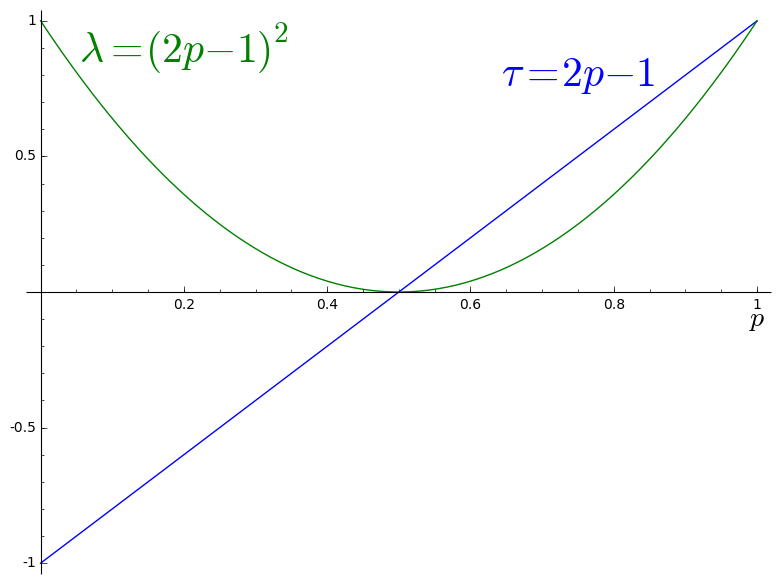
\includegraphics[scale=0.5]{figures/BC_Potenzial2.png}
\end{center}
\caption{The relation between the probability $p$, the
   I/O-correlation\index{I/O-correlation} $\tau$, and the
   potential\index{potential} $\lambda$}\label{fig-bool-pot}
\end{figure}

\begin{sagecode}
\begin{verbatim}

sage: plot1 = plot(2*x-1, (x,0,1))
sage: plot2 = plot((2*x - 1)**2, (x,0,1), color = 'green')
sage: xlabel = text('$p$', (1.0, -0.1), fontsize = 20, color = 'black')
sage: legend1 = text('$\tau = 2p - 1$', (0.75,0.8), fontsize = 30)
sage: legend2 = text('$\lambda = (2p - 1)^2$', (0.2,0.9), fontsize = 30,\\
        color = 'green')
sage: show(plot1 + plot2 + xlabel + legend1 + legend2)
\end{verbatim}
\caption{Plot of I/O-correlation\index{I/O-correlation} and
   potential\index{potential}}\label{Sage-code-bool-pot}
\end{sagecode}

Note that the key $k$ is the target of the attack. As long as it is
unknown, the value of $p_{F,\alpha,\beta,\kappa}(k)$ is also unknown.
Thus for cryptanalysis it makes sense to average the probabilities
of a linear relation over all keys:
\begin{equation}\label{eq-bool-avrg}
   p_{F,\alpha,\beta,\kappa} := \frac{1}{2^{n+l}}
      \#\{(a,k) \in \F_2^n \times \F_2^l \:|\:
           \kappa(k) = \alpha(a) + \beta(F(a,k)) \}.
\end{equation}
This average probability is determined, at least theoretically,
neglecting efficiency, by the definition of the cipher $F$ alone. Calculating
it however amounts to an exhaustion of all plaintexts and keys, and thus
is unrealistic for a realistic cipher with large block lengths.
We extend the definition for the ``average case'' also to
I/O-correlation\index{I/O-correlation} and potential\index{potential}\footnote{%
   Note that the I/O-correlation also is an average, but the potential is not!
}:
\[
   \tau_{F,\alpha,\beta,\kappa} := 2 p_{F,\alpha,\beta,\kappa} - 1,
\]
\[
   \lambda_{F,\alpha,\beta,\kappa} := \tau_{F,\alpha,\beta,\kappa}^2.
\]

Shamir\index{Shamir, Adi}\footnote{%
  Adi Shamir, Israeli cryptologist, co-inventor of the RSA cipher,
  $~^{\ast}$July 6, 1952
}
already in 1985 noticed that the S-boxes of DES\index{DES} admit
linear\index{linear relation}\index{relation!linear} relations with
conspicuous probabilities. However it took another seven years until
Matsui\index{Matsui, Mitsuru}\footnote{%
  Mitsuru Matsui, Japanese cryptologist, $~^{\ast}$September 16, 1961
}
(after first attempts by Gilbert and Chass� 1990 with the cipher FEAL)
succeeded in making systematic use of this observation. For
estimating\index{maximum likelihood estimation}\footnote{%
   This is a maximum likelihood estimation. One decides between
   several hypotheses (two in our case), and prefers the one
   hypothesis that attributes the highest probability to the observation.
}
$\kappa(k)$ he proceeded as follows (in the
case $p_{F,\alpha,\beta,\kappa} > \frac{1}{2}$, else complementary\footnote{%
  In the case $p_{F,\alpha,\beta,\kappa} = \frac{1}{2}$ the method is
  useless.
}):
\begin{enumerate}
   \item {\bf Collect} $N$ pairs of plaintexts and corresponding
      ciphertexts $(a_1,c_1), \ldots, (a_N,c_N)$.

   \item {\bf Count} the number
\[
    t := \# \{i = 1, \ldots, N \:|\: \alpha(a_i) + \beta(c_i) = 0\}.
\]

   \item {\bf Decide} by majority depending on $t$:
	  \begin{itemize}
	    \item If $t > \frac{N}{2}$, estimate $\kappa(k) = 0$.
	    \item If $t < \frac{N}{2}$, estimate $\kappa(k) = 1$.
	  \end{itemize}
\end{enumerate}
The case $t = \frac{N}{2}$ is worthless, however scarce---we might
randomize the decision between $0$ and $1$, or output a suitable
error code\footnote{%
   or both as in SageMath sample~\ref{Sage-code-bool-mats}
}. SageMath sample~\ref{Sage-code-bool-mats}
contains the program code. A concrete application follows as example
in the next subsection.

\begin{sagecode}
\begin{verbatim}

def Matsui_Test(a, b, pc, compl = False):
  """Matsui's test for linear cryptanalysis"""
  N = len(pc)
  results = []
  for pair in pc:
    ax = binScPr(a,pair[0])
    by = binScPr(b,pair[1])
    result = (ax + by) % 2
    results.append(result)
  t = 0
  for bb in results:
    if bb == 0:
      t = t + 1
  if 2*t > N:
    if compl:
      return [t,1,True]
    else:
      return [t,0,True]
  elif 2*t_0 < N:
    if compl:
      return [t,0,True]
    else:
      return [t,1,True]
  else:
    return [t,randint(0,1),False]
\end{verbatim}
\caption{Matsui's test\index{Matsui's test}\index{test!Matsui's}.
   The linear forms are {\tt a}
   for $\alpha$, and {\tt b} for $\beta$. The list {\tt pc} consists of
   {\tt N} pairs of plaintexts and corresponding ciphertexts. The Boolean
   value {\tt compl} indicates if the resulting bit must be inverted.
   The output is a triple consisting of the count {\tt t} of zeros,
   the guessed bit, and the Boolean value that indicates whether the
   bit is deterministic ({\tt True}) or (in the limit case) randomized
   ({\tt False}). We use the function {\tt binScPr} (``binary scalar
   product'') from SageMath sample~\ref{Sage-code-bool-div-bbl} in
   Appendix~\ref{ss-bool-conv}.}\label{Sage-code-bool-mats}
\end{sagecode}

If we detect a linear relation\index{linear relation}\index{relation!linear}
whose probability differs from $\frac{1}{2}$ in a sufficient way, then this
procedure will have a good success probability for sufficiently large $N$.
This allows to reduce the number of unknown key bits by 1, applying
elimination\index{elimination}.

As a theoretical result from these considerations we'll get a connection
between the number $N$ of needed plaintext blocks and the success
probability, see Table~\ref{tab-bool-N}.

The more linear relations with sufficiently high certainty the
attacker finds, the more she can reduce the size of the remaining
key space until finally an exhaustion\index{exhaustion} becomes
feasible. A concrete example in Section~\ref{ss-bool-mini} will
illustrate this.

\subsubsection*{Example}

For a concrete example with $n = l = 4$ we consider the Boolean
map\footnote{%
   By the way $f$ is the S-box\index{S-box} $\mathrm{S}_0$
   of {\sc Lucifer}\index{Lucifer}, a precursor of DES\index{DES}
   developed around 1970.
}
$f$ that is given by the values in Table~\ref{tab-bool-A1}, and
define the bitblock cipher
\[
    F\!: \F_2^4 \times \F_2^4 \longrightarrow \F_2^4 \quad
    \text{by } F(a,k) := f(a + k).
\]
SageMath sample~\ref{Sage-code-Luc-S0} defines this Boolean map
$f =$ {\tt S0}, using the classes {\tt BoolF} and {\tt BoolMap}
from Appendix~\ref{ss-bool-class}.
The columns of the defining matrix (implicit in the SageMath code)
just give the values of the map as they are also found
in the column $y = f(x)$ of Table~\ref{tab-bool-A1}.
(In other words, SageMath sample~\ref{Sage-code-Luc-S0} and
Table~\ref{tab-bool-A1} give equivalent definitions of the map $f$.)
A sample evaluation illustrates this (for the third column,
representing the argument {\tt 0010}).

\begin{sagecode}
\begin{verbatim}

f1 = BoolF([1,1,0,1,1,1,1,0,0,0,0,0,1,0,0,1])
f2 = BoolF([1,1,1,0,1,1,0,0,0,1,0,0,0,1,1,0])
f3 = BoolF([0,1,1,1,1,0,1,0,1,1,1,0,0,0,0,0])
f4 = BoolF([0,1,1,0,0,1,1,0,0,0,1,1,1,0,1,0])
S0 = BoolMap([f1,f2,f3,f4])
# Sample evaluation
sage: S0.valueAt([0,0,1,0])
[0, 1, 1, 1]
\end{verbatim}
\caption{A Boolean map (the S-box $\mathrm{S}_0$ of
   {\sc Lucifer})}\label{Sage-code-Luc-S0}
\end{sagecode}

We encrypt using the key $k = $ \verb:1000: (that we'll attack later as a
test case). For a linear relation we consider the linear forms
\[
     \alpha(a) = a_4, \quad \beta(c) = c_1 + c_2 + c_4, \quad \kappa(k) = k_4.
\]
In Section~\ref{ss-bool-bsp1} we'll see that with these linear forms
the relation $\kappa(k) = \alpha(a) + \beta(c)$ for $F$ has a quite
large probability. Table~\ref{tab-bool-mats} shows the ciphertexts
belonging to three plaintexts $a$ (that later we'll assume as known
plaintexts). The values of $c$ are taken from Table~\ref{tab-bool-A1}.
The number $t$ of observed values $0$ of $\alpha(a)$ + $\beta(c)$
is $t = 2$. Hence the majority decision gives the estimate $k_4 = 0$
(being in cheat mode we know it's correct).

\begin{table}
\begin{center}
\begin{tabular}{|c|c|c|c|} \hline
       $x$   & $y=f(x)$& $\alpha(x) = x_4$ & $\beta(y) = y_1+y_2+y_4$ \\ \hline
     0 0 0 0 & 1 1 0 0 &   0   &  0  \\
     0 0 0 1 & 1 1 1 1 &   1   &  1  \\
     0 0 1 0 & 0 1 1 1 &   0   &  0  \\
     0 0 1 1 & 1 0 1 0 &   1   &  1  \\
     0 1 0 0 & 1 1 1 0 &   0   &  0  \\
     0 1 0 1 & 1 1 0 1 &   1   &  1  \\
     0 1 1 0 & 1 0 1 1 &   0   &  0  \\
     0 1 1 1 & 0 0 0 0 &   1   &  0  \\
     1 0 0 0 & 0 0 1 0 &   0   &  0  \\
     1 0 0 1 & 0 1 1 0 &   1   &  1  \\
     1 0 1 0 & 0 0 1 1 &   0   &  1  \\
     1 0 1 1 & 0 0 0 1 &   1   &  1  \\
     1 1 0 0 & 1 0 0 1 &   0   &  0  \\
     1 1 0 1 & 0 1 0 0 &   1   &  1  \\
     1 1 1 0 & 0 1 0 1 &   0   &  0  \\
     1 1 1 1 & 1 0 0 0 &   1   &  1  \\ \hline
\end{tabular}
\end{center}
\caption{Value table of a Boolean map
  $f\!: \F_2^4 \longrightarrow \F_2^4$, and two linear forms}\label{tab-bool-A1}
\end{table}

\begin{table}
\begin{center}
\begin{tabular}{|c|c|c||ccc|}\hline
   $a$  & $a+k$ & $c$  & $\alpha(a)$ & $\beta(c)$ & $\alpha(a)$ + $\beta(c)$ \\
   \hline
   0010 & 1010  & 0011 &     0       &      1     &             1            \\
   0101 & 1101  & 0100 &     1       &      1     &             0            \\
   1010 & 0010  & 0111 &     0       &      0     &             0            \\
   \hline
\end{tabular}
\end{center}
\caption{Estimating a key bit after Matsui using three known
   plaintexts}\label{tab-bool-mats}
\end{table}

This was easily done with pencil and paper. However it might be instructive
to retrace the count in SageMath for a better understanding of more complex examples.
SageMath sample~\ref{Sage-code-Mats-Expl} provides this. It uses the function
{\tt xor}\index{XOR} from SageMath sample~\ref{Sage-code-bool-div-bbl} in Appendix~\ref{ss-bool-conv},
as well {\tt S0} from SageMath sample~\ref{Sage-code-Luc-S0}. The result
\mbox{\tt [2, 0, True]} says that we found $2$ zeroes among the counted values,
yielding the majority decision $0$, and the output parameter {\tt True} tells
that the decision was deterministic, not randomized.

\begin{sagecode}
\begin{verbatim}

sage: k = [1,0,0,0]
sage: alpha = [0,0,0,1]
sage: beta = [1,1,0,1]
sage: plist = [[0,0,1,0],[0,1,0,1],[1,0,1,0]]
sage: xlist = []
sage: xclist = []
sage: pclist = []
sage: for i in range(0,len(plist)):
....:     x = xor(plist[i],k)
....:     xlist.append(x)
....:     
sage: xlist
[[1, 0, 1, 0], [1, 1, 0, 1], [0, 0, 1, 0]]
sage: for i in range(0,len(plist)):
....:     val = S0.valueAt(xlist[i])
....:     xclist.append([xlist[i],val])
....:     pclist.append([plist[i],val])
....:     
sage: Matsui_Test(alpha,beta,pclist,False)
[2, 0, True]
\end{verbatim}
\caption{An example of Matsui's test\index{Matsui's test}}\label{Sage-code-Mats-Expl}
\end{sagecode}

\noindent How successful will this procedure be in general? We have to analyse the problems:
\begin{enumerate}
	\item How to find linear\index{linear relation}\index{relation!linear}
        relations of sufficiently high probabilities?
     \item Since in general bitblock\index{bitblock cipher} ciphers consist of
        several rounds\index{round} we ask:
	\begin{enumerate}
	  \item How to find useful linear relations for the round function of an
          iterated bitblock cipher?
	  \item How to combine these over the rounds as a linear relation for the
          complete cipher?
	  \item How to calculate the probability of a combined linear relation for
          the complete cipher from the probabilities for the single rounds?
	\end{enumerate}
\end{enumerate}

\noindent The answer to the first question and part (a) of the second one is: from the
linear\index{linear profile}\index{profile!linear} profile, see
Section~\ref{ss-bool-lpr}. The following partial questions lead to the
analysis of linear paths\index{linear path}\index{path!linear}, see
Section~\ref{ss-bool-path}, and the cumulation of probabilities, see
Theorem~\ref{thm-bool-rrnd}. For (c) finally we'll find a useful rule of thumb.

\subsection{Example A: A one-round cipher}\label{ss-bool-bsp1}

We consider examples that are much too simple for real
world applications but illustrate the principles of
linear\index{linear cryptanalysis}\index{cryptanalysis!linear}
cryptanalysis in an easily intelligible way. We always assume round
functions of the type $f(a+k)$, that is we add the key---or
an $n$-bit part of it---to the plaintext\footnote{%
   This is a quite special method of bringing the key into
   play but nevertheless realistic. The paradigmatic
   sample ciphers {\sc Lucifer}\index{Lucifer}, DES\index{DES},
   and AES\index{AES} do so. The term used with AES \cite{DaRi2002}
   is ``key-alternating cipher structure''.
} before applying a bijective
S-box $f\!: \F_2^n \longrightarrow \F_2^n$. The simplest model is
encryption by the formula
\[
   c = f(a+k),
\]
see\footnote{%
  The graphics here and later represent the map $f$ sometimes by the
  S-box S in the elementwise assignments.
} Figure~\ref{fig-bool-bsp0}.
This example is pointless because one block of known
plaintext\index{known plaintext}\index{plaintext!known} gives
a solution\footnote{%
   We assume that the attacker knows the inverse map $f^{-1}$ that
   is part of the decryption algorithm. One-way\index{one-way encryption}
   encryption methods that assume that $f^{-1}$ is not efficiently
   deducible from $f$ are the subject of another part of cryptography.
} for $k$:
\[
   k = f^{-1}(c) + a.
\]

\begin{figure}
\begin{center}
\begin{picture}(268,68)(0,0)
% Mengen
   \put(11,14){$\F_2^n$}
   \put(28,17){\vector(1,0){34}}
   \put(66,14){$\F_2^n$}
   \put(54,26){$\bigoplus$}
   \put(66,54){$\F_2^n$}
   \put(71,51){\vector(0,-1){28}}
   \put(83,17){\vector(1,0){34}}
   \put(94,20){$f$}
   \put(123,14){$\F_2^n$}

% Elemente
   \put(154,14){$a$}
   \put(165,17){\vector(1,0){28}}
   \put(165,14){\line(0,1){6}}
   \put(197,14){$b$}
   \put(197,54){$k$}
   \put(199,51){\vector(0,-1){28}}
   \put(197,51){\line(1,0){6}}
   \put(205,17){\vector(1,0){40}}
   \put(205,14){\line(0,1){6}}
   \put(214,14){\fcolorbox{black}{yellow}{S}}
   \put(251,14){$c$}

% Rahmen
   \put(0,0){\line(1,0){268}}
   \put(0,68){\line(1,0){268}}
   \put(0,0){\line(0,1){68}}
   \put(268,0){\line(0,1){68}}
\end{picture}
\end{center}
\caption{A (much too) simple example}\label{fig-bool-bsp0}
\end{figure}

\begin{figure}
\begin{center}
\begin{picture}(208,137)(0,0)
% Mengen
   \put(11,83){$\F_2^n$}
   \put(28,85){\vector(1,0){34}}
   \put(66,83){$\F_2^n$}
   \put(54,94){$\bigoplus$}
   \put(66,124){$\F_2^n$}
   \put(71,120){\vector(0,-1){28}}
   \put(83,85){\vector(1,0){34}}
   \put(94,88){$f$}
   \put(125,83){$\F_2^n$}
   \put(140,85){\vector(1,0){34}}
   \put(179,124){$\F_2^n$}
   \put(185,120){\vector(0,-1){28}}
   \put(168,94){$\bigoplus$}
   \put(179,83){$\F_2^n$}

% Elemente
   \put(23,14){$a$}
   \put(34,17){\vector(1,0){28}}
   \put(34,14){\line(0,1){6}}
   \put(71,14){$b$}
   \put(68,54){$k^{(0)}$}
   \put(74,51){\vector(0,-1){28}}
   \put(71,51){\line(1,0){6}}
   \put(80,17){\vector(1,0){40}}
   \put(80,14){\line(0,1){6}}
   \put(91,14){\fcolorbox{black}{yellow}{S}}
   \put(128,14){$b'$}
   \put(179,54){$k^{(1)}$}
   \put(185,51){\vector(0,-1){28}}
   \put(182,51){\line(1,0){6}}
   \put(142,17){\vector(1,0){28}}
   \put(142,14){\line(0,1){6}}
   \put(182,14){$c$}

% Rahmen
   \put(0,0){\line(1,0){208}}
   \put(0,137){\line(1,0){208}}
   \put(0,0){\line(0,1){137}}
   \put(208,0){\line(0,1){137}}
\end{picture}
\end{center}
\caption{Example A: A One-Round Cipher}\label{fig-bool-bspA}
\end{figure}

\begin{figure}
\begin{center}
\begin{picture}(85,68)(0,0)
   \put(6,48){$\F_2^n$}
   \put(23,51){\vector(1,0){40}}
   \put(40,54){$f$}
   \put(68,48){$\F_2^n$}
   \put(40,9){$\F_2$}
   \put(17,43){\vector(1,-1){23}}
   \put(17,26){$\alpha$}
   \put(68,43){\vector(-1,-1){23}}
   \put(60,26){$\beta$}
   \put(38,31){$\stackrel{p}{\approx}$}

% Rahmen
   \put(0,0){\line(1,0){85}}
   \put(0,68){\line(1,0){85}}
   \put(0,0){\line(0,1){68}}
   \put(85,0){\line(0,1){68}}
\end{picture}
\end{center}
\caption{Diagram for an ``approximative'' linear
   relation\index{linear relation}\index{relation!linear}}\label{fig-bool-appr}
\end{figure}

The somewhat more involved example A stops this attack:
\[
   c = f(a+k^{(0)}) + k^{(1)}
\]
(see Figure~\ref{fig-bool-bspA}). This is the simplest example for which
the method of
linear cryptanalysis\index{linear cryptanalysis}\index{cryptanalysis!linear}
makes sense: Let $(\alpha,\beta)$ be a pair of linear\index{linear form}
forms with
\begin{equation}\label{eq-bool-prob}
     \beta\circ f(x) \stackrel{p}{\approx} \alpha(x),
\end{equation}
where the symbol $\stackrel{p}{\approx}$ reads as ``equal with
probability $p$'', or in other words
\[
     p = p_{f,\alpha,\beta} :=
     \frac{1}{2^{n}} \cdot \#\{x \in \F_2^n \:|\: \beta\circ f(x) = \alpha(x) \}.
\]
The diagram in Figure~\ref{fig-bool-appr} illustrates Formula~(\ref{eq-bool-prob}).
Note that the linear form $\kappa$ of the general theory is implicit
in the present context: Since the key bits are simply added to plaintext
and (``intermediary'') ciphertext we have $\kappa = \alpha$ for $k^{(0)}$,
and $\kappa = \beta$ for $k^{(1)}$, hence
$\kappa(k^{(0)}, k^{(1)}) = \alpha(k^{(0)}) + \beta(k^{(1)})$.

How does this scenario fit the general situation from Section~\ref{ss-bool-lka}?
In example~A we have
\begin{itemize}
   \item key length $l = 2n$, key space $\F_2^{2n}$, and
      keys of the form $k = (k^{(0)},k^{(1)})$ with $k^{(0)}, k^{(1)} \in \F_2^n$.
   \item The cipher is defined by the map
\[
     F\!: \F_2^n \times \F_2^n \times \F_2^n \longrightarrow \F_2^n,
     \quad (a, k^{(0)}, k^{(1)}) \mapsto f(a + k^{(0)}) + k^{(1)}.
\]
   \item The linear form $\kappa\!: \F_2^n \times \F_2^n \longrightarrow \F_2$
      is $\kappa(k^{(0)},k^{(1)}) = \alpha(k^{(0)}) + \beta(k^{(1)})$.
\end{itemize}
Hence the probability of a linear relation for a fixed key
\mbox{$k = (k^{(0)},k^{(1)})$} is
\begin{eqnarray*}
    p_{F,\alpha,\beta,\kappa}(k) & = & \frac{1}{2^n} \cdot
      \#\{a \in \F_2^n \:|\: \kappa(k) = \alpha(a) + \beta(F(a,k)) \} \\
     & = & \frac{1}{2^n} \cdot
      \#\{a \in \F_2^n \:|\: \alpha(k^{(0)}) + \beta(k^{(1)}) = \alpha(a) + \beta(f(a + k^{(0)}) + k^{(1)}) \} \\
     & = & \frac{1}{2^n} \cdot
      \#\{a \in \F_2^n \:|\: \alpha(k^{(0)}) = \alpha(a) + \beta(f(a + k^{(0)})) \},
\end{eqnarray*}
where we omitted $\beta(k^{(1)})$ that occurs on both sides of the equation
inside the curly set brackets.

This expression is independent of $k^{(1)}$, and the slightly rewritten
equation
\[
     p_{F,\alpha,\beta,\kappa}(k) = \frac{1}{2^n} \cdot
      \#\{a \in \F_2^n \:|\: \alpha(a + k^{(0)}) = \beta(f(a + k^{(0)})) \}
\]
shows that it assumes the same value for all $k^{(0)}$: With $a$ also
$a + k^{(0)}$ runs through all of $\F_2^n$ for a fixed $k^{(0)}$.
Therefore this value must agree with the mean value over all $k$:
\[
     p_{F,\alpha,\beta,\kappa}(k) = p_{F,\alpha,\beta,\kappa} = \frac{1}{2^n} \cdot
      \#\{x \in \F_2^n \:|\: \alpha(x) = \beta(f(x)) \} = p.
\]
This consideration shows:

\begin{theorem}
    In the scenario of example~A the probability $p_{F,\alpha,\beta,\kappa}(k)$
    assumes the same value
\[
     p = \frac{1}{2^n} \cdot \#\{x \in \F_2^n \:|\: \alpha(x) = \beta(f(x)) \}
\]
   for all keys $k \in \F_2^{2n}$. In particular $p$ coincides with the mean value
   from Equation~{\rm (\ref{eq-bool-avrg})}.
\end{theorem}

Using the notations from Figure~\ref{fig-bool-bspA} we have
\begin{align*}
   \beta(c) & = \beta(b' + k^{(1)}) = \beta(b') + \beta(k^{(1)}) \\
            & \stackrel{p}{\approx} \alpha(b) + \beta(k^{(1)})
                   = \alpha(a + k^{(0)}) + \beta(k^{(1)})
                        = \alpha(a) + \alpha(k^{(0)}) + \beta(k^{(1)}).
\end{align*}
This yields a linear\index{linear relation}\index{relation!linear}
relation for the bits of the key $k = (k_1,k_2)$:
\[
   \alpha(k^{(0)}) + \beta(k^{(1)}) \stackrel{p}{\approx} \alpha(a) + \beta(c).
\]
Treating the complementary relation
\[
   \beta\circ f(x) \stackrel{1-p}{\approx} \alpha(x) + 1
\]
in an analoguous way we get:

\begin{theorem}
   In the scenario of example A let $(\alpha,\beta)$ be a pair of
   linear\index{linear form} forms for $f$ with probability $p$ as in
   Formula~{\rm (\ref{eq-bool-prob})}.
   Then $\hat{p} = \max\{p, 1-p\}$ is the success probability
   for determing a single key bit by this linear
   relation\index{linear relation}\index{relation!linear} given
   {\em one} known\index{known plaintext}\index{plaintext!known}
   plaintext block.
\end{theorem}

\subsubsection*{Example}

Take $n = 4$, and for $f$ take the S-box
$\mathrm{S}_0$ of {\sc Lucifer}\index{Lucifer}. As the two rightmost
columns of Table~\ref{tab-bool-A1} show the linear relation defined
by $(\alpha,\beta)$, where $\alpha(x) = x_4$ and $\beta(y) = y_1+y_2+y_4$,
has probability\footnote{%
   providing strong evidence that the designers of {\sc Lucifer}\index{Lucifer}
   weren't aware of linear\index{linear cryptanalysis}\index{cryptanalysis!linear}
   cryptanalysis
} $p_{f,\alpha,\beta} = \frac{14}{16} = \frac{7}{8}$.

As concrete round\index{round key} keys take $k_0 = $\verb:1000: and $k_1 = $\verb:0001:.
Table~\ref{tab-bool-linrel}, running through all possible $16$ plaintexts,
shows that $\alpha(a)+\beta(c)$ assumes the value $1 =\alpha(k_0) + \beta(k_1)$
for this partial sum of key bits exactly $14$ times---as expected.

\begin{table}
\begin{center}
\begin{tabular}{|cccc|c|} \hline
  $a$  & $b$  & $b'$ & $c$  & $\alpha(a)+\beta(c)$ \\ \hline
  0000 & 1000 & 0010 & 0011 & 1 \\
  0001 & 1001 & 0110 & 0111 & 1 \\
  0010 & 1010 & 0011 & 0010 & 0 \\
  0011 & 1011 & 0001 & 0000 & 1 \\
  0100 & 1100 & 1001 & 1000 & 1 \\
  0101 & 1101 & 0100 & 0101 & 1 \\
  0110 & 1110 & 0101 & 0100 & 1 \\
  0111 & 1111 & 1000 & 1001 & 1 \\
  1000 & 0000 & 1100 & 1101 & 1 \\
  1001 & 0001 & 1111 & 1110 & 1 \\
  1010 & 0010 & 0111 & 0110 & 1 \\
  1011 & 0011 & 1010 & 1011 & 1 \\
  1100 & 0100 & 1110 & 1111 & 1 \\
  1101 & 0101 & 1101 & 1100 & 1 \\
  1110 & 0110 & 1011 & 1010 & 1 \\
  1111 & 0111 & 0000 & 0001 & 0 \\
  \hline
\end{tabular}
\end{center}
\caption{A linear relation for the key bits ($b$ arises from $a$ by adding
   $k^{(0)}$, resulting in ``flipping'' the first bit, $b'$ from $b$ by applying
   $f$, and $c$ from $b'$ by adding $k^{(1)}$.}\label{tab-bool-linrel}
\end{table}

How large is the success probability $p_N$ of correctly estimating
this partial sum, assuming $N = 1, 2, \ldots$ random
known\index{known plaintext}\index{plaintext!known} plaintexts
from the set of $2^n$ possible plaintexts? (For given linear forms
$\alpha$ and $\beta$ with $p = p_{f,\alpha,\beta}$.) This is
exactly the scenario of the hypergeometric
distribution\index{hypergeometric distribution}\index{distribution!hypergeometric}\footnote{%
   that we won't explain here
}.
Therefore we have:

\begin{theorem}
  In example A let $(\alpha,\beta)$ be a pair of linear forms that
  defines a linear relation for $f$ with probability $p$.
  Then the success probability for determining a key bit by this linear
  relation\index{linear relation}\index{relation!linear} from $N$ known
  plaintexts is the cumulated probability $p_N = p_N^{(s)}$ of the
  hypergeometric distribution with parameters $2^n$,
  $s = \hat{p}\cdot 2^n$, and $N$ where $\hat{p} = \max\{p, 1-p\}$.
\end{theorem}

If we neglect exact mathematical reasoning and work with asymptotic
approximations (as is common in applied statistics), then we can
replace the hypergeometric
distribution\index{hypergeometric distribution}\index{distribution!hypergeometric}
by the normal distribution\index{normal distribution}\index{distribution!normal}.
The usual (quite vaguely stated) conditions for this approximation are ``$p$ not too
different from $\frac{1}{2}$, $N \ll 2^n$, but $N$ not too small.''
This gives the formula
\begin{equation}\label{equ-bool-N}
  p_N \approx \frac{1}{\sqrt{2\pi}} \cdot
                      \int_{-\infty}^{\sqrt{N\lambda}} e^{-t^2/2}\,dt,
\end{equation}
where $\lambda = (2p - 1)^2$ is the potential\index{potential} of the
linear relation. The values associated with the normal distribution\footnote{%
   Instead of the approximation by the normal distribution we could
   directly use the hypergeometric
   distribution\index{hypergeometric distribution}\index{distribution!hypergeometric}.
   This would, in particular for small $N$, give a more precise value
   but not a closed formula as simple as (\ref{equ-bool-N}).
} are well-known
and yield Table~\ref{tab-bool-N}. To get a success probability of
about $95\%$ we need $N \approx \frac{3}{\lambda}$ known
plaintexts\index{known plaintext}\index{plaintext!known}
according to the table. In the concrete example above
we had $p = \frac{7}{8}$, hence $\lambda = \frac{9}{16}$,
and the number of known plaintexts needed for a $95\%$
success probability is $N \approx 5$. Using Table~\ref{tab-bool-mats}
we succeeded with only $N = 3$ plaintexts. This is no great surprise
because the a-priori probability of this success is about 90\% (for
$N\lambda = \frac{27}{16} \approx 1,68\ldots$)\footnote{%
   Here the condition ``$N$ not too small'' for the approximation by the
   normal distribution\index{normal distribution}\index{distribution!normal}
   is more than arguable. However determining the exact values for the hypergeometric
   distribution\index{hypergeometric distribution}\index{distribution!hypergeometric}
   is easy:
   Consider an urn containing $16$ balls, $14$ black ones and
   $2$ white ones, and draw $3$ balls by random. Then the probability of all
   of them being black is $\frac{26}{40}$, the probability of two being black
   and one being white is $\frac{13}{40}$. Hence the probability of at least
   two balls being black is $\frac{39}{40} = 97,5\%$. This is clearly more
   than the 90\% from the approximation~(\ref{equ-bool-N}).
   The remaining probabilities are $\frac{1}{40}$ for exactly one black
   ball, and $0$ for three white balls.
}.

\begin{table}
\begin{center}
  \begin{tabular}{|c|ccccccc|} \hline
		$N\lambda$ & $1$ & $2$ & $3$ & $4$ & \ldots & $8$ & $9$ \\
		$p_N$ & $84,1\%$ & $92,1\%$ & $95,8\%$ & $97,7\%$ & \ldots &
		                      $99,8\%$ & $99,9\%$ \\ \hline
  \end{tabular}
\end{center}
\caption{Dependence of the success probability on the number of known
   plaintexts\index{known plaintext}\index{plaintext!known}}\label{tab-bool-N}
\end{table}

\subsection{Approximation Table\index{approximation table},
   Correlation Matrix\index{correlation matrix}, and Linear
   Profile\index{linear profile}\index{profile!linear}}\label{ss-bool-lpr}

Linear relations\index{linear relation}\index{relation!linear} for a Boolean
map\index{Boolean map}\index{map!Boolean} (or S-box\index{S-box})
$f\!\!: \F_2^n \longrightarrow \F_2^q$ are true with certain frequencies
(or probabilities). We collect these frequencies in a matrix of size
$2^n \times 2^q$, called the
{\bf approximation table\index{approximation table}}\footnote{%
   When using references be aware that often all entries are diminished
   by $2^{n-1}$, for example by the SageMath function
   {\tt linear\_approximation\_matrix()}.
}\label{fn-lin-appr}
of $f$. This table gives, for each pair $(\alpha,\beta)$ of linear
forms\index{linear form}, the number of arguments $x$ where
\mbox{$\beta\circ f(x) = \alpha(x)$.}
Table~\ref{tab-bool-s0} shows the approximation table of the S-box $\mathrm{S}_0$
of {\sc Lucifer}\index{Lucifer}. The entry $16$ in the upper left corner
says that the relation $0 = 0$ is true in all $16$
possible cases. At the same time $16$ is the common denominator by which
we have to divide all other entries to get the probabilities. In the general case
the upper left corner would be  $2^n$. The remaining entries of the first column
(corresponding to $\beta = 0$) are $8$ because each non-zero
linear form\index{linear form} $\alpha$ takes the value $0$ in exactly half
of all cases, that is $8$ times\footnote{%
   In the language of linear algebra\index{linear algebra}\index{algebra!linear}
   we express this fact as:
   The kernel of a linear form\index{linear form} $\neq 0$ is a subspace of
   dimension $n-1$.
}. For the first row an analogous argument is true---provided that $f$ is
bijective\footnote{%
   In the general case where $q$ could be $\neq n$ we would use the concept
   ``balanced\index{balanced}'' that means that all preimages have the same
   size. Of course a map can be balanced only in the case $q \leq n$.
}.

\begin{table}
\begin{center}
\begin{tabular}{|c|cccccccccccccccc|} \hline
     & 0 & 1 & 2 & 3 & 4 & 5 & 6 & 7 & 8 & 9 &10 &11 &12 &13 &14 &15 \\ \hline
   0 &16 & 8 & 8 & 8 & 8 & 8 & 8 & 8 & 8 & 8 & 8 & 8 & 8 & 8 & 8 & 8 \\
   1 & 8 & 6 & 6 & 8 & 8 & 6 & 6 & 8 & 8 & 6 & 6 & 8 & 8 &14 & 6 & 8 \\
   2 & 8 &10 & 8 & 6 & 4 & 6 & 8 & 6 & 6 &12 & 6 & 8 &10 & 8 & 6 & 8 \\
   3 & 8 &12 &10 & 6 &12 & 8 &10 & 6 & 6 & 6 & 8 & 8 &10 &10 & 8 & 8 \\
   4 & 8 & 8 & 4 & 8 & 8 & 8 & 8 & 4 &10 & 6 & 6 & 6 &10 & 6 &10 &10 \\
   5 & 8 &10 &10 &12 & 8 &10 & 6 & 8 &10 & 8 & 4 &10 &10 & 8 & 8 & 6 \\
   6 & 8 &10 & 8 &10 & 8 &10 & 8 &10 & 8 &10 & 8 & 2 & 8 &10 & 8 &10 \\
   7 & 8 & 8 &10 & 6 & 8 & 8 & 2 & 6 & 8 & 8 &10 & 6 & 8 & 8 &10 & 6 \\
   8 & 8 & 8 & 6 &10 & 6 &10 & 8 & 8 & 4 & 8 &10 &10 &10 &10 &12 & 8 \\
   9 & 8 &10 & 8 &10 & 6 & 4 &10 & 8 & 8 & 6 & 8 & 6 & 6 & 8 &10 & 4 \\
  10 & 8 & 6 &10 & 8 & 6 & 8 & 8 &10 & 6 & 4 & 8 & 6 &12 & 6 & 6 & 8 \\
  11 & 8 &12 & 8 & 8 & 6 & 6 & 6 &10 &10 & 6 &10 &10 & 8 & 8 & 8 &12 \\
  12 & 8 & 8 &10 &10 & 6 &10 & 8 & 4 & 6 & 6 & 8 & 8 & 4 & 8 & 6 &10 \\
  13 & 8 & 6 &12 & 6 & 6 & 8 &10 & 8 &10 & 8 & 6 & 8 & 8 &10 &12 & 8 \\
  14 & 8 & 6 &10 &12 &10 & 4 & 8 & 6 & 8 &10 &10 & 8 &10 & 8 & 8 &10 \\
  15 & 8 & 8 & 8 & 8 &10 & 6 & 6 &10 & 4 & 8 & 4 & 8 & 6 & 6 &10 &10 \\ \hline
\end{tabular}
\end{center}
\caption{Approximation table of the S-box $\mathrm{S}_0$ of {\sc Lucifer}\index{Lucifer}.
   Row and column indices are linear forms represented by integers,
   see Section~\ref{ss-bool-repr}.
   To get the probabilities divide by 16.}\label{tab-bool-s0}
\end{table}

\begin{table}
\begin{center}
\begin{tabular}{|c|cccccccccccccccc|} \hline
     & 0 & 1 & 2 & 3 & 4 & 5 & 6 & 7 & 8 & 9 &10 &11 &12 &13 &14 &15 \\ \hline
   0 & 1 & 0 & 0 & 0 & 0 & 0 & 0 & 0 & 0 & 0 & 0 & 0 & 0 & 0 & 0 & 0 \\
   1 & 0 &$-\frac{1}{4}$&$-\frac{1}{4}$& 0 & 0 &$-\frac{1}{4}$&$-\frac{1}{4}$& 0 & 0 &$-\frac{1}{4}$&$-\frac{1}{4}$& 0 & 0 &$\frac{3}{4}$&$-\frac{1}{4}$& 0 \\
   2 & 0 &$\frac{1}{4}$& 0 & $-\frac{1}{4}$ &$-\frac{1}{2}$& $-\frac{1}{4}$ & 0 & $-\frac{1}{4}$ & $-\frac{1}{4}$ &$\frac{1}{2}$& $-\frac{1}{4}$ & 0 &$\frac{1}{4}$& 0 & $-\frac{1}{4}$ & 0 \\
   3 & 0 &$\frac{1}{2}$&$\frac{1}{4}$& $-\frac{1}{4}$ &$\frac{1}{2}$& 0 &$\frac{1}{4}$& $-\frac{1}{4}$ & $-\frac{1}{4}$ & $-\frac{1}{4}$ & 0 & 0 &$\frac{1}{4}$&$\frac{1}{4}$& 0 & 0 \\
   4 & 0 & 0 &$-\frac{1}{2}$& 0 & 0 & 0 & 0 &$-\frac{1}{2}$&$\frac{1}{4}$& $-\frac{1}{4}$ & $-\frac{1}{4}$ & $-\frac{1}{4}$ &$\frac{1}{4}$& $-\frac{1}{4}$ &$\frac{1}{4}$&$\frac{1}{4}$\\
   5 & 0 &$\frac{1}{4}$&$\frac{1}{4}$&$\frac{1}{2}$& 0 &$\frac{1}{4}$& $-\frac{1}{4}$ & 0 &$\frac{1}{4}$& 0 &$-\frac{1}{2}$&$\frac{1}{4}$&$\frac{1}{4}$& 0 & 0 & $-\frac{1}{4}$ \\
   6 & 0 &$\frac{1}{4}$& 0 &$\frac{1}{4}$& 0 &$\frac{1}{4}$& 0 &$\frac{1}{4}$& 0 &$\frac{1}{4}$& 0 &$-\frac{3}{4}$& 0 &$\frac{1}{4}$& 0 &$\frac{1}{4}$\\
   7 & 0 & 0 &$\frac{1}{4}$& $-\frac{1}{4}$ & 0 & 0 &$-\frac{3}{4}$& $-\frac{1}{4}$ & 0 & 0 &$\frac{1}{4}$& $-\frac{1}{4}$ & 0 & 0 &$\frac{1}{4}$& $-\frac{1}{4}$ \\
   8 & 0 & 0 & $-\frac{1}{4}$ &$\frac{1}{4}$& $-\frac{1}{4}$ &$\frac{1}{4}$& 0 & 0 &$-\frac{1}{2}$& 0 &$\frac{1}{4}$&$\frac{1}{4}$&$\frac{1}{4}$&$\frac{1}{4}$&$\frac{1}{2}$& 0 \\
   9 & 0 &$\frac{1}{4}$& 0 &$\frac{1}{4}$& $-\frac{1}{4}$ &$-\frac{1}{2}$&$\frac{1}{4}$& 0 & 0 & $-\frac{1}{4}$ & 0 & $-\frac{1}{4}$ & $-\frac{1}{4}$ & 0 &$\frac{1}{4}$&$-\frac{1}{2}$\\
  10 & 0 & $-\frac{1}{4}$ &$\frac{1}{4}$& 0 & $-\frac{1}{4}$ & 0 & 0 &$\frac{1}{4}$& $-\frac{1}{4}$ &$-\frac{1}{2}$& 0 & $-\frac{1}{4}$ &$\frac{1}{2}$& $-\frac{1}{4}$ & $-\frac{1}{4}$ & 0 \\
  11 & 0 &$\frac{1}{2}$& 0 & 0 & $-\frac{1}{4}$ & $-\frac{1}{4}$ & $-\frac{1}{4}$ &$\frac{1}{4}$&$\frac{1}{4}$& $-\frac{1}{4}$ &$\frac{1}{4}$&$\frac{1}{4}$& 0 & 0 & 0 &$\frac{1}{2}$\\
  12 & 0 & 0 &$\frac{1}{4}$&$\frac{1}{4}$& $-\frac{1}{4}$ &$\frac{1}{4}$& 0 &$-\frac{1}{2}$& $-\frac{1}{4}$ & $-\frac{1}{4}$ & 0 & 0 &$-\frac{1}{2}$& 0 & $-\frac{1}{4}$ &$\frac{1}{4}$\\
  13 & 0 & $-\frac{1}{4}$ &$\frac{1}{2}$& $-\frac{1}{4}$ & $-\frac{1}{4}$ & 0 &$\frac{1}{4}$& 0 &$\frac{1}{4}$& 0 & $-\frac{1}{4}$ & 0 & 0 &$\frac{1}{4}$&$\frac{1}{2}$& 0 \\
  14 & 0 & $-\frac{1}{4}$ &$\frac{1}{4}$&$\frac{1}{2}$&$\frac{1}{4}$&$-\frac{1}{2}$& 0 & $-\frac{1}{4}$ & 0 &$\frac{1}{4}$&$\frac{1}{4}$& 0 &$\frac{1}{4}$& 0 & 0 &$\frac{1}{4}$\\
  15 & 0 & 0 & 0 & 0 &$\frac{1}{4}$& $-\frac{1}{4}$ & $-\frac{1}{4}$ &$\frac{1}{4}$&$-\frac{1}{2}$& 0 &$-\frac{1}{2}$& 0 & $-\frac{1}{4}$ & $-\frac{1}{4}$ &$\frac{1}{4}$&$\frac{1}{4}$\\ \hline
\end{tabular}
\end{center}\caption{Correlation matrix of the S-box $\mathrm{S}_0$ of {\sc Lucifer}\index{Lucifer}.
   Row and column indices are linear forms represented by integers.}\label{tab-bool-corr}
\end{table}

\begin{table}
\begin{center}
\begin{tabular}{|c|cccccccccccccccc|} \hline
  &0& 1            & 2            & 3            & 4            & 5            & 6            & 7            
     & 8            & 9            &10            &11            &12            &13            &14            &15            \\
\hline
 0&1& 0            & 0            & 0            & 0            & 0            & 0            & 0            
     & 0            & 0            & 0            & 0            & 0            & 0            & 0            & 0            \\
 1&0&$\frac{1}{16}$&$\frac{1}{16}$& 0            & 0            &$\frac{1}{16}$&$\frac{1}{16}$& 0            
     & 0            &$\frac{1}{16}$&$\frac{1}{16}$& 0            & 0            &$\frac{9}{16}$&$\frac{1}{16}$& 0            \\
 2&0&$\frac{1}{16}$& 0            &$\frac{1}{16}$&$\frac{1}{4}$ &$\frac{1}{16}$& 0            &$\frac{1}{16}$&$\frac{1}{16}$
     &$\frac{1}{4}$ &$\frac{1}{16}$& 0            &$\frac{1}{16}$& 0            &$\frac{1}{16}$& 0            \\
 3&0&$\frac{1}{4}$ &$\frac{1}{16}$&$\frac{1}{16}$&$\frac{1}{4}$ & 0            &$\frac{1}{16}$&$\frac{1}{16}$&$\frac{1}{16}$
     &$\frac{1}{16}$& 0            & 0            &$\frac{1}{16}$&$\frac{1}{16}$& 0            & 0            \\
 4&0& 0            &$\frac{1}{4}$ & 0            & 0            & 0            & 0            &$\frac{1}{4}$ &$\frac{1}{16}$
     &$\frac{1}{16}$&$\frac{1}{16}$&$\frac{1}{16}$&$\frac{1}{16}$&$\frac{1}{16}$&$\frac{1}{16}$&$\frac{1}{16}$\\
 5&0&$\frac{1}{16}$&$\frac{1}{16}$&$\frac{1}{4}$ & 0            &$\frac{1}{16}$&$\frac{1}{16}$& 0            &$\frac{1}{16}$
     & 0            &$\frac{1}{4}$ &$\frac{1}{16}$&$\frac{1}{16}$& 0            & 0            &$\frac{1}{16}$\\
 6&0&$\frac{1}{16}$& 0            &$\frac{1}{16}$& 0            &$\frac{1}{16}$& 0            &$\frac{1}{16}$& 0            
     &$\frac{1}{16}$& 0            &$\frac{9}{16}$& 0            &$\frac{1}{16}$& 0            &$\frac{1}{16}$\\
 7&0& 0            &$\frac{1}{16}$&$\frac{1}{16}$& 0            & 0            &$\frac{9}{16}$&$\frac{1}{16}$& 0            
     & 0            &$\frac{1}{16}$&$\frac{1}{16}$& 0            & 0            &$\frac{1}{16}$&$\frac{1}{16}$\\
 8&0& 0            &$\frac{1}{16}$&$\frac{1}{16}$&$\frac{1}{16}$&$\frac{1}{16}$& 0            & 0            &$\frac{1}{4}$ 
     & 0            &$\frac{1}{16}$&$\frac{1}{16}$&$\frac{1}{16}$&$\frac{1}{16}$&$\frac{1}{4}$ & 0            \\
 9&0&$\frac{1}{16}$& 0            &$\frac{1}{16}$&$\frac{1}{16}$&$\frac{1}{4}$&$\frac{1}{16}$& 0            & 0            
     &$\frac{1}{16}$& 0            &$\frac{1}{16}$&$\frac{1}{16}$& 0            &$\frac{1}{16}$&$\frac{1}{4}$ \\
10&0&$\frac{1}{16}$&$\frac{1}{16}$& 0            &$\frac{1}{16}$& 0            & 0            &$\frac{1}{16}$&$\frac{1}{16}$
     &$\frac{1}{4}$ & 0            &$\frac{1}{16}$&$\frac{1}{4}$ &$\frac{1}{16}$&$\frac{1}{16}$& 0            \\
11&0&$\frac{1}{4}$ & 0            & 0            &$\frac{1}{16}$&$\frac{1}{16}$&$\frac{1}{16}$&$\frac{1}{16}$&$\frac{1}{16}$
     &$\frac{1}{16}$&$\frac{1}{16}$&$\frac{1}{16}$& 0            & 0            & 0            &$\frac{1}{4}$ \\
12&0& 0            &$\frac{1}{16}$&$\frac{1}{16}$&$\frac{1}{16}$&$\frac{1}{16}$& 0            &$\frac{1}{4}$ &$\frac{1}{16}$
     &$\frac{1}{16}$& 0            & 0            &$\frac{1}{4}$ & 0            &$\frac{1}{16}$&$\frac{1}{16}$\\
13&0&$\frac{1}{16}$&$\frac{1}{4}$&$\frac{1}{16}$&$\frac{1}{16}$& 0            &$\frac{1}{16}$& 0            &$\frac{1}{16}$
     & 0            &$\frac{1}{16}$& 0            & 0            &$\frac{1}{16}$&$\frac{1}{4}$ & 0 \\
14&0&$\frac{1}{16}$&$\frac{1}{16}$&$\frac{1}{4}$ &$\frac{1}{16}$&$\frac{1}{4}$ & 0            &$\frac{1}{16}$& 0            
     &$\frac{1}{16}$&$\frac{1}{16}$& 0            &$\frac{1}{16}$& 0            & 0            &$\frac{1}{16}$\\
15&0& 0            & 0            & 0            &$\frac{1}{16}$&$\frac{1}{16}$&$\frac{1}{16}$&$\frac{1}{16}$&$\frac{1}{4}$ 
     & 0            &$\frac{1}{4}$ & 0            &$\frac{1}{16}$&$\frac{1}{16}$&$\frac{1}{16}$&$\frac{1}{16}$\\
\hline
\end{tabular}
\end{center}\caption{Linear profile of the S-box $\mathrm{S}_0$ of {\sc Lucifer}\index{Lucifer}.
   Row and column indices are linear forms represented by integers.}\label{tab-bool-lp0}
\end{table}

The {\bf correlation matrix}\index{correlation matrix} and the
{\bf linear profile}\index{linear profile}\index{profile!linear}\footnote{%
   also called linearity profile\index{linearity profile}. Not to be
   confused with the linear complexity
   profile\index{linear complexity profile}\index{complexity profile!linear}
   of a bit sequence that is defined by linear feedback shift registers
   (LFSRs)\index{LFSR} and sometimes also called linearity profile.
   }
are the analogous matrices whose entries are the
I/O-correlations\index{I/O-correlation} or the potentials\index{potential}
of the corresponding linear relations. The
correlation matrix\index{correlation matrix} arises from the
approximation table\index{approximation table} by first dividing the
entries by $2^n$ (getting the probabilities $p$) and then transforming
the probabilities to I/O-correlations\index{I/O-correlation} by the
formula $\tau = 2p - 1$. To get the linear
profile\index{linear profile}\index{profile!linear} we have to
square the single entries of the correlation matrix\index{correlation matrix}.

For $\mathrm{S}_0$ Table~\ref{tab-bool-corr} shows the correlation
matrix\index{correlation matrix}, and Table~\ref{tab-bool-lp0}, the
linear profile\index{linear profile}\index{profile!linear}.
Here again the first rows and columns hit the eye: The zeroes tell
that a linear relation\index{linear relation}\index{relation!linear}
involving the linear form $0$ has potential $0$, hence is useless.
The $1$ in the upper left corner says that the relation $0 = 0$ holds
for any arguments, but is useless too. In the previous subsection we picked the
pair $(\alpha,\beta)$ where $\alpha(x) = x_4$ (represented by \verb:0001:
$\hat{=}\, 1$) and $\beta(y) = y_1+y_2+y_4$ (represented \verb:1101:
$\hat{=}\, 13$) in row 1, column 13. It assumes the maximum value\footnote{%
  We ignore the true, but useless, maximum value $1$ in the upper left corner.
} $\frac{9}{16}$ for the potential that moreover also occurs
at the coordinates $(6,11)$ and $(7,6)$.

\subsubsection*{Efficient Calculation by Fourier Transformation}

We can get the approximation table in the ``naive'' way by counting,
and then derive the correlation matrix and the linear profile by
a simple (elementwise) transformation. A more efficient algorithm
uses the Fourier\footnote{%
   Joseph Fourier\index{Fourier, Joseph}, French mathematician and physicist,
   March 21, 1768 -- May 16, 1830
} transformation\index{Fourier transformation}. In the binary case it is
especially simple, and due to historically independent inventions
is also called Hadamard\footnote{%
   Jacques Hadamard\index{Hadamard, Jacques}, French mathematician,
   December 8, 1865 -- October 17, 1963
} transformation\index{Hadamard transformation}, or Walsh\footnote{%
   Joseph L. Walsh\index{Walsh, Joseph L.}, American mathematician,
   September 21, 1895 -- December 6, 1973
} transformation\index{Walsh transformation}.
It transforms a {\em real valued} (!) function
$\varphi\!: \F_2^m \longrightarrow \R$ into another real valued
function $\hat{\varphi}\!: \F_2^m \longrightarrow \R$ defined by\footnote{%
   This is a special case of the discrete Fourier
   transformation\index{Fourier transformation!discrete}. In the
   general case we would use the complex $N$-th root of
   unity\index{root of unity} $\zeta = e^{2\pi i/N}$ instead of $-1$,
   and transform complex valued functions over the ring $\Z/N\Z$, instead
   over $\F_2 = \Z/2\Z$---or functions on $\Z^m$ that have period $N$ in
   each of the variables.
   In the binary case $N = 2$, and the 2nd root of unity $-1$ is
   real, so we only need to consider real valued functions.
}
\[
  \hat{\varphi}(u) := \sum_{x \in \F_2^m} \varphi(x)\cdot (-1)^{u\cdot x}.
\]
Here $u\cdot x$ is the canonical scalar product\index{scalar product}
in $\F_2^m$. The exponents are not integers but bits, however this
is OK since over the basis $-1$ for integer exponents only the residue
classes modulo $2$ matter.

Now consider a Boolean map\index{Boolean map}\index{map!Boolean}
$f\!: \F_2^n \longrightarrow \F_2^q$ and its
{\bf indicator function}\index{indicator function}
$\vartheta_f: \F_2^n \times \F_2^q \longrightarrow \R$,
\[
  \vartheta_f(x,y) := \left\{ \begin{array}{ll}
                     1, & \textrm{if } y = f(x), \\
                     0  & \textrm{else.}
                   \end{array} \right.
\]
Let us calculate its Fourier transform\index{Fourier transformation};
set $m = n+q$ and split the variables into blocks of lengths $n$ and $q$:
\begin{eqnarray*}
  \hat{\vartheta}_f(u,v) & = & \sum_{x \in \F_2^n} \sum_{y \in \F_2^q}
                            \vartheta_f(x,y) (-1)^{u\cdot x + v\cdot y} \\
    & = & \sum_{x \in \F_2^n} (-1)^{u\cdot x + v\cdot f(x)}.
\end{eqnarray*}
In the exponent we see the linear forms\index{linear form}
$x \mapsto u \cdot x$ on $\F_2^n$ that we denote by $\alpha$, and
$y \mapsto v \cdot y$ on $\F_2^q$ that we denote by $\beta$. Then $u$
is the bitblock representation of $\alpha$, and $v$, of $\beta$, and the
exponent is
\[
     \alpha(x) + \beta \circ f(x).
\]
an expression familiar from linear
cryptanalysis\index{linear cryptanalysis}\index{cryptanalysis!linear}.
If $\alpha(x) = \beta \circ f(x)$, then the exponent is $0$, hence the
summand is $1$. Otherwise the exponent is $1$, the summand is $-1$.
Thus we sum up $2^n \cdot p_{f,\alpha,\beta}$ ones and
$2^n - 2^n \cdot p_{f,\alpha,\beta}$ ``minus ones'', and the sum is
\[
     2^n \cdot [p_{f,\alpha,\beta} - (1 - p_{f,\alpha,\beta})]
     = 2^n \cdot \tau_{f,\alpha,\beta}.
\]
Hence $\hat{\vartheta}_f(u,v)$ is the I/O-correlation\index{I/O-correlation}
of $(\alpha, \beta)$ up to a normalizing factor $2^n$.

The Fourier transform $\hat{\vartheta_f}\!\!: \F_2^n \times \F_2^q \longrightarrow \R$
of the indicator function\index{indicator function}
of a Boolean map\index{Boolean map}\index{map!Boolean}
$f\!\!: \F_2^n \longrightarrow \F_2^q$ is called the (Walsh-)
{\bf spectrum}\index{spectrum}\index{Walsh spectrum} of $f$.
We have shown:

\begin{theorem}\label{hwtchar}
  The spectrum\index{spectrum} of a Boolean map $f\!:\F_2^n \longrightarrow \F_2^q$
  coincides with $2^n$ times the correlation matrix\index{correlation matrix}.
\end{theorem}

This theorem is of eminent theoretical and practical importance:
\begin{itemize}
   \item On the theoretical side it leads to very elegant and short proofs
      of statements about the correlation matrix\index{correlation matrix}
      and related objects \cite{Pomm2014}.
   \item On the practical side it allows the calculation of the correlation
      matrix (and consequently also of the
      approximation table\index{approximation table} and of the
      linear profile\index{linear profile}\index{profile!linear})
      by the {\em fast\index{Fourier transformation}
      Fourier transformation\index{Fourier transformation!fast}}\footnote{%
         abbreviated as FFT\index{FFT}
      } that drops the cost by a factor of (essentially) $2^n$ using binary
      recursion\index{binary recursion}\index{recursion!binary}.
\end{itemize}
How large is the net effect of FFT? For simplicity we only consider the case
$n = q$. The naive procedure counts $2^n$ arguments in determining
$p_{f,\alpha,\beta}$ (and thereby also $\tau_{f,\alpha,\beta}$) for
fixed $\alpha$ and $\beta$, the map being given by the value table.
Hence the total cost is $2^n \cdot 2^n \cdot 2^n$.

We won't explain the FFT (see \cite{Pomm2014}).
It is at the heart of the function \verb:wtr(): from Appendix~\ref{ss-bool-walsh}.
We remark without proof that the
FFT\index{Fourier transformation!fast} of a real valued
function $\F_2^m \longrightarrow \R$ takes $3m \cdot 2^m$ simple
operations with real numbers that we may count in the naive way for
functions with values in $\{-1, 1\}$ noting that the calculation
involves only integers of moderate size. This makes a total of
$3 \cdot 2n \cdot 2^{2n}$ operations.

The fair way to describe the cost of an algorithm is as function of
the size $N$ of its input. Here the input is the value
table\index{value table} of a Boolean
map\index{Boolean map}\index{map!Boolean}
$\F_2^n \longrightarrow \F_2^n$.
Hence $N = n \cdot 2^n$---the value table describes $n$ component functions
each at $2^n$ arguments. From this point of view the cost of the naive
algorithm is (essentially) cubic, the cost of the fast algorithm
(essentially) quadratic.

Anyway the cryptologist's preferred parameter is block length. From
this point of view the cost grows exponentially in both cases although
with a different rate. By the fast algorithm the calculation
is feasible for ``small'' S-boxes, say up to a block length of $10$.

SageMath sample~\ref{Sage-code-bool-lpr} shows the calculation of the
correlation matrix\index{correlation matrix}, the
approximation table\index{approximation table}\footnote{%
   For calculating the approximation table the SageMath class
   {\tt sage.crypto.mq.sbox.SBox} offers the function
   {\tt S0.linear\_approximation\_matrix()} where the S-box has
   the definition {\tt S0 = mq.SBox(12,15,7,10,14,13,11,0,2,6,3,1,9,4,5,8)}.
   Warning: see the footnote on page~\pageref{fn-lin-appr}.
}, and the linear profile\index{linear profile}\index{profile!linear}
of $\mathrm{S}_0$. (Remember to divide the entries of the resulting
matrix \verb:Spec: by $16$, those of \verb:linProf: by $256$.)

\begin{sagecode}
\begin{verbatim}

sage: Spec = S0.wspec()
sage: ApprT = S0.linApprTable()
sage: linProf = S0.linProf()
\end{verbatim}
\caption{Correlation matrix\index{correlation matrix},
   approximation table\index{approximation table}, and linear
   profile\index{linear profile}\index{profile!linear}
   of the S-box $\mathrm{S}_0$}\label{Sage-code-bool-lpr}
\end{sagecode}

If we call the method {\tt linProf()} with the additional parameter
{\tt extended=True}, as in SageMath sample~\ref{Sage-code-bool-lprext},
then it outputs the maximal entry, as well as all index pairs where
it occurs. A look at the
approximation table\index{approximation table} or the
correlation matrix\index{correlation matrix} then shows whether the corresponding
linear relation has probability larger or smaller than $\frac{1}{2}$,
specifying whether the resulting bit has to be complemented.

\begin{sagecode}
\begin{verbatim}

sage: lProf = S0.linProf(extended=True)
sage: lProf[0]
[...]
sage: print("Maximum entry:", lProf[1], "| with denominator:", lProf[2])
('Maximum entry:', 144, '| with denominator:', 256)
sage: print("at indices:", lProf[3])
('at indices:', [[1, 13], [6, 11], [7, 6]])
sage: Spec = S0.wspec()
sage: for coord in lProf[3]:
....:     if (Spec[coord[0]][coord[1]] < 0):
....:         print ("For relation at", coord, "take complement.")
....:         
('For relation at', [6, 11], 'take complement.')
('For relation at', [7, 6], 'take complement.')
\end{verbatim}
\caption{Linear profile\index{linear profile}\index{profile!linear}
   of the S-box $\mathrm{S}_0$ with evaluation}\label{Sage-code-bool-lprext}
\end{sagecode}

\subsection{Example B: A two-round cipher}\label{ss-bool-2rd}

As a next step we iterate the round map
\[
   f\!: \F_2^n \times \F_2^q \longrightarrow \F_2^n
\]
of a bitblock cipher over two rounds using round keys\index{round key}
$k^{(i)} \in \F_2^q$ as illustrated in Figure~\ref{fig-bool-2rd}\footnote{%
   In a certain sense example~A already was a two-round cipher
   since we used two partial keys. Adding one more S-box at the right
   side of Figure~\ref{fig-bool-bspA} would be cryptologically
   irrelevant, because this non-secret part of the algorithm would be
   known to the cryptanalyst who simply could ``strip it off''
   (that is, apply its inverse to the cipher text) and be left with
   example A. In a similar way we could interpret example~B as
   a three-round cipher. However this would be a not so common counting
   of rounds.
}.

\begin{figure}
\begin{center}
\begin{picture}(355,230)(0,0)
   \put(51,208){$a =$}
   \put(88,205){\framebox(23,17){$c^{(0)}$}}
   \put(100,202){\vector(0,-1){28}}
   \put(97,162){$f$}
   \put(100,165){\circle{17}}
   \put(142,165){\vector(-1,0){31}}
   \put(145,157){\framebox(23,17){$k^{(1)}$}}
   \put(100,154){\vector(0,-1){28}}
   \put(20,108){$f(c^{(0)},k^{(1)}) =$}
   \put(88,105){\framebox(23,17){$c^{(1)}$}}
   \put(100,103){\vector(0,-1){28}}
   \put(97,63){$f$}
   \put(100,66){\circle{17}}
   \put(142,66){\vector(-1,0){31}}
   \put(145,57){\framebox(23,17){$k^{(2)}$}}
   \put(100,57){\vector(0,-1){28}}
   \put(2,12){$c = f(c^{(1)},k^{(2)}) =$}
   \put(88,9){\framebox(23,17){$c^{(2)}$}}

   \put(194,171){\sf linear relation $(\alpha_1,\beta_1,\kappa_1)$}
   \put(194,151){\sf with $\kappa_1(k^{(1)}) \stackrel{p_1}{\approx}
                                           \alpha_1(c^{(0)}) + \beta_1(c^{(1)})$}
   \put(194,71){\sf linear relation $(\alpha_2,\beta_2,\kappa_2)$}
   \put(194,51){\sf with $\kappa_2(k^{(2)}) \stackrel{p_2}{\approx}
                                           \alpha_2(c^{(1)}) + \beta_2(c^{(2)})$}
   \put(0,0){\line(1,0){355}}
   \put(0,230){\line(1,0){355}}
   \put(0,0){\line(0,1){230}}
   \put(355,0){\line(0,1){230}}
\end{picture}
\end{center}
\caption{General two-round cipher}\label{fig-bool-2rd}
\end{figure}

We consider linear relations
\[
   \kappa_1(k^{(1)}) \stackrel{p_1}{\approx} \alpha_1(c^{(0)}) + \beta_1(c^{(1)})
\]
with probability $p_1$, I/O-correlation $\tau_1 = 2p_1 - 1$, and
potential $\lambda_1 = \tau_1^2$, and
\[
   \kappa_2(k^{(2)}) \stackrel{p_2}{\approx} \alpha_2(c^{(1)}) + \beta_2(c^{(2)})
\]
with probability $p_2$, I/O-correlation $\tau_2 = 2p_2 - 1$, and
potential $\lambda_2 = \tau_2^2$.
We can combine these two linear relations if $\alpha_2 = \beta_1$,
thereby getting a linear relation for some key bits expressed by the
(known) plaintext $c^{(0)} = a$ and the ciphertext $c^{(2)} = c$,
\[
   \kappa_1(k^{(1)}) + \kappa_2(k^{(2)}) \stackrel{p}{\approx}
      \alpha_1(c^{(0)}) + \beta_2(c^{(2)}),
\]
that holds with a certain probability $p$, and has I/O-correlation\index{I/O-correlation}
$\tau$ and potential\index{potential} $\lambda$, that in general depend
on $k = (k^{(1)},k^{(2)})$ and are difficult to determine. Therefore we
again consider a simplified example~B, see Figure~\ref{fig-bool-bspB}.
Encryption is done step by step by the formulas
\[
   b^{(0)} = a+k^{(0)},\: a^{(1)} = f_1(b^{(0)}),\: b^{(1)} = a^{(1)}+k^{(1)},\:
   a^{(2)} = f_2(b^{(1)}),\: c = a^{(2)}+k^{(2)}.
\]
(Here $f_1$ is given by the S-box $\mathrm{S}_0$, and $f_2$, by the S-box
$\mathrm{S}_1$ that could be identical with $\mathrm{S}_0$\footnote{%
   We allow that the round functions of the different rounds differ.
   The reason is that usually the round function consists of several
   parallel S-boxes and the permutations direct an input bit through
   different S-boxes on its way through the rounds,
   see Section~\ref{ss-bool-mini}.
}.) As for example~A
adding some key bits after the last round prevents the ``stripping off''
of $f_2$.

Comparing example~B with the general settings in Section~\ref{ss-bool-lka}
we have:
\begin{itemize}
   \item key length $l = 3n$, key space $\F_2^{3n}$, and keys of the form
      $k = (k^{(0)},k^{(1)},k^{(2)})$ with $k^{(0)}, k^{(1)}, k^{(2)} \in \F_2^n$.
   \item Encryption is defined by the map
\begin{eqnarray*}
     F\!: \F_2^n \times \F_2^n \times \F_2^n \times \F_2^n & \longrightarrow & \F_2^n, \\
     (a, k^{(0)}, k^{(1)}, k^{(2)}) & \mapsto & f_2(f_1(a + k^{(0)}) + k^{(1)}) + k^{(2)}.
\end{eqnarray*}
   \item The linear form $\kappa\!\!: \F_2^n \times \F_2^n \times \F_2^n \longrightarrow \F_2$
      is given by
      $$\kappa(k^{(0)},k^{(1)},k^{(2)}) = \alpha(k^{(0)}) + \beta(k^{(1)}) + \gamma(k^{(2)}).$$
\end{itemize}
Here $(\alpha,\beta)$ is a linear relation for $f_1$ with probability
$p_1$, I/O-correlation $\tau_1$, and potential $\lambda_1$,
and $(\beta,\gamma)$, a linear relation for $f_2$ with probability
$p_2$, I/O-correlation $\tau_2$, and potential $\lambda_2$
(the same $\beta$ since we want to combine the linear relations), where
\begin{eqnarray*}
     p_1 & = & \frac{1}{2^n}\cdot \#\{x \in \F_2^n \:|\: \beta \circ f_1(x) = \alpha(x) \} \\
     p_2 & = & \frac{1}{2^n}\cdot \#\{y \in \F_2^n \:|\: \gamma \circ f_2(y) = \beta(y) \}
\end{eqnarray*}

\begin{figure}
\begin{center}
\begin{picture}(320,170)(0,0)
% Mengen
   \put(11,111){$\F_2^n$}
   \put(28,114){\vector(1,0){34}}
   \put(66,111){$\F_2^n$}
   \put(54,123){$\bigoplus$}
   \put(66,151){$\F_2^n$}
   \put(71,148){\vector(0,-1){28}}
   \put(83,114){\vector(1,0){34}}
   \put(94,117){$f_1$}
   \put(123,111){$\F_2^n$}
   \put(140,114){\vector(1,0){34}}
   \put(179,151){$\F_2^n$}
   \put(185,148){\vector(0,-1){28}}
   \put(168,123){$\bigoplus$}
   \put(179,111){$\F_2^n$}
   \put(197,114){\vector(1,0){34}}
   \put(208,117){$f_2$}
   \put(236,111){$\F_2^n$}
   \put(254,114){\vector(1,0){34}}
   \put(293,151){$\F_2^n$}
   \put(299,148){\vector(0,-1){28}}
   \put(282,123){$\bigoplus$}
   \put(293,111){$\F_2^n$}

   \put(97,71){$\F_2$}
   \put(74,105){\vector(1,-1){23}}
   \put(74,88){$\alpha$}
   \put(125,105){\vector(-1,-1){23}}
   \put(117,88){$\beta$}
   \put(94,94){$\stackrel{p_1}{\approx}$}
   \put(211,71){$\F_2$}
   \put(188,105){\vector(1,-1){23}}
   \put(188,88){$\beta$}
   \put(239,105){\vector(-1,-1){23}}
   \put(231,88){$\gamma$}
   \put(208,94){$\stackrel{p_2}{\approx}$}

% Elemente
   \put(23,14){$a$}
   \put(34,17){\vector(1,0){28}}
   \put(34,14){\line(0,1){6}}
   \put(67,14){$b^{(0)}$}
   \put(68,54){$k^{(0)}$}
   \put(74,51){\vector(0,-1){28}}
   \put(71,51){\line(1,0){6}}
   \put(83,17){\vector(1,0){40}}
   \put(83,14){\line(0,1){6}}
   \put(91,14){\fcolorbox{black}{yellow}{$\mathrm{S}_0$}}
   \put(125,14){$a^{(1)}$}
   \put(179,54){$k^{(1)}$}
   \put(185,51){\vector(0,-1){28}}
   \put(182,51){\line(1,0){6}}
   \put(142,17){\vector(1,0){28}}
   \put(142,14){\line(0,1){6}}
   \put(180,14){$b^{(1)}$}

   \put(197,17){\vector(1,0){40}}
   \put(197,14){\line(0,1){6}}
   \put(205,14){\fcolorbox{black}{yellow}{$\mathrm{S}_1$}}
   \put(239,14){$a^{(2)}$}
   \put(293,54){$k^{(2)}$}
   \put(299,51){\vector(0,-1){28}}
   \put(296,51){\line(1,0){6}}
   \put(256,17){\vector(1,0){28}}
   \put(256,14){\line(0,1){6}}
   \put(296,14){$c$}

% Rahmen
   \put(0,0){\line(1,0){320}}
   \put(0,170){\line(1,0){320}}
   \put(0,0){\line(0,1){170}}
   \put(320,0){\line(0,1){170}}
\end{picture}
\end{center}
\caption{Example B: a two-round cipher}\label{fig-bool-bspB}
\end{figure}

With the notations of Figure~\ref{fig-bool-bspB} we have
\begin{align*}
   \gamma(c) & = \gamma(a^{(2)}) + \gamma(k^{(2)})
                   \stackrel{p_2}{\approx} \beta(b^{(1)}) + \gamma(k^{(2)})
                   = \beta(a^{(1)}) + \beta(k^{(1)}) + \gamma(k^{(2)}) \\
             & \stackrel{p_1}{\approx} \alpha(b^{(0)}) + \beta(k^{(1)}) + \gamma(k^{(2)})
                   = \alpha(a) + \alpha(k^{(0)}) + \beta(k^{(1)}) + \gamma(k^{(2)})
\end{align*}
Hence we get a linear relation for the key bits as a special case
of Equation~(\ref{eq-bool-linrel}) in the form
\[
   \alpha(k^{(0)}) + \beta(k^{(1)}) + \gamma(k^{(2)}) \stackrel{p}{\approx}
      \alpha(a) + \gamma(c)
\]
with a certain probability $p$ that is defined by the formula
\begin{eqnarray*}
     p & = & p_{F,\alpha,\beta,\gamma}(k) \\
       & = & \frac{1}{2^n}\cdot \#\{a \in \F_2^n \:|\:
        \alpha(k^{(0)}) + \beta(k^{(1)}) + \gamma(k^{(2)}) = \alpha(a) + \gamma(F(a,k))\}.
\end{eqnarray*}
We try to explicitly determine $p$.
As for the one-round case we first ask how $p$ depends on $k$.
Insert the definition of $F(a,k)$ into the defining equation inside
the set brackets. Then $\gamma(k^{(2)})$ cancels out and we are left with
\[
   p_{F,\alpha,\beta,\gamma}(k) =
     \frac{1}{2^n}\cdot \#\{a \in \F_2^n \:|\:
        \alpha(k^{(0)} + a) + \beta(k^{(1)}) = \gamma(f_2(k^{(1)} + f_1(k^{(0)} + a)))\}.
\]
This is independent of $k^{(2)}$, and for all $k^{(0)}$ assumes the same
value
\[
   p_{F,\alpha,\beta,\gamma}(k) =
     \frac{1}{2^n}\cdot \#\{x \in \F_2^n \:|\:
        \alpha(x) = \beta(k^{(1)}) + \gamma(f_2(k^{(1)} + f_1(x)))\}
\]
because $x = k^{(0)} + a$ runs through $\F_2^n$ along with $a$. This value
indeed depends on $k$, but only on the middle component $k^{(1)}$. Now
form the mean value $\bar{p} := p_{F,\alpha,\beta,\gamma}$ over all keys:
\[
   \bar{p} =
     \frac{1}{2^{2n}}\cdot \#\{(x,k^{(1)}) \in \F_2^{2n} \:|\:
        \alpha(x) = \beta(k^{(1)}) + \gamma(f_2(k^{(1)} + f_1(x)))\}.
\]
Inside the brackets we see the expression $\gamma(f_2(k^{(1)} + f_1(x)))$,
and we know:
\[
     \gamma(f_2(k^{(1)} + f_1(x))) = \begin{cases}
           \beta(k^{(1)} + f_1(x))     & \text{with probability } p_2, \\
           1 + \beta(k^{(1)} + f_1(x)) & \text{with probability } 1 - p_2.
        \end{cases}
\]
Here ``probability $p_2$'' means that the statement is true for
$p_2 \cdot 2^{2n}$ of all possible $(x,k^{(1)}) \in \F_2^{2n}$.
Substituting this we get
\[
     \bar{p} = \frac{1}{2^{2n}}\cdot \left[
        p_2 \cdot \#\{(x,k^{(1)}) \in \F_2^{2n} \:|\: \alpha(x) = \beta(f_1(x))\} \right.
\]\[
     \left. + (1 -p_2) \cdot \#\{(x,k^{(1)}) \in \F_2^{2n} \:|\: \alpha(x) \neq \beta(f_1(x))\}
     \right]
\]
where now the defining equations of both sets are also independent of
$k^{(1)}$. We recognize the definition of $p_1$ and substitute it getting
\[
     \bar{p} = p_1 p_2 + (1-p_1)(1-p_2) = 2 p_1 p_2 - p_1 - p_2 + 1.
\]
This formula looks much more beautiful if expressed in terms of
the I/O-correlations\index{I/O-correlation}
$\bar{\tau} = 2 \bar{p} - 1$ and $\tau_i = 2p_i-1$ for $i = 1$ and $2$:
\[
     \bar{\tau} = 2 \bar{p} - 1 = 4 p_1 p_2 - 2p_1 - 2p_2 + 1
      = (2p_1-1)(2p_2-1) = \tau_1 \tau_2.
\]
In summary we have proved:
\begin{theorem}\label{thm-bool-2rnd}
   For example~B we have:

   {\rm (i)} The probability $p_{F,\alpha,\beta,\gamma}(k)$ depends only
   on the middle component $k^{(1)}$ of the key
   $k = (k^{(0)},k^{(1)},k^{(2)}) \in \F_2^n \times \F_2^n \times \F_2^n$.

   {\rm (ii)} The mean value of these probabilities over all keys
   $k$ is $p_{F,\alpha,\beta,\gamma} = \bar{p} = 2 p_1 p_2 - p_1 - p_2 + 1$.

   {\rm (iii)} The I/O-correlations\index{I/O-correlation} and the
   potentials\index{potential} are multiplicative:
\[
     \tau_{F,\alpha,\beta,\gamma} = \tau_1 \tau_2 \quad \text{and} \quad
     \lambda_{F,\alpha,\beta,\gamma} = \lambda_1 \lambda_2.
\]
\end{theorem}

In Matsui's test\index{Matsui's test} we face the decision whether to use the
linear relation\index{linear relation}\index{relation!linear} or its
negation for estimating a bit. We can't do better than use the mean value
$p_{F,\alpha,\beta,\gamma}$ since
the key and the true probability $p_{F,\alpha,\beta,\gamma}(k)$
are unknown. This could be an error since these two probabilities might lie on
different sides of $\frac{1}{2}$.

\begin{table}
\begin{center}
\begin{tabular}{|cccccc|c|c|c|} \hline
  $a$  &$b^{(0)}$& $a^{(1)}$& $b^{(1)}$&$a^{(2)}$&$c$&$\beta(b^{(1)})$&$\gamma(a^{(2)})$&
                                                           $\alpha(a)+\gamma(c)$ \\ \hline
  0000 & 1000  & 0010  & 0011  & 1001  & 1111 &      1       &      1        & 0 \\
  0001 & 1001  & 0110  & 0111  & 0100  & 0010 &      0       &      1        & 1 \\
  0010 & 1010  & 0011  & 0010  & 1110  & 1000 &      0       &      0        & 1 \\
  0011 & 1011  & 0001  & 0000  & 0111  & 0001 &      0       &      1        & 1 \\
  0100 & 1100  & 1001  & 1000  & 1100  & 1010 &      1       &      0        & 1 \\
  0101 & 1101  & 0100  & 0101  & 1011  & 1101 &      0       &      1        & 1 \\
  0110 & 1110  & 0101  & 0100  & 0011  & 0101 &      1       &      0        & 1 \\
  0111 & 1111  & 1000  & 1001  & 1101  & 1011 &      0       &      0        & 0 \\
  1000 & 0000  & 1100  & 1101  & 1111  & 1001 &      1       &      0        & 1 \\
  1001 & 0001  & 1111  & 1110  & 1000  & 1110 &      0       &      1        & 1 \\
  1010 & 0010  & 0111  & 0110  & 0000  & 0110 &      1       &      0        & 1 \\
  1011 & 0011  & 1010  & 1011  & 1010  & 1100 &      0       &      1        & 1 \\
  1100 & 0100  & 1110  & 1111  & 0101  & 0011 &      1       &      1        & 0 \\
  1101 & 0101  & 1101  & 1100  & 0110  & 0000 &      0       &      1        & 1 \\
  1110 & 0110  & 1011  & 1010  & 0001  & 0111 &      1       &      0        & 1 \\
  1111 & 0111  & 0000  & 0001  & 0010  & 0100 &      1       &      0        & 0 \\
  \hline
\end{tabular}
\end{center}
\caption{The data flow in the concrete example for B, and some
   linear forms}\label{tab-bool-B}
\end{table}

\begin{sagecode}
\begin{verbatim}

g1 = BoolF([0,0,1,1,0,1,0,0,1,1,0,1,0,1,1,0])
g2 = BoolF([1,0,1,0,0,0,0,1,1,1,0,0,1,1,0,1])
g3 = BoolF([1,1,1,0,1,1,0,0,0,0,0,1,1,1,0,0])
g4 = BoolF([1,0,0,1,1,1,0,0,0,1,1,0,0,1,0,1])
S1 = BoolMap([g1,g2,g3,g4])
\end{verbatim}
\caption{A Boolean map (S-box $\mathrm{S}_1$ of
   {\sc Lucifer}\index{Lucifer})}\label{Sage-code-Luc-S1}
\end{sagecode}


\subsubsection*{Example}

Let $n = 4$, $\mathrm{S_0}$ as in \ref{ss-bool-bsp1}, and $\mathrm{S_1}$
as defined in SageMath sample~\ref{Sage-code-Luc-S1}\footnote{%
  By the way this is the second S-box of {\sc Lucifer}\index{Lucifer}.
} and as given in Table~\ref{tab-bool-B} (in different order) as
transition from column $b^{(1)}$ to column $a^{(2)}$. (This table
is easily calculated with pencil and paper, or by SageMath
sample~\ref{Sage-code-2rds1}.) Consider the linear forms
$\alpha \:\hat{=}$ \verb:0001: and $\beta \:\hat{=}$ \verb:1101:
as in Section~\ref{ss-bool-bsp1} with $p_1 = \frac{7}{8}$,
$\tau_1 = \frac{3}{4}$, $\lambda_1 = \frac{9}{16}$. Furthermore let
$\gamma \:\hat{=}$ \verb:1100:. Then the linear relation for $f_2$
defined by $(\beta,\gamma)$ (see Table~\ref{tab-bool-s1}, row index 13,
column index 12) has probability $p_2 = \frac{1}{4}$, I/O-correlation
$\tau_2 = -\frac{1}{2}$, and potential $\lambda_2 = \frac{1}{4}$,
the maximum possible value by Table~\ref{tab-bool-lp1}\footnote{%
   The linear profile of $\mathrm{S}_1$ is more uniform than that
   of $\mathrm{S}_0$.
}.

\begin{sagecode}
\begin{verbatim}

sage: n = 4
sage: alpha = [0,0,0,1]; beta = [1,1,0,1]; gamma = [1,1,0,0]
sage: k0 = [1,0,0,0]; k1 = [0,0,0,1]; k2 = [0,1,1,0]
sage: for i in range(0,2**n):
....:     a = int2bbl(i,n); b0 = xor(a,k0); a1 = S0.valueAt(b0)
....:     b1 = xor(k1,a1); a2 = S1.valueAt(b1); c = xor(a2,k2)
....:     bit1 = binScPr(beta,b1); bit2 = binScPr(gamma,a2)
....:     bit3 = (binScPr(alpha,a) + binScPr(gamma,c)) % 2
....:     print(a, b0, a1, b1, a2, c, bit1, bit2, bit3)
\end{verbatim}
\caption{Sample calculations for the example B (two-round cipher)}\label{Sage-code-2rds1}
\end{sagecode}

As concrete round keys\index{round key} take $k^{(0)} =$ \verb:1000:,
$k^{(1)} =$ \verb:0001:---as in Section~\ref{ss-bool-bsp1}---, and
$k^{(2)} =$ \verb:0110:. We want to gain the bit
$\alpha(k^{(0)}) + \beta(k^{(1)}) + \gamma(k^{(2)})$ (that in cheat mode
we know is $0$). Since $\tau_1 \tau_2 < 0$ in the majority of cases
$\alpha(a) + \gamma(c)$ should give the complementary bit $1$.
Table~\ref{tab-bool-B} shows that in $12$ of $16$ cases this
prediction is correct. Therefore $1 - p = \frac{3}{4}$, $p = \frac{1}{4}$,
$\tau = -\frac{1}{2}$, $\lambda =  \frac{1}{4}$. Remember that this value
depends on the key component $k^{(1)}$. In fact it slightly deviates
from the mean value
\[
    \bar{p} =
      2 \cdot \frac{7}{8} \cdot \frac{1}{4} - \frac{7}{8} - \frac{1}{4} +1
      =  \frac{7}{16} - \frac{14}{16} - \frac{4}{16} + \frac{16}{16}
      = \frac{5}{16}.
\]

\begin{table}
\begin{center}
\begin{tabular}{|c|cccccccccccccccc|} \hline
     & 0 & 1 & 2 & 3 & 4 & 5 & 6 & 7 & 8 & 9 &10 &11 &12 &13 &14 &15 \\ \hline
   0 &16 & 8 & 8 & 8 & 8 & 8 & 8 & 8 & 8 & 8 & 8 & 8 & 8 & 8 & 8 & 8 \\
   1 & 8 &10 & 8 &10 & 8 & 6 &12 &10 &10 & 4 & 6 & 8 &10 & 8 &10 & 8 \\
   2 & 8 & 6 & 4 &10 & 6 & 8 & 6 & 8 & 8 &10 & 4 & 6 &10 & 8 &10 & 8 \\
   3 & 8 & 8 & 8 & 8 & 6 & 6 & 6 & 6 &10 & 6 & 6 &10 & 4 & 8 & 8 &12 \\
   4 & 8 & 8 & 8 & 4 & 8 & 8 & 8 & 4 & 6 & 6 & 6 &10 &10 &10 &10 & 6 \\
   5 & 8 & 6 & 8 &10 & 4 & 6 & 8 & 6 & 8 & 6 &12 & 6 & 8 &10 & 8 & 6 \\
   6 & 8 &10 &12 &10 & 6 &12 & 6 & 8 &10 & 8 & 6 & 8 & 8 &10 & 8 & 6 \\
   7 & 8 & 8 & 8 &12 &10 &10 &10 & 6 & 4 & 8 & 8 & 8 & 6 &10 &10 &10 \\
   8 & 8 & 8 & 6 &10 &10 & 6 & 8 & 8 &10 &10 & 8 &12 & 8 &12 & 6 & 6 \\
   9 & 8 & 6 & 6 & 8 & 6 &12 & 8 &10 & 8 & 6 &10 &12 &10 & 8 & 8 &10 \\
  10 & 8 & 6 & 6 & 8 &12 &10 & 6 & 8 &10 & 4 & 8 & 6 & 6 & 8 & 8 & 6 \\
  11 & 8 & 4 &10 &10 & 8 & 8 &10 & 6 & 8 & 8 & 6 &10 & 8 & 4 & 6 & 6 \\
  12 & 8 & 8 & 6 & 6 & 6 &10 &12 & 8 & 8 & 8 & 6 & 6 & 6 &10 & 4 & 8 \\
  13 & 8 &10 & 6 & 8 & 6 & 8 & 8 &10 & 6 & 8 & 8 &10 & 4 & 6 &10 & 4 \\
  14 & 8 &10 & 6 & 8 & 8 &10 &10 & 4 &12 &10 &10 & 8 & 8 & 6 &10 & 8 \\
  15 & 8 & 4 &10 & 6 & 8 & 8 &10 &10 &10 &10 & 8 & 8 & 6 &10 &12 & 8 \\ \hline
\end{tabular}
\end{center}
\caption{Approximation table of the S-box $\mathrm{S}_1$ of {\sc Lucifer}\index{Lucifer}.
   Row and column indices are linear forms represented by integers,
   see Section~\ref{ss-bool-repr}. For the probabilities divide by 16.}\label{tab-bool-s1}
\end{table}

\begin{table}
\begin{center}
\begin{tabular}{|c|cccccccccccccccc|} \hline
 &0&1&2&3&4&5&6&7&8&9&10&11&12&13&14&15\\
\hline
 0&1&0&0&0&0&0&0&0&0&0&0&0&0&0&0&0\\
 1&0&$\frac{1}{16}$&0&$\frac{1}{16}$&0&$\frac{1}{16}$&$\frac{1}{4}$&$\frac{1}{16}$&$\frac{1}{16}$&$\frac{1}{4}$&$\frac{1}{16}$&0&$\frac{1}{16}$&0&$\frac{1}{16}$&0\\
 2&0&$\frac{1}{16}$&$\frac{1}{4}$&$\frac{1}{16}$&$\frac{1}{16}$&0&$\frac{1}{16}$&0&0&$\frac{1}{16}$&$\frac{1}{4}$&$\frac{1}{16}$&$\frac{1}{16}$&0&$\frac{1}{16}$&0\\
 3&0&0&0&0&$\frac{1}{16}$&$\frac{1}{16}$&$\frac{1}{16}$&$\frac{1}{16}$&$\frac{1}{16}$&$\frac{1}{16}$&$\frac{1}{16}$&$\frac{1}{16}$&$\frac{1}{4}$&0&0&$\frac{1}{4}$\\
 4&0&0&0&$\frac{1}{4}$&0&0&0&$\frac{1}{4}$&$\frac{1}{16}$&$\frac{1}{16}$&$\frac{1}{16}$&$\frac{1}{16}$&$\frac{1}{16}$&$\frac{1}{16}$&$\frac{1}{16}$&$\frac{1}{16}$\\
 5&0&$\frac{1}{16}$&0&$\frac{1}{16}$&$\frac{1}{4}$&$\frac{1}{16}$&0&$\frac{1}{16}$&0&$\frac{1}{16}$&$\frac{1}{4}$&$\frac{1}{16}$&0&$\frac{1}{16}$&0&$\frac{1}{16}$\\
 6&0&$\frac{1}{16}$&$\frac{1}{4}$&$\frac{1}{16}$&$\frac{1}{16}$&$\frac{1}{4}$&$\frac{1}{16}$&0&$\frac{1}{16}$&0&$\frac{1}{16}$&0&0&$\frac{1}{16}$&0&$\frac{1}{16}$\\
 7&0&0&0&$\frac{1}{4}$&$\frac{1}{16}$&$\frac{1}{16}$&$\frac{1}{16}$&$\frac{1}{16}$&$\frac{1}{4}$&0&0&0&$\frac{1}{16}$&$\frac{1}{16}$&$\frac{1}{16}$&$\frac{1}{16}$\\
 8&0&0&$\frac{1}{16}$&$\frac{1}{16}$&$\frac{1}{16}$&$\frac{1}{16}$&0&0&$\frac{1}{16}$&$\frac{1}{16}$&0&$\frac{1}{4}$&0&$\frac{1}{4}$&$\frac{1}{16}$&$\frac{1}{16}$\\
 9&0&$\frac{1}{16}$&$\frac{1}{16}$&0&$\frac{1}{16}$&$\frac{1}{4}$&0&$\frac{1}{16}$&0&$\frac{1}{16}$&$\frac{1}{16}$&$\frac{1}{4}$&$\frac{1}{16}$&0&0&$\frac{1}{16}$\\
10&0&$\frac{1}{16}$&$\frac{1}{16}$&0&$\frac{1}{4}$&$\frac{1}{16}$&$\frac{1}{16}$&0&$\frac{1}{16}$&$\frac{1}{4}$&0&$\frac{1}{16}$&$\frac{1}{16}$&0&0&$\frac{1}{16}$\\
11&0&$\frac{1}{4}$&$\frac{1}{16}$&$\frac{1}{16}$&0&0&$\frac{1}{16}$&$\frac{1}{16}$&0&0&$\frac{1}{16}$&$\frac{1}{16}$&0&$\frac{1}{4}$&$\frac{1}{16}$&$\frac{1}{16}$\\
12&0&0&$\frac{1}{16}$&$\frac{1}{16}$&$\frac{1}{16}$&$\frac{1}{16}$&$\frac{1}{4}$&0&0&0&$\frac{1}{16}$&$\frac{1}{16}$&$\frac{1}{16}$&$\frac{1}{16}$&$\frac{1}{4}$&0\\
13&0&$\frac{1}{16}$&$\frac{1}{16}$&0&$\frac{1}{16}$&0&0&$\frac{1}{16}$&$\frac{1}{16}$&0&0&$\frac{1}{16}$&$\frac{1}{4}$&$\frac{1}{16}$&$\frac{1}{16}$&$\frac{1}{4}$\\
14&0&$\frac{1}{16}$&$\frac{1}{16}$&0&0&$\frac{1}{16}$&$\frac{1}{16}$&$\frac{1}{4}$&$\frac{1}{4}$&$\frac{1}{16}$&$\frac{1}{16}$&0&0&$\frac{1}{16}$&$\frac{1}{16}$&0\\
15&0&$\frac{1}{4}$&$\frac{1}{16}$&$\frac{1}{16}$&0&0&$\frac{1}{16}$&$\frac{1}{16}$&$\frac{1}{16}$&$\frac{1}{16}$&0&0&$\frac{1}{16}$&$\frac{1}{16}$&$\frac{1}{4}$&0\\
\hline
\end{tabular}
\end{center}\caption{Linear profile of the S-box $\mathrm{S}_1$ of {\sc Lucifer}\index{Lucifer}.
   Row and column indices are linear forms represented by integers.}\label{tab-bool-lp1}
\end{table}

SageMath sample~\ref{Sage-code-2rds2} calculates the variation of the
probability as function of the partial key $k^{(1)}$. The result
shows the values $\frac{1}{4}$ and $\frac{3}{8}$ each 8 times,
all lying on the ``correct side'' of $\frac{1}{2}$ and having the
correct mean value $\frac{5}{16}$.

\begin{sagecode}
\begin{verbatim}

sage: n = 4; NN = 2**n
sage: alpha = [0,0,0,1]; beta = [1,1,0,1]; gamma = [1,1,0,0]                       
sage: reslist = []
sage: sum = 0
sage: for j in range(0,NN):
....:     k1 = int2bbl(j,n)
....:     ctr = 0
....:     for i in range(0,NN):
....:         x = int2bbl(i,n)
....:         u = S0.valueAt(x); y = xor(k1,u); z = S1.valueAt(y)
....:         bit1 = binScPr(alpha,x)
....:         bit2 = binScPr(beta,k1); bit3 = binScPr(gamma,z)
....:         if (bit1 == (bit2 + bit3) % 2):
....:             ctr += 1
....:     prob = ctr/NN
....:     reslist.append([k1, ctr, prob])
....:     sum += ctr
....:     
sage: reslist
[[[0, 0, 0, 0], 4, 1/4],
 [[0, 0, 0, 1], 4, 1/4],
 [[0, 0, 1, 0], 4, 1/4],
 [[0, 0, 1, 1], 4, 1/4],
 [[0, 1, 0, 0], 6, 3/8],
 [[0, 1, 0, 1], 6, 3/8],
 [[0, 1, 1, 0], 6, 3/8],
 [[0, 1, 1, 1], 6, 3/8],
 [[1, 0, 0, 0], 6, 3/8],
 [[1, 0, 0, 1], 4, 1/4],
 [[1, 0, 1, 0], 4, 1/4],
 [[1, 0, 1, 1], 6, 3/8],
 [[1, 1, 0, 0], 4, 1/4],
 [[1, 1, 0, 1], 6, 3/8],
 [[1, 1, 1, 0], 6, 3/8],
 [[1, 1, 1, 1], 4, 1/4]]
sage: meanprob = sum/(NN*NN)
sage: print("Sum of counters:", sum, "| Mean probability:", meanprob)
('Sum of counters:', 80, '| Mean probability:', 5/16)
\end{verbatim}
\caption{Dependence of the probability on the key}\label{Sage-code-2rds2}
\end{sagecode}

There are other ``paths'' from $\alpha$ to $\gamma$---we could insert any
$\beta$ in between. Calculating the mean probabilities by an additional
loop in SageMath yields---besides the already known $\frac{5}{16}$---three times
$\frac{15}{32}$, eleven times exactly $\frac{1}{2}$, and even a single
$\frac{17}{32}$ that lies on the ``wrong'' side of $\frac{1}{2}$.
Thus only the one case we explicitly considered is really good.

As an alternative concrete example take $\beta \:\hat{=}$ \verb:0001:.
Here $\lambda_1 = \frac{1}{16}$, $p_1 = \frac{3}{8}$, $\tau_1 = -\frac{1}{4}$,
and $\lambda_2 = \frac{1}{16}$, $p_2 = \frac{5}{8}$, $\tau_2 = \frac{1}{4}$.
Hence $\tau = -\frac{1}{16}$ and $p = \frac{15}{32}$. The target bit is
$\alpha(k^{(0)}) + \beta(k^{(1)}) + \gamma(k^{(2)}) + 1 = 1$, and
the success probability is $1 - p = \frac{17}{32}$. The mean value of $p$
over all keys is $\frac{15}{32}$ for this $\beta$ in coincidence with
the key-specific value.

\subsection{Linear Paths}\label{ss-bool-path}

Consider the general case where the round map
$f\!\!: \F_2^n \times \F_2^q \longrightarrow \F_2^n$ is iterated for
$r$ rounds with round keys\index{round key} $k^{(i)} \in \F_2^q$, in
analogy with Figure~\ref{fig-bool-2rd}. Let $(\alpha_i,\beta_i,\kappa_i)$
be a linear relation\index{linear relation}\index{relation!linear} for
round $i$. Let $\alpha_i = \beta_{i-1}$ for $i = 2, \ldots, r$. Set
$\beta_0 := \alpha_1$. Then the chain $\beta = (\beta_0, \ldots, \beta_r)$
is called a {\bf linear path}\index{linear path}\index{path!linear}
for the cipher.

For a simplified scenario, let's call it example~C as a generalization
of example~B, again we'll derive a useful result on the probabilities.
So we consider the special but relevant case where the
round keys\index{round key} enter the algorithm in an additive way,
see Figure~\ref{fig-bool-bspC}.

\begin{figure}
\begin{center}
\begin{picture}(350,110)(0,0)
% Mengen
   \put(11,51){$\F_2^n$}
   \put(28,54){\vector(1,0){34}}
   \put(66,51){$\F_2^n$}
   \put(54,63){$\bigoplus$}
   \put(66,91){$\F_2^n$}
   \put(71,88){\vector(0,-1){28}}
   \put(83,54){\vector(1,0){34}}
   \put(94,57){$f_1$}
   \put(123,51){$\F_2^n$}
   \put(140,54){\vector(1,0){20}}

   \put(165,53){\ldots}

   \put(184,54){\vector(1,0){20}}
   \put(209,91){$\F_2^n$}
   \put(215,88){\vector(0,-1){28}}
   \put(198,63){$\bigoplus$}
   \put(209,51){$\F_2^n$}
   \put(227,54){\vector(1,0){34}}
   \put(238,57){$f_r$}
   \put(266,51){$\F_2^n$}
   \put(284,54){\vector(1,0){34}}
   \put(323,91){$\F_2^n$}
   \put(329,88){\vector(0,-1){28}}
   \put(312,63){$\bigoplus$}
   \put(323,51){$\F_2^n$}

% Relationen
   \put(97,11){$\F_2$}
   \put(74,45){\vector(1,-1){23}}
   \put(74,28){$\beta_0$}
   \put(125,45){\vector(-1,-1){23}}
   \put(117,28){$\beta_1$}
   \put(95,34){$\stackrel{p_1}{\approx}$}

   \put(241,11){$\F_2$}
   \put(218,45){\vector(1,-1){23}}
   \put(209,28){$\beta_{r-1}$}
   \put(269,45){\vector(-1,-1){23}}
   \put(261,28){$\beta_r$}
   \put(240,34){$\stackrel{p_r}{\approx}$}

% Rahmen
   \put(0,0){\line(1,0){350}}
   \put(0,110){\line(1,0){350}}
   \put(0,0){\line(0,1){110}}
   \put(350,0){\line(0,1){110}}
\end{picture}
\end{center}
\caption{Example C: Multiple rounds, keys entered into the algorithm in an additive way}\label{fig-bool-bspC}
\end{figure}

Given a key $k = (k^{(0)}, \ldots, k^{(r)}) \in \F_2^{n\cdot(r+1)}$
we compose the encryption function $F$ successively with the intermediate
results
\[
     a^{(0)} = a \:|\: b^{(0)} = a^{(0)}+k^{(0)} \:|\: a^{(1)} = f_1(b^{(0)}) \:|\:
     b^{(1)} = a^{(1)}+k^{(1)} \:|\: \ldots
\]
\[
     b^{(r-1)} = a^{(r-1)}+k^{(r-1)} \:|\: a^{(r)} = f_r(b^{(r-1)}) \:|\:
     b^{(r)} = a^{(r)}+k^{(r)} = c =: F(a,k)
\]
The general formula is
\[
     b^{(i)} = a^{(i)} + k^{(i)} \:\:\text{for } i = 0, \ldots, r,
\]
\[
     a^{(0)} = a \:\: \text{and} \:\: a^{(i)} = f_i(b^{(i-1)}) \:\:
       \text{for } i = 1, \ldots, r.
\]
We consider a linear relation
\[
     \kappa(k) \stackrel{p}{\approx} \beta_0(a) + \beta_r(c),
\]
where
\[
     \kappa(k) = \beta_0(k^{(0)}) + \cdots + \beta_r(k^{(r)}),
\]
and $p$ is the probability
\[
     p_{F,\beta}(k) = \frac{1}{2^n} \cdot \#\{a \in \F_2^n \:|\:
      \sum_{i=0}^r \beta_i(k^{(i)}) = \beta_0(a) + \beta_r(F(a,k))\}
\]
that depends on the key $k$. Denote the mean value of these probabilities
over all $k$ by $q_r$. It depends on $(f_1, \ldots, f_r)$ and on the
linear path $\beta$:
\[
     q_r := \frac{1}{2^{n\cdot(r+2)}} \cdot \#\{a, k^{(0)}, \ldots, k^{(r)} \in \F_2^n \:|\:
      \sum_{i=0}^r \beta_i(k^{(i)}) = \beta_0(a) + \beta_r(F(a,k))\}.
\]
Substitute $F(a,k) = a^{(r)} + k^{(r)} = f_r(b^{(r-1)}) + k^{(r)}$ into the
defining equation of this set:
\[
  \beta_0(k^{(0)}) + \cdots + \beta_r(k^{(r)}) = \beta_0(a) + \beta_r(f_r(b^{(r-1)})) + \beta_r(k^{(r)}).
\]
Then $\beta_r(k^{(r)})$ cancels out, and we see
that the count is independent of $k^{(r)}$. The remaining formula is
\[
     q_r = \frac{1}{2^{n\cdot(r+1)}} \cdot \#\{a, k^{(0)}, \ldots, k^{(r-1)} \in \F_2^n \:|\:
      \sum_{i=0}^{r-1} \beta_i(k^{(i)}) = \beta_0(a) + \beta_r(f_r(b^{(r-1)}))\}.
\]
In this formula the probability $p_r$ is hidden: We have
\[
     \beta_r(f_r(b^{(r-1)})) = \begin{cases}
            \beta_{r-1}(b^{(r-1)})     & \text{with probability } p_r, \\
            1 + \beta_{r-1}(b^{(r-1)}) & \text{with probability } 1 - p_r,
        \end{cases}
\]
where ``with probability $p_r$'' means: in $p_r \cdot 2^{n\cdot(r+1)}$
of the $2^{n\cdot(r+1)}$ possible cases. Hence
\begin{eqnarray*}
     q_r & = & \frac{1}{2^{n\cdot(r+1)}} \cdot \left[
            p_r \cdot \#\{a, k^{(0)}, \ldots, k^{(r-1)} \: |\:
               \sum_{i=0}^{r-1} \beta_i(k^{(i)}) = \beta_0(a) + \beta_{r-1}(b^{(r-1)})\} \right. \\
        & & \left. + (1 - p_r) \cdot \#\{a, k^{(0)}, \ldots, k^{(r-1)} \:|\:
             \sum_{i=0}^{r-1} \beta_i(k^{(i)}) = 1 + \beta_0(a) + \beta_{r-1}(b^{(r-1)})\} \right] \\
        & = & p_r \cdot q_{r-1} + (1 - p_r) \cdot (1 - q_{r-1}),
\end{eqnarray*}
for the final counts exactly correspond to the probabilities for
$r-1$ rounds.

This is the perfect entry to a proof by induction, showing:

\begin{theorem}[Matsuis\index{Matsui, Mitsuru} Piling-Up Theorem\index{piling-up}]\label{thm-bool-rrnd}
   In example~C the mean value $p_{F,\beta}$ of the probabilities
   $p_{F,\beta}(k)$ over all keys $k\in \F_2^{n(r+1)}$ fulfills
\[
     2 p_{F,\beta} - 1 = \prod_{i=1}^r\: (2 p_i -1).
\]
   In particular the I/O-correlations\index{I/O-correlation}
   and the potentials\index{potential} are multiplicative.
\end{theorem}
\begin{proof} ~
   The induction starts with the trivial case\footnote{%
     Theorem~\ref{thm-bool-2rnd} contains the case $r = 2$ that we
     prove here once again. Nevertheless the separate treatment of
     this case was a good introduction and motivation.
   } $r = 1$.

   From the previous consideration we conclude
\[
     2 q_r - 1 = 4 p_r q_{r-1} - 2p_r - 2q_{r-1} + 1 = (2p_r-1)(2q_{r-1}-1),
\]
   and the assertion follows by induction on $r$.
\end{proof}

For real ciphers in general the round keys\index{round key} are {\em not}
independent but derive from a ``master key'' by a specific key schedule.
In practice however this effect is negligeable. The method of linear
cryptanalysis\index{linear cryptanalysis}\index{cryptanalysis!linear}
follows the rule of thumb:
\begin{quote}
  {\em Along a linear path\index{linear path}\index{path!linear}
  the potentials\index{potential} are multiplicative.}
\end{quote}

Theorem~\ref{thm-bool-rrnd}, although valid only in a special situation
and somewhat imprecise for real life ciphers, gives a good impression of
how the cryptanalytic advantage (represented by the potential) of
linear approximations decreases with an increasing number of rounds;
note that the product of numbers
smaller than 1 (and greater than 0) decreases with the number of factors.
This means that the security of a cipher against linear
cryptanalysis\index{linear cryptanalysis}\index{cryptanalysis!linear} is
the better, the more rounds it involves.


\subsection{Parallel Arrangement of S-Boxes}\label{ss-bool-par}

The round map of an SP-network\index{SP-network} usually involves
several ``small'' S-boxes\index{S-box} in a parallel arrangement.
On order to analyze the effect of this construction we again consider
a simple example~D, see Figure~\ref{fig-bool-par}.

\begin{figure}
\begin{center}
\begin{picture}(350,245)
% Input
   \put(112,235){\sf ($n = m\cdot q$ bits)}
   \put(20,210){\framebox(260,20){$a$}}
   \put(30,210){\vector(0,-1){20}}
   \put(40,210){\vector(0,-1){20}}
   \put(50,210){\vector(0,-1){20}}
   \put(70,202){\ldots}
   \put(220,202){\ldots}
   \put(250,210){\vector(0,-1){20}}
   \put(260,210){\vector(0,-1){20}}
   \put(270,210){\vector(0,-1){20}}

% Add key
   \put(297,194){\sf partial key}
   \put(313,175){$k^{(0)}$}
   \put(303,160){\sf ($n$ bits)}
   \put(320,180){\circle{20}}
   \put(310,180){\vector(-1,0){30}}
   \put(20,170){\framebox(260,20){$b = a + k^{(0)}$}}
   \put(20,150){\framebox(260,20){~}}
   \put(20,150){\framebox(30,20){$b_1$}}
   \put(70,157){\ldots}
   \put(220,157){\ldots}
   \put(250,150){\framebox(30,20){$b_m$}}

% S boxes
   \put(25,150){\vector(0,-1){20}}
   \put(30,137){\ldots}
   \put(45,150){\vector(0,-1){20}}
   \put(70,137){\ldots}
   \put(220,137){\ldots}
   \put(255,150){\vector(0,-1){20}}
   \put(260,137){\ldots}
   \put(275,150){\vector(0,-1){20}}
%   \put(20,110){\fcolorbox{yellow}{yellow}{\framebox(30,20){$\mathrm{S}_1$}}}
   \put(20,110){\framebox(30,20){\fcolorbox{yellow}{yellow}{$\mathrm{S}_1$}}}
%   \put(20,110){\framebox(30,20){$\textrm{S}_1$}}
   \put(25,110){\vector(0,-1){20}}
   \put(30,97){\ldots}
   \put(45,110){\vector(0,-1){20}}
   \put(70,117){\ldots}
   \put(220,117){\ldots}
   \put(70,97){\ldots}
   \put(220,97){\ldots}
   \put(250,110){\framebox(30,20){\fcolorbox{yellow}{yellow}{$\mathrm{S}_m$}}}
   \put(255,110){\vector(0,-1){20}}
   \put(260,97){\ldots}
   \put(275,110){\vector(0,-1){20}}

   \put(20,70){\framebox(260,20){~}}
   \put(20,70){\framebox(30,20){$b'_1$}}
   \put(70,77){\ldots}
   \put(220,77){\ldots}
   \put(250,70){\framebox(30,20){$b'_m$}}
   \put(20,50){\framebox(260,20){$b'$}}
% Add key
   \put(20,10){\framebox(260,20){$c = b' + k^{(1)}$}}
   \put(297,34){\sf partial key}
   \put(313,16){$k^{(1)}$}
   \put(303,0){\sf ($n$ bits)}
   \put(320,20){\circle{20}}
   \put(310,20){\vector(-1,0){30}}
   \put(30,50){\vector(0,-1){20}}
   \put(40,50){\vector(0,-1){20}}
   \put(50,50){\vector(0,-1){20}}
   \put(70,37){\ldots}
   \put(220,37){\ldots}
   \put(250,50){\vector(0,-1){20}}
   \put(260,50){\vector(0,-1){20}}
   \put(270,50){\vector(0,-1){20}}
\end{picture}
\end{center}
\caption{Example D: parallel arrangement of $m$ S-boxes $\textrm{S}_1$, \ldots,
   $\textrm{S}_m$ of width $q$}\label{fig-bool-par}
\end{figure}

\begin{theorem}\label{thm-bool-parallel}
   Let $\textrm{S}_1, \ldots, \textrm{S}_m\!: \F_2^q \longrightarrow \F_2^q$
   be Boolean maps, $n = m\cdot q$, and $f$, the Boolean map
\[
     f\!: \F_2^n \longrightarrow \F_2^n,
     \:\: f(x_1, \ldots, x_m) = (\textrm{S}_1(x_1), \ldots, \textrm{S}_m(x_m))
     \: \text{for } x_1, \ldots, x_m \in \F_2^q.
\]
   Let $(\alpha_i, \beta_i)$ for $i = 1, \ldots, m$ be linear
   relations\index{linear relation}\index{relation!linear}
   for $\textrm{S}_i$ with probabilities $p_i$. Let
\begin{eqnarray*}
     \alpha(x_1, \ldots, x_m) & = & \alpha_1(x_1) + \cdots + \alpha_m(x_m) \\
     \beta(y_1, \ldots, y_m) & = & \beta_1(y_1) + \cdots + \beta_m(y_m)
\end{eqnarray*}
    Then $(\alpha, \beta)$ is a linear relation for $f$ with probability $p$ given by
\[
     2p - 1 = (2p_1 - 1) \cdots (2p_m - 1).
\]
\end{theorem}
\begin{proof} ~
   We consider the case $m = 2$ only; the general case follows by a simple
   induction as for Theorem~\ref{thm-bool-rrnd}.

   In the case $m = 2$ we have $\beta \circ f(x_1,x_2) = \alpha(x_1,x_2)$ if
   and only if
\begin{itemize}
   \item {\em either} $\beta_1 \circ \textrm{S}_1(x_1) = \alpha_1(x_1)$
      and $\beta_2 \circ \textrm{S}_2(x_2) = \alpha_2(x_2)$
   \item {\em or} $\beta_1 \circ \textrm{S}_1(x_1) = 1 + \alpha_1(x_1)$
      and $\beta_2 \circ \textrm{S}_2(x_2) = 1 +\alpha_2(x_2)$.
\end{itemize}
   Hence $p = p_1p_2 + (1 - p_1)(1 - p_2)$, and the assertion follows
   as for Theorem~\ref{thm-bool-2rnd}.
\end{proof}

As a consequence the I/O-correlations\index{I/O-correlation} and the
potentials\index{potential} are multiplicative also for a parallel
arrangement. At first view this might seem a strengthening of the
security, but this appearance is deceiving! We cannot detain the attacker
from choosing all linear forms as zeroes except the ``best'' one.
And the zero forms have probabilities $p_i = 1$ and potentials $1$.
Hence the attacker picks a pair $(\alpha_j, \beta_j)$ with maximum
potential, and then sets $\alpha(x_1, \ldots, x_m) = \alpha_j(x_j)$
and $\beta(y_1, \ldots, y_m) = \beta_j(y_j)$. In a certain sense she
turns the other S-boxes, except $S_j$, ``inactive''. Then the complete
linear relation inherits exactly the probability and the potential
of the ``active'' S-box\index{S-box!active} $S_j$.

\subsubsection*{Example}

Once again we consider a concrete example with $m = 2$ and $q = 4$,
hence $n = 8$. As S-boxes we take the ones from {\sc Lucifer}, $\textrm{S}_0$
at the left, and $\textrm{S}_1$ at the right, see Figure~\ref{fig-bool-par}.
For the left S-box $\textrm{S}_0$ we take the linear relation
with $\alpha \:\hat{=}$ \verb:0001: and $\beta \:\hat{=}$ \verb:1101:,
that we know has probability $p_1 = \frac{7}{8}$. For the right
S-Box $\textrm{S}_1$ we take the relation $(0,0)$ (where both linear forms are $0$).
Since always $0 = 0$ its probability is $1$.
The combined linear relation for $f = (\textrm{S}_0,\textrm{S}_1)$ then
also has probability $p = \frac{7}{8}$ and potential $\lambda = \frac{9}{16}$
by Theorem~\ref{thm-bool-parallel},
and we know that linear cryptanalysis with $N = 5$ pairs of plaintext
and ciphertext has (more than) 95\% success probability. We decompose all relevant
bitblocks into bits:
\begin{description}
   \item[plaintext:] $a = (a_0, \ldots, a_7) \in \F_2^8$,
   \item[ciphertext:] $c = (c_0, \ldots, c_7) \in \F_2^8$,
   \item[key:] $k = (k_0, \ldots, k_{15}) \in \F_2^{16}$ where
      $(k_0, \ldots, k_7)$ serves as ``initial key'' (corresponding to
      $k^{(0)}$ in Figure~\ref{fig-bool-par}), and $(k_8, \ldots, k_{15})$
      as ``final key'' (corresponding to $k^{(1)}$).
\end{description}
Then $\alpha(a) = a_3$, $\beta(c) = c_0 + c_1 + c_3$, and
$\kappa(k) = \alpha(k_0, \ldots, k_7) + \beta(k_8, \ldots, k_{15}) = k_3 + k_8 + k_9 + k_{11}$.
Hence the target relation is
\[
     k_3 + k_8 + k_9 + k_{11} = a_3 + c_0 + c_1 + c_3.
\]
We use the key $k =$ \verb:1001011000101110: whose relevant bit is
$k_3 + k_8 + k_9 + k_{11} = 1$, and generate five random pairs of
plaintext and ciphertext\footnote{%
   We simulate an attacker who knows five pairs of plaintexts and corresponding ciphertexts
   by generating (arbitrarily at random) and using these five pairs.
   Our odds of correctly determining the wanted key bit are very high.
}, see Table~\ref{tab-bool-BspC}. We see that
for this example Matsui's algorithm guesses the relevant key bit
correctly with no dissentient.

\begin{table}
\begin{center}
\begin{tabular}{|c|c|c|c|c|} \hline
     $a$   & $a_3$ &    $c$   & $c_0 + c_1 + c_3$ & estimate \\ \hline
  00011110 &   1   & 00000010 &         0         &     1     \\
  00101100 &   0   & 00111111 &         1         &     1     \\
  10110010 &   1   & 01011101 &         0         &     1     \\
  10110100 &   1   & 01010000 &         0         &     1     \\
  10110101 &   1   & 01010111 &         0         &     1     \\ \hline
\end{tabular}
\end{center}
\caption{Calculations for example~D (parallel arrangement of $m$ S-boxes)}\label{tab-bool-BspC}
\end{table}



\subsection{Mini-Lucifer}\label{ss-bool-mini}

As a slightly more complex
example we define a toy cipher ``Mini-Lucifer\index{Mini-Lucifer}''
that employs the S-boxes and a permutation of the true
{\sc Lucifer}\index{Lucifer}. Here is the construction, see
Figure~\ref{fig-bool-miniLuc}:
\begin{itemize}
   \item Before and after each round map we add a partial key. We
      use two keys $k^{(0)}$ and $k^{(1)}$ in alternating order.
      They consist of the first or last 8 bits of the 16 bit master
      key. In particular for $r \geq 3$ the round keys\index{round key}
      are not independent.
   \item The round function consists of a parallel arrangement of the
      two S-boxes, as in the example of Section~\ref{ss-bool-par},
      followed by the permutation $\textrm{P}$.
   \item The permutation $\textrm{P}$ maps a single byte (octet) to
      itself as defined in SageMath sample~\ref{Sage-code-LucP}. As usual
      for SP-networks we omit it in the last round.
\end{itemize}
SageMath sample~\ref{Sage-code-miniLuc} contains the SageMath/Python code.

\begin{sagecode}
\begin{verbatim}

def P(b):
  """Lucifer's permutation"""
  pb = [b[2],b[5],b[4],b[0],b[3],b[1],b[7],b[6]]
  return pb
\end{verbatim}
\caption{The permutation $P$ of {\sc Lucifer}\index{Lucifer}}\label{Sage-code-LucP}
\end{sagecode}

\begin{sagecode}
\begin{verbatim}

def miniLuc(a,k,r):
  """Mini-Lucifer, encrypts 8-bit a with 16-bit key k over r rounds."""
  k0 = k[0:8]          # split into subkeys
  k1 = k[8:16]
  aa = a               # round input
  # --- begin round
  for i in range(0,r): # round number is i+1
    if (i % 2 == 0):   # select round key
      rndkey = k0
    else:
      rndkey = k1
    b = xor(aa,rndkey)      # add round key
    bleft = b[0:4]         # begin substitution
    bright = b[4:8]
    bbleft = S0.valueAt(bleft)
    bbright = S1.valueAt(bright)
    bb = bbleft + bbright  # end substitution
    if (i+1 == r):         # omit permutation in last round
      aa = bb
    else:
      aa = P(bb)
  # --- end round
  if (r % 2 == 0):         # add subkey after last round
    finkey = k0
  else:
    finkey = k1
  c = xor(aa,finkey)
  return c
\end{verbatim}
\caption{Mini-Lucifer over r rounds\index{Mini-Lucifer}}\label{Sage-code-miniLuc}
\end{sagecode}

\begin{figure}
\begin{center}
\begin{picture}(320,350)
% Add key
   \put(20,330){\framebox(120,20){$a$}}
   \put(80,330){\vector(0,-1){20}}
   \put(74,302){$\bigoplus$}
   \put(80,300){\vector(0,-1){20}}
   \put(185,320){\sf round key}
   \put(150,295){\framebox(120,20){$k^{(i)} = k^{(0)}$ {\sf or} $k^{(1)}$}}
   \put(150,305){\vector(-1,0){64}}
   \put(20,260){\framebox(120,20){$b = a + k^{(i)}$}}

% S boxes
   \put(20,240){\framebox(60,20){$b_{\textrm{li}}$}}
   \put(80,240){\framebox(60,20){$b_{\textrm{re}}$}}
   \put(50,240){\vector(0,-1){20}}
   \put(45,210){$\textrm{S}_0$}
   \put(50,212){\circle{15}}
   \put(50,205){\vector(0,-1){15}}
   \put(110,240){\vector(0,-1){20}}
   \put(105,210){$\textrm{S}_1$}
   \put(110,212){\circle{15}}
   \put(110,205){\vector(0,-1){15}}
   \put(20,170){\framebox(60,20){$b'_{\textrm{li}}$}}
   \put(80,170){\framebox(60,20){$b'_{\textrm{re}}$}}

% Permutation
   \put(20,150){\framebox(120,20){$b'$}}
   \put(80,150){\vector(0,-1){20}}
   \put(77,118){$\textrm{P}$}
   \put(80,122){\circle{15}}
   \put(150,118){\sf \ldots\ except in the last round}
   \put(80,115){\vector(0,-1){15}}
   \put(20,80){\framebox(120,20){$a'$}}

% Loop
   \put(20,90){\line(-1,0){15}}
   \put(5,340){\vector(1,0){15}}
   \multiput(5,90)(0,8){31}{\line(0,1){4}}
   \put(5,338){\line(0,1){2}}

% Add key
   \put(80,80){\vector(0,-1){20}}
   \put(74,52){$\bigoplus$}
   \put(80,50){\vector(0,-1){20}}
   \put(20,10){\framebox(120,20){$c = a' + k^{(r)}$}}
   \put(150,45){\framebox(120,20){$k^{(r)} = k^{(0)}$ {\sf or} $k^{(1)}$}}
   \put(150,55){\vector(-1,0){64}}
\end{picture}
\end{center}
\caption{Mini-Lucifer over r rounds\index{Mini-Lucifer}}\label{fig-bool-miniLuc}
\end{figure}

Up to now we ignored permutations\index{permutation} in
linear cryptanalysis\index{linear cryptanalysis}\index{cryptanalysis!linear}.
How do they influence the analysis?

Well, let $f$ be a Boolean map, $(\alpha, \beta)$, a linear
relation\index{linear relation}\index{relation!linear} for $f$ with
probability $p$, and $\textrm{P}$, a permutation of the range of $f$.
Then we set $\beta' = \beta \circ \textrm{P}^{-1}$, a linear form, and immediately see
that $(\alpha,\beta')$ is a linear relation for $\textrm{P} \circ f$
with the same probability $p$:
\begin{eqnarray*}
     p & = & \frac{1}{2^n} \cdot \# \{x \in \F_2^n \:|\: \beta(f(x)) = \alpha(x)\} \\
       & = & \frac{1}{2^n} \cdot \# \{x \in \F_2^n \:|\:
          (\beta \circ \textrm{P}^{-1})(\textrm{P} \circ f(x)) = \alpha(x)\}.
\end{eqnarray*}
The assignment $\beta \mapsto \beta'$ simply permutes the linear
forms\index{linear form} $\beta$. In other words: appending a permutation
to $f$ permutes the columns of the approximation table\index{approximation table},
of the correlation matrix\index{correlation matrix}, and of the linear
profile\index{linear profile}\index{profile!linear}\footnote{%
   By the way the same holds if we replace the permutation by a more
   general bijective linear map.
}.
\begin{quote}
   {\em Inserting a permutation\index{permutation} into the round
   function of an SP-network affects linear cryptanalysis in a
   marginal way only.}
\end{quote}
We'll verify this assertion for a concrete example, and see how ``marginal''
the effect really is.

\subsubsection*{Example}

\begin{figure}
\begin{center}
\begin{picture}(360,240)
   \put(10,220){\framebox(120,20){$a$}}
   \put(70,220){\vector(0,-1){10}}
   \put(10,190){\framebox(120,20){$b = a + k^{(0)}$}}
   \put(50,190){\vector(0,-1){20}}
   \put(35,176){$\textrm{S}_0$}
   \put(90,190){\vector(0,-1){20}}
   \put(95,176){$\textrm{S}_1$}
   \put(10,150){\framebox(120,20){$b'$}}
   \put(70,150){\vector(0,-1){20}}
   \put(75,136){$\textrm{P}$}
   \put(10,110){\framebox(120,20){$a'$}}
   \put(70,110){\vector(0,-1){10}}
   \put(10,80){\framebox(120,20){$a' + k^{(1)}$}}
   \put(50,80){\vector(0,-1){20}}
   \put(35,66){$\textrm{S}_0$}
   \put(90,80){\vector(0,-1){20}}
   \put(95,66){$\textrm{S}_1$}
   \put(10,40){\framebox(120,20){$b''$}}
   \put(70,40){\vector(0,-1){10}}
   \put(10,10){\framebox(120,20){$c = b'' + k^{(0)}$}}

   \put(150,228){$a_0,a_1,a_2,a_3,a_4,a_5,a_6,a_7$}
   \put(150,198){$b_0 = a_0 + k_0$, \ldots, $b_7 = a_7 + k_7$}
   \put(150,155){\color{red} $1$}
   \put(153,158){\color{red} \circle{15}}
   \put(165,155){\color{red} $b'_0 + b'_1 + b'_3 \stackrel{p_1}{\approx} a_3 + k_3$}
   \put(150,135){$a'_0 = b'_2$, $a'_1 = b'_5$, $a'_2 = b'_4$, $a'_3 = b'_0$}
   \put(150,120){$a'_4 = b'_3$, $a'_5 = b'_1$, $a'_6 = b'_7$, $a'_7 = b'_6$}
   \put(150,100){\color{red} $2$}
   \put(153,103){\color{red} \circle{15}}
   \put(165,100){\color{red} $a'_3 + a'_4 + a'_5 \stackrel{p_1}{\approx} a_3 + k_3$}
   \put(150,45){\color{red} $3$}
   \put(153,48){\color{red} \circle{15}}
   \put(165,52){\color{red} $b''_0 + b''_1 + b''_3 + b''_5 + b''_6 \stackrel{p_2}{\approx}$}
   \put(195,40){\color{red} $a'_3 + a'_4 + a'_5 + k_{11} + k_{12} + k_{13}$}
   \put(150,15){\color{red} $4$}
   \put(153,18){\color{red} \circle{15}}
   \put(165,22){\color{red} $c_0 + c_1 + c_3 + c_5 + c_6 \stackrel{p}{\approx}$}
   \put(175,10){\color{red} $a_3 + k_0 + k_1 + k_5 + k_6 + k_{11} + k_{12} + k_{13}$}
\end{picture}
\end{center}
\caption{Mini-Lucifer with 2 rounds}\label{fig-bool-mLuc2}
\end{figure}

The concrete example is specified in Figure~\ref{fig-bool-mLuc2}.
The relation {\color{red} 1}, namely
\[
     \beta(b') \stackrel{p_1}{\approx} \alpha(a + k^{(0)}), \quad
     \text{or explicitly} \quad b'_0 + b'_1 + b'_3 \stackrel{p_1}{\approx} a_3 + k_3,
\]
holds with probability $p_1 = \frac{7}{8}$ between $\alpha \:\hat{=}$
\verb:0001: and $\beta \:\hat{=}$ \verb:1101:. The
permutation $\textrm{P}$ transforms it to the relation {\color{red} 2},
namely
\[
     \beta \circ \textrm{P}^{-1}(a') \stackrel{p_1}{\approx}
        \alpha(a + k^{(0)}) = \alpha(a) + \alpha(k^{(0)}), \quad
     \text{or explicitly} \quad a'_3 + a'_4 + a'_5 \stackrel{p_1}{\approx} a_3 + k_3.
\]
But $\textrm{P}$ also distributes the bits from the left-hand side of the relation
over the two S-boxes of the next round. So the cryptanalytic trick of
letting only one S-box per round become active works only for the
first round.
\begin{quote}
   {\em Inserting a permutation\index{permutation} into the round
   function of an SP-network\index{SP-network} has the effect that
   linear cryptanalysis has to deal with more than one parallel
   S-box\index{S-box!active} becoming active in later rounds.}
\end{quote}
We'll soon see in the example that this effect reduces the
potential\index{potential}. The relevant bits $a'_3$, $a'_4$, $a'_5$,
or, after adding the key, $a'_3 + k_{11}$, $a'_4 + k_{12}$, $a'_5 + k_{13}$,
split as input to the left S-box $\textrm{S}_0$ of the second round
(namely $a'_3 + k_{11}$), and to the right one, $\textrm{S}_1$
(namely $a'_4 + k_{12}$ and $a'_5 + k_{13}$).

On the left-hand side, for $\textrm{S}_0$, the linear form for the input
is $\beta_1' \:\hat{=}$ \verb:0001: $\hat{=}\: 1$, on the right-hand side,
for $\textrm{S}_1$, we have $\beta_2' \:\hat{=}$ {\tt 1100} $\hat{=}\: 12$.
From the linear profile of $\textrm{S}_0$ we see that the maximum
possible potential for $\beta_1'$ is $\lambda_2' = \frac{9}{16}$
with $p_2' = \frac{7}{8}$, assumed for $\gamma_1 \:\hat{=}\: 13 \:\hat{=}$
\verb:1101:.

For $\beta_2'$ the maximum potential is $\lambda_2'' = \frac{1}{4}$.
Having two choices we choose $\gamma_2 \:\hat{=}\: 6 \:\hat{=}$ \verb:0110:
with probability $p_2'' = \frac{3}{4}$. The combined linear relation with
$\beta'(x) = \beta_1'(x_0,\ldots, x_3) + \beta_2'(x_4,\ldots, x_7)$
and, on the output side,
$\gamma(y) = \gamma_1(y_0,\ldots, y_3) + \gamma_2(y_4,\ldots, y_7)$
has I/O-correlation $$2 p_2 - 1 = (2 p'_2 - 1)(2 p''_2 - 1) = \frac{3}{8}$$
by Theorem~\ref{thm-bool-parallel}, hence $p_2 = \frac{11}{16}$,
$\lambda_2 = \frac{9}{64}$.

The relation between $\beta'(a' + k^{(1)})$ and $\gamma(b'')$, namely
\[
     \gamma(b'') \stackrel{p_2}{\approx} \beta'(a' + k^{(1)})
       = \beta'(a') + \beta'(k^{(1)}),
\]
is labelled by {\color{red} 3} and written in explicit form in
Figure~\ref{fig-bool-mLuc2}.
Combining {\color{red} 2} and {\color{red} 3} (and cancelling $k_3$)
yields the relation
\[
     \gamma(c) + \gamma(k^{(0)}) = \gamma(c + k^{(0)}) = \gamma(b'')
        \stackrel{p}{\approx} \alpha(a) + \alpha(k^{(0)}) + \beta'(k^{(1)}),
\]
given explicitly and labelled by {\color{red} 4} in the figure. Its probability $p$ is
given by Theorem~\ref{thm-bool-rrnd} since the two round\index{round key}
keys are independent. We get
$$2 p - 1 = (2 p_1 - 1)(2 p_2 - 1) = \frac{3}{4}\cdot \frac{3}{8} = \frac{9}{32},$$
whence $p = \frac{41}{64}$. The corresponding potential is
$\lambda = \frac{81}{1024}$.

The number $N$ of needed plaintexts for a 95\% success probability
follows from the approximation in Table~\ref{tab-bool-N}:
\[
     N = \frac{3}{\lambda} = \frac{1024}{27} \approx 38.
\]
Note that there are only $256$ possible plaintexts at all.

In the example the success probability derived from the product 
of the I/O-correlations\index{I/O-correlation} (or of the
potentials\index{potential}) of all active S-boxes\index{S-box!active}.
We had luck since in this example the involved partial keys were
independent. In the general case this is not granted. Nevertheless
the cryptanalyst relies on the empirical evidence and ignores the dependencies,
trusting the rule of thumb:
\begin{quote}
   {\em The success probability of linear cryptanalysis is (approximately)
   determined by the multiplicativity of the I/O-correlations\index{I/O-correlation}
   (or of the potentials\index{potential}) of all the active
   S-boxes\index{S-box!active} along the considered path (including all of
   its ramifications).}
\end{quote}
The restriction in this rule of thumb concerns the {\em success probability}
of linear cryptanalysis but not the {\em course of action}. The
cryptanalyst is right if and only if she succeeds, no matter whether
her method had an exact mathematical foundation for all details.

Now we obtained a single bit. So what?

Of course we may find more relations, and detect more key bits. However
we have to deal with smaller and smaller potentials\index{potential},
and face an increasing danger of hitting a case where the probability for
the concrete (target) key lies on the ``wrong'' side of $\frac{1}{2}$.
Moreover we run into a multiple test\index{multiple test}\index{test!multiple}
situation reusing the same known\index{known plaintext}\index{plaintext!known}
plaintexts several times. This enforces an unpleasant adjustment of the
success probabilities.

\subsubsection*{Systematic Search for Linear Relations}

The search for useful linear
relations\index{linear relation}\index{relation!linear} over several
rounds\index{round} has no general elegant solution. The published
examples often use linear paths\index{linear path}\index{path!linear}
that more or less appear from nowhere, and it is not evident that
they are the best ones.

Let $n$ be the block length of the cipher, and $r$, the number of rounds.
Then for each round the choice is between $2^n$ linear formes, making a total of
$2^{n(r+1)}$ choices. This number also specifies the cost of determining
the best relation by complete search. There are some simplifications that
however don't reduce the order of magnitude of the cost:
\begin{itemize}
   \item In the first round consider only linear forms that activate only
      one S-box\index{S-box!active}.
   \item Then choose the next linear form such that it activates the
      least possible number of S-boxes\index{S-box!active} of the next
      round (with high, but not necessarily maximum potential).
   \item If one of the relations in a linear path has probability
      $\frac{1}{2}$, or I/O-correlation $0$, then the total I/O-correlation
      is $0$ by multiplicativity, and this path may be neglected. The same
      is true componentwise if the linear forms split among the S-boxes
      of the respective round. However this negligence could introduce
      errors since we deal with average probabilities not knowing the
      key-dependent ones.
\end{itemize}

For our 2-round example with Mini-Lucifer\index{Mini-Lucifer} the
systematic search is feasible by pencil and paper or by a SageMath or
Python script. Our example has the following characteristics:
\begin{itemize}
   \item $\alpha = (\alpha_1,\alpha_2)$\footnote{%
      $\alpha_1$ was formerly denoted $\alpha$. Now for uniformity we
      make both components of all linear forms explicit and index them
      by $1$ and $2$.
      } with $\alpha_1 \:\hat{=}\: 1 \:\hat{=}$ \verb:0001: and
      $\alpha_2 \:\hat{=}\: 0 \:\hat{=}$ \verb:0000:
   \item $\beta = (\beta_1,\beta_2)$ with $\beta_1 \:\hat{=}\: 13 \:\hat{=}$
      \verb:1101: and $\beta_2 \:\hat{=}\: 0 \:\hat{=}$ \verb:0000:
   \item $\beta' = (\beta_1',\beta_2')$ with $\beta_1' \:\hat{=}\: 1\:\hat{=}$
      \verb:0001:, $\beta_2' \:\hat{=}\: 12 \:\hat{=}$ {\tt 1100}
   \item $\gamma = (\gamma_1,\gamma_2)$ with $\gamma_1 \:\hat{=}\: 13 \:\hat{=}$
       \verb:1101:, $\gamma_2 \:\hat{=}\: 6 \:\hat{=}$ \verb:0110:
   \item $\tau_1 = \frac{3}{4}$, $\tau_2' = \frac{3}{4}$,
      $\tau_2'' = \frac{1}{2}$, $\tau_2 = \frac{3}{8}$,
      $\tau = \frac{9}{32}$, $p = \frac{41}{64} = 0,640625$
   \item $c_0 + c_1 + c_3 + c_5 + c_6 \stackrel{p}{\approx}
      a_3 + k_0 + k_1 + k_5 + k_6 + k_{11} + k_{12} + k_{13}$
\end{itemize}
An alternative choice of $\gamma_2$ is $\gamma_2 \:\hat{=}\: 14 \:\hat{=}$
\verb:1110:; this yields a linear path with the characteristics
\begin{itemize}
   \item $\alpha \:\hat{=}\: (1,0)$, $\beta \:\hat{=}\: (13,0)$, $\beta' \:\hat{=}\: (1,12)$,
      $\gamma \:\hat{=}\: (13,14)$
   \begin{itemize}
      \item $\tau = -\frac{9}{32}$, $p = \frac{23}{64} = 0,359375$
      \item $c_0 + c_1 + c_3 + c_4 + c_5 + c_6 \stackrel{p}{\approx}
         a_3 + k_0 + k_1 + k_4 + k_5 + k_6 + k_{11} + k_{12} + k_{13}$
   \end{itemize}
\end{itemize}
The systematic search finds two even ``better'' linear paths,
characterized by
\begin{itemize}
   \item $\alpha \:\hat{=}\: (8,0)$, $\beta \:\hat{=}\: (8,0)$, $\beta' \:\hat{=}\: (1,0)$,
      $\gamma \:\hat{=}\: (13,0)$
   \begin{itemize}
      \item $\tau = -\frac{3}{8}$, $p = \frac{5}{16} = 0,3125$
      \item $c_0 + c_1 + c_3 \stackrel{p}{\approx} a_0 + k_1 + k_3 + k_{11}$
   \end{itemize}
   \item $\alpha \:\hat{=}\: (15,0)$, $\beta \:\hat{=}\: (8,0)$, $\beta' \:\hat{=}\: (1,0)$,
      $\gamma \:\hat{=}\: (13,0)$
   \begin{itemize}
      \item $\tau = -\frac{3}{8}$, $p = \frac{5}{16} = 0,3125$
      \item $c_0 + c_1 + c_3 \stackrel{p}{\approx} a_0 + a_1 + a_2 + a_3 + k_2 + k_{11}$
   \end{itemize}
\end{itemize}
that do not completely exhaust the potential of the single S-boxes but
on the other hand activate only one S-box of the second round, and thereby
show the larger potential $\lambda = \frac{9}{64}$. Thus we get a 95\%
success probability with only
\[
     N = \frac{3}{\lambda} = \frac{64}{3} \approx 21
\]
known\index{known plaintext}\index{plaintext!known} plaintexts for determining
one bit.

The designer of a cipher should take care that in each round the active bits
fan out over as many S-boxes as possible. The inventors of AES\index{AES},
Daemen\index{Daemen, Joan}\footnote{%
   Joan Daemen, Belgian cryptologist, coinventor of the AES cipher, *1965
} and Rijmen\index{Rijmen, Vincent}\footnote{%
   Vincent Rijmen, Belgian cryptologist, coinventor of the AES cipher, *1970
}, call this
design approach ``wide-trail strategy''\index{wide-trail strategy}\footnote{%
   The design of AES strengthens this effect by involving a linear map
   instead of a mere permutation, thereby replacing the ``P'' of an
   SP-network by an ``L''.
}.
Figure~\ref{fig-bool-trail} shows an example of a linear
path\index{linear path}\index{path!linear} with all its ramifications.

\subsubsection*{Example (Continued)}

For an illustration of the procedure we generate $25$ pairs of known
plaintexts and corresponding ciphertexts using the key
$k \:\hat{=}\:$ \verb:1001011000101110:. The first part of SageMath
sample~\ref{Sage-code-miniLuc2} does this job. It uses the
function \verb:randsel(): from SageMath sample~\ref{Sage-code-sample}.
This function delivers \verb:NN: different integers\footnote{%
   in fact pseudo-random integers. More on this topic in
   Section~\ref{s-bool-bitstr}
}
in the interval $[0,255]$. SageMath sample~\ref{Sage-code-miniLucKP}
shows the results of a random execution.

\begin{sagecode}
\begin{verbatim}

def randsel(max,NN):
  """Generates NN different random integers between 0 and max."""
  rndlist = []
  while (len(rndlist) < NN):
    new = randint(0,max)
    if (not(new in rndlist)):
      rndlist.append(new)
  rndlist.sort()
  return rndlist
\end{verbatim}
\caption{Generation of {\em different} random integers}\label{Sage-code-sample}
\end{sagecode}


\begin{sagecode}
{\small
\begin{verbatim}
sage: key = str2bbl("1001011000101110")
sage: bit = [0,0,0,0]
sage: bit[0] = (key[0]+key[1]+key[5]+key[6]+key[11]+key[12]+key[13]) % 2
sage: bit[1] = (key[0]+key[1]+key[4]+key[5]+key[6]+key[11]+key[12]+key[13])%2
sage: bit[2] = (key[1]+key[3]+key[11]) % 2
sage: bit[3] = (key[2]+key[11]) % 2
sage: NN = 25
sage: plist = randsel(255,NN)
sage: klist = [[], [], [], []]
sage: for i in range (0,NN):
....:     plain = int2bbl(plist[i],8)
....:     ciph = miniLuc(plain,key,2)
....:     print("pc pair nr", i+1, "is", plain, ciph)
....:     kbit = (plain[3]+ciph[0]+ciph[1]+ciph[3]+ciph[5]+ciph[6]) % 2
....:     klist[0].append(kbit)
....:     kbit = (1+plain[3]+ciph[0]+ciph[1]+ciph[3]+ciph[4]+ciph[5]+ciph[6])%2
....:     klist[1].append(kbit)
....:     kbit = (1+plain[0]+ciph[0]+ciph[1]+ciph[3]) % 2
....:     klist[2].append(kbit)
....:     kbit=(1+plain[0]+plain[1]+plain[2]+plain[3]+ciph[0]+ciph[1]+ciph[3])%2
....:     klist[3].append(kbit)
[...]
sage: for j in range(0,4):
....:     sum = 0
....:     for jj in range(0,NN):
....:         sum += klist[j][jj]
....:     if (bit[j] == 0):
....:         sum = NN - sum
....:     print("True bit:", bit[j], klist[j])
....:     print("    Relation", j+1, ":", sum, "of", NN ,"guesses are correct.")
[...]
\end{verbatim}
}
\caption{Linear cryptanalysis of Mini-Lucifer over 2 rounds}\label{Sage-code-miniLuc2}
\end{sagecode}


\begin{sagecode}
\begin{verbatim}
pc pair nr  1 is [0,0,0,0,1,1,1,1] [0,0,0,0,1,0,1,0]
pc pair nr  2 is [0,0,0,1,0,0,0,1] [1,1,0,0,1,1,1,0]
pc pair nr  3 is [0,0,0,1,0,1,1,0] [1,1,0,0,1,0,0,1]
pc pair nr  4 is [0,0,1,1,1,1,0,1] [1,0,1,1,0,0,1,0]
pc pair nr  5 is [0,1,0,0,0,0,0,0] [1,1,1,0,0,1,1,1]
pc pair nr  6 is [0,1,0,0,1,0,0,0] [0,1,0,1,0,1,1,1]
pc pair nr  7 is [0,1,0,0,1,1,0,0] [1,1,1,0,1,0,1,0]
pc pair nr  8 is [0,1,0,0,1,1,0,1] [0,1,0,1,1,1,0,0]
pc pair nr  9 is [0,1,0,0,1,1,1,1] [0,1,1,1,1,0,1,0]
pc pair nr 10 is [0,1,1,0,0,1,1,1] [0,0,1,1,0,0,1,1]
pc pair nr 11 is [1,0,0,0,0,0,1,1] [1,1,1,1,0,1,0,0]
pc pair nr 12 is [1,0,0,1,0,0,1,1] [0,1,1,0,1,0,1,1]
pc pair nr 13 is [1,0,0,1,1,0,0,0] [0,1,1,0,0,1,1,1]
pc pair nr 14 is [1,0,1,0,1,0,1,1] [1,1,0,1,1,0,0,1]
pc pair nr 15 is [1,0,1,1,0,0,0,1] [1,1,0,0,1,0,0,0]
pc pair nr 16 is [1,0,1,1,0,0,1,0] [1,0,1,0,0,1,0,0]
pc pair nr 17 is [1,0,1,1,0,1,1,0] [1,1,0,0,0,1,0,0]
pc pair nr 18 is [1,0,1,1,1,0,0,1] [1,1,0,0,0,0,0,1]
pc pair nr 19 is [1,0,1,1,1,1,0,1] [1,0,1,1,1,1,1,1]
pc pair nr 20 is [1,1,0,0,0,1,0,0] [0,1,0,0,1,1,1,1]
pc pair nr 21 is [1,1,0,0,0,1,1,1] [0,0,1,1,1,1,1,1]
pc pair nr 22 is [1,1,0,1,1,1,1,1] [1,1,0,1,1,0,1,0]
pc pair nr 23 is [1,1,1,0,0,0,0,0] [1,1,1,0,1,1,1,0]
pc pair nr 24 is [1,1,1,0,0,1,0,0] [0,1,1,1,0,0,1,1]
pc pair nr 25 is [1,1,1,1,0,1,0,1] [1,1,1,1,0,1,0,1]
\end{verbatim}
\caption{25 random pairs of plaintexts and ciphertexts from Mini-Lucifer
   over 2 rounds}\label{Sage-code-miniLucKP}
\end{sagecode}

The target key bits (that we know in cheat mode) are \verb:bit[j]:
for $j = 0, 1, 2, 3$. We use all four good relations at the same time
without fearing the possible reduction of the success probability.
All of these relations assert the probable equality of the bits
\verb:bit[j]: and the sums of plain and cipher bits in the rows
\verb:kbit:. For the last three of these sums we have to take the
complementary bits since the corresponding I/O-correlations are negative
(the probabilities are $< \frac{1}{2}$). This is done by adding the
bit \verb:1:.

SageMath sample~\ref{Sage-code-miniLucRes} shows the result of the analysis.
As we see our guess is correct for all four bits\footnote{%
   We didn't use the function {\tt Matsui\_Test()} in order to gain some
   insight into the intermediate results.
}.

\begin{sagecode}
\begin{verbatim}

True bit: 1 [1,1,1,0,0,0,1,1,1,0,0,1,0,1,1,1,0,1,1,1,1,1,0,1,1]
    Relation 1 : 17 of 25 guesses are correct.
True bit: 1 [1,1,1,1,1,1,1,1,1,1,1,1,1,1,1,0,1,0,1,1,1,1,0,0,0]
    Relation 2 : 20 of 25 guesses are correct.
True bit: 1 [1,1,1,1,1,1,1,1,1,0,1,1,1,1,0,1,0,0,0,1,1,1,0,0,1]
    Relation 3 : 18 of 25 guesses are correct.
True bit: 0 [1,0,0,1,0,0,0,0,0,0,1,0,0,0,0,1,0,0,0,0,0,1,0,0,0]
    Relation 4 : 20 of 25 guesses are correct.
\end{verbatim}
\caption{Linear cryptanalysis of Mini-Lucifer over 2 rounds}\label{Sage-code-miniLucRes}
\end{sagecode}
\clearpage

As a consequence of our analysis we get a system of four linear equations
for the 16 unknown key bits:
\begin{eqnarray*}
     1 & = & k_0 + k_1 + k_5 + k_6 + k_{11} + k_{12} + k_{13} \\
     1 & = & k_0 + k_1 + k_4 + k_5 + k_6 + k_{11} + k_{12} + k_{13} \\
     1 & = & k_1 + k_3 + k_{11} \\
     0 & = & k_2 + k_{11}
\end{eqnarray*}
that allow us to reduce the number of keys for an exhaustion from $2^{16} = 65536$
to $2^{12} = 4096$. Note the immediate simplifications of the system:
$k_{11} = k_2$ from the last equation, and $k_4 = 0$ from the first two.

As a cross-check we run some more simulations. The next four yield
\begin{itemize}
   \item $15, 16, 19, 16$
   \item $15, 16, 13, 17$
   \item $15, 20, 19, 17$
   \item $19, 19, 20, 18$
\end{itemize}
correct guesses, and so on. Only run number 10 produced a wrong bit (the second one):
\begin{itemize}
   \item $17, 12, 14, 17$
\end{itemize}
then again run number 25. Thus empirical evidence suggests a
success probability of at least 90\% in this scenario.

\subsubsection*{Analysis over Four Rounds}

Now let's explore how an increasing number of rounds impedes
linear cryptanalysis\index{linear cryptanalysis}\index{cryptanalysis!linear}.

Consider the toy cipher Mini-Lucifer\index{Mini-Lucifer} over four
rounds. Searching an optimal linear path\index{linear path}\index{path!linear}
over four rounds is somewhat expensive, so we content ourselves with
extending the best example from the two round case, the third one,
over two additional rounds. Slightly adapting the notation we get:
\begin{itemize}
   \item for the first round $\beta_0 = \alpha \:\hat{=}\: (8,0)$ and
      $\beta_1 \:\hat{=}\: (8,0)$ (the ``old'' $\beta$)
      with $\tau_1 = -\frac{1}{2}$,
   \item for the second round (applying the permutation P to $\beta_1$)
      $\beta_1' \:\hat{=}\: (1,0)$ and $\beta_2 \:\hat{=}\: (13,0)$
      (the ``old'' $\gamma$) with $\tau_2 = \frac{3}{4}$,
   \item for the third round $\beta_2' \:\hat{=}\: (1,12)$ and
      $\beta_3 \:\hat{=}\: (13,6)$ with $\tau_3 = \frac{3}{8}$,
   \item for the fourth round $\beta_3' \:\hat{=}\: (5,13)$ and
      $\beta = \beta_4 \:\hat{=}\: (3,12)$ (the ``new'' $\beta$)
      with $\tau_4 = -\frac{1}{4}$.
\end{itemize}
Figure~\ref{fig-bool-trail} shows this linear path with its ramifications.

The repeated round keys\index{round key} we used are not independent.
Therefore multiplicativity of I/O-correlations\index{I/O-correlation}
is justified by the rule of thumb only yielding an approximate value
for the I/O-correlation of the linear relation $(\alpha, \beta)$ over
all of the four rounds:
\[
     \tau \approx \frac{1}{2} \cdot \frac{3}{4} \cdot \frac{3}{8} \cdot \frac{1}{4}
     = \frac{9}{256} \approx 0,035.
\]
The other characteristics are
\[
     p \approx \frac{265}{512} \approx 0,518, \quad
     \lambda \approx \frac{81}{65536} \approx 0,0012, \quad
     N \approx \frac{65536}{27} \approx 2427,
\]
the last one being the number of needed known
plaintexts\index{known plaintext}\index{plaintext!known} for a
95\% success probability.

Comparing this with the cost of exhaustion over all $65536$ possible keys
we seem to have gained an advantage. However there are only $256$
different possible plaintexts all together. So linear
cryptanalysis\index{linear cryptanalysis}\index{cryptanalysis!linear}
completely lost its sense by the increased number of rounds.

\begin{figure}
\begin{center}
\begin{picture}(260,370)
   \put(10,350){\framebox(60,20){\tt 1 0 0 0}}
   \put(80,350){\framebox(60,20){\tt 0 0 0 0}}
   \put(170,355){$\alpha = \beta_0 \:\hat{=}\: (8,0)$}

   \put(150,350){\vector(0,-1){30}}
   \put(156,330){S}
   \put(40,335){\color{red} \circle*{5}}
   \put(22,352){\color{red} \vector(1,-1){15}}
   \put(38,333){\color{red} \vector(-1,-1){15}}
   \put(110,335){\color{red} \circle*{5}}

   \put(10,300){\framebox(60,20){\tt 1 0 0 0}}
   \put(80,300){\framebox(60,20){\tt 0 0 0 0}}
   \put(170,305){$\beta_1 \:\hat{=}\: (8,0)$}

   \put(150,300){\vector(0,-1){30}}
   \put(156,280){P}
   \put(22,302){\color{red} \vector(1,-1){35}}

   \put(10,250){\framebox(60,20){\tt 0 0 0 1}}
   \put(80,250){\framebox(60,20){\tt 0 0 0 0}}
   \put(170,255){$\beta_1' \:\hat{=}\: (1,0)$}
   \put(150,250){\vector(0,-1){30}}
   \put(156,230){S}
   \put(57,252){\color{red} \vector(-1,-1){15}}
   \put(38,233){\color{red} \vector(-1,-1){15}}
   \put(39,234){\color{red} \vector(-1,-3){5.5}}
   \put(41,233){\color{red} \vector(1,-1){15}}
   \put(40,235){\color{red} \circle*{5}}
   \put(110,235){\color{red} \circle*{5}}

   \put(10,200){\framebox(60,20){\tt 1 1 0 1}}
   \put(80,200){\framebox(60,20){\tt 0 0 0 0}}
   \put(170,205){$\beta_2 \:\hat{=}\: (13,0)$}

   \put(150,200){\vector(0,-1){30}}
   \put(156,180){P}
   \put(22,202){\color{red} \vector(1,-1){35}}
   \put(34,202){\color{red} \vector(2,-1){69}}
   \put(58,202){\color{red} \vector(1,-1){35}}

   \put(10,150){\framebox(60,20){\tt 0 0 0 1}}
   \put(80,150){\framebox(60,20){\tt 1 1 0 0}}
   \put(170,155){$\beta_2' \:\hat{=}\: (1,12)$}

   \put(150,150){\vector(0,-1){30}}
   \put(156,130){S}
   \put(40,135){\color{red} \circle*{5}}
   \put(57,152){\color{red} \vector(-1,-1){15}}
   \put(38,133){\color{red} \vector(-1,-1){15}}
   \put(41,133){\color{red} \vector(1,-1){15}}
   \put(39.5,134){\color{red} \vector(-1,-3){5,5}}
   \put(110,135){\color{red} \circle*{5}}
   \put(92,152){\color{red} \vector(1,-1){15}}
   \put(104,152){\color{red} \vector(1,-3){5}}
   \put(110,134){\color{red} \vector(-1,-3){5.5}}
   \put(110,134){\color{red} \vector(1,-3){5.5}}

   \put(10,100){\framebox(60,20){\tt 1 1 0 1}}
   \put(80,100){\framebox(60,20){\tt 0 1 1 0}}
   \put(170,105){$\beta_3 \:\hat{=}\: (13,6)$}

   \put(150,100){\vector(0,-1){30}}
   \put(156,80){P}
   \put(22,102){\color{red} \vector(1,-1){35}}
   \put(34,102){\color{red} \vector(2,-1){69}}
   \put(58,102){\color{red} \vector(1,-1){35}}
   \put(103,102){\color{red} \vector(-2,-1){70}}
   \put(116,102){\color{red} \vector(1,-3){11}}

   \put(10,50){\framebox(60,20){\tt 0 1 0 1}}
   \put(80,50){\framebox(60,20){\tt 1 1 0 1}}
   \put(170,55){$\beta_3' \:\hat{=}\: (5,13)$}

   \put(150,50){\vector(0,-1){30}}
   \put(156,30){S}
   \put(40,35){\color{red} \circle*{5}}
   \put(34,52){\color{red} \vector(1,-3){5}}
   \put(57,52){\color{red} \vector(-1,-1){15}}
   \put(39,34){\color{red} \vector(1,-3){5.5}}
   \put(41,33){\color{red} \vector(1,-1){15}}
   \put(110,35){\color{red} \circle*{5}}
   \put(92,52){\color{red} \vector(1,-1){15}}
   \put(104,52){\color{red} \vector(1,-3){5}}
   \put(127,52){\color{red} \vector(-1,-1){15}}
   \put(108,33){\color{red} \vector(-1,-1){15}}
   \put(110,34){\color{red} \vector(-1,-3){5.5}}
   \put(10,0){\framebox(60,20){\tt 0 0 1 1}}

   \put(80,0){\framebox(60,20){\tt 1 1 0 0}}
   \put(170,5){$\beta = \beta_4 \:\hat{=}\: (3,12)$}
\end{picture}
\end{center}
\caption{A linear path\index{linear path}\index{path!linear} with ramifications
   (``trail''). For S the linear form in the range is {\em chosen} (for high
   potential), indicated by a red dot. For P the linear form in the range
   results by applying the permutation.}\label{fig-bool-trail}
\end{figure}

\subsection{Outlook}\label{ss-bool-res}

As we saw linear cryptanalysis\index{linear cryptanalysis}\index{cryptanalysis!linear}
provides some evidence for the security of a cipher, in particular for choosing
the number of rounds. But only some parts of the theory have a mathematically
satisfying basis. Most existing publications only give ad-hoc analyses of concrete
ciphers. For example Matsui\index{Matsui, Mitsuru} showed how for
DES\index{DES} $2^{43}$ known\index{known plaintext}\index{plaintext!known}
plaintexts reveal $14$ key bits with high certainty, reducing the exhaustion
to the remaining $42 = 56 - 14$ key bits, a feasible task (at least if the
analyst gets that many plaintexts).

The treatment of linear cryptanalysis serves as an example of similar analyses.
Differential cryptanalysis\index{differential cryptanalysis}\index{cryptanalysis!differential}
as well as generalized and mixed variants follow similar lines of thought.
For more information see the book \cite{Stin2006} that also explicitly specifies
the most important ciphers DES\index{DES} and AES\index{AES}.

\begin{figure}
\begin{center}
\begin{picture}(300,250)
  \put(20,5){\framebox(260,20){\sf ciphertext block}}
  \put(150,44){\vector(0,-1){20}}
  \put(148,84){$\vdots$}
  \put(150,79){\vector(0,-1){20}}
  \put(144,47){$\bigoplus$}
  \put(150,118){\vector(0,-1){20}}
  \put(147,123){$f$}
  \put(160,126){\sf round}
  \put(160,116){\sf function}
  \put(150,125){\circle{13}}
  \put(150,153){\vector(0,-1){20}}
  \put(148,193){$\vdots$}
  \put(150,188){\vector(0,-1){20}}
  \put(144,156){$\bigoplus$}
  \put(150,227){\vector(0,-1){20}}
  \put(20,227){\framebox(260,20){\sf plaintext block}}

  \put(20,44){\framebox(20,164){~}}
  \put(26,94){\rotatebox{90}{\sf key block}}
  \put(40,159){\vector(1,0){102}}
  \put(55,162){\sf partial key $k^{(i-1)}$}
  \put(40,49){\vector(1,0){102}}
  \put(55,52){\sf partial key $k^{(r)}$}

  \put(230,164){\line(0,-1){70}}
  \put(220,164){\line(1,0){10}}
  \put(220,94){\line(1,0){10}}
  \put(235,124){\sf $i$-th round}
\end{picture}
\end{center}
\caption{Structure of AES in the large}\label{fig-bool-aes1}
\end{figure}

\begin{figure}
\begin{center}
\begin{picture}(300,180)
% Input
   \put(32,180){\vector(0,-1){20}}
   \put(42,180){\vector(0,-1){20}}
   \put(52,180){\vector(0,-1){20}}
   \put(70,172){\ldots}
   \put(220,172){\ldots}
   \put(248,180){\vector(0,-1){20}}
   \put(258,180){\vector(0,-1){20}}
   \put(268,180){\vector(0,-1){20}}
   \put(20,140){\framebox(260,20){~}}
   \put(78,146){\sf decomposition into 8-bit blocks}
   \put(50,140){\line(0,1){20}}
   \put(250,140){\line(0,1){20}}
   \put(25,140){\vector(0,-1){20}}
   \put(30,127){\ldots}
   \put(45,140){\vector(0,-1){20}}
   \put(70,127){\ldots}
   \put(220,127){\ldots}
   \put(255,140){\vector(0,-1){20}}
   \put(260,127){\ldots}
   \put(275,140){\vector(0,-1){20}}

% Permutation
   \put(20,60){\framebox(260,20){~}}
   \put(50,60){\line(0,1){20}}
   \put(250,60){\line(0,1){20}}
   \put(32,60){\vector(1,-1){20}}
   \put(42,60){\vector(0,-1){20}}
   \put(52,60){\vector(-1,-1){20}}
   \put(60,47){\ldots}
   \put(92,46){\sf permutation / linear map}
   \put(230,47){\ldots}
   \put(248,60){\vector(1,-1){20}}
   \put(258,60){\vector(0,-1){20}}
   \put(268,60){\vector(-1,-1){20}}
   \put(20,20){\framebox(260,20){~}}
   \put(32,20){\vector(0,-1){20}}
   \put(42,20){\vector(0,-1){20}}
   \put(52,20){\vector(0,-1){20}}
   \put(70,7){\ldots}
   \put(220,7){\ldots}
   \put(248,20){\vector(0,-1){20}}
   \put(258,20){\vector(0,-1){20}}
   \put(268,20){\vector(0,-1){20}}

% S boxes
   \put(20,100){\framebox(30,20){~}}
   \put(25,100){\vector(0,-1){20}}
   \put(30,87){\ldots}
   \put(45,100){\vector(0,-1){20}}
   \put(60,107){\ldots}
   \put(230,107){\ldots}
   \put(78,106){\sf parallel applications of the S-box}
   \put(70,87){\ldots}
   \put(220,87){\ldots}
   \put(250,100){\framebox(30,20){~}}
   \put(255,100){\vector(0,-1){20}}
   \put(260,87){\ldots}
   \put(275,100){\vector(0,-1){20}}
   \linethickness{20pt}
   \color{yellow}
   \put(17,110){\line(1,0){29}}
   \put(247,110){\line(1,0){29}}
   \color{black}
   \thinlines
   \put(29,106){$\mathrm{S}$}
   \put(259,106){$\mathrm{S}$}
\end{picture}
\end{center}
\caption{The round function $f$ of AES}\label{fig-bool-aes2}
\end{figure}

\subsubsection*{AES}

Figures~\ref{fig-bool-aes1} and \ref{fig-bool-aes2} show the design
of AES\index{AES}\footnote{%
  in CrypTool~2 found under ``modern'' / ``symmetric''.
} in the large and show the realization of the design principles
derived in the former subsections.
\begin{itemize}
   \item The block length is $n = 128$, the key length, $l = 128$,
         $192$, or $256$, the number of rounds, $r = 10$, $12$, or $14$.
   \item At the beginning of each round and after the last round a partial
         key is added to the current bitblock, as in examples A, B, C,
         Figures~\ref{fig-bool-bspA}, \ref{fig-bool-bspB}, \ref{fig-bool-bspC}.
         The complete algorithm involves $r+1$ partial keys.
   \item The $128$-bit ``partial keys'' $k^{(i)}$ are not partial keys in the
         proper sense but extracted from the master key $k$ by a somewhat
         involved algorithm (``key schedule''). They are not independent.
   \item Each round starts by splitting the current $128$-bit block into
         $16$ parts each consisting of $8$ bits. Each of this parts is fed
         into the same S-box \mbox{$\mathrm{S}\!: \F_2^8 \longrightarrow \F_2^8$}.
         This S-box has a mathematically quite elegant description that
         however assumes some advanced knowledge of abstract algebra, hence
         is omitted here. The linear potential of the S-box is $\frac{1}{64}$.
         The method {\tt linProf()} of the class {\tt boolMap},
         SageMath sample~\ref{Sage-code-bool-bool-map2}, explicitly confirms this,
         but there is also a ``deep'' mathematical reason\footnote{%
         that as a mathematical miracle involves counting the points of
         elliptic curves\index{elliptic curve}\index{curve!elliptic}
         over finite fields\index{finite field}\index{field!finite} of
         characteristic 2
         }.
   \item The ``diffusion step'' consists of a permutation followed by
         a linear map. This step is slightly more complex than for a
         pure SP-network\index{SP-network} as in Figure~\ref{fig-bool-round}.
\end{itemize}

A final remark on the key schedule\index{key schedule}: If the round
keys\index{round key}, $k^{(i)}$ in our notation, are not simply partial
keys but extracted by a more complex procedure, then the true master key
is concealed. The cryptanalyst however attacks the ``effective'' key,
consisting of the round keys\index{round key} $k^{(i)}$. This suffices
to break the cipher. Nevertheless a complex key schedule makes a cipher
more secure for it detains the attacker from explicitly
utilizing the dependence of the various round keys\index{round key}, in
particular if they consist of overlapping blocks of master key bits.


% ++++++++++++++++++++++++++++++++++++++++++++++++++++++++++++++++++++++++++
\newpage
\section{Bitstream Ciphers}\label{s-bool-bitstr}

A bitstream cipher\index{bitstream cipher} sequentially encrypts each single
bit of a bitstring\index{bitstring} by an individual rule. The two
possibilities are: leave the bit unchanged, or negate it. Leaving the
bit unchanged is equivalent with (binary) adding $0$,
negating the bit is equivalent with adding $1$. Thus every bitstream cipher
may be interpreted as an XOR\index{XOR}\index{encryption!XOR} encryption\footnote{%
  the key being the ``difference'' between ciphertext and plaintext
  as in Figure~\ref{fig-bool-otp}
}
in the sense of the following subsection~\ref{ss-bool-xor}. We distinguish
between
\begin{description}
   \item[synchronous bitstream
      ciphers]\index{synchronous bitstream cipher}\index{bitstream cipher!synchronous}
      where the key stream is generated independently of the plaintext,
   \item[asynchronous bitstream
      ciphers]\index{asynchronous bitstream cipher}\index{bitstream cipher!asynchronous}
      where the key stream depends on the plaintext or other context
      parameters.
\end{description}
In this chapter we only treat synchronous bitstream ciphers. We also exclude
stream ciphers\index{stream cipher} over other character sets than the
bits $0$, $1$.

\subsection{XOR Encryption}\label{ss-bool-xor}

\begin{figure}[bhtp]
\begin{center}
\begin{picture}(340,120)
  \put(10,97){\sf plaintext bits}
  \put(10,80){\framebox[80pt][l]{\strut $a_1 a_2 a_3 \ldots$}}
  \put(10,20){\framebox[80pt][l]{\strut $k_1 k_2 k_3 \ldots$}}
  \put(10,2){\sf key bits}
  \put(250,50){\framebox[80pt][l]{\strut $c_1 c_2 c_3 \ldots$}}
  \put(250,32){\sf ciphertext bits}
  \put(258,18){$c_i = a_i + k_i$}

  \put(90,78){\vector(3,-1){60}}
  \put(90,30){\vector(3,1){60}}
  \put(170,55){\circle{40}}
  \put(156,51){\bf XOR}
  \put(190,55){\vector(1,0){60}}
\end{picture}
\end{center}
\caption{The principle of XOR encryption}\label{fig-bool-xor}
\end{figure}

The basic method of bitstream encryption is simply denoted by
XOR\index{XOR}\index{encryption!XOR}. It interprets plaintexts\footnote{%
   The SageMath method {\tt ascii\_to\_bin()} from the module {\tt sage.crypto.util}
   converts ``ordinary'' texts to bitstrings\index{bitstring}. The inverse
   method is {\tt bin\_to\_ascii()}. However these bitstrings belong to the
   class {\tt StringMonoidElement}, so need a proper context. Therefore
   in SageMath sample~\ref{Sage-code-bool-conv-bbl1} we define functions
   {\tt txt2bbl} that transforms ASCII texts to bitblocks\index{bitblock},
   and {\tt bbl2str} that transforms bitblocks to bitstrings.
} as sequences of bits.
Also the key is a bit sequence, called {\bf key stream}\index{key stream}.
The encryption algorithm adds the current bit of the plaintext and the
current bit of the key stream by XOR. Figure~\ref{fig-bool-xor} illustrates
the algorithm\footnote{%
  In CrypTool~2 under ``classic''/ ``XOR'', in Appendix~\ref{ss-bool-conv}
  as {\tt xor}, see SageMath sample~\ref{Sage-code-bool-div-bbl}.
},
Figure~\ref{fig-bool-xorbsp} shows an example.

\begin{figure}[bhtp]
\begin{center}
\begin{minipage}[h]{5cm}
\begin{verbatim}
   a: 01000100011101 ...
   k: 10010110100101 ...
      ------------------ 
   c: 11010010111000 ...
\end{verbatim}
\end{minipage}
\end{center}
\caption{Example of XOR encryption}\label{fig-bool-xorbsp}
\end{figure}

In the twenties of the 20th century XOR ciphers\index{XOR}\index{encryption!XOR}\index{cipher!XOR} were
invented to encrypt teleprinter\index{teleprinter} messages. These messages were
written on five-hole punched\index{punched tape} tapes as in
Figure~\ref{fig-bool-ptape}. Another punched tape provided the key stream.
Vernam\index{Vernam, Gilbert}\footnote{%
   Gilbert Vernam, U.\,S. American engineer, April 3, 1890 -- February 7, 1960
}
filed his U.\,S. patent in 1918. He used a key tape whose ends were glued together,
resulting in a periodic key stream. Mauborgne\index{Mauborgne, Joseph}\footnote{%
   Joseph Mauborgne, Major General in the U.\,S. Army,
   February 26, 1881 -- July 7, 1971
}
immediately recognized that a nonperiodic key is obligatory for security.

\begin{figure}[bhtp]
\begin{center}
\begin{picture}(135,50)
   \put(4,0){\line(1,0){130}}
   \put(4,40){\line(1,0){130}}
   \put(4,0){\line(1,1){10}}
   \put(14,10){\line(-1,1){10}}
   \put(4,20){\line(1,1){10}}
   \put(14,30){\line(-1,1){10}}
   \put(134,0){\line(-1,1){10}}
   \put(124,10){\line(1,1){10}}
   \put(134,20){\line(-1,1){10}}
   \put(124,30){\line(1,1){10}}

% T 10 101
   \put(20,4){\circle*{5}}
   \put(20,11){\circle{5}}
   \put(20,20){\circle*{5}}
   \put(20,27){\circle{5}}
   \put(20,34){\circle*{5}}

% E 00 010
   \put(30,4){\circle{5}}
   \put(30,11){\circle{5}}
   \put(30,20){\circle{5}}
   \put(30,27){\circle*{5}}
   \put(30,34){\circle{5}}

% L 11 110
   \put(40,4){\circle*{5}}
   \put(40,11){\circle*{5}}
   \put(40,20){\circle*{5}}
   \put(40,27){\circle*{5}}
   \put(40,34){\circle{5}}

% E 00 010
   \put(50,4){\circle{5}}
   \put(50,11){\circle{5}}
   \put(50,20){\circle{5}}
   \put(50,27){\circle*{5}}
   \put(50,34){\circle{5}}

% P 11 111
   \put(60,4){\circle*{5}}
   \put(60,11){\circle*{5}}
   \put(60,20){\circle*{5}}
   \put(60,27){\circle*{5}}
   \put(60,34){\circle*{5}}

% R 11 001
   \put(70,4){\circle*{5}}
   \put(70,11){\circle*{5}}
   \put(70,20){\circle{5}}
   \put(70,27){\circle{5}}
   \put(70,34){\circle*{5}}

% I 00 011
   \put(80,4){\circle{5}}
   \put(80,11){\circle{5}}
   \put(80,20){\circle{5}}
   \put(80,27){\circle*{5}}
   \put(80,34){\circle*{5}}

% N 11 011
   \put(90,4){\circle*{5}}
   \put(90,11){\circle*{5}}
   \put(90,20){\circle{5}}
   \put(90,27){\circle*{5}}
   \put(90,34){\circle*{5}}

% T 10 101
   \put(100,4){\circle*{5}}
   \put(100,11){\circle{5}}
   \put(100,20){\circle*{5}}
   \put(100,27){\circle{5}}
   \put(100,34){\circle*{5}}

% E 00 010
   \put(110,4){\circle{5}}
   \put(110,11){\circle{5}}
   \put(110,20){\circle{5}}
   \put(110,27){\circle*{5}}
   \put(110,34){\circle{5}}

% R 11 001
   \put(120,4){\circle*{5}}
   \put(120,11){\circle*{5}}
   \put(120,20){\circle{5}}
   \put(120,27){\circle{5}}
   \put(120,34){\circle*{5}}
\end{picture}
\end{center}
\caption{Punched tape---each column represents a five-bit character}\label{fig-bool-ptape}
\end{figure}

In its strongest form, the one-time pad (OTP)\index{OTP}, XOR encryption
is an example for perfect security in the sense of Shannon\index{Shannon, Claude}.
As algorithm A5\index{A5} or $\mathrm{E}_0$\index{E0} XOR helps to secure mobile
phones\index{mobile phone} or the Bluetooth\index{Bluetooth} protocol for wireless
data transmission. As RC4\index{RC4} it is part of the SSL\index{SSL}
protocol that (sometimes) encrypts client-server communication in the World Wide Web,
and of the PKZIP\index{PKZIP} compression software. There are many other
current applications, not all of them fulfilling the expected security requirements.
\begin{quote}
   {\em The scope of XOR encryption\index{XOR}\index{encryption!XOR}\index{cipher!XOR}
	ranges from simple ciphers that are trivially broken to unbreakable ciphers.} 
\end{quote}

\begin{description}
   \item[Advantages] of XOR ciphers:
      \begin{itemize}
         \item Encryption and decryption are done by the same algorithm: Since
               $c_i = a_i + k_i$ also $a_i = c_i + k_i$. Thus decryption also
               consists of adding key stream and ciphertext (elementwise binary).
         \item The method is extremely simple to understand and to implement
         \item \ldots\, and very fast---provided that the key stream\index{key stream}
               is available. For high transfer rates one may precompute the
               key stream at both ends of the line.
         \item If the key stream is properly chosen the security is high.
      \end{itemize}
   \item[Disadvantages] of XOR ciphers:
      \begin{itemize}
         \item XOR ciphers are vulnerable for known
               plaintext\index{known plaintext}\index{plaintext!known} attacks:
               each correctly guessed plaintext bit reveals a key bit.
         \item If the attacker knows a piece of plaintext she also knows the
               corresponding piece of the key stream, and then is able to
               exchange this plaintext at will. For example she might replace
               ``I love you'' by ``I hate you'', or replace an amout of
	       %% W�hrungssysmbol nicht direkt angeben: 1000\$ by 9999\$, sonst fehlt Zwischenraum.
	       \textdollar{1000} by \textdollar{9999}.
	       In other words the integrity\index{integrity} of the message
	       is poorly protected\footnote{%
                  To protect message integrity the sender has to implement
                  an additional procedure.
               }.
         \item XOR ciphers provide no diffusion\index{diffusion} in the sense
               of Shannon's criteria since each plaintext bit affects the one
               corresponding plaintext bit only\footnote{%
	         Block ciphers in the opposite were designed for using diffusion.
	       }.
         \item Each reuse of a part of the key sequence (also in form of a periodic
               repetition)
               opens the door for an attack. The historical successes in breaking
               stream ciphers almost always used this effect, for example the
               attacks on encrypted teleprinters in World War II, or the project
               Venona\index{Venona} during the Cold War.
      \end{itemize}
\end{description}

A remark on the first item, the vulnerability for attacks with known
plaintext\index{known plaintext}\index{plaintext!known}: The common
ISO character set\index{ISO character set} for texts has a systematic
weakness. The 8-bit codes\footnote{%
   By the way the appearance of many zeroes in the leading bits of the bytes is
   an important identifying feature of texts in many
   european languages.
} of the lower-case letters {\tt a..z} all start 
with {\tt 011}, of the upper-case letters {\tt A..Z}, with {\tt 010}.
A supposed sequence of six lower-case letters (no matter which) reveals
$6\cdot 3 = 18$ key bits.

In other words: We cannot prevent the attacker from getting or guessing a good
portion of the plaintext. Thus the security against an attack with known
plaintext is a fundamental requirement for an XOR cipher, even more than for
any other cryptographic procedure.


\subsection{Generating the Key Stream}\label{ss-bool-keystream}

The main naive methods for generating the key stream\index{key stream} are:
\begin{itemize}
   \item periodic bit sequence,
   \item running-text,
   \item ``true'' random sequence\index{random sequence}.
\end{itemize}
A better method uses a
\begin{itemize}
   \item pseudo-random sequence\index{pseudo-random sequence}
\end{itemize}
and leads to really useful procedures. The essential criterion is the
quality of the pseudo-random generator.

\subsubsection*{Periodic Bit Sequence}

\begin{description}
\item[Example] We generate a key stream of period\index{period} $8$ by repeating
   $k =$ {\tt 10010110}. We represent letters by bytes in the ISO character
   set\index{ISO character set}.
\end{description}
\begin{verbatim}
         C    |   o    |   m    |   e    |        |   a    |
   a: 01000011|01101111|01101101|01100101|00100000|01100001|
   k: 10010110|10010110|10010110|10010110|10010110|10010110|
      -------- -------- -------- -------- -------- -------- 
   c: 11010101|11111001|11111011|11110011|10110110|11110111|

         t    |        |   n    |   i    |   n    |   e    
      01110100|00100000|01101110|01101001|01101110|01100101
      10010110|10010110|10010110|10010110|10010110|10010110
      -------- -------- -------- -------- -------- --------
      11100010|10110110|11111000|11111111|11111000|11110011
\end{verbatim}
This encryption is easily done by hand, or by SageMath sample~\ref{Sage-code-bool-xor}.

If we re-encode the ciphertext bytes in the ISO-8859-1 character set the
cryptogram looks like this:
\begin{center}
   \~O \`u \^u \'{o} \P\ $\div$ \^a \P\ \o\ \"{y} \o\ \'o
\end{center}
This might bedazzle laypersons. An expert immediately notes that all characters
are from the upper half of the possible 256 bytes. This observation suggests
that the plaintext is in natural language, encrypted with a key whose leading bit is $1$.
If the attacker guesses that the conspicuous character \P\ = {\tt 10110110}
corresponds to the space character {\tt 00100000}, she derives the key as the
difference {\tt 10010110}. This breaks the cryptogram.
\begin{quote}
   {\em Known\index{known plaintext}\index{plaintext!known} or
   probable plaintext easily breaks periodic XOR encryption.}
\end{quote}

\begin{sagecode}
\begin{verbatim}

sage: testtext = "Come at nine"
sage: bintext = txt2bbl(testtext)
sage: binstr = bbl2str(bintext); binstr
'010000110110111101101101011001010010000001100001
011101000010000001101110011010010110111001100101'
sage: testkey = [1,0,0,1,0,1,1,0]
sage: keystr = bbl2str(testkey); keystr
'10010110'
sage: cipher = xor(bintext,testkey)
sage: ciphstr = bbl2str(cipher); ciphstr
'110101011111100111111011111100111011011011110111
111000101011011011111000111111111111100011110011'
\end{verbatim}
\caption{XOR encryption\index{XOR}\index{encryption!XOR}\index{cipher!XOR} in Python/SageMath}\label{Sage-code-bool-xor}
\end{sagecode}


\subsubsection*{MS Word and Periodic XOR}

The following table (generated ad hoc by simple character counts) shows the
frequencies of the most frequent bytes in MS Word\index{MS Word} files.
\begin{center}
\begin{tabular}{|l|l|l|} \hline
   {\bf byte} (hexadecimal) & {\bf bits} & {\bf frequency}  \\ \hline
   {\tt 00}                 & 00000000   & 7--70\%          \\
   {\tt 01}                 & 00000001   & 0.8--17\%        \\
   {\tt 20} (space)         & 00100000   & 0.8--12\%        \\
   {\tt 65} (e)             & 01100101   & 1--10\%          \\
   {\tt FF}                 & 11111111   & 1--10\%          \\ \hline
\end{tabular}
\end{center}
Note that these frequencies relate to the binary files, heavily depend on the
type of the document, and
may change with every software version. The variation is large, we often find
unexpected peaks, and all bytes {\tt 00}--{\tt FF} occur. But all this doesn't
matter here since we observe
\begin{center}
   {\em long chains of {\tt 00} bytes.}
\end{center}
For an MS Word file that is XOR\index{XOR}\index{encryption!XOR}\index{cipher!XOR} encrypted with a periodically repeated key
the ubiquity of zeroes suggests an efficient attack: Split the stream of
ciphertext bits into blocks corresponding to the length of the period\footnote{%
   If the length of the period is unknown, determine it by the methods for periodic
   polyalphabetic substitutions from classical cryptanalysis named after Kasiski,
   Friedman, or Sinkov. Or simply try all possible lengths.
}
and add the blocks pairwise. If one of the plaintext blocks essentially consists
of zeroes, then the sum is readable plaintext. Why? Consider the situation
\begin{center}
\begin{tabular}{rc|ccc|c|ccc|c}
                     & $\ldots$ & \multicolumn{3}{c|}{block 1} & $\ldots$ & \multicolumn{3}{c|}{block 2} & $\ldots$ \\
\hline
   {\bf plaintext:}   & $\ldots$ & $a_1$ & $\ldots$ & $a_s$     & $\ldots$ & $0$    & $\ldots$ & $0$      & $\ldots$ \\
   {\bf key:}  & $\ldots$ & $k_1$ & $\ldots$ & $k_s$     & $\ldots$ & $k_1$  & $\ldots$ & $k_s$    & $\ldots$ \\
   {\bf ciphertext:} & $\ldots$ & $c_1$ & $\ldots$ & $c_s$     & $\ldots$ & $c_1'$ & $\ldots$ & $c_s'$   & $\ldots$
\end{tabular}
\end{center}
where $c_i = a_i + k_i$ and $c_i' = 0 + k_i = k_i$ for $i = 1, \ldots, s$.
Thus the key reveals itself in block 2, however the attacker doesn't recognize
this yet. But tentatively paarwise adding all blocks she gets (amongst other
things)
\[
     c_i + c_i' = a_i + k_i + k_i = a_i \quad\text{for } i = 1, \ldots, s,
\]
that is, a plaintext block. If she realizes this (for example recognizing typical
structures), then she sees the key $k_1, \ldots, k_s$.

Should it happen that the sum of two ciphertext blocks is zero then the ciphertext
blocks are equal, and so are the corresponding plaintext blocks. The
probability that both of them are zero is high. Thus the key could immediately show
through. To summarize:
\begin{quote}
   {\em XOR\index{XOR}\index{encryption!XOR}\index{cipher!XOR} encryption with a periodic key stream is quite easily broken for
   messages with a known structure.}
\end{quote}
This is true also for a large period\index{period}, say $512$ bytes $= 4096$ bits,
in spite of the hyperastronomically huge key space of $2^{4096}$ different
possible keys.


\subsubsection*{Running-Text Encryption}

A classical approach to generating an aperiodic key is taking a data stream,
or file, or text, that has at least the length of the plaintext. In classical
cryptography this method was called running-text
encryption\index{running-text encryption}, and the keys were taken from
books\footnote{%
   one of several ways of using a book as cryptographic key that in classical
   cryptography are denoted as ``book ciphers''
}
beginning at a certain position.
The main method of breaking the cipher was finding or guessing the book.
The same weakness affects the electronic analog that uses a file, or a
CD, or DVD: As soon as the attacker knows the source of the key bits the
key space is much too small---exhausting a file of several gigabytes is
easily done, the costs are linear in the size of the file.

But even when the attacker is unable to guess the source of the key bits
ciphertext-only cryptanalysis is possible: Plaintexts as well as keys contain
structures that are not completely concealed by binary addition. We won't
discuss this here\footnote{%
   JCrypTool offers an automatic recognition of plaintext and key that
   uses ciphertext only, see ``Analysis''/``Viterbi analysis''.
} but summarize:
\begin{quote}
   {\em XOR\index{XOR}\index{encryption!XOR}\index{cipher!XOR} encryption with running-text keys is fairly easily broken.}
\end{quote}


\subsubsection*{True Random Sequence}
\label{s-bool-bitstr-real-random}

The extreme choice for a key is a true random sequence of bits as key
stream\index{key stream}. Then the cipher is called {\bf (binary)
one-time pad (OTP\index{OTP})}. In particular no
part of the key stream must be repeated at any time. The notation
``pad'' comes from the idea of a tear-off calendar---each sheet is
destroyed after use. This cipher is unbreakable, or ``perfectly
secure''. Shannon\index{Shannon, Claude} gave a formal proof of this,
see \cite{Stin2006}.

Without mathematical formalism the argument is as follows: The ciphertext
divulges no information about the plaintext (except the length). It could
result from {\em any} plaintext of the same length: simply take the (binary)
difference of ciphertext and alleged plaintext as key. Consider the
ciphertext $c = a + k$ with plaintext $a$ and key $k$, all represented by
bitstreams and added bit by bit as in Figure~\ref{fig-bool-xor}. For an
arbitrary different plaintext $b$ the formula $c = b + k'$ likewise shows a
valid encryption using $k' = b + c$ as key.

This property of the OTP\index{OTP} could be used in a scenario of forced
decryption\footnote{%
   also known as ``rubber hose cryptanalysis''
}
to produce an innocuous plaintext, as exemplified in Figure~\ref{fig-bool-otp}.

\begin{figure}
\begin{center}
\begin{verbatim}
Plain bits and text:
01010100 01101000 01101001 01110011 00100000 01101101   This m
01100101 01110011 01110011 01100001 01100111 01100101   essage
00100000 01101001 01110011 00100000 01101000 01100001    is ha
01111010 01100001 01110010 01100100 01101111 01110101   zardou
01110011 00101110                                       s.

Key bits:
11001000 11010110 00110011 11000000 00111011 10001110
00001000 11101111 01001001 11100101 10111100 10111001
00010010 11000110 01110011 11010111 11000100 01100000
11100110 00010111 01101010 10111011 00010101 11011000
11110000 01000010

Cipher bits:
10011100 10111110 01011010 10110011 00011011 11100011
01101101 10011100 00111010 10000100 11011011 11011100
00110010 10101111 00000000 11110111 10101100 00000001
10011100 01110110 00011000 11011111 01111010 10101101
10000011 01101100

Pseudokey bits:
11001000 11010110 00110011 11000000 00111011 10001110
00001000 11101111 01001001 11100101 10111100 10111001
00010010 11000110 01110011 11010111 11000101 01101111
11110010 00011001 01111011 10101010 00010101 11011000
11110000 01000010

Pseudodecrypted bits and text:
01010100 01101000 01101001 01110011 00100000 01101101   This m
01100101 01110011 01110011 01100001 01100111 01100101   essage
00100000 01101001 01110011 00100000 01101001 01101110    is in
01101110 01101111 01100011 01110101 01101111 01110101   nocuou
01110011 00101110                                       s.
\end{verbatim}
\end{center}
\caption{XOR encryption of a hazardous message, and an alleged alternative
   plaintext}\label{fig-bool-otp}
\end{figure}

If the one-time pad\index{OTP} is perfect---why not use it
in any case?
\begin{itemize}
\item The key management is unwieldy:
      Key agreement becomes a severe problem since the key is as long as
      the plaintext and awkwardly to memorize. Thus the communication
      partners have to agree on the key stream prior to transmitting the
      message, and store it. Agreeing on a key only just in time needs a secure
      communication channel---but if there was one why not use it to transmit the
      plaintext in clear?
\item The key management is inappropriate for mass application or multi-party
      communication because of its complexity that grows with each additional
      participant.
\item The problem of message integrity requires an extended solution
      for OTP\index{OTP} like for any XOR\index{XOR}\index{encryption!XOR}\index{cipher!XOR} cipher.
\end{itemize}

There is another, practical, problem when encrypting on a computer:
How to get random sequences? ``True random'' bits\index{random bits}
arise from physical events like radioactive decay, or thermal
noise\index{thermal noise}\index{noise!thermal} on an optical sensor.
The apparently deterministic machine ``computer'' can also generate
true random bits, for instance by special chips that produce
usable noise. Moreover many
events are unpredictable, such as the exact mouse movements of the user,
or arriving network packets that, although not completey random, contain
random ingredients that may be extracted. On Unix systems these are provided
by \href{http://de.wikipedia.org/wiki//dev/random}{\tt /dev/random}.

However these random\index{random bits} bits, no matter how ``true'',
are not that useful for encryption by OTP\index{OTP}. The problem is
on the side of the receiver who cannot reproduce the key. Thus the key
stream must be transmitted independently.

There are other, useful, cryptographic applications of ``true'' random
bits: Generating keys for arbitrary encryption algorithms that are
unpredictable for the attacker. Many cryptographic protocols
rely on ``nonces''\index{nonce} that have no meaning except for being
random, for example the initialization vectors of the block cipher
modes of operation, or the ``challenge'' for strong authentication
(``challenge-response protocol'').

For XOR encryption---as approximation to the OTP---algorithmically
generated bit sequences are much more practicable. But the attacker should
have no means to distinguish them from true random sequences. This is
the essence of the concept ``pseudo-randomness'', and generating
pseudo-random sequences is of fundamental cryptologic relevance.

\begin{quote}
   {\em XOR encryption\index{XOR}\index{encryption!XOR}\index{cipher!XOR}
   with a pseudo-random\index{pseudo-random} key stream spoils the perfect
   security of the one-time pad\index{OTP}. But if the pseudo-random sequence
   is cryptographically strong (Section~\ref{ss-bool-rndperf}) the attacker
   has no chance to exploit this fact.}
\end{quote}

\subsection{Pseudo-Random Generators}\label{ss-bool-prg}

Pseudo-random generators\index{random generator} mimic true random
processes by deterministic algorithms. Usually such an algorithm is called
random generator\index{random generator}, omitting the prefix ``pseudo'' if
there is no danger of confusion. The main difference between a
pseudo-random sequence and a true random sequence is its reproducibility.

Cipher designers hope to approximate the ideal properties of the one-time
pad\index{OTP} by using a pseudo-random bit sequence as key
stream treating the short start string as ``effective key''. Even for random
generators of modest quality the resulting ciphertexts are immune against
statistical analyses\index{statistical analysis}\index{analysis!statistical}.
The all-dominant problem is the security against known
plaintext\index{known plaintext}\index{plaintext!known} attacks.

Thus the critical question for a pseudo-random sequence\index{pseudo-random sequence}
and for a random generator is:
\begin{quote}
   {\em Given a known chunk (maybe fragmented) of the sequence, is there
   a way to determine some more bits of the sequence, be it forwards or
   backwards?}
\end{quote}
For ``classical'' random generators that are popular in statistical applications
and simulations the answer is YES, see Section~\ref{ss-bool-alg2}. But we'll
learn about random generators that---presumably---are cryptographically secure.
The cipher  designer faces the problem of finding a good trade-off between
efficiency and security.

The main serious methods of generating pseudo-random bit sequences, or key streams,
are:
\begin{itemize}
\item (feedback) shift registers\index{feedback shift register} (FSR) and
      combinations thereof, with theoretical foundations in Boolean
      algebra\index{Boolean algebra}\index{algebra!Boolean},
\item perfect random generators\index{perfect random generator}\index{random generator!perfect}
      with theoretical foundations in number
      theory\index{number theory}.
\end{itemize}

Figure~\ref{fig-bool-prg} shows the schematic functionality of a random
generator. It hides an inner state that changes with each step by a given
algorithm. This algorithm is controlled by parameters some of which are
``public'', but some of which are secret and serve as components of the
key. The initial state (= start value) is a true random value and likewise
secret. With each step the random generator\index{random generator} outputs
a value, depending on its current inner state, until an exterior intervention 
stops it.

\begin{figure}[htbp]
\begin{center}
\begin{picture}(360,160)
  \linethickness{4pt}
  \put(0,20){\line(1,0){230}}
  \put(0,20){\circle*{4}}
  \put(230,20){\line(0,1){120}}
  \put(230,20){\circle*{4}}
  \put(0,140){\line(1,0){230}}
  \put(230,140){\circle*{3}}
  \put(0,140){\circle*{4}}
  \put(0,20){\line(0,1){120}}
  \linethickness{1pt}
  \put(80,40){\line(1,0){140}}
  \put(220,40){\line(0,1){60}}
  \put(80,100){\line(1,0){140}}
  \put(80,40){\line(0,1){60}}
  \put(85,80){\bf \sf state}
  \put(85,55){\sf state transition algorithm}

  \put(10,150){\bf \sf secret part (``black box'')}
  \put(80,125){\sf internal parameters (secret)}
  \put(140,120){\vector(0,-1){20}}
  \put(4,65){\bf \sf initial state}
  \put(62,68){\vector(1,0){18}}
  \put(80,0){\sf external parameters (public)}
  \put(140,10){\vector(0,1){30}}
  \put(220,73){\vector(1,0){140}}
  \put(235,92){\bf \sf output}
  \put(235,80){\bf \sf (one element per state)}
  \put(235,58){\sf to be used as}
  \put(235,46){\sf pseudo-random sequence}
\end{picture}
\caption{(Pseudo-)random generator
	 \index{random generator}\index{black box}}\label{fig-bool-prg}
\end{center}
\end{figure}

Thus the random generator transforms a short, truely random, bit
sequence, the initial state, into a long pseudo-random sequence.
Cryptologists call this effect ``key expansion\index{key expansion}''.


\subsubsection*{Feedback Shift Registers}

Feedback shift registers\index{feedback shift register} (FSR) are a
classical and popular method of generating pseudo-random sequences. The
method goes back to Golomb\index{Golomb, Solomon}\footnote{%
  Solomon W. Golomb, U.\,S. American mathematician and engineer,
  $~^{\ast}$May 30, 1932
}
in 1955, but is often named after Tausworthe who picked up the idea
in a 1965 paper. FSRs are especially convenient for hardware
implementation.

An FSR of length $l$ is specified by a Boolean
function\index{Boolean function}\index{function!Boolean}
$f\!\!: \F_2^l \longrightarrow \F_2$, the
``feedback function\index{feedback function}''. Figure~\ref{fig-bool-fsr}
shows the mode of operation. The output consists of the rightmost bit $u_0$,
all the other bits are shifted to the right by one position, and the
leftmost cell is filled by the bit $u_l = f(u_{l-1}, \ldots, u_0)$.
Thus the recursive formula
\begin{equation}\label{eq-bool-fsr}
     u_n = f(u_{n-1}, \ldots, u_{n-l}) \quad \text{f�r } n \geq l
\end{equation}
represents the complete sequence. SageMath sample~\ref{Sage-code-bool-fsr}
defines a general FSR with feedback function
$f$, SageMath sample~\ref{Sage-code-bool-fsr1} uses it to generate a bit
sequence by a concrete sample feedback function. Table~\ref{tab-bool-fsr2}
illustrates the stepping of the
register. Note that the result doesn't look convincingly random,
and take this as warning that the choice of the parameters needs
significantly more care.

The bits $u_0$, \ldots, $u_{l-1}$ form the start value. The key
expansion transforms the short sequence $u = (u_0, \ldots, u_{l-1})$ (the
effective key) of length $l$ into a key stream\index{key stream}
$u_0, u_1, \ldots$ of arbitrary length\footnote{%
   In a cryptographic context the bits $u_0, u_1, \ldots$ form the
   secret key stream. In other contexts there might be no need to conceal
   the output bits, but even then hiding the initial state might
   make sense, starting the output sequence at $u_l$.
}. Additionally in this context
treating the internal parameters, that is the feedback function $f$
or some of its coefficients, as components of the key makes sense. This
makes the effective key length larger than $l$.

In this respect the realization in hardware differs from a software
implementation: Hardware allows using an adjustable feedback
function\index{feedback function} only by complex additional
circuits. Thus in this case we usually assume an unchangeable feedback
function, and (at least in the long run) we cannot prevent the attacker
from figuring it out. In contrast a software implementation allows a
comfortable change of the feedback function at any time such that
it may serve as part of the key.

\begin{figure}[hbtp]
\begin{center}
\begin{picture}(342,114)(0,0)
   \put(122,31){\fbox{$u_{l-1}\:\ldots\:\ldots\:u_2\:u_1\:u_0$}}
   \put(146,26){\line(0,1){12}}
   \put(183,26){\line(0,1){12}}
   \put(196,26){\line(0,1){12}}
   \put(208,26){\line(0,1){12}}
   \put(71,34){\vector(1,0){50}}
   \put(71,34){\line(0,1){57}}
   \put(60,60){$u_l$}
   \put(225,34){\vector(1,0){43}}
   \put(271,31){$u_0$}
   \put(175,92){\oval(90,20)}
   \put(172,88){$f$}
   \put(135,39){\vector(0,1){44}}
   \put(188,39){\vector(0,1){42}}
   \put(201,39){\vector(0,1){42}}
   \put(214,39){\vector(0,1){44}}
   \put(150,55){$\ldots\:\ldots$}
   \put(129,91){\line(-1,0){58}}
   \put(143,20){\vector(1,0){10}}
   \put(180,20){\vector(1,0){10}}
   \put(192,20){\vector(1,0){10}}
   \put(204,20){\vector(1,0){10}}
% Rahmen
   \put(0,0){\line(1,0){342}}
   \put(0,114){\line(1,0){342}}
   \put(0,0){\line(0,1){114}}
   \put(342,0){\line(0,1){114}}
\end{picture}
\caption{A feedback shift register (FSR) during the first iteration step. The
   Boolean function $f$ calculates a new bit from the current state of the register.
   This new bit is slid in from the left.}\label{fig-bool-fsr}
\end{center}
\end{figure}

\begin{sagecode}
\begin{verbatim}

def fsr(f,x,n):
  """Generate a feedback shift register sequence.
  Parameters: Boolean function f, start vector x,
  number n of output bits."""
  u = x
  outlist = []
  for i in range (0,n):
    b = f.valueAt(u)
    c = u.pop()
    u.insert(0,b)
    outlist.append(c)
  return outlist
\end{verbatim}
\caption{A feedback shift register (FSR) in Python/SageMath}\label{Sage-code-bool-fsr}
\end{sagecode}

\begin{sagecode}
\begin{verbatim}

sage: bits = "1000010111001001"
sage: x = str2bbl(bits)
sage: f = BoolF(x)
sage: start = [0,1,1,1]
sage: bitlist = fsr(f, start, 32)
sage: print(bbl2str(bitlist))
11101010101010101010101010101010
\end{verbatim}
\caption{A (very poor) pseudo-random sequence\index{pseudo-random sequence}
   in Python/SageMath}\label{Sage-code-bool-fsr1}
\end{sagecode}

\begin{table}
\begin{center}
\begin{tabular}{|cc|c|cc|} \hline
   feedback      &                   & state   &                   & output \\ \hline
   start         &                   & $0111$  & $\longrightarrow$ & $1$    \\
   $f(0111) = 1$ & $\longrightarrow$ & $1011$  & $\longrightarrow$ & $1$    \\
   $f(1011) = 0$ & $\longrightarrow$ & $0101$  & $\longrightarrow$ & $1$    \\
   $f(0101) = 1$ & $\longrightarrow$ & $1010$  & $\longrightarrow$ & $0$    \\
   $f(1010) = 0$ & $\longrightarrow$ & $0101$  & from here on      & periodic \\
   \hline
\end{tabular}
\end{center}
\caption{The stepping of a sample FSR\label{tab-bool-fsr2}}
\end{table}


\subsubsection*{The Period of a Finite-State Machine}

In computer science a feedback shift register is a special case of a finite-state
machine\index{finite-state machine}\index{machine!finite-state}.
Therefore, the sequence of its states is periodic\index{period}.
Here is why.

Let $M$ be a finite set of $m = \#M$ elements. Imagine $M$ as the collection
of all possible states of a machine. Cosider a map (``transition\index{transition}'')
\[
    g\!: M \longrightarrow M.
\]
For each element (``initial state'') $x_0 \in M$ define a sequence $(x_i)_{i \geq 0}$
in $M$ by the recursive formula $x_i = g(x_{i-1})$ for $i \geq 1$. After a
preperiod\index{period!preperiod} of length $\mu$ the sequence runs into a
period\index{period} of length $\nu$, see Figure~\ref{fig-bool-P+VP},
an explanation follows.

\begin{figure}[htbp]
\begin{center}
\begin{picture}(342,99)
   \multiput(23,42)(54,0){5}{\framebox[28pt]{\rule{0pt}{11pt}}}
   \multiput(51,48)(54,0){5}{\vector(1,0){26}}
   \put(31,45){$x_0$}
   \put(85,45){$\ldots$}
   \put(134,45){$x_{\mu-1}$}
   \put(194,45){$x_{\mu}$}
   \put(202,31){$= x_{\mu+\nu}$}
   \put(248,45){$\ldots$}
   \put(293,42){\framebox[37pt]{\rule{0pt}{11pt}}}
   \put(296,45){$x_{\mu+\nu-1}$}
   \put(311,39){\line(0,-1){14}}
   \put(308,22){\line(-1,0){105}}
   \put(308,25){\oval(6,6)[br]}
   \put(202,25){\oval(6,6)[bl]}
   \put(199,25){\vector(0,1){14}}
% Sammelwischer
   \put(23,65){$\overbrace{\rule{137pt}{0pt}}$}
   \put(70,80){\sf preperiod}
   \put(185,65){$\overbrace{\rule{145pt}{0pt}}$}
   \put(242,80){\sf period}
% Rahmen
   \put(0,0){\line(1,0){342}}
   \put(0,99){\line(1,0){342}}
   \put(0,0){\line(0,1){99}}
   \put(342,0){\line(0,1){99}}
\end{picture}
\end{center}
\caption{Period\index{period} and preperiod\index{period!preperiod}}\label{fig-bool-P+VP}
\end{figure}

Since the set $M$ is finite the states must eventually repeat. Thus there are
smallest integers $\mu \geq 0$ and $\nu \geq 1$ such that $x_{\mu+\nu} = x_{\mu}$:
To see this simply take $\mu$ as the first index such that the element $x_{\mu}$
reappears in the sequence at another position, and $\mu+\nu$ as the first index
where this repetition occurs. Then also (by induction)
\[
    x_{i+\nu} = g(x_{i+\nu-1}) = g(x_{i-1}) = x_i  \quad \text{for } i > \mu. 
\]
Here $0 \leq \mu \leq m - 1$, $1 \leq \nu \leq m$,
$\mu + \nu \leq m$. The values $x_0, \ldots, x_{\mu+\nu-1}$ are all different,
and the values $x_0, \ldots, x_{\mu-1}$ never reappear in the sequence.

\begin{description}
   \item[Definition:] $\mu$ is called the (length of the) {\bf preperiod}\index{period!preperiod},
      $\nu$, the (length of the) {\bf period\index{period}}.
\end{description}

\begin{quote}
   {\em A pseudo-random generator\index{random generator} in the sense of
   Figure~\ref{fig-bool-prg} inevitably generates periodic sequences. The best we
   can hope for is a period so huge that the practical application never exhausts
   its size.}
\end{quote}


\subsubsection*{Linear Shift Registers}

The simplest and best understood instances of FSRs are the
linear\index{feedback shift register!linear} feedback shift registers
(LFSR\index{LFSR}). Their feedback
functions\index{feedback function} $f$ are linear. From Section~\ref{ss-bool-lin}
we know that a linear function is simply a partial sum from an $l$-bit block:
\begin{equation}\label{eq-bool-lfsr1}
    f(u_{n-1}, \ldots, u_{n-l}) = \sum_{j=1}^{l} s_j u_{n-j},
\end{equation}
where the coefficients $s_j$ are 0 or 1. If $I$ is the subset of indices
$j$ with $s_j = 1$, then the iteration~(\ref{eq-bool-fsr}) takes the form
\begin{equation}\label{eq-bool-lfsr2}
    u_n = \sum_{j \in I} u_{n-j}.
\end{equation}

A simple graphical representation of an LFSR is shown in Figure~\ref{fig-bool-grnlfsr}.
Here, the subset $I$ defines the contacts (``taps''\index{tap}) that feed
the respective cells into the feedback sum.

\begin{figure}[h] % [htbp]
\begin{center}
\begin{picture}(320,50)
  \linethickness{2pt}
  \put(20,20){\line(1,0){260}}
  \put(20,20){\line(0,1){30}}
  \put(20,50){\line(1,0){260}}
  \put(280,20){\line(0,1){30}}

  \linethickness{1pt}
  \put(60,20){\line(0,1){30}}
  \put(100,20){\line(0,1){30}}
  \put(240,20){\line(0,1){30}}
  \put(200,20){\line(0,1){30}}
  \put(110,30){\ldots}
  \put(180,30){\ldots}

  \put(300,5){\sf taps}
  \put(280,5){$\dashleftarrow$}
  \put(40,20){\line(0,-1){20}}
  \put(80,20){\line(0,-1){20}}
  \put(220,20){\line(0,-1){20}}
  \put(260,20){\line(0,-1){20}}
  \put(260,0){\line(-1,0){260}}
  \put(0,0){\line(0,1){35}}
  \put(0,35){\vector(1,0){20}}
  \put(280,35){\vector(1,0){20}}
\end{picture}
\end{center}
\caption{Simple graphical representation of an LFSR}\label{fig-bool-grnlfsr}
\end{figure}

For a good choice of the parameters---that we won't discuss further---the
sequence has a period\index{period} of about $2^l$, the number of possible
different states of the register, and statistical tests are hardly
able to distinguish it from a uniformly distributed true random
sequence \cite{Golo1982}. It is remarkable that such a simple approach
generates pseudo-random sequences of fairly high quality! Of course the
initial state $u = (0, \ldots, 0)$ is inappropriate. For an initial
state $\neq 0$ the maximum possible period is $2^l - 1$. Without further
explanation we remark that obtaining this period is easy\footnote{%
  The necessary and sufficient condition is that the ``feedback polynomial''
  \mbox{$1 + s_1 x + s_2 x^2 + \cdots + s_l x^l$} is primitive as polynomial
  over the field $\F_2$. Caution: Don't confuse the feedback polynomial
  and the feedback function, the former being a (formal) polynomial in
  a single variable, the latter a Boolean linear form in $l$ variables.
}.

Using an LFSR for bitstream encryption the secret inner parameters---the
coefficients $s_1, \ldots, s_l$---as well as the initial state
$u_0, \ldots, u_{l-1}$ together constitute the key. In contrast the length
$l$ of the register is assumed as known to the attacker.

SageMath sample~\ref{Sage-code-bool-lfsr} implements an LFSR\index{LFSR}\footnote{%
  or the function {\tt sage.crypto.lfsr.lfsr\_sequence} of SageMath
}$^,$\footnote{%
  SageMath sample~\ref{Sage-code-bool-lfsr3} provides a more systematic approach
  by defining a class {\tt LFSR}.
}
as function {\tt lfsr()}\footnote{%
   It uses {\tt binScPr()} from SageMath sample~\ref{Sage-code-bool-div-bbl}, the
   ``scalar product\index{scalar product}'' of two binary vectors, or the
   evaluation of the linear form\index{linear form} defined by {\tt s}
   at the bitblock {\tt u}.
}; the output is a pseudo-random bitstream.
A sample call of this function for an LFSR of length 16, generating 1024 bits,
is in SageMath sample~\ref{Sage-code-bool-lfsr1}, the output, in
Table~\ref{Sage-code-bool-psr} (without parantheses or delimiters).

We could apply a series of statistical
tests\index{statistical test}\index{test!statistical} to this bitstream,
for example tests of uniform distribution, and would always see good results.
Instead we visualize the sequence in Figure~\ref{fig-bool-lfsr2}
for optical inspection---of course an even more insufficient proof.
However the superficial impression shows a quite random
sequence. SageMath sample~\ref{Sage-code-bool-lfsr1} generated this picture.

Don't take offense at the sequence of nine (black) ones in the third to last
row: The probability of nine ones in nine random bits is $(1/2)^9 = 1/512$.
Therefore in a random bitstream of length $1024$ a ``run'' of this kind
occurs with high probability.

\begin{quote}
   {\em Neither the usual statistical tests nor the visual impression are
   valid testimonials of the quality of a pseudo-random
   sequence\index{pseudo-random sequence}.}
\end{quote}

As we'll see the random properties of LFSR sequences are poor.
Cryptanalysis detects deficiencies that evade standard statistical tests.

\begin{table}[htbp]
\begin{verbatim}
              11001000110101100011001111000000
              00111011100011100000100011101111
              01001001111001011011110010111001
              00010010110001100111001111010111
              11000100011000001110011000010111
              01101010101110110001010111011000
              11110000010000100010111100011110
              10100111000001111000100001011000
              01010101000101111110110011011101
              11001001110111110001011000100010
              11100100101111110011011001010011
              00001100100001100110100011100100
              11101000100101110110011011001010
              11011100100110111001011100000011
              00100010111101111000110000010001
              01110100001110011111101000100101
              00111010001111000100000000110110
              10000101110101110001100000010001
              11011011011110111001000110101001
              10001111110110101010011111100001
              11101110111101011001010110001010
              00000100001001100110001110100110
              00010100101110100000010101100100
              10010110101011111110111111011101
              11001010010100010010110111111110
              10100101001111110110100100010001
              10111100011001111001011111010110
              01110111010100100010100101101111
              01100111011000000111011111010000
              11011101111111110000010001000100
              10010111111110101011101110111111
              01110010110000010001111001100111
\end{verbatim}
\caption{A pseudo-random bit sequence from an LFSR\index{LFSR}}\label{Sage-code-bool-psr}
\end{table}

\begin{sagecode}
\begin{verbatim}

def lfsr(s,x,n):
  """Generate a linear feedback shift register sequence.
  Parameters: Coefficient vector s, start vector x, number n of
  output bits."""
  l = len(s)
  assert l == len(x), "lfsr_Error: Bad length of start vector."
  u = x                           # in Python use u = x.copy()
  outlist = []
  for i in range (0,n):
    b = binScPr(s, u)
    c = u.pop()
    u.insert(0,b)
    outlist.append(c)
  return outlist
\end{verbatim}
\caption{Defining an LFSR\index{LFSR} in Python/SageMath}\label{Sage-code-bool-lfsr}
\end{sagecode}

\begin{sagecode}
\begin{verbatim}

sage: coeff = [0,1,1,0,1,0,0,0,0,0,0,0,0,0,0,1]
sage: start = [0,1,1,0,1,0,1,1,0,0,0,1,0,0,1,1]
sage: bitlist = lfsr(coeff, start, 1024)
sage: print(bitlist)
### Visualization
sage: m = matrix(GF(2),32,bitlist)
sage: row = [1]*32
sage: n = matrix(GF(2),32,row*32)  # All entries 1
sage: p = m+n                  # Toggle bits of m ---> 1 = black
sage: p.subdivide(range(0,33),range(0,33))
sage: matrix_plot(p, subdivisions=True)
\end{verbatim}
\caption{A pseudo-random bit sequence\index{pseudo-random sequence}
   in Python/SageMath}\label{Sage-code-bool-lfsr1}
\end{sagecode}

\begin{figure}[htbp]
\begin{center}
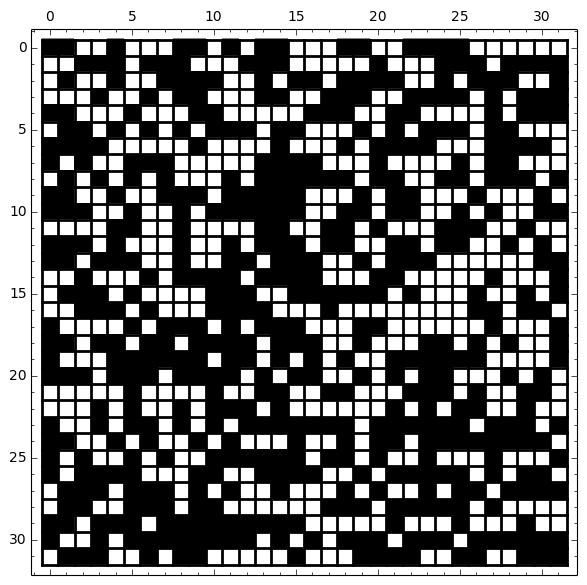
\includegraphics[scale=0.5]{figures/BC_lfsr_ex1.png}
\end{center}
\caption{Visualization of the pseudo-random bit sequence from Figure~\ref{Sage-code-bool-psr},
   generated by SageMath sample~\ref{Sage-code-bool-psr}
   (1 = black, 0 = white)}\label{fig-bool-lfsr2}
\end{figure}
% \clearpage


\subsection{Algebraic Attack on LFSRs}
\label{ss-bool-alg2}
\index{algebraic attack}\index{attack!algebraic}

Even simple random generators\index{random generator} such as LFSRs\index{LFSR}
produce bit sequences that are virtually indistiguishable from true random sequences
by statistical methods, and so provide no hooks for statistical methods of cryptanalysis.
This is not true for attacks with known
plaintext\index{known plaintext}\index{plaintext!known}. The resulting equations
for the key bits are accessible for algebraic
cryptanalysis\index{algebraic cryptanalysis}\index{cryptanalysis!algebraic}. If
the key stream originates from a known source trying to solve these equations
promises success. In particular this holds for LFSRs.

Consider a key bitstream $u_0, u_1, \ldots$ generated by an LFSR\index{LFSR}
by formulas~(\ref{eq-bool-lfsr1}) or (\ref{eq-bool-lfsr2}). Assume a
plaintext $a$ is XOR\index{XOR}\index{encryption!XOR}\index{cipher!XOR}
encrypted using this key stream\index{key stream},
resulting in the ciphertext $c$, where $c_i = a_i + u_i$ for $i = 0, 1, \ldots$
What are the prospects of an attacker who knows a chunk of the plaintext?

Well, assume she knows the first $l+1$ bits\footnote{%
   If she knows any $l+1$ bits, even non-contiguous, the idea of attack
   is the same, only the formalism is slightly more involved.
} of the plaintext. She immediately
derives the corresponding bits $u_0, \ldots, u_l$ of the key stream, in
particular the initial state of the LFSR. For the yet unknown coefficients
$s_i$ she knows a linear relation:
\[
     s_1 u_{l-1} + \cdots + s_l u_0 = u_l.
\]
Each additional known plaintext bit yields one more relation, and having
$l$ relations, from $2l$ bits of known plaintext, the easy linear
algebra\index{linear algebra}\index{algebra!linear} over the field $\F_2$
(in non-degenerate cases) finds a unique solution. In the next subsections
we'll prove, using some deeper mathematical methods:

\begin{theorem}\label{thm-bool-lfsr}
  An LFSR\index{LFSR} of length $l$ is completely predictable from the first $2l$
  bits for the cost of about $\frac{1}{3} \cdot l^3$ bit operations.
\end{theorem}

\subsubsection*{Prediction of LFSRs}

Assume we know the first $2l$ bits $u_0, \ldots, u_{2l-1}$ from an
LFSR\index{LFSR} of length $l$. For an elegant formulation of the linear algebra
methods we introduce the {\bf state vectors\index{state vector}}
\[
     u_{(i)} = (u_i, \ldots, u_{i+l-1}) \quad \text{for } i = 0, 1, \ldots
\]
The vector $u_{(i)}$ is the register content for step $i$ (in reversed order
compared with Figure~\ref{fig-bool-fsr}).
Thus the analysis focusses on the states, not directly on the output. The
recursion~(\ref{eq-bool-lfsr1}) in matrix form (for $n \geq l$) is
\[
     \begin{pmatrix} u_{n-l+1} \\ \vdots \\ u_{n-1} \\ u_{n} \end{pmatrix}
     =
     \begin{pmatrix} 0      & 1      & \ldots & 0      \\
                     \vdots & \vdots & \ddots & \vdots \\
                     0      & 0      & \ldots & 1      \\
                     s_l    & s_{l-1}    & \ldots & s_1 \end{pmatrix}
     \begin{pmatrix} u_{n-l} \\ \vdots \\ u_{n-2} \\ u_{n-1} \end{pmatrix}
\]
or more parsimoniously (the indices being substituted by $m = n-l+1$)
\[
     u_{(m)} = S \cdot u_{(m-1)} \quad \text{for } m \geq 1
\]
where $S$ is the coefficient matrix. As a further step we collect $l$
consecutive state vectors $u_{(i)}, \ldots, u_{(i+l-1)}$ in a state matrix
\[
     U_{(i)} = \begin{pmatrix} u_i      & u_{i+1}      & \ldots & u_{i+l-1}      \\
                               u_{i+1} & u_{i+2} & \ldots & u_{i+l} \\
                               \vdots  & \vdots & \ddots & \vdots     \\
                     u_{i+l-1}    & u_{i+l} & \ldots & u_{2l-2} \end{pmatrix}
\]
and set $U = U_{(0)}$, $V = U_{(1)}$. This gives the formula
\[
     V  =  S \cdot U
\]
that expresses the unknown coefficients $s_1, \ldots, s_l$ by the known
plaintext bits $u_0, \ldots, u_{2l-1}$. Most notably it allows us to write
down the solution immediately---provided that the matrix $U$ is invertible:
\[
     S  =  V \cdot U^{-1}.
\]
The matrix $S$ explicitly displays the coefficients $s_1, \ldots, s_l$.
We'll discuss the invertibility later on.

\subsubsection*{Example}

Assume we are given a ciphertext:
\begin{verbatim}
   10011100 10100100 01010110 10100110 01011101 10101110
   01100101 10000000 00111011 10000010 11011001 11010111
   00110010 11111110 01010011 10000010 10101100 00010010
   11000110 01010101 00001011 11010011 01111011 10110000
   10011111 00100100 00001111 01010011 11111101
\end{verbatim}
We suspect that the cipher is XOR\index{XOR}\index{encryption!XOR}\index{cipher!XOR}
with a key stream from an LFSR of
length $l = 16$. The context suggest that the text is in German and
begins with the word ``Treffpunkt'' (meeting point). To solve the
cryptogram we need 32 bits of plaintext, that is the first four letters
only, presupposed that the theory applies. This gives 32 bits of the
key stream:
\begin{verbatim}
    01010100 01110010 01100101 01100110 = T r e f
    10011100 10100100 01010110 10100110   cipher bits
    -------- -------- -------- --------
    11001000 11010110 00110011 11000000   key bits
\end{verbatim}
SageMath sample~\ref{Sage-code-bool-lfsr2} determines the coefficient matrix.
Its last row tells us that all $s_i = 0$ except $s_{16} = s_5 = s_3 = s_2 = 1$.

Now we know the LFSR and the initial state, and can reconstruct the complete
key stream---yes, it is the same as in Figure~\ref{Sage-code-bool-psr}---and
write down the plaintext (that by the way begins a bit differently from our guess).

\begin{sagecode}
\begin{verbatim}

sage: l = 16
sage: kbits =
      [1,1,0,0,1,0,0,0,1,1,0,1,0,1,1,0,0,0,1,1,0,0,1,1,1,1,0,0,0,0,0,0]
sage: ulist = []
sage: for i in range(0,l):
        state = kbits[i:(l+i)]
        ulist.append(state)
sage: U = matrix(GF(2),ulist)
sage: det(U)
1
sage: W = U.inverse()
sage: vlist = []
sage: for i in range(1,l+1):
        state = kbits[i:(l+i)]
        vlist.append(state)
sage: V = matrix(GF(2),vlist)
sage: S = V*W
sage: S
[0 1 0 0 0 0 0 0 0 0 0 0 0 0 0 0]
[0 0 1 0 0 0 0 0 0 0 0 0 0 0 0 0]
[0 0 0 1 0 0 0 0 0 0 0 0 0 0 0 0]
[0 0 0 0 1 0 0 0 0 0 0 0 0 0 0 0]
[0 0 0 0 0 1 0 0 0 0 0 0 0 0 0 0]
[0 0 0 0 0 0 1 0 0 0 0 0 0 0 0 0]
[0 0 0 0 0 0 0 1 0 0 0 0 0 0 0 0]
[0 0 0 0 0 0 0 0 1 0 0 0 0 0 0 0]
[0 0 0 0 0 0 0 0 0 1 0 0 0 0 0 0]
[0 0 0 0 0 0 0 0 0 0 1 0 0 0 0 0]
[0 0 0 0 0 0 0 0 0 0 0 1 0 0 0 0]
[0 0 0 0 0 0 0 0 0 0 0 0 1 0 0 0]
[0 0 0 0 0 0 0 0 0 0 0 0 0 1 0 0]
[0 0 0 0 0 0 0 0 0 0 0 0 0 0 1 0]
[0 0 0 0 0 0 0 0 0 0 0 0 0 0 0 1]
[1 0 0 0 0 0 0 0 0 0 0 1 0 1 1 0]
\end{verbatim}
\caption{Determining a coefficient matrix}\label{Sage-code-bool-lfsr2}
\end{sagecode}

\subsubsection*{Proof of the Theorem}

We have shown that the cofficients are uniquely determined assuming the
state matrix $U = U_{(0)}$ is invertible. As a consequence in this case
the LFSR is completely known, and all output bits are predictable. We
have yet to discuss the case where the matrix $U$ is singular.

If one of the first $l$ state vectors (= rows of the matrix $U$) is zero,
then all following state vectors are zero too, and prediction is trivial.

Thus we may assume that none of these vectors are zero, but that they are
linearly dependent. Then there is a smallest index $k \geq 1$ such that
$u_{(k)}$ is contained in the subspace spanned by $u_{(0)}, \ldots, u_{(k-1)}$,
and we find coefficients $t_1, \ldots, t_k \in \F_2$ such that
\[
     u_{(k)}  =  t_1 u_{(k-1)} + \cdots + t_k u_{(0)}.
\]
Then also $u_{(k+1)} = S\cdot u_{(k)} = 
t_1 S\cdot u_{(k-1)} + \cdots + t_k S\cdot u_{(0)} =
t_1 u_{(k)} + \cdots + t_k u_{(1)}$, and by induction we get
\[
     u_{(n)}  =  t_1 u_{(n-1)} + \cdots + t_k u_{(n-k)}
     \quad \text{for all } n \geq k.
\]
This formula predicts all the following bits.

The statement on the cost follows from Theorem~\ref{thm-bool-lin}.

\subsubsection*{Discussion}

\begin{itemize}
   \item For a singular state matrix this consideration yields a shorter
      LFSR (of length $k < l$) that generates exactly the same sequence.
      Then our method doesn't determine the coefficients of the original
      register but nevertheless correctly predicts the sequence.
   \item If the bits the attacker knows aren't just the first ones but $2l$
      contiguous ones at a later position, then the theorem yields only the
      prediction of the following bits. In the main case of an invertible
      state matrix $U$ the LFSR is completely known and may be run backwards
      to get the previous bits. For a singular state matrix we achieve
      the same effect using the shorter LFSR constructed above.
   \item The situation where $2l$ bits of the key stream are known but
      at non-contiguous positions is slightly more involved. We get
      linear relations that contain additional (unknown) intermediate bits.
      If $m$ is the number of these then we get $l+m$ linear equations for
      $l+m$ unknown bits.
   \item What if the length $l$ of the LFSR is unknown? Exhaustively trying
      all values $l = 1, 2, 3, \ldots$ is nasty but feasible. A better approach
      is provided by the Berlekamp-Massey\footnote{%
      in SageMath contained as {\tt sage.crypto.lfsr.berlekamp\_massey}, in
      CrypTool\,2 under ``cryptanalysis''/``generic''/``Berlekamp-Massey algorithm''
      } algorithm that is efficient also without knowledge of $l$. We won't
      treat it in this chapter.
\end{itemize}

\subsubsection*{Summary}

Given a random generator\index{random generator} as in Figure~\ref{fig-bool-prg}
cryptanalytic targets are:
\begin{itemize}
\item the secret parameters,
\item the initial state,
\item additional parts of the output (``prediction problem\index{prediction problem}''),
\end{itemize}
given some parts of the output. As we saw for LFSRs\index{LFSR} the prediction
problem has a solution even when the internal parameters remain unknown. Thus:
\begin{quote}
   {\em Cryptanalysis of a random generator first of all means solving the
   prediction problem. A random generator\index{random generator} is
   cryptographically secure if its prediction problem admits no efficient
   solution.}
\end{quote}

\begin{quote}
   {\em Linear feedback shift registers\index{LFSR}\index{feedback shift register!linear}
   are not cryptographically secure.}
\end{quote}


\subsection{Approaches to Nonlinearity\index{nonlinearity} for Feedback Shift
   Registers}\label{ss-bool-nlsr}

LFSRs are popular---in particular among electrical engineers and military---for
several reasons:
\begin{itemize}
	\item very easy implementation,
	\item extreme efficiency in hardware,
	\item good qualification as random generators for statistical applications
         and simulations,
	\item unproblematic operation in parallel even in large quantities.
\end{itemize}
But unfortunately from a cryptological view they are completely insecure if
used naively. To capitalize their positive properties while escaping their
cryptological weakness there are several approaches.

\subsubsection*{Approach 1, Nonlinear Feedback}

Nonlinear feedback\index{feedback} follows the scheme from
Figure~\ref{fig-bool-fsr} with a nonlinear Boolean
function\index{Boolean function}\index{function!Boolean} $f$.
We won't pursue this approach here. We saw a very simple toy
example in SageMath sample~\ref{Sage-code-bool-fsr1}.
There is a general proof that in realistic use cases
NLFSRs\index{NLFSR}\footnote{%
   for Non Linear Feedback Shift Register\index{feedback shift register!nonlinear}
}
are cryptographically useless if used in the direct naive
way \cite{Pom2016}.


\subsubsection*{Approach 2, Nonlinear Output Filter}

The nonlinear ouput filter\index{output filter} (nonlinear feedforward)
realizes the scheme from Figure~\ref{fig-bool-nlf}. The shift register
itself is linear, the Boolean function $f$, nonlinear.

The nonlinear ouput filter is a special case of a nonlinear combiner.

\begin{figure}
\begin{center}
\begin{picture}(320,150)
  \linethickness{2pt}
  \put(20,20){\line(1,0){260}}
  \put(20,20){\line(0,1){30}}
  \put(20,50){\line(1,0){260}}
  \put(280,20){\line(0,1){30}}
  \put(260,120){\circle{30}}
  \put(256,117){$f$}

  \linethickness{1pt}
  \put(60,20){\line(0,1){30}}
  \put(100,20){\line(0,1){30}}
  \put(240,20){\line(0,1){30}}
  \put(200,20){\line(0,1){30}}
  \put(110,30){\ldots}
  \put(180,30){\ldots}

  \put(40,20){\line(0,-1){20}}
  \put(80,20){\line(0,-1){20}}
  \put(220,20){\line(0,-1){20}}
  \put(260,20){\line(0,-1){20}}
  \put(260,0){\line(-1,0){260}}
  \put(0,0){\line(0,1){35}}
  \put(0,35){\vector(1,0){20}}

  \put(260,50){\vector(0,1){53}}
  \put(220,50){\vector(1,2){29}}
  \put(80,50){\line(0,1){25}}
  \put(80,75){\vector(4,1){163}}
  \put(40,50){\line(0,1){70}}
  \put(40,120){\vector(1,0){203}}

  \put(277,120){\vector(1,0){43}}
\end{picture}
\end{center}
\caption{Nonlinear ouput filter for an LFSR}\label{fig-bool-nlf}
\end{figure}

\subsubsection*{Approach 3, Nonlinear Combiner\index{combiner}}

The nonlinear combiner uses a ``battery'' of $n$ LFSRs---preferably
of different lengths---operated in parallel. The output sequences of the LFSRs
serve as input\footnote{%
   hence the occasional denotation ``nonlinear feedforward''
} of a Boolean function\index{Boolean function}\index{function!Boolean}
$f\!\!: \F_2^n \longrightarrow \F_2$, see Figure~\ref{fig-bool-nlc}.
We'll see in Section~\ref{ss-bool-bsana} how to cryptanalyze this
random generator.

\begin{figure}
\begin{center}
\begin{picture}(350,200)
  \linethickness{2pt}
  \put(20,20){\line(1,0){260}}
  \put(20,20){\line(0,1){30}}
  \put(20,50){\line(1,0){260}}
  \put(280,20){\line(0,1){30}}

  \linethickness{1pt}
  \put(60,20){\line(0,1){30}}
  \put(100,20){\line(0,1){30}}
  \put(240,20){\line(0,1){30}}
  \put(200,20){\line(0,1){30}}
  \put(110,30){\ldots}
  \put(180,30){\ldots}

  \put(40,20){\line(0,-1){20}}
  \put(80,20){\line(0,-1){20}}
  \put(220,20){\line(0,-1){20}}
  \put(260,20){\line(0,-1){20}}
  \put(260,0){\line(-1,0){260}}
  \put(0,0){\line(0,1){35}}
  \put(0,35){\vector(1,0){20}}

  \linethickness{2pt}
  \put(20,150){\line(1,0){260}}
  \put(20,150){\line(0,1){30}}
  \put(20,180){\line(1,0){260}}
  \put(280,150){\line(0,1){30}}

  \linethickness{1pt}
  \put(60,150){\line(0,1){30}}
  \put(100,150){\line(0,1){30}}
  \put(240,150){\line(0,1){30}}
  \put(200,150){\line(0,1){30}}
  \put(110,160){\ldots}
  \put(180,160){\ldots}

  \put(40,150){\line(0,-1){20}}
  \put(80,150){\line(0,-1){20}}
  \put(220,150){\line(0,-1){20}}
  \put(260,150){\line(0,-1){20}}
  \put(260,130){\line(-1,0){260}}
  \put(0,130){\line(0,1){35}}
  \put(0,165){\vector(1,0){20}}

  \put(80,100){$\vdots$}
  \put(220,100){$\vdots$}
  \put(80,70){$\vdots$}
  \put(220,70){$\vdots$}

  \put(280,165){\vector(1,0){20}}
  \put(280,35){\vector(1,0){20}}
  \put(315,100){\oval(30,160)}
  \put(330,100){\vector(1,0){20}}
  \put(313,97){$f$}
\end{picture}
\end{center}
\caption{Nonlinear combiner}\label{fig-bool-nlc}
\end{figure}

\subsubsection*{Approach 4, Output Selection/Decimation/Clocking}

There are different ways of controlling a battery of $n$ parallel LFSRs
by another LFSR:
\begin{itemize}
   \item {\bf Output selection}\index{output selection} takes the current
      output bit of exactly one of the LFSRs from the ``battery'', depending
      on the state of the auxiliary register, and outputs it as the next
	 pseudo-random bit. More generally we could choose ``$r$ from $n$''.
   \item For {\bf decimation}\index{decimation} one usually takes $n = 1$,
      and outputs the current bit of the one battery register only if the
	 auxiliary register is in a certain state, for example its own current
      output is $1$. Of course this kind of decimation
	 applies to arbitrary bit sequences in an analogous way.
   \item For {\bf clocking}\index{clocking} we look at the state of the
      auxiliary register and depending on it decide which of the battery
	 registers to step in the current cycle (and by how many positions),
      leaving the other registers in their current states\footnote{%
	   This reminds of the control logic of rotor machines\index{rotor machine}
        in classical cryptography.
        }.
\end{itemize}
These methods turn out to be special cases of nonlinear combiners if
properly rewritten. Thus approach 3 represents the most important method of
making the best of LFSRs\index{LFSR}.

The encryption standard \href{https://en.wikipedia.org/wiki/A5/1}{A5/1}\index{A5}
for mobile communications uses three LFSRs of lengths 19, 22 und 23, each
with maximum possible period, and slightly differently clocked. It linearly
(by simple binary addition) combines the three output streams. The---even
weaker---algorithm A5/2 controls the clocking by an auxiliary register.
Both variants can be broken on a standard PC in real-time.

The Bluetooth encryption standard $\mathrm{E}_0$\index{E0} uses four LFSRs
and combines them in a nonlinear way. This method is somewhat stronger than
A5, but also too weak for real security \cite{Schm2003}.

\subsubsection*{Example: The Geffe Generator}

The Geffe generator\index{Geffe generator} provides a simple example of
output selection. Its description is in Figure~\ref{fig-bool-gef}.
The output is $x$, if $z = 0$, and $y$, if $z = 1$. Expressed by a formula:
\begin{eqnarray*}
   u & = & \begin{cases}
              x, & \text{if } z = 0, \\
              y, & \text{if } z = 1
           \end{cases} \\
      & = & (1 - z) x + zy = x + zx + zy.
\end{eqnarray*}
This formula shows how to interpret the Geffe generator as a nonlinear
combiner with a Boolean function $f\!\!: \F_2^3 \longrightarrow \F_2$ of degree 2.
For later use we implement $f$ in SageMath sample~\ref{Sage-code-bool-gef}.

\begin{figure}
\begin{center}
\setlength{\unitlength}{1pt}
\begin{picture}(350,200)
  \linethickness{2pt}
  \put(20,20){\line(1,0){260}}
  \put(20,20){\line(0,1){30}}
  \put(20,50){\line(1,0){260}}
  \put(280,20){\line(0,1){30}}

  \linethickness{1pt}
  \put(60,20){\line(0,1){30}}
  \put(100,20){\line(0,1){30}}
  \put(240,20){\line(0,1){30}}
  \put(200,20){\line(0,1){30}}
  \put(110,30){\ldots}
  \put(180,30){\ldots}

  \put(40,20){\line(0,-1){20}}
  \put(80,20){\line(0,-1){20}}
  \put(220,20){\line(0,-1){20}}
  \put(260,20){\line(0,-1){20}}
  \put(260,0){\line(-1,0){260}}
  \put(0,0){\line(0,1){35}}
  \put(0,35){\vector(1,0){20}}

  \linethickness{2pt}
  \put(20,80){\line(1,0){260}}
  \put(20,80){\line(0,1){30}}
  \put(20,110){\line(1,0){260}}
  \put(280,80){\line(0,1){30}}

  \linethickness{1pt}
  \put(60,80){\line(0,1){30}}
  \put(100,80){\line(0,1){30}}
  \put(240,80){\line(0,1){30}}
  \put(200,80){\line(0,1){30}}
  \put(110,90){\ldots}
  \put(180,90){\ldots}

  \put(40,80){\line(0,-1){20}}
  \put(80,80){\line(0,-1){20}}
  \put(220,80){\line(0,-1){20}}
  \put(260,80){\line(0,-1){20}}
  \put(260,60){\line(-1,0){260}}
  \put(0,60){\line(0,1){35}}
  \put(0,95){\vector(1,0){20}}

  \linethickness{2pt}
  \put(50,160){\line(1,0){260}}
  \put(50,160){\line(0,1){30}}
  \put(50,190){\line(1,0){260}}
  \put(310,160){\line(0,1){30}}

  \linethickness{1pt}
  \put(90,160){\line(0,1){30}}
  \put(130,160){\line(0,1){30}}
  \put(270,160){\line(0,1){30}}
  \put(230,160){\line(0,1){30}}
  \put(140,170){\ldots}
  \put(210,170){\ldots}

  \put(70,160){\line(0,-1){20}}
  \put(110,160){\line(0,-1){20}}
  \put(250,160){\line(0,-1){20}}
  \put(290,160){\line(0,-1){20}}
  \put(290,140){\line(-1,0){260}}
  \put(30,140){\line(0,1){35}}
  \put(30,175){\vector(1,0){20}}

  \put(310,175){\line(1,0){20}}
  \put(330,175){\line(0,-1){40}}
  \put(333,152){$z$}
  \put(330,135){\line(-1,0){15}}
  \put(315,135){\vector(0,-1){25}}

  \put(280,95){\vector(1,0){20}}
  \put(288,97){$x$}
  \put(280,35){\vector(1,0){20}}
  \put(288,38){$y$}
  \put(315,65){\oval(30,90)}
  \put(330,65){\line(-1,-1){30}}
  \put(330,65){\vector(1,0){20}}
\end{picture}
\end{center}
\caption{Geffe generator}\label{fig-bool-gef}
\end{figure}

\begin{sagecode}
\begin{verbatim}

sage: geff = BoolF(str2bbl("00011100"),method="ANF")
sage: geff.printTT()
Value at 000 is 0
Value at 001 is 0
Value at 010 is 0
Value at 011 is 1
Value at 100 is 1
Value at 101 is 0
Value at 110 is 1
Value at 111 is 1
\end{verbatim}
\caption{The Geffe function}\label{Sage-code-bool-gef}
\end{sagecode}

\subsection{Implementation of a Nonlinear Combiner}\label{ss-bool-ncsr}

A nonlinear combiner\index{combiner} uses several LFSRs, operated in parallel.
This suggests an implementation of LFSRs as objects of a class {\tt LFSR}\footnote{%
   see also CrypTool\,2, ``protocols''/``LFSR'' or ``NLFSR''
}.
\newpage

\begin{description}
   \item[Class {\tt LSFR}:] ~
      \begin{description}
         \item[Attributes:] ~
            \begin{itemize}
               \item {\tt length}: the length of the register
               \item {\tt taplist} (constant): the list of coefficients (or taps)
                  that define the bits for feedback
               \item {\tt state} (variable): the state of the register
            \end{itemize}
         \item[Methods:] ~
            \begin{itemize}
               \item {\tt setLength}: define the length (used only implicitly
                  for initialization)
               \item {\tt setTaps}: define the list of taps (used only implicitly
                  for initialization)
               \item {\tt setState}: set the state of the register
               \item {\tt getLength}: output the length
               \item {\tt nextBits}: generate a given number of output bits,
                  and set the next state
            \end{itemize}
      \end{description}
\end{description}
For observing the register a method (generically called {\tt \_\_str\_\_}
in Python) is convenient that outputs the attributes in human-readable form.

The complete implementation is in SageMath sample~\ref{Sage-code-bool-lfsr3}
in Section~\ref{ss-bool-lfsrclass}.

\subsubsection*{Example: Geffe Generator\index{Geffe generator}}

First we choose\footnote{%
  using the lists of primitive polynomials from \cite{Menezes2001}
} three LFSRs of lengths 15, 16, 17,
whose periods are $2^{15} - 1 = 32767$, $2^{16} - 1 = 65535$, and
$2^{17} - 1 = 131071$. These are pairwise coprime, see SageMath
sample~\ref{Sage-code-bool-per}. Combining their outputs (in each step)
as bitblocks of length $3$ yields a sequence with a period that has an
impressive length of $281459944554495$, about $300 \times 10^{12}$
(300 billions\footnote{%
  European billions. For Americans this are 300 trillions.
}).
SageMath sample~\ref{Sage-code-bool-regs} defines the three LFSRs. The recursive
formula for the third one, the control register {\tt reg17}, is
$u_n = u_{n-3} + u_{n-17}$, since exactly the taps 3 and 17 are ``active''.
We let each of the LFSRs generate a sequence of length 100, see SageMath
sample~\ref{Sage-code-bool-seqs}. The Geffe function combines them in
SageMath sample~\ref{Sage-code-bool-gef-seq}.

\begin{sagecode}
\begin{verbatim}

sage: n15 = 2**15 - 1; n15
32767
sage: n15.factor()
7 * 31 * 151
sage: n16 = 2**16 - 1; n16
65535
sage: n16.factor()
3 * 5 * 17 * 257
sage: n17 = 2**17 - 1; n17
131071
sage: n17.factor()
131071
sage: period = n15 * n16 * n17; period
281459944554495
\end{verbatim}
\caption{Calculating a period}\label{Sage-code-bool-per}
\end{sagecode}

\begin{sagecode}
\begin{verbatim}

sage: reg15 = LFSR([1,0,0,0,0,0,0,0,0,0,0,0,0,0,1])
sage: reg15.setState([0,1,1,0,1,0,1,1,0,0,0,1,0,0,1])
sage: print(reg15)
Length: 15 | Taps: 100000000000001 | State: 011010110001001
sage: reg16 = LFSR([0,1,1,0,1,0,0,0,0,0,0,0,0,0,0,1])
sage: reg16.setState([0,1,1,0,1,0,1,1,0,0,0,1,0,0,1,1])
sage: print(reg16)
Length: 16 | Taps: 0110100000000001 | State: 0110101100010011
sage: reg17 = LFSR([0,0,1,0,0,0,0,0,0,0,0,0,0,0,0,0,1])
sage: reg17.setState([0,1,1,0,1,0,1,1,0,0,0,1,0,0,1,1,1])
sage: print(reg17)
Length: 17 | Taps: 00100000000000001 | State: 01101011000100111
\end{verbatim}
\caption{Three LFSRs}\label{Sage-code-bool-regs}
\end{sagecode}

\begin{sagecode}
\begin{verbatim}

sage: nofBits = 100
sage: outlist15 = reg15.nextBits(nofBits)
sage: print(outlist15)
[1, 0, 0, 1, 0, 0, 0, 1, 1, 0, 1, 0, 1, 1, 0, 1, 1, 1, 0, 0,
 0, 0, 1, 0, 0, 1, 1, 0, 1, 1, 0, 1, 0, 0, 0, 0, 0, 1, 1, 1,
 0, 1, 1, 0, 1, 1, 0, 0, 0, 0, 0, 0, 1, 0, 1, 1, 0, 1, 1, 0,
 1, 1, 1, 1, 1, 1, 1, 0, 0, 1, 0, 0, 1, 0, 0, 1, 0, 1, 0, 1,
 0, 1, 1, 1, 0, 0, 0, 1, 1, 1, 0, 0, 1, 1, 0, 0, 1, 0, 1, 1]
sage: outlist16 = reg16.nextBits(nofBits)
sage: print(outlist16)
[1, 1, 0, 0, 1, 0, 0, 0, 1, 1, 0, 1, 0, 1, 1, 0, 0, 0, 1, 1,
 0, 0, 1, 1, 1, 1, 0, 0, 0, 0, 0, 0, 0, 0, 1, 1, 1, 0, 1, 1,
 1, 0, 0, 0, 1, 1, 1, 0, 0, 0, 0, 0, 1, 0, 0, 0, 1, 1, 1, 0,
 1, 1, 1, 1, 0, 1, 0, 0, 1, 0, 0, 1, 1, 1, 1, 0, 0, 1, 0, 1,
 1, 0, 1, 1, 1, 1, 0, 0, 1, 0, 1, 1, 1, 0, 0, 1, 0, 0, 0, 1]
sage: outlist17 = reg17.nextBits(nofBits)
sage: print(outlist17)
[1, 1, 1, 0, 0, 1, 0, 0, 0, 1, 1, 0, 1, 0, 1, 1, 0, 0, 0, 1,
 0, 0, 0, 0, 0, 0, 1, 1, 0, 0, 1, 1, 1, 1, 1, 1, 0, 1, 1, 0,
 1, 1, 0, 0, 0, 0, 0, 1, 1, 1, 0, 0, 0, 0, 1, 1, 0, 0, 0, 0,
 0, 0, 0, 0, 1, 1, 1, 1, 1, 1, 1, 0, 0, 1, 0, 0, 1, 0, 0, 1,
 0, 1, 0, 1, 0, 1, 0, 1, 1, 0, 0, 1, 0, 1, 1, 0, 0, 1, 1, 0]
\end{verbatim}
\caption{Three LFSR sequences}\label{Sage-code-bool-seqs}
\end{sagecode}
\clearpage

\begin{sagecode}
\begin{verbatim}

sage: outlist = []
sage: for i in range(0,nofBits):
....:     x = [outlist15[i],outlist16[i],outlist17[i]]
....:     outlist.append(geff.valueAt(x))
....: 
sage: print(outlist)
[1, 1, 0, 1, 0, 0, 0, 1, 1, 1, 0, 0, 0, 1, 1, 0, 1, 1, 0, 1,
 0, 0, 1, 0, 0, 1, 0, 0, 1, 1, 0, 0, 0, 0, 1, 1, 0, 0, 1, 1,
 1, 0, 1, 0, 1, 1, 0, 0, 0, 0, 0, 0, 1, 0, 0, 0, 0, 1, 1, 0,
 1, 1, 1, 1, 0, 1, 0, 0, 1, 0, 0, 0, 1, 1, 0, 1, 0, 1, 0, 1,
 0, 0, 1, 1, 0, 1, 0, 0, 1, 1, 0, 1, 1, 0, 0, 0, 1, 0, 0, 1]
\end{verbatim}
\caption{The combined sequence}\label{Sage-code-bool-gef-seq}
\end{sagecode}

\subsection{Correlation Attacks\index{correlation attack}---the
   Achilles Heels of Combiners}\label{ss-bool-bsana}

Let $f\!\!: \F_2^n \longrightarrow \F_2$ be the combining function of a
nonlinear combiner\index{combiner}. The number
\[
   K_f := \#\{ x = (x_1, \ldots, x_n) \in \F_2^n \:|\: f(x) = x_1 \}
\]
counts the coincidences of the value of the function with its first argument.
If it is $> 2^{n-1}$, then the probability of a coincidence,
\[
   p = \frac{1}{2^n} \cdot K_f > \frac{1}{2},
\]
is above average, and the combined output sequence ``correlates'' with the
output of the first LFSR more then expected by random. If $p < \frac{1}{2}$,
then the correlation deviates from the expected value in the other direction.

The cryptanalyst can exploit this effect in an attack with known
plaintext\index{known plaintext}\index{plaintext!known}. We suppose that
she knows the ``hardware'', that is the taps of the registers, and also
the combining function $f$. She seeks the initial states of all the LFSRs.
We assume she knows the bits $k_0, \ldots, k_{r-1}$ of the key stream\footnote{%
  for simplicity of exposition the first ones. The argument works in the
  same way for any $r$ known key bits.
}. For each of the $2^{l_1}$ initial states of the first LFSR she generates
the sequence $u_0, \ldots, u_{r-1}$, and counts the coincidences. The expected
values are
\[
   \frac{1}{r}\cdot \#\{i \:|\: u_i = k_i\} \approx
   \begin{cases}
      p & \text{for the correct initial state of LFSR 1,} \\
      \frac{1}{2} & \text{otherwise.}
   \end{cases}
\]
If $r$ is large enough, she can determine the true initial state of LFSR 1
(with high probability) for a cost of $\sim 2^{l_1}$. She continues with
the other registers, and finally identifies the complete key with a cost
of $\sim 2^{l_1} + \cdots + 2^{l_n}$. Note that the cost is exponential,
but significantly lower than the cost $\sim 2^{l_1} \cdots 2^{l_n}$ of the
naive exhaustion of the key space.

In the language of linear
cryptanalysis\index{linear cryptanalysis}\index{cryptanalysis!linear}
from \ref{ss-bool-lka} she made use of the linear
relation\index{linear relation}\index{relation!linear}
\[
     f(x_1, \ldots, x_n) \stackrel{p}{\approx} x_1
\]
for $f$. Clearly she could use any linear relation as well to reduce the
complexity of key search\footnote{%
  A more in-depth analysis of the situation leads to the notion of
  correlation immunity\index{correlation immunity} that is related with
  the linear potential\index{linear potential}\index{potential!linear}.
}.

\subsubsection*{Correlations from the Geffe Generator}

From the truth table~\ref{tab-bool-gef-wt} we get the correlations produced by
the Geffe generator\index{Geffe generator}. Thus the probabilities of
coincidences are
\[
   p = \begin{cases}
          \frac{3}{4} & \text{for register 1 ($x$),} \\
          \frac{3}{4} & \text{for register 2 ($y$),} \\
          \frac{1}{2} & \text{for register 3 ($z =$ control bit).}
       \end{cases}
\]
A correlation attack easily detects the initial states of registers
1 and 2---the battery registers---given only a short piece of an output
sequence. Afterwards exhaustion finds the initial state of register 3,
the control register.

\begin{table}[h]
\begin{center}
  \begin{tabular}{|c|cccc|cccc|}\hline
      $x$    & $0$ & $0$ & $0$ & $0$ & $1$ & $1$ & $1$ & $1$ \\
      $y$    & $0$ & $0$ & $1$ & $1$ & $0$ & $0$ & $1$ & $1$ \\
      $z$    & $0$ & $1$ & $0$ & $1$ & $0$ & $1$ & $0$ & $1$ \\
    \hline
  $f(x,y,z)$ & $0$ & $0$ & $0$ & $1$ & $1$ & $1$ & $0$ & $1$ \\
    \hline
  \end{tabular}
\end{center}
\caption{Truth table of the Geffe function (in horizontal order)}\label{tab-bool-gef-wt}
\end{table}

We exploit this weakness of the Geffe generator in SageMath
sample~\ref{Sage-code-bool-gef-lp} that continues SageMath
sample~\ref{Sage-code-bool-gef}. Since we defined the linear
profile\index{linear profile}\index{profile!linear} for objects of the
class {\tt BoolMap} only, we first of all have to interpret the
function {\tt geff} as a Boolean map, that is a one-element list of
Boolean functions. Then the linear profile is represented by a matrix
of 2 columns and 8 rows. The first column {\tt [64, 0, 0, 0, 0, 0, 0, 0]}
shows the coincidences with the linear form 0 in the range. So it contains
no useful information, except the denominator $64$ that applies to all
entries. The second row {\tt [0, 0, 16, 16, 16, 16, 0, 0]} yields the
list of coincidence probabilities $p$ (after dividing it by $64$)
in Table~\ref{tab-bool-gef-korr}, using the formula
\[
     p = \frac{1}{2} \cdot (\pm \sqrt{\lambda} + 1).
\]

If $\lambda = 0$, then $p = 1/2$. If  $\lambda = 1/4$, then $p = 1/4$
or $3/4$. For deciding between these two values for $p$ we use
Table~\ref{tab-bool-gef-wt}.

\begin{table}[h]
\begin{center}
\begin{tabular}{|l|cccccccc|} \hline
  linear form     & $0$   &   $z$   &   $y$    &   $y+z$   &  $x$    &   $x+z$   &  $x+y$  & $x+y+z$ \\
  representation  & $000$ & $001$ & $010$ & $011$ & $100$ & $101$ & $110$ & $111$ \\ \hline
  potential       & $0$   & $0$   & $1/4$ & $1/4$ & $1/4$ & $1/4$ & $0$   & $0$ \\
  probability $p$ & $1/2$ & $1/2$ & $3/4$ & $1/4$ & $3/4$ & $3/4$ & $1/2$ & $1/2$ \\ \hline
\end{tabular}
\end{center}
\caption{Coincidence probabilities of the Geffe function}\label{tab-bool-gef-korr}
\end{table}

\begin{sagecode}
\begin{verbatim}

sage: g = BoolMap([geff])
sage: linProf = g.linProf(); linProf
[[64,0], [0,0], [0,16], [0,16], [0,16], [0,16], [0,0], [0,0]]
\end{verbatim}
\caption{Linear profile of the Geffe function}\label{Sage-code-bool-gef-lp}
\end{sagecode}

In SageMath sample~\ref{Sage-code-bool-gef-coi} we apply this finding to the
$100$ element sequence from SageMath sample~\ref{Sage-code-bool-gef-seq}.
The function {\tt coinc} from SageMath sample~\ref{Sage-code-bool-div-bbl}
(in the appendix) counts the coincidences. For the first register we
find $73$ coincidences, for the second one $76$, for the third one
only $41$. This confirms the values $75$, $75$, $50$ predicted by our theory
(taking into account statistical variability).

\begin{sagecode}
\begin{verbatim}

sage: coinc(outlist15,outlist)
73
sage: coinc(outlist16,outlist)
76
sage: coinc(outlist17,outlist)
41
\end{verbatim}
\caption{Coincidences for the Geffe generator}\label{Sage-code-bool-gef-coi}
\end{sagecode}

\subsubsection*{Cryptanalysis of the Geffe Generator\index{Geffe generator}}

These results promise an effortless analysis of our sample sequence. For an
assessment of the success probability
we consider a bitblock $b \in \F_2^r$ and first ask how large is the
probability that a random bitblock $u \in \F_2^r$ coincides with $b$ at
exactly $t$ positions. For an answer we have to look at the symmetric binomial
distribution\index{binomial distribution} (where $p = \frac{1}{2}$ is
the probability of coincidence at a single position): The probability of
exactly $t$ coincidences is
\[
     B_{r,\frac{1}{2}}(t)  =  \frac{\binom{r}{t}}{2^r}.
\]
Hence the cumulated probability of up to $T$ coincidences is
\[
     \sum_{t=0}^T B_{r,\frac{1}{2}}(t)
       =  \frac{1}{2^r} \cdot \sum_{t=0}^T \binom{r}{t}.
\]
If $r$ is not too large, then we may explicitly calculate this value
for a given bound $T$. If on the other hand $r$ is not too small, then
we approximate the value using the normal distribution\index{normal distribution}.
The mean value of the number of coincidences is $r/2$, the variance, $r/4$,
and the standard deviation, $\sqrt{r}/2$.

In any case for $r = 100$ the probability of finding at most (say) $65$
coincidences is $0.999$, the probability of surpassing this number
is 1\,\permil. For the initial state of register 1 we have to
try $2^{15} = 32786$ possibilities (generously including the zero
state $0 \in \F_2^{15}$ into the count). So we expect about $33$
oversteppings with at least $66$ coincidences. One of these should
occur for the true initial state of register 1 that we expect to produce
about $75$ coincidences. Maybe it even produces the maximum number
of coincidences.

\begin{sagecode}
\begin{verbatim}

sage: clist = []
sage: histogr = [0] * (nofBits + 1)
sage: for i in range(0,2**15):
....:     start = int2bbl(i,15)
....:     reg15.setState(start)
....:     testlist = reg15.nextBits(nofBits)
....:     c = coinc(outlist,testlist)
....:     histogr[c] += 1
....:     clist.append(c)
....:     
sage: print(histogr)
[0, 0, 0, 0, 0, 0, 0, 0, 0, 0, 0, 0, 0, 0, 0, 0, 0, 0, 0, 0, 0,
 0, 0, 0, 0, 0, 0, 0, 0, 0, 0, 0, 0, 4, 12, 12, 37, 78, 116, 216,
 329, 472, 722, 1003, 1369, 1746, 1976, 2266, 2472, 2531, 2600,
 2483, 2355, 2149, 1836, 1574, 1218, 928, 726, 521, 343, 228, 164,
 102, 60, 47, 36, 13, 8, 7, 4, 2, 1, 2, 0, 0, 0, 0, 0, 0, 0, 0, 0,
 0, 0, 0, 0, 0, 0, 0, 0, 0, 0, 0, 0, 0, 0, 0, 0, 0, 0]
sage: mm = max(clist)
sage: ix = clist.index(mm)
sage: block = int2bbl(ix,15)
sage: print "Maximum =", mm, "at index", ix, ", start value", block
Maximum = 73 at index 13705 , start value\
 [0, 1, 1, 0, 1, 0, 1, 1, 0, 0, 0, 1, 0, 0, 1]
\end{verbatim}
\caption{Analysis of the Geffe generator---register 1}\label{Sage-code-bool-gef-ana1}
\end{sagecode}

SageMath sample~\ref{Sage-code-bool-gef-ana1} shows that this really
happens. However the maximum number of coincidences, $73$, occurs
twice in the histogram. The first occurrence happens at index
$13705$, corresponding to the initial state $011010110001001$,
the correct solution. The second occurrence, at index $31115$, see SageMath
sample~\ref{Sage-code-bool-gef-ana1a}, yields the false solution
$111100110001011$ that eventually leads to a contradiction.

\begin{sagecode}
\begin{verbatim}

sage: ix = clist.index(mm,13706); ix
31115
sage: print int2bbl(ix,15)
[1, 1, 1, 1, 0, 0, 1, 1, 0, 0, 0, 1, 0, 1, 1]
\end{verbatim}
\caption{Analysis of the Geffe generator---continued}\label{Sage-code-bool-gef-ana1a}
\end{sagecode}

SageMath sample~\ref{Sage-code-bool-gef-ana2} shows the analogous analysis
of register 2. Here the maximum of coincidences, $76$, is unique,
occurs at index $27411$ corresponding to the initial state $0110101100010011$,
and provides the correct solution.

\begin{sagecode}
\begin{verbatim}

sage: clist = []
sage: histogr = [0] * (nofBits + 1)
sage: for i in range(0,2**16):
....:     start = int2bbl(i,16)
....:     reg16.setState(start)
....:     testlist = reg16.nextBits(nofBits)
....:     c = coinc(outlist,testlist)
....:     histogr[c] += 1
....:     clist.append(c)
....:     
sage: print(histogr)
[0, 0, 0, 0, 0, 0, 0, 0, 0, 0, 0, 0, 0, 0, 0, 0, 0, 0, 0, 0,
 0, 0, 0, 0, 0, 0, 0, 1, 0, 2, 3, 4, 8, 17, 25, 51, 92, 171,
 309, 477, 750, 1014, 1423, 1977, 2578, 3174, 3721, 4452, 4821,
 5061, 5215, 5074, 4882, 4344, 3797, 3228, 2602, 1974, 1419,
 1054, 669, 434, 306, 174, 99, 62, 38, 19, 10, 3, 0, 1, 0, 0,
 0, 0, 1, 0, 0, 0, 0, 0, 0, 0, 0, 0, 0, 0, 0, 0, 0, 0, 0, 0,
 0, 0, 0, 0, 0, 0, 0]
sage: mm = max(clist)
sage: ix = clist.index(mm)
sage: block = int2bbl(ix,16)
sage: print "Maximum =", mm, "at index", ix, ", start value", block
Maximum = 76 at index 27411 , start value\
 [0, 1, 1, 0, 1, 0, 1, 1, 0, 0, 0, 1, 0, 0, 1, 1]
\end{verbatim}
\caption{Analysis of the Geffe generator---register 2}\label{Sage-code-bool-gef-ana2}
\end{sagecode}

To complete the analysis we must yet determine the initial state of register 3,
the control register. The obvious idea is to exhaust the $2^{17}$ different
possibilities. There is a shortcut since we already know $51$ of the first
$100$ bits of the control register: At a position where the values of registers
1 and 2 differ, the control bit is necessarily 0 if the final output coincides
with register 1, and 1 otherwise. Only at positions where registers 1 and 2
coincide the corresponding bit of register 3 is undetermined.
\begin{verbatim}
 register 1: 10010001101011011100001001101101000001110110110000
 register 2: 11001000110101100011001111000000001110111000111000
 register 3: -1-00--0-1101-110001---00-1-00-1--1101--110---0---
bitsequence: 11010001110001101101001001001100001100111010110000

        ... 00101101101111111001001001010101110001110011001011
        ... 00100011101111010010011110010110111100101110010001
        ... ----110-------1-1-11-0-100----01--01-1-001-1-00-1-
        ... 00100001101111010010001101010100110100110110001001
\end{verbatim}
In particular we already know 11 of the 17 initial bits, and are left with only
$2^6 = 64$ possibilities to try.

But even this may be further simplified, since the known and the unknown
bits obey linear relations of the type $u_n = u_{n-3} + u_{n-17}$.
The unknown bits of the initial state are $u_0$, $u_2$, $u_5$, $u_6$, $u_8$,
$u_{13}$. The solution follows the columns of Table~\ref{tab-bool-gef_ana3},
that immediately give
\[
     u_0 = 1,\: u_2 = 1,\: u_6 = 0.
\]
The remaining solutions are
\[
    u_8 = u_{22} = u_{39} = 0,\: u_5 = u_{22} + 1 = u_8 + 1 = 1,\:
    u_{13} = u_{30} + 1 = 0.
\]
Hence the initial state of the control register is {\tt 01101011000100111},
and we know this is the correct solution. We don't need to bother with the
second possible solution for register 1 since we already found a constellation
that correctly reproduces the sequence.

\begin{table}
\begin{center}
\begin{tabular}{c|c|c|c}
   $u_{17}=u_{14}+u_0$    & $0=1+u_0$              & $u_0=1$                &                   \\
   $u_{19}=u_{16}+u_2$    & $1=0+u_2$              & $u_2=1$                &                   \\
   $u_{20}=u_{17}+u_3$    & $u_{20}=0+0$           & $u_{20}=0$             &                   \\
   $u_{22}=u_{19}+u_5$    & $u_{22}=u_5+1$         & $u_5=u_{22}+1$         &                   \\
   $u_{23}=u_{20}+u_6$    & $0=u_{20}+u_6$         & $u_6=u_{20}$           & $u_6=0$           \\
   $u_{25}=u_{22}+u_8$    & $u_{25}=u_{22}+u_8$    & $u_8=u_{22}+u_{25}$    & $u_8=u_{22}$      \\
   $u_{27}=u_{24}+u_{10}$ & $u_{27}=0+1$           & $u_{27}=1$             &                   \\
   $u_{28}=u_{25}+u_{11}$ & $0=u_{25}+0$           & $u_{25}=0$             &                   \\
   $u_{30}=u_{27}+u_{13}$ & $u_{30}=u_{27}+u_{13}$ & $u_{13}=u_{27}+u_{30}$ & $u_{13}=u_{30}+1$ \\
   $u_{33}=u_{30}+u_{16}$ & $u_{33}=u_{30}+0$      & $u_{30}=u_{33}$        & $u_{30}=1$        \\
   $u_{36}=u_{33}+u_{19}$ & $0=u_{33}+1$           & $u_{33}=1$             &                   \\
   $u_{39}=u_{36}+u_{22}$ & $u_{39}=0+u_{22}$      & $u_{22}=u_{39}$        &                   \\
   $u_{42}=u_{39}+u_{25}$ & $0=u_{39}+u_{25}$      & $u_{39}=u_{25}$        & $u_{39}=0$
\end{tabular}
\end{center}
\caption{Determination of the control register's initial state}\label{tab-bool-gef_ana3}
\end{table}

\subsection{Design Criteria for Nonlinear Combiners}

From the forgoing discussion we derive design criteria for nonlinear
combiners\index{combiner}:
\begin{itemize}
	\item The battery registers should be as long as possible.
	\item The combining function $f$ should have a low linear
        potential\index{linear potential}\index{potential!linear}.
\end{itemize}
How long should the battery registers be? There are some algorithms for
``fast'' correlation attacks using the Walsh
transformation\index{Walsh transformation}, in particular against sparse
linear feedback functions (that use only a small number of taps) \cite{MeSt1989}. These
don't reduce the complexity class of the attack (``exponential in the
length of the shortest register'') but reduce the cost by a significant
factor. So they are able to attack registers whose feedback functions have
up to $100$ monomials with coefficients in their ANF. As a consequence
\begin{itemize}
	\item The single LFSRs should have a length of at least 200 bits,
	   and use about $100$ taps each.
\end{itemize}
To assess the number $n$ of LFSRs we bear in mind that the combining
function should be ``correlation immune'', in particular have a low linear
potential. A well-chosen Boolean function of $16$ variables should
suffice\footnote{%
  There are no known recommendations in the literature.
}.

Rueppel\footnote{%
   Rainer A. Rueppel, Swiss cryptographer
} found an elegant way out to make the correlation attack break
down: Use a ``time-dependent'' combining function, that is a family
$(f_t)_{t \in \N}$. The bit $u_t$ of the key stream is calculated by the 
function $f_t$. We won't analyze this approach here.

Observing that the correlation attack needs knowledge of the taps, the
security could be somewhat better if the taps are secret. Then the attacker
has to perform additional exhaustions that multiply the complexity by factors
such as $2^{l_1}$ for the first LFSR alone. This scenario allows choosing LFSRs
of somewhat smaller lengths. But bear in mind that for a hardware
implementation the taps are parts of the algorithm, not of the key,
that is they are public parameters in the sense of Figure ~\ref{fig-bool-prg}.

\subsubsection*{Efficiency}

LFSRs\index{LFSR} and nonlinear combiners\index{combiner} allow efficient
realizations by special hardware that produces one bit per clock cycle. This
rate can be enlarged by parallelization. From this point of view estimating
the cost of execution on a usual PC processor is somewhat inadequate.
Splitting each of the $\geq 200$ bit registers into $4$ parts of about $64$ bits
shifting a single register requires at least 4 clock cycles, summing up to
$64$ clock cycles for $16$ registers. Add some clock cycles for the combining
function. Thus one single bit would take about $100$ clock cycles. A
2-GHz processor, even with optimized implementation, would produce at most
$2 \cdot 10^9 / 100 = 20$ million bits per second.

As a summary we note:
\begin{quote}
  {\em Using LFSRs and nonlinear combining functions we can build useful
  and fast random generators\index{random generator}, especially in hardware.}
\end{quote}

Unfortunately there is no satisfying theory for the cryptologic security of
this type of random generators, even less a mathematical proof. Security is
assessed by plausible criteria that---as for bitblock ciphers---are related
to the nonlinearity\index{nonlinearity} of Boolean
functions\index{Boolean function}\index{function!Boolean}.

\subsection{Perfect (Pseudo-)Random Generators}\label{ss-bool-rndperf}

As we saw the essential cryptologic criterion for random\index{random generator}
generators is unpredictability\index{unpredictable}. In the 1980s cryptographers,
guided by an analogy with asymmetric cryptography, found a way of modelling this
property in terms of complexity theory\index{complexity theory}:
Prediction should boil down
to a known ``hard'' algorithmic problem such as factoring\index{factoring}
or discrete\index{discrete logarithm}\index{logarithm!discrete}
logarithm. This idea established a new quality standard for random generators,
much stronger than statistical tests, but eventually building on unproven
mathematical hypotheses. Thus the situation with respect to the security
of random generators is comparable to asymmetric encryption.

As an interesting twist it soon turned out that in a certain sense
unpredictability is a universal property: For an unpredictable sequence there
is {\em no efficient algorithm at all} that distinguishes it from a true random
sequence, a seemingly much stronger requirement. See Theorem~\ref{thm-bool-YaoTh}
(Yao's theorem). This universality justifies the denomination
``perfect\index{perfect}'' for the corresponding random generators.
In particular there is no efficient statistical
test\index{statistical test}\index{test!statistical} that is able to distinguish
the output of a perfect random generator from a true random sequence. Thus,
on the theoretical side, we have a very appropriate model for random
generators that are absolutely strong from a statistical viewpoint, and
invulnerable from a cryptological viewpoint. In other words:
\begin{quote}
   {\em Perfect\index{perfect}
   random generators\index{perfect random generator}\index{random generator!perfect}
   are cryptographically secure and statistically undistinguishable from true
   random sources.}
\end{quote}
\begin{quote}
   {\em Presumably perfect random generators exist, but there is no
   complete mathematical proof ot their existence.}
\end{quote}

The first concrete approaches to the construction of perfect random generators,
the best known being the BBS generator (for Blum\index{Blum, Lenore}\footnote{%
Lenore Blum, U.\,S. American mathematician and computer scientist, *December 18, 1942
}, Blum\index{Blum, Manuel}\footnote{%
Manuel Blum, U.\,S. American mathematician and computer scientist, *April 26, 1938
}, Shub\index{Shub, Michael}\footnote{%
Michael Shub, U.\,S. American mathematician, *August 17, 1943
}),
yielded algorithms that were too slow for most practical uses
(given the then current CPUs). But modified approaches soon provided random
generators that are passably fast und nevertheless (presumably)
cryptographically secure.


\subsection{The BBS Generator}\label{ss-bool-bbs}

As with the RSA\index{RSA} cipher we consider an integer module $m$ that
is a product of two large prime numbers. For the BBS generator\index{BBS generator}
we choose\footnote{%
  for technical reasons not to be discussed here
}
{\bf Blum primes}\index{Blum prime} $p$; these are primes $\equiv 3 \bmod 4$.
A product of two Blum primes is called a {\bf Blum integer}\index{Blum integer}.

The BBS generator\index{BBS generator} works in the following way:
As a first step choose two large random Blum primes $p$ and $q$, and form
their product $m = pq$. As a second step choose a random integer seed
$s$ with $1 \leq s \leq m-1$, and coprime\footnote{%
  If we catch an $s$ not coprime with $m$, we have factorized $m$ by hazard.
  This might happen, but is extremely unlikely, and can easily be captured at
  initialization time.
}$^,$\footnote{%
  If $x_i < \sqrt{m}$, then $x_i^2 \bmod m = x_i^2$, the integer square,
  so $x_{i+1}^2$ has the same parity as $x_i$. In order to avoid
  a constant segment at the beginning of the output, often the boundary area
  $s < \sqrt{m}$, as well as $s > m - \sqrt{m}$, is excluded. However if we
  really choose $s$ as a true random value, the probability for $s$ falling
  into these boundary areas is extremely low. But to be on the safe side
  we may require $\sqrt{m} \leq s \leq m - \sqrt{m}$.
} with $m$.

Now we proceed with generating a pseudo-random sequence: Take
$x_0 = s^2 \bmod m$ as initial state\footnote{%
   We want $x_0$ to be a quadratic residue.
}, and form the sequence of inner states
of the random generator: $x_i = x_{i-1}^2 \bmod m$ for $i = 1, 2, 3, \ldots$
In each step output that last significant bit
of the binary representation, that is $u_i = x_i \bmod 2$ for
$i = 0, 1, 2, \ldots$, or in other words, the parity of $x_i$.

\subsubsection*{Example}

Of course an example with small numbers is practically irrelevant, but it
illustrates the algorithm: Take $p = 7$, $q = 11$, $m = 77$, $s = 53$. Then
$s^2 = 2809$, hence $x_0 = 37$, and $u_0 = 1$ since $x_0$ is odd. The
naive SageMath sample~\ref{Sage-code-bool-BBStoy} shows the beginning of the
sequence of states:
\begin{center}
\begin{tabular}{|c|c|c|c|c|c|}
   \hline
   $i$   &  $0$ &  $1$ &  $2$ &  $3$ & $\ldots$ \\ \hline
   $x_i$ & $37$ & $60$ & $58$ & $53$ & $\ldots$ \\
   $u_i$ &  $1$ &  $0$ &  $0$ &  $1$ & $\ldots$ \\ \hline
\end{tabular}
\end{center}

\begin{sagecode}
\begin{verbatim}

sage: p = 7
sage: q = 11
sage: m = p*q; m
77
sage: s = 53
sage: x0 = (s^2) % m; x0
37
sage: x1 = (x0^2) % m; x1
60
sage: x2 = (x1^2) % m; x2
58
sage: x3 = (x2^2) % m; x3
53
\end{verbatim}
\caption{A (much too) simple example for BBS}\label{Sage-code-bool-BBStoy}
\end{sagecode}

Treating the Blum primes $p$ and $q$ as secret is essential for the security
of the BBS generator. They serve for forming $m$ only, afterwards they
may even be destroyed. In contrast with RSA\index{RSA} there is no further
use for them. Likewise all the non-output bits of the inner states $x_i$
must be secret.

The standard distribution of SageMath contains the BBS generator. It consists
of the procedures:
\begin{itemize}
   \item {\tt random\_blum\_prime()} in the module {\tt sage.crypto.util}. To
      generate a random Blum prime $p$ with a given number $k$ of bits
      (= digits of the binary representation) call it as
      {\tt p = random\_blum\_prime(2**(k-1), 2**k)}.
      The correctness of this algorithm is only empirically founded: In fact
      there is always\footnote{%
      This is a special case of Bertrand's postulate\index{Bertrand's postulate},
      proved by Chebyshev\index{Chebyshev, Pafnuty Lvovich}
      in 1850: There is a prime between $n$ and $2n$ (for all $n \geq 2$).
      }
      a prime between $2^{k-1}$ and $2^k$ but this needn't be a Blum prime. Nevertheless
      empiricism tells us that there are lots of Blum primes in this interval,
      namely about $2^k/(k \log(2))$. Thus an attack by exhausion will fail.
   \item {\tt blum\_blum\_shub()} from {\tt sage.crypto.stream}.
      To generate a sequence of $r$ pseudo-random bits first generate two random
      Blum primes $p$ and $q$ and an initial value $x_0 = s^2 \bmod pq$, and then
      call the procedure as {\tt blum\_blum\_shub(r,x\_0,p,q)}.
\end{itemize}
SageMath sample~\ref{Sage-code-bool-bbs} demonstrates the procedure. The intermediate
results $p$, $q$, and $x_0$ are shown in Tables~\ref{tab-bool-bbs-p},
\ref{tab-bool-bbs-q}, and \ref{tab-bool-bbs-x0}, the result, in
Table~\ref{tab-bool-bits1000}. By convention $s$ as well as the factors $p$ and $q$
must be kept secret. Moreover there is no reason to reveal the product $m = pq$.
However considering the progress of factorization algorithms we better should 
use Blum integers\index{Blum integer} of at least 2048 bits\footnote{%
   more on this in Section~\ref{ss-bool-perfqr}
}.
And in any case $s$ must be a true random value! We neglected this duty by
choosing $s$ as a pure power.

\begin{sagecode}
\begin{verbatim}

sage: from sage.crypto.util import random_blum_prime
sage: from sage.crypto.stream import blum_blum_shub
sage: p = random_blum_prime(2^511, 2^512)
sage: q = random_blum_prime(2^511, 2^512)
sage: x0 = 11^248 % (p*q)             # s = 11^124 % (p*q)
sage: blum_blum_shub(1000,x0,p,q)
\end{verbatim}
\caption{Generating a sequence of BBS pseudo-random bits}\label{Sage-code-bool-bbs}
\end{sagecode}

\begin{table}[hbtp]
\begin{verbatim}
    8 445 834 617 855 090 512 176 000 413 196 767 417 799 332
  626 936 992 170 472 089 385 128 414 279 550 732 184 808 226
  736 683 775 727 426 619 339 706 269 080 823 255 441 520 165
  438 397 334 657 231 839 251
\end{verbatim}
\caption{A Blum prime $p$ with 512 bits (154 decimal places)}\label{tab-bool-bbs-p}
\end{table}

\begin{table}[hbtp]
\begin{verbatim}
   12 580 605 326 957 495 732 854 671 722 855 802 182 952 894
  232 088 903 111 155 705 856 898 413 602 721 771 810 991 595
  365 229 641 230 483 180 760 744 910 366 324 916 344 823 400
  588 340 927 883 444 616 787
\end{verbatim}
\caption{A Blum prime $q$ with 512 bits (155 decimal places)}\label{tab-bool-bbs-q}
\end{table}

\begin{table}[hbtp]
\begin{verbatim}
    1 842 408 460 334 540 507 430 929 434 383 083 145 786 026
  412 146 359 363 362 017 837 922 966 741 162 861 257 645 571
  680 482 798 249 771 263 305 761 292 545 408 040 659 753 561
  970 871 645 393 254 757 072 936 076 922 069 587 163 804 708
  256 246 366 137 431 776 175 309 050 064 068 198 002 904 756
  218 898 942 856 431 647 438 473 529 312 261 281
\end{verbatim}
\caption{An initial value $x_0$} \label{tab-bool-bbs-x0}
\end{table}

\begin{table}[hbtp]
\begin{verbatim}
  1010 0110 0011 0100 0000 0111 1111 0100 1111 0111 0010 1001
  0000 0100 1111 0000 0010 1010 1011 1111 1000 0101 1110 0011 
  1110 1000 1001 1100 1000 1000 0110 0111 0011 0011 1010 0011 
  1100 1111 0011 1000 1011 0110 1011 1110 0110 1110 0111 1000 
  1101 0011 1101 0010 1000 1101 0000 1100 0100 1011 1110 0011
  0110 0010 1011 0000 1010 1001 0110 0000 0011 1010 0011 1111 
  1010 0110 0101 1000 1011 0100 0100 1111 1010 1011 0001 1100 
  0000 0011 1101 1001 0001 0000 1111 1010 1001 0111 0111 0111 
  0000 1010 0101 0111 0111 0001 0110 1001 0011 1011 0000 0011 
  1000 0000 0111 0110 0110 1010 0110 0011 0111 1100 0010 0110 
  0011 1001 1010 1111 0001 0010 1111 0010 1100 1111 0110 0100 
  0001 1000 0101 0011 0000 0101 1111 1100 0101 0000 0100 0100 
  0100 0101 0010 1110 1010 1011 1011 0110 0101 1011 1111 1110 
  1100 1001 1011 0110 1001 0111 0111 1110 0101 0111 0011 0100 
  1101 1110 0011 1111 1101 0100 1111 1011 1010 0010 0111 1111 
  1010 1000 1100 1001 1010 1001 1010 0111 0100 0100 1010 0110 
  0011 0010 1110 0111 0101 0111 1101 0000 0110 0000 1110 1100
  0101 1010 0111 1000 0101 1111 0010 1101 0110 0100 0010 1101 
  0000 1101 0111 1011 0010 1010 1000 0110 0100 0111 1100 0000 
  1101 0000 1011 1111 0101 1011 0011 1110 0010 1110 1101 0001
  1110 1111 1000 0111 1010 0000 1100 0101 0110 0001
\end{verbatim}
\caption{1000 BBS pseudo-random bits} \label{tab-bool-bits1000}
\end{table}

\subsection{Perfectness and the Factorization Conjecture}\label{ss-bool-perfqr}

Informally we define a {\bf pseudo-random generator}
(shortly: a random generator\index{random generator}) as an efficient algorithm
that takes a ``short'' bitstring $s \in \F_2^n$ and converts it into a ``long''
bitstring\index{bitstring} $s \in \F_2^r$.

The terminology of complexity theory\index{complexity theory} allows us to give
a mathematically exact\footnote{%
   but not completey satisfying from a practical point of view
} definition by considering parameter-dependent families
of Boolean maps\index{Boolean map}
\mbox{$G_n\!: \F_2^n \longrightarrow \F_2^{r(n)}$}, and analyzing their
behaviour when the parameter $n$ grows to infinity. Such an
algorithm---represented by the family $(G_n)$ of Boolean maps---can be efficient
only if the ``expanding function'' $r\!: \N \longrightarrow \N$ grows at most
polynomially with the parameter $n$, otherwise even writing down the
output sequence in an efficient way is impossible. Then we measure the cost
somehow in a meaningful way, for example count the number of needed bit
operations that likewise must be at most polynomial with respect to the
asymptotic behaviour.

On the attacker's side we consider algorithms that predict further bits, or
aim at detecting some other weaknesses of our random generator. We analyze
the costs of these algorithms also as functions of $n$. In case the cost
grows faster than any polynomial, say exponentially, we rate the
attack as inefficient.

Pursuing this approach would require a lot of additional formalisms including
a model of probabilistic algorithms that are essential tools for the
cryptanalyst. This would take us to far apart for the moment being.
However we bear in mind that there is a mathematically correct theory
formalizing the intuitive idea of efficiency. Relying on this knowledge
we don't hesitate to reasoning the naive way, and draft the following
definition that in the given form is mathematically incorrect but might be
made correct.

\begin{definition}\label{def-bool-prg-pred}\index{predictor}
  Consider a pseudo-random generator.
  A {\bf next bit predictor} is an algorithm that takes a piece
  $u_0, \ldots, u_{r-1}$ from the beginning of the pseudo-random sequence
  and calculates the next bit $u_r$, without using the internal parameters
  of the pseudo-random generator.

  The pseudo-random generator {\bf passes the prediction test\index{prediction test}}
  if there is no efficient next bit predictor.
\end{definition}
For example LFSRs\index{LFSR} don't pass the prediction test: We constructed
an efficient next bit predictor in Theorem~\ref{thm-bool-lfsr}.

\begin{definition}\label{def-bool-prg-perf}\index{perfect pseudo-random generator}
  Consider a pseudo-random generator.
  A {\bf distinguisher}\index{distinguisher} is an algorithm that decides
  whether a given sequence is purely random\index{random sequence} or is
  generated by the pseudo-random generator, without using the internal parameters
  of the pseudo-random generator.

  The pseudo-random generator is {\bf perfect}\index{perfect} if there is
  no efficient distinguisher for it.
\end{definition}
In particular no efficient statistical test is able to distinguish a perfect
pseudo-random generator from a true random source. It is a bit of a surprise
that the seemingly much weaker property of passing the prediction test already
implies perfectness. In other words the prediction test is ``universal'':

\begin{theorem} {\rm (Yao's\footnote{%
     Andrew Yao (Y�o Q\=\i{}zh�), Chinese American computer scientist,
     *December 24, 1946 
  } criterion)}\label{thm-bool-YaoTh}
  A pseudo-random generator is perfect\index{perfect random generator}\index{random generator!perfect}
  if and only if it passes the
  prediction test.
\end{theorem}
Stated without proof.

Unfortunately this approach only gives qualitative results, and so it
is somewhat dissatisfying. However, as often in complexity theory, this
is the best we can achieve.


\subsubsection*{The (Conjectured) Perfectness of the BBS Generator}

The {\bf factorization hypothesis}\index{factorization!factorization hypothesis}
states that there is no efficient algorithm that decomposes large natural numbers
into their prime factors. This hypothesis is the base of the security of
RSA\index{RSA}, as well, as stated in Theorem~\ref{thm-bool-BBSperf}, of the
perfectness of the BBS generator\index{BBS generator}:

\begin{theorem} {\rm (Blum/Blum/Shub/Vazirani\footnote{%
  Umesh Vazirani, Indian-U.\,S. American computer scientist
}/Vazirani\footnote{%
  Vijay Vazirani, Indian-U.\,S. American computer scientist, $~^{\ast}$April 20, 1957
})}\label{thm-bool-BBSperf}
   \index{Blum, Lenore}\index{Blum, Manuel}\index{Shub, Michael}
   \index{Vazirani, Umesh}\index{Vazirani, Vijay}
   Assume the factorization hypothesis holds. Then the BBS generator
   is perfect\index{perfect}.
\end{theorem}

We omit the proof (that is quite involved). Sloppily expressed the
theorem says:
\begin{quote}
   {\em Whoever is able to predict a single bit of a BBS sequence given
   a partial sequence is also able to factor the module.}
\end{quote}
This statement assumes that the attacker knows the module $m$ of the
BBS generator. However the module might also be secret, that is, considered
as a part of the key. Assuming this the cryptographic security of BBS
should even be better---but no proof of this stronger statement seems to
be known, not even an informal one.

\subsection{Examples and Practical Considerations}\label{ss-bool-perfbsp}

We saw that the BBS generator is perfect under a plausible but unproven
assumption, the factorization hypothesis. However we don't know relevant
concrete details, for example what parameters might be inappropriate.
We know that certain initial states generate output sequences with short
periods. Some examples of this effect are known, but we are far from a complete
answer. However the security proof (depending on the factorization hypothesis)
doesn't require additional assumptions. Therefore we may confidently use the
BBS generator with a pragmatic attitude: randomly choosing the parameters
(primes and initial state) the probability of hitting ``bad'' values is
extremely low, much lower then finding a needle in a haystack, or even
in the universe.

Nevertheless some questions are crucial for getting good pseudo-random
sequences from the BBS generator\index{BBS generator} in an efficient way:
\begin{itemize}
  \item How large should we choose the module $m$?
  \item How many bits can we use for a fixed module and initial state
    without compromising the security?
\end{itemize}

The provable results---relative to the factorization hypothesis---are
qualitative only, not quantitative. The recommendation to choose a module
that escapes the known factorization methods also rests on heuristic
considerations only, and doesn't seem absolutely mandatory for a module
that itself is kept secret. The real quality of the pseudo-random bit
sequence, be it for statistical or for cryptographic applications, can
only be assessed by empirical criteria for the time being. We are confident
that the danger of generating a ``bad'' pseudo-random sequence is extremely
small\footnote{%
   �mile Borel (F�lix �douard Justin �mile Borel, French mathematician
   and politician, January 7, 1871 -- February 3, 1956)
   proposed an informal ranking of negligeability of extremely small
   probabilities: $\leq 10^{-6}$ from a human view; $\leq 10^{-15}$ from
   a terrestrial view; $\leq 10^{-45}$ from a cosmic view. By choosing a
   sufficiently large module $m$ for RSA\index{RSA} or BBS\index{BBS generator}
   we easily undercut Borel's bounds by far.
}, in any case negligeable, for modules that escape the presently known
factorization algorithms, say at least of a length of $2048$ bits,
and for a true random choice of the module and the initial state.

For the length of the useable output sequence we only know the qualitative
criterion ``at most polynomially many'' that is useless in a concrete
application. But even if we only use ``quadratically many'' bits we wouldn't
hesitate to take 4 millions bits from the generator with a  $\geq 2000$ bit
module. Should we need substantially more bits we would restart the generator
with new parameters after every few millions of bits.

An additional question suggests itself: Are we allowed to output more then
a single bit of the inner state in each iteration step to enhance the
practical benefit of the generator? At least 2 bits?

Vazirani\index{Vazirani, Umesh} and Vazirani\index{Vazirani, Vijay}, and
independently Alexi, Chor, Gold\-reich\index{Goldreich, Oded}\footnote{%
  Oded Goldreich, Israeli mathematician and computer scientist, $~^{\ast}$February 4, 1957
}, and Schnorr\index{Schnorr, Claus-Peter}\footnote{%
  Claus-Peter Schnorr, German mathematician and computer scientist, $~^{\ast}$August 4, 1943
} gave a partial answer to this question, unfortunately also a qualitative
one only: at least $\Oh(\log_2 \log_2 m)$ of the least significant bits are
``safe''. Depending on the constants that hide in the ``$\Oh$'' we need to
choose a sufficiently large module, and trust empirical experience.
A common recommendation is using $\lfloor \log_2 \log_2 m \rfloor$ bits per step.
Then for a module $m$ of 2048 bits, or roughly 600 decimal places, we can use
11 bits per step. Calculating $x^2 \bmod m$ for a $n$ bit number $m$ takes
$(\frac{n}{64})^2$ multiplications of 64-bit integers and subsequently the
same number of divisions of the type ``128 bits by 64 bits''. For $n = 2048$
this makes a total of $2 \cdot (2^5)^2 = 2048$ multiplicative operations
to generate 11 bits, or about 200 operations per bit.
A well-established rule of thumb says that a modern CPU executes one
multiplicative operation per clock cycle\footnote{%
  Special CPUs that use pipelines and parallelism are significantly faster.
}.
Thus on a 2-GHz CPU with 64-bit architecture we may expect roughly
$2\cdot 10^9 / 200 \approx 10$ million bits per second, provided the
algorithm is implemented in an optimized way. This consideration shows that the
BBS generator\index{BBS generator} is almost competitive with a software
implementation of a sufficiently secure nonlinear combiner\index{nonlinear combiner}
of LFSRs, and is fast enough for many purposes if executed on a present day CPU.

The cryptographic literature offers several pseudo-random generators that follow
similar principles as BBS\index{BBS generator}:
\begin{description}
  \item[The RSA generator\index{RSA generator} (Shamir\index{Shamir, Adi}).]
     Choose a random module $m$ of $n$ bits as a product of two large primes
     $p, q$, and an exponent $d$ that is coprime with $(p-1)(q-1)$, furthermore
     a random initial state $x = x_0$. The state transition is $x \mapsto x^d \bmod m$.
     Thus we calculate $x_i = x_{i-1}^d \bmod m$, and output the least significant bit,
     or the $\lfloor \log_2 \log_2 m \rfloor$ least significant bits. If the RSA
     generator is not perfect\index{perfect}, then there exists an efficient algorithm that
     breaks the RSA cipher\index{RSA}. Since calculating $d$-th powers is more
     expensive by a factor $n$ than squaring the cost is higher then for BBS:
     for a random $d$ the algorithm needs $\Oh(n^3)$ cycles per bit.
  \item[The index generator\index{index generator}
     (Blum\index{Blum, Manuel}/Micali\index{Micali, Silvio}).] As module choose a
     random large prime $p$ of $n$ bits, and find a primitive
     root\index{primitive root}\footnote{%
       A primitive root for $p$ is an integer whose powers run through all
       residue classes $\neq 0$ $\bmod\, p$, or in algebraic terms, a generating
       element of the multiplicative group $\bmod\, p$.
     } $a$ for $p$. Furthermore
     choose a random initial state $x = x_0$, coprime with $p-1$. Then calculate
     $x_i = a^{x_{i-1}} \bmod p$, and ouput the most significant bit of $x_i$,
     or the $\lfloor \log_2 \log_2 p \rfloor$ most significant bits.
     The perfectness of the index generator relies on the hypothesis that calculating
     discrete logarithms\index{discrete logarithm}\index{logarithm!discrete}
     $\bmod p$ is hard. The cost per bit also is $\Oh(n^3)$.
  \item[The elliptic index generator (Kaliski).] It works like the index
     generator, but replacing the group of invertible elements of the field
     $\F_p$ by an elliptic curve\index{elliptic curve}\index{curve!elliptic}
     over $\F_p$ (such a curve is a finite group in a canonical way).
\end{description}

\subsection{The Micali-Schnorr Generator}\label{ss-bool-micsch}

Micali\index{Micali, Silvio}\footnote{%
       Silvio Micali, U.\,S. American computer scientist, $~^{\ast}$October 13, 1954
     } and Schnorr proposed a pseudo-random generator that is a descendent of
the RSA generator. Fix an odd number $d \geq 3$. The parameter set is the set of all
products $m$ of two primes $p$ and $q$ whose bit length differs by at most 1, and
such that $d$ is coprime with $(p-1)(q-1)$. For an $n$-bit number $m$ let
$h(n)$ be an integer $\approx \frac{2n}{d}$. Then the $d$-th power of an
$h(n)$-bit number is (approximately) a $2n$-bit number.

In the $i$-th step calculate $z_i = x_{i-1}^d \bmod m$. Take the first $h(n)$ bits
as the new state $x_i$, that is $x_i = \lfloor z_i/2^{n-h(n)} \rfloor$, and ouput
the remaining bits, that is $y_i = z_i \bmod 2^{n-h(n)}$. Thus the bits of the
result $z_i$ are partitioned into two {\em disjoint} parts: the new state $x_i$,
and the output $y_i$. Figure~\ref{fig-bool-micsch} illustrates this scheme.

\begin{figure}
\begin{center}
\setlength{\unitlength}{1pt}
\begin{picture}(350,175)
  \linethickness{2pt}
  \put(0,20){\line(1,0){260}}
  \put(0,20){\line(0,1){30}}
  \put(100,20){\line(0,1){15}}
  \put(0,35){\line(1,0){260}}
  \put(0,50){\line(1,0){260}}
  \put(260,20){\line(0,1){30}}

  \linethickness{1pt}
  \put(45,25){$x_2$}
  \put(175,25){$y_2$}
  \put(110,40){$x_1^d \bmod m$}
  \put(260,27){\vector(1,0){60}}
  \put(270,30){\sf output}
  \put(330,25){$y_2$}
  \put(0,20){\line(0,-1){20}}
  \put(95,20){\line(4,-1){80}}

  \linethickness{2pt}
  \put(0,90){\line(1,0){260}}
  \put(0,90){\line(0,1){30}}
  \put(100,90){\line(0,1){15}}
  \put(0,105){\line(1,0){260}}
  \put(0,120){\line(1,0){260}}
  \put(260,90){\line(0,1){30}}

  \linethickness{1pt}
  \put(45,95){$x_1$}
  \put(175,95){$y_1$}
  \put(110,110){$x_0^d \bmod m$}
  \put(10,122){\sf --- --- --- $n$ bits --- --- --- --- --- --- --- ---}
  \put(260,97){\vector(1,0){60}}
  \put(270,100){\sf output}
  \put(330,95){$y_1$}
  \put(0,90){\line(0,-1){40}}
  \put(95,90){\line(4,-1){160}}

  \linethickness{2pt}
  \put(0,160){\line(1,0){100}}
  \put(0,160){\line(0,1){15}}
  \put(100,160){\line(0,1){15}}
  \put(0,175){\line(1,0){100}}

  \linethickness{1pt}
  \put(45,165){$x_0$}
  \put(10,150){\sf --- $2n/d$ bits ---}
  \put(0,160){\line(0,-1){40}}
  \put(95,160){\line(4,-1){160}}
  \put(275,165){\sf $x_0$ has $2n/d$ bits.}
  \put(280,145){\sf $x_0^d$ has $2n$ bits.}
\end{picture}
\end{center}
\caption{Micali-Schnorr generator}\label{fig-bool-micsch}
\end{figure}

But why may we hope that this random generator is perfect\index{perfect}? This depends
on the hypothesis: There is no efficient test that distinguishes the
uniform distribution on $\{1, \ldots,m-1\}$ from the distribution of
$x^d \bmod m$ for uniformly distributed $x \in \{1, \ldots, 2^{h(n)}\}$.
If this hypothesis is true, then the Micali-Schnorr
generator\index{Micali-Schnorr generator} is perfect. This argument seems
tautologic, but heuristic considerations show a relation with the security
of RSA\index{RSA} and with factorization. Anyway we have to concede that this
``proof of security'' seems considerably more airy then that for BBS\index{BBS}.

How fast do the pseudo-random bits tumble out of the machine? As elementary
operations we again count the multiplication of two 64-bit numbers, and the
division of a 128-bit number by a 64-bit number with 64-bit quotient.
We multiply and divide by the classical algorithms\footnote{%
  Multiplication by fast Fourier transformation has an advantage only for much
  larger numbers.
}.
Thus the product of $s$ (64-bit) words and $t$ words costs $st$ elementary
operations. The cost of division is the same as the cost of the product
of divisor and quotient.

The concrete recommendation\footnote{%
  Today we would choose a larger $n$.
} by the inventors is:
$d= 7$, $n = 512$. The output of each step consists of 384 bits, withholding
128 bits as the new state. The binary power algorithm for a 128-bit number $x$
with exponent 7 costs several elementary operations:
\begin{itemize}
    \item $x$ has 128 bits, hence 2 words.
    \item $x^2$ has 256 bits, hence 4 words, and costs $2 \cdot 2 = 4$ elementary
          operations.
    \item $x^3$ has 384 bits, hence 6 words, and costs $2 \cdot 4 = 8$ elementary
          operations.
    \item $x^4$ has 512 bits, hence 8 words, and costs $4 \cdot 4 = 16$ elementary
          operations.
    \item $x^7$ has 896 bits, hence 14 words, and costs $6 \cdot 8 = 48$ elementary
          operations.
    \item $x^7 \bmod m$ has $\leq 512$ bits, and likewise costs $6 \cdot 8 = 48$
          elementary operations.
\end{itemize}
This makes a total of 124 elementary operations; among them only one reduction
$\bmod\,m$ (for $x^7$). Our reward consists of 384 pseudo-random  bits. Thus we
get about 3 bits per elementary operation, or, by the assumptions in
Section~\ref{ss-bool-perfbsp}, about 6 milliards\footnote{%
   European milliards = American billions
} bits per second. Compared with the BBS generator\index{BBS generator} this
amounts to a factor of about 1000.

Parallelization increases the speed virtually without limit: The
Micali-Schnorr generator\index{Micali-Schnorr generator} allows complete
parallelization. Thus distributing the work among $k$ CPUs brings a profit
by the factor $k$ since the CPUs can work indepedently of each other without
need of communication.

\subsection{Summary and Outlook}\label{ss-bool-prg-res}

Bitstream ciphers\index{bitstream cipher} need cryptographically secure
random generators\index{random generator}. These probably exist, however
their security---{\em like the security of almost all ciphers}---is mathematically not
completely proven.

But implementing a useful bitstream cipher takes more than just a good random generator:
\begin{itemize}
   \item Message integrity\index{integrity} requires additional means
      such as a combination with a cryptographic hash function\index{hash function}. 
   \item The operational conditions must prevent the reuse of (parts of) the
      key stream\index{key stream} in a reliable way. This means that the
      key management\index{key management} requires utmost prudence.
      A possible approach\footnote{%
         This was a usual approach with the cipher machines of World War II.
      }
      is using a longtime general key that consists of certain inner parameters
      of the random generator, and use the remaining parameters including the
      initial state as one-time message key\index{OTP}.
\end{itemize}

In contrast with bitblock ciphers where we have the accepted standard AES\index{AES}
(and the outdated standard DES\index{DES}) for bitstream ciphers there is no
established standard. Closest to standardization is the
\href{http://www.ecrypt.eu.org/stream/}{eSTREAM\index{eSTREAM} portfolio}
developed in a European project from 2004 until 2008. It recommends
a bunch of several ciphers \cite{Schm2003}.

Unfortunately several ``proprietary'' ciphers, mostly bitstream ciphers
developed in back rooms by cryptologic amateurs, found their way into
security critical applications, relied on ``security by obscurity'', but could
easily be analyzed by reverse engineering, and teared to shreds by cryptologists.
Therefore we finish this chapter with an advice that in an analogous
form applies to all parts of cryptography:

\begin{quote}
   {\em Never trust a random generator\index{random generator} whose algorithm
   is kept secret, or for which no analysis results are publicly available.
   Statistical analyses are insufficient as security proofs, just as little
   as gargantuan periods\index{period}, or a gigantic choice of initial
   states.}
\end{quote}


% ++++++++++++++++++++++++++++++++++++++++++++++++++++++++++++++++++++++++++
\newpage
\section{Appendix: Boolean Maps in SageMath}\label{a-bool-sage}
\subsection{What's in SageMath?}

SageMath has several functions for bitblocks\index{bitblock} and Boolean
functions\index{Boolean function}\index{function!Boolean}. These are
scattered over different modules, use different data types, and have
some limitations. We could live with them. Nevertheless in this text
we mostly use our own independent (and free) implementation\footnote{%
   This is known as ``reinventing the wheel''. Forgive it in view of
   intended uniformity and consistency. Working through the functions in the
   SageMath samples should facilitate learning the algorithms. A further aspect:
   Our modules are written in pure Python and may be used without installing
   SageMath.
}.

\subsubsection*{Bitblocks\index{bitblock}}

The SageMath function \verb:binary(): converts integers into
bitstrings\index{bitstring}. Sample usage: \verb:123456789.binary():,
result: \verb:'111010110111100110100010101':.

The module \verb:sage.crypto.util: has the functions \verb:ascii_to_bin():,
\verb:bin_to_ascii():, and \verb:ascii_integer():. Somewhere else,
in \verb:sage.crypto.block_cipher.sdes:, we find a function
\verb:sdes.string_to_list(): that converts a bitstring into a list.

\subsubsection*{Logical Expressions}

Functions for logical expressions\index{logical expression}\index{expression!logical}
are in the modules
\verb:sage.logic.boolformula:,
\verb:sage.sat.converters:,
\verb:sage.sat.solvers:, and
\verb:sage.sat.boolean_polynomials:.
However these require a mode of thinking different from the approach in this
text that is adapted to cryptographic considerations.

\subsubsection*{Boolean Functions and Maps}

For dealing with Boolean functions\index{Boolean function}\index{function!Boolean}
we may look at the module \verb:sage.crypto.boolean_function:, and use its functions
\verb:truth_table():,
\verb:algebraic_normal_form():, and
\verb:walsh_hadamard_transform():\index{Walsh transformation}\index{Hadamard transformation},
that are implemented as methods of the class \verb:BooleanFunction:.

For dealing with Boolean maps\index{Boolean map}\index{map!Boolean}
we have the functions
\verb:cnf():,
\verb:linear_approximation_matrix():, and
\verb:difference_distribution_matrix():
as methods of the class \verb:SBox: from the module \verb:sage.crypto.mq.sbox:.

\subsection{New SageMath Functions for this Chapter}

The SageMath classes and functions defined in the following can be found in the
module \verb:bitciphers.sage:. They were developed with Python 3.4.1\footnote{%
   The only relevant difference with Python 2 is the operator {\tt //} for the
   division of integers.
} under OS X, and tested with SageMath 6.2.

Their usage requires a SageMath installation. In command line mode attach the module 
via the SageMath commands
\begin{quote}
  {\tt load\_attach\_path(path='/my/path', replace=False)}
\end{quote}
\begin{quote}
   {\tt attach('bitciphers.sage')}
\end{quote}
If you use the worksheet frontend (for a SageMath server), you better copy the
single functions each into an input cell\footnote{%
   A complete SageMath worksheet containing all samples of this text is available as
   {\tt bitciphers.sws}, or in human-readable PDF format as {\tt bitciphers\_sws.pdf}.
}.

\subsection{Conversion Routines for Bitblocks}\label{ss-bool-conv}

\begin{sagecode}
\begin{verbatim}

def int2bbl(number,dim):
  """Converts number to bitblock of length dim via base-2
  representation."""
  n = number                         # catch input
  b = []                             # initialize output
  for i in range(0,dim):
    bit = n % 2                      # next base-2 bit
    b = [bit] + b                    # prepend
    n = (n - bit)//2
  return b

def bbl2int(bbl):
  """Converts bitblock to number via base-2 representation."""
  ll = len(bbl)
  nn = 0                             # initialize output
  for i in range(0,ll):
    nn = nn + bbl[i]*(2**(ll-1-i))   # build base-2 representation
  return nn
\end{verbatim}
\caption{Conversion routines for bitblocks\index{bitblock}\index{bitstring}
   }\label{Sage-code-bool-conv-bbl}
\end{sagecode}

\begin{sagecode}
\begin{verbatim}

def str2bbl(bitstr):
  """Converts bitstring to bitblock."""
  ll = len(bitstr)
  xbl = []
  for k in range(0,ll):
    xbl.append(int(bitstr[k]))
  return xbl

def bbl2str(bbl):
  """Converts bitblock to bitstring."""
  bitstr = ""
  for i in range(0,len(bbl)):
    bitstr += str(bbl[i])
  return bitstr

def txt2bbl(text):
  """Converts ASCII-text to bitblock."""
  ll = len(text)
  xbl = []
  for k in range(0,ll):
    n = ord(text[k])
    by = int2bbl(n,8)
    xbl.extend(by)
  return xbl  

def bbl2sub(bbl):
  """Converts bitblock to subset."""
  ll = len(bbl)
  set = []
  for i in range(0,ll):
    if (bbl[i] == 1):
      set.append(i+1)
  return set
\end{verbatim}
\caption{Conversion routines for bitblocks\index{bitblock}
   (continued)}\label{Sage-code-bool-conv-bbl1}
\end{sagecode}

\begin{sagecode}
\begin{verbatim}

def coinc(x,y):
  """Counts coincidences between 2 lists."""
  ll = len(x)
  assert ll <= len(y), "coinc_Error: Second bitblock too short."
  nn = 0
  for i in range(0,ll):
    if (x[i] == y[i]):
      nn += 1
  return nn

def binScPr(x,y):
  """Scalar product of two binary vectors (lists) mod 2."""
  l = len(x)
  assert l == len(y), "binScPr_Error: Blocks have different lengths."
  res = 0
  for i in range (0,l):
    res += x[i] * y[i]
  return res %2

def xor(plain,key):
  """Binary addition of bitblocks.
  Crops key if longer than plain.
  Repeats key if shorter than plain.
  """ 
  lk = len(key)
  lp = len(plain)
  ciph = []
  i = 0
  for k in range(0,lp):
    cbit = (plain[k] + key[i]) % 2
    ciph.append(cbit)
    i += 1
    if i >= lk:
      i = i-lk
  return ciph
\end{verbatim}
\caption{Various compositions of
   bitblocks\index{bitblock}\index{vector}\index{scalar product}
   }\label{Sage-code-bool-div-bbl}
\end{sagecode}
\clearpage

\subsection{Matsui's Test}\label{ss-bool-mtst}

\begin{sagecode}
\begin{verbatim}

def Mats_tst(a, b, pc, compl = False):
  """Matsui's test for linear cryptanalysis"""
  NN = len(pc)
  results = []
  for pair in pc:
    ax = binScPr(a,pair[0])
    by = binScPr(b,pair[1])
    result = (ax + by) % 2
    results.append(result)
  t_0 = 0
  for bb in results:
    if bb == 0:
      t_0 = t_0 + 1
  if 2*t_0 > NN:
    if compl:
      return [t_0,1,True]
    else:
      return [t_0,0,True]
  elif 2*t_0 < NN:
    if compl:
      return [t_0,0,True]
    else:
      return [t_0,1,True]
  else:
    return [t_0,randint(0,1),False]
\end{verbatim}
\caption{Matsui's test\index{Matsui's test}}\label{Sage-code-bool-mtst}
\end{sagecode}
\clearpage

\subsection{Walsh Transformation}\label{ss-bool-walsh}

\begin{sagecode}
\begin{verbatim}

def wtr(xx):
  """Fast Walsh transform of a list of numbers"""
  max = 4096                  # max dim = 12
  ll = len(xx)
  assert ll <= max, "wtr_Error: Bitblock too long."
  dim = 0                     # dimension
  m = 1                       # 2**dimension
  while m < ll:
    dim = dim+1
    m = 2*m
  assert ll == m, "wtr_Error: Block length not a power of 2."
  x = copy(xx)                # initialize auxiliary bitblock
  y = copy(xx)                # initialize auxiliary bitblock
  mi = 1                      # actual power of 2
  for i in range(0,dim):      # binary recursion
    for k in range(0,ll):
      if ((k//mi) % 2 == 1):  # picks bit nr i
        y[k] = x[k-mi] - x[k]
      else:
        y[k] = x[k+mi] + x[k]
    for k in range(0,ll):
      x[k] = y[k]
    mi = 2*mi                 # equals 2**i in the next step
  return x
\end{verbatim}
\caption{Walsh transformation\index{Walsh transformation}\index{Hadamard transformation}
   of bitblocks}\label{Sage-code-bool-walsh}
\end{sagecode}
\newpage

\subsection{A Class for Boolean
  Functions\index{Boolean function}\index{function!Boolean}}\label{ss-bool-class}

\begin{sagecode}
\begin{verbatim}

class BoolF(object):
  """Boolean function
  Attribute: a list of bits describing the truth table of the function
  Attribute: the dimension of the domain"""

  __max = 4096                              # max dim = 12

  def __init__(self,blist,method="TT"):
    """Initializes a Boolean function with a truth table
    or by its algebraic normal form if method is ANF."""
    ll = len(blist)
    assert ll <= self.__max, "BoolF_Error: Bitblock too long."
    dim = 0                                 # dimension
    m = 1                                   # 2**dim
    while m < ll:
      dim = dim+1
      m = 2*m
    assert ll == m, "booltestError: Block length not a power of 2."
    self.__dim = dim
    if method=="TT":
      self.__tlist = blist
    else:
      self.__tlist=self.__convert(blist)

  def __convert(self,xx):
    """Converts a truth table to an ANF or vice versa."""
    x = copy(xx)                  # initialize auxiliary bitblock
    y = copy(xx)                  # initialize auxiliary bitblock
    mi = 1                        # actual power of 2
    for i in range(0,self.__dim): # binary recursion
      for k in range(0,2**(self.__dim)):
        if ((k//mi) % 2 == 1): # picks bit nr i
          y[k] = (x[k-mi] + x[k]) % 2 # XOR
        else:
          y[k] = x[k]
      for k in range(0,2**(self.__dim)):
        x[k] = y[k]
      mi = 2*mi                   # equals 2**i in the next step
    return x
\end{verbatim}
\caption{A class for Boolean functions\index{ANF}}\label{Sage-code-bool-boolF}
\end{sagecode}

\begin{sagecode}
\begin{verbatim}

  def getTT(self):
    """Returns truth table as bitlist."""
    return self.__tlist

  def valueAt(self,xx):
    """Evaluates Boolean function."""
    ll = len(xx)
    assert ll == self.__dim, "booltestError: Block has false length."
    index = bbl2int(xx)
    return self.__tlist[index]

  def getDim(self):
    """Returns dimension of definition domain."""
    return self.__dim

  def getANF(self):
    """Returns algebraic normal form as bitlist."""
    y = self.__convert(self.__tlist)
    return y

  def deg(self):
    """Algebraic degree of Boolean function"""
    y = self.__convert(self.__tlist)
    max = 0
    for i in range (0,len(y)):
      if y[i] != 0:
        b = int2bbl(i,self.__dim)
        wt = sum(b)
        if wt > max:
          max = wt
    return max
\end{verbatim}
\caption{Boolean functions\index{ANF}\index{degree!algebraic}
   (continued)}\label{Sage-code-bool-bool-f1}
\end{sagecode}

\begin{sagecode}
\begin{verbatim}

  def wspec(self):
    """Calculate Walsh spectrum."""
    ff = copy(self.__tlist)
    ll = len(ff)
    gg = []
    for i in range(0,ll):
      bit = ff[i]
      if (bit):
        gg.append(-1)
      else:
        gg.append(1)
    ff = wtr(gg)
    return ff

  def printTT(self):
    """Prints truth table to stdout."""
    for i in range(0,2**(self.__dim)):
      bb = int2bbl(i,self.__dim)
      print "Value at " + bbl2str(bb) + " is " + repr(self.__tlist[i])

  def printANF(self):
    """Prints algebraic normal form to stdout."""
    y = self.__convert(self.__tlist)
    for i in range(0,2**(self.__dim)):
      monom = int2bbl(i,self.__dim)
      print "Coefficient at " + bbl2str(monom) + " is " + repr(y[i])
\end{verbatim}
\caption{Boolean functions: Walsh spectrum\index{spectrum}\index{Walsh spectrum}
   and human-readable output}\label{Sage-code-bool-bool-f2}
\end{sagecode}
\clearpage

\subsection{A Class for Boolean
   Maps\index{Boolean map}\index{map!Boolean}}\label{ss-bool-map}

\begin{sagecode}
\begin{verbatim}

class BoolMap(object):
  """Boolean map
  Attribute: a list of Boolean functions
  Attribute: the dimensions of domain and range"""

  __max = 8                                # max dim = 8

  def __init__(self,flist):
    """Initializes a Boolean map with a list of Boolean functions."""
    qq = len(flist)
    assert qq <= self.__max, "BoolMap_Error: Too many components."
    ll = len(flist[0].getTT())
    dim = 0                                 # dimension
    m = 1                                   # 2**dim
    while m < ll:
      dim = dim+1
      m = 2*m
    assert ll == m, "BoolMap_Error: Block length not a power of 2."
    assert dim <= self.__max, "BoolMap_Error: Block length exceeds maximum."
    self.__dimd = dim
    self.__dimr = qq
    for i in range(1,qq):
      li = len(flist[i].getTT())
      assert li == ll,  "BoolMap_Error: Blocks of different lengths."
    self.__flist = flist

  def getFList(self):
    """Returns component list."""
    return self.__flist

  def getDim(self):
    """Returns dimension of preimage and image domain."""
    return [self.__dimd, self.__dimr]
\end{verbatim}
\caption{A class for Boolean maps}\label{Sage-code-bool-bool-map}
\end{sagecode}

\begin{sagecode}
\begin{verbatim}

  def getTT(self):
    """Returns truth table as list of bitlists."""
    nn = 2**(self.__dimd)
    qq = self.__dimr
    clist = []
    for j in range(0,qq):
      clist.append(self.__flist[j].getTT())
    transp = []
    for j in range(0,nn):
      trrow = []
      for i in range(0,qq):
        trrow.append(clist[i][j])
      transp.append(trrow)
    return transp

  def printTT(self):
    """Prints truth table to stdout."""
    nn = 2**(self.__dimd)
    qq = self.__dimr
    print("Dimensions of truth table:", nn, "by", qq)
    clist = []
    for j in range(0,qq):
      clist.append(self.__flist[j].getTT())
    transp = []
    for j in range(0,nn):
      trrow = []
      for i in range(0,qq):
        trrow.append(clist[i][j])
      transp.append(trrow)
    for j in range(0,nn):
      bb = int2bbl(j,self.__dimd)
      print("Value at", bb, "is", transp[j])

  def valueAt(self,xx):
    """Evaluates Boolean map."""
    ll = len(xx)
    assert ll == self.__dimd, "boolF_Error: Block has false length."
    index = bbl2int(xx)
    vlist = []
    for j in range(0,self.__dimr):
      vlist.append(self.__flist[j].getTT()[index])
    return vlist
\end{verbatim}
\caption{Boolean maps (continued)}\label{Sage-code-bool-bool-map1}
\end{sagecode}

\begin{sagecode}
\begin{verbatim}

  def wspec(self):
    """Calculate Walsh spectrum."""
    dd = self.getDim()
    tt = self.getTT()
    m = 2**(dd[0])
    t = 2**(dd[1])
    nullv = [0] * t
    charF = []
    for k in range(0,m):
      charF.append(copy(nullv))
    for k in range(0,m):
      index = bbl2int(tt[k])
      charF[k][index] = 1
    blist = []
    for k in range(0,m):
      blist.extend(charF[k])
    speclist = wtr(blist)
    specmat = []
    for k in range(0,m):
      specmat.append(speclist[k*t:k*t+t])
    return specmat

  def linApprTable(self):
    """Calculate the linear approximation table."""
    lpr = self.wspec()
    dd = self.getDim()
    m = 2**(dd[0])
    t = 2**(dd[1])
    for k in range(0,m):
      for i in range(0,t):
        lpr[k][i] = (lpr[k][i] + m)//2
    return lpr
\end{verbatim}
\caption{Boolean maps\index{spectrum}\index{Walsh spectrum}
   (continued)}\label{Sage-code-bool-bool-map2}
\end{sagecode}
\clearpage

\begin{sagecode}
\begin{verbatim}

  def linProf(self, extended=False):
    """Calculate linear profile. If extended is True, also
       calculate maximum potential and corresponding linear forms."""
    lpr = self.wspec()
    dd = self.getDim()
    m = 2**(dd[0])
    t = 2**(dd[1])
    for k in range(0,m):
      for i in range(0,t):
        lpr[k][i] = lpr[k][i] * lpr[k][i]
    if extended:
      flatlist = []
      for row in lpr:
        flatlist.extend(row)
      denominator = flatlist.pop(0)
      mm = max(flatlist)
      ixlist = []
      for k in range(0,m):
        for i in range(0,t):
          if lpr[k][i] == mm:
            ixlist.append([k,i])
      return [lpr, mm, denominator, ixlist]
    else:
      return lpr
\end{verbatim}
\caption{Boolean maps: linear
   profile\index{linear profile}\index{profile!linear}}\label{Sage-code-bool-bool-map3}
\end{sagecode}
\clearpage

\subsection{Lucifer and Mini-Lucifer}\label{ss-bool-lucmin}

\begin{sagecode}
\begin{verbatim}

#-------------- Define S0 ----------------------------
f1 = BoolF([1,1,0,1,1,1,1,0,0,0,0,0,1,0,0,1])
f2 = BoolF([1,1,1,0,1,1,0,0,0,1,0,0,0,1,1,0])
f3 = BoolF([0,1,1,1,1,0,1,0,1,1,1,0,0,0,0,0])
f4 = BoolF([0,1,1,0,0,1,1,0,0,0,1,1,1,0,1,0])
S0 = BoolMap([f1,f2,f3,f4])

#-------------- Define S0 inverse -------------------
fi1 = BoolF([0,1,1,1,1,1,1,0,1,1,0,0,0,0,0,0])
fi2 = BoolF([1,0,0,0,1,1,0,0,1,1,0,1,0,1,1,0])
fi3 = BoolF([1,1,0,1,0,1,0,1,1,0,1,1,0,0,0,0])
fi4 = BoolF([1,1,0,0,1,0,1,0,1,0,1,0,0,1,0,1])
S0inv = BoolMap([fi1,fi2,fi3,fi4])

#-------------- Define S1 ----------------------------
g1 = BoolF([0,0,1,1,0,1,0,0,1,1,0,1,0,1,1,0])
g2 = BoolF([1,0,1,0,0,0,0,1,1,1,0,0,1,1,0,1])
g3 = BoolF([1,1,1,0,1,1,0,0,0,0,0,1,1,1,0,0])
g4 = BoolF([1,0,0,1,1,1,0,0,0,1,1,0,0,1,0,1])
S1 = BoolMap([g1,g2,g3,g4])

#-------------- Define S1 inverse -------------------
gi1 = BoolF([0,1,0,0,0,1,1,0,1,0,1,0,1,1,0,1])
gi2 = BoolF([1,0,0,1,1,1,1,0,1,0,0,1,0,0,0,1])
gi3 = BoolF([1,1,0,0,1,1,0,0,1,1,1,0,0,0,1,0])
gi4 = BoolF([0,0,1,0,1,1,0,0,0,1,1,1,0,1,0,1])
S1inv = BoolMap([gi1,gi2,gi3,gi4])

def P(b):
  """Lucifer's bit permutation"""
  pb = [b[2],b[5],b[4],b[0],b[3],b[1],b[7],b[6]]
  return pb
\end{verbatim}
\caption{S-boxes and bit permutation of Lucifer\index{Lucifer}
   }\label{Sage-code-bool-Luc}
\end{sagecode}
\clearpage

\begin{sagecode}
\begin{verbatim}

def miniLuc(a,k,r):
  """Mini-Lucifer, encrypts 8-bit a with 16-bit key k over r rounds."""
  ll = len(a)
  assert ll == 8, "miniLuc_Error: Only blocks of length 8 allowed."
  lk = len(k)
  assert lk == 16, "miniLuc_Error: Only keys of length 16 allowed."
  k0 = k[0:8]          # split into subkeys
  k1 = k[8:16]
  aa = a               # round input
  # --- begin round
  for i in range(0,r): # round number is i+1
    if (i % 2 == 0):   # select round key
      rndkey = k0
    else:
      rndkey = k1
    b = xor(aa,rndkey)     # add round key
    bleft = b[0:4]         # begin substitution
    bright = b[4:8]
    bbleft = S0.valueAt(bleft)
    bbright = S1.valueAt(bright)
    bb = bbleft + bbright  # end substitution
    if (i+1 == r):         # omit permutation in last round
      aa = bb
    else:
      aa = P(bb)
  # --- end round
  if (r % 2 == 0):         # add subkey after last round
    finkey = k0
  else:
    finkey = k1
  c = xor(aa,finkey)
  return c
\end{verbatim}
\caption{Mini-Lucifer over r rounds\index{Mini-Lucifer}}\label{Sage-code-bool-MiniLuc}
\end{sagecode}
\clearpage

\subsection{A Class for Linear Feedback Shift Registers}\label{ss-bool-lfsrclass}

\begin{sagecode}
\begin{verbatim}

class LFSR(object):
  """Linear Feedback Shift Register
  Attributes: the length of the register
              a list of bits describing the taps of the register
              the state
  """

  __max = 1024                              # max length

  def __init__(self,blist):
    """Initializes a LFSR with a list of taps
    and the all 0 state."""
    ll = len(blist)
    assert ll <= self.__max, "LFSR_Error: Bitblock too long."
    self.__length = ll
    self.__taplist = blist
    self.__state = [0] * ll

  def __str__(self):
    """Defines a printable string telling the internals of
    the register."""
    outstr = "Length: " + str(self.__length)
    outstr += " | Taps: " + bbl2str(self.__taplist)
    outstr += " | State: " + bbl2str(self.__state)
    return outstr

  def getLength(self):
    """Returns the length of the LFSR."""
    return self.__length

  def setState(self,slist):
    """Sets the state."""
    sl = len(slist)
    assert sl == self.__length, "LFSR_Error: Bitblock has wrong length."
    self.__state = slist
\end{verbatim}
\caption{A class for linear feedback shift registers\index{LFSR}
   }\label{Sage-code-bool-lfsr3}
\end{sagecode}

\begin{sagecode}
\begin{verbatim}

  def nextBits(self,n):
    """Returns the next n bits as a list and updates the state."""
    outlist = []
    a = self.__taplist
    u = self.__state
    for i in range (0,n):
      b = binScPr(a,u)
      c = u.pop()
      u.insert(0,b)
      outlist.append(c)
    self.__state = u
    return outlist
\end{verbatim}
\caption{A class for linear feedback shift
   registers\index{LFSR} (continued)}\label{Sage-code-bool-lfsr4}
\end{sagecode}



%------------------------------------------------------------------------------
\putbib[../de/references]
\addcontentsline{toc}{section}{Bibliography}
\end{bibunit}

\noindent All links have been confirmed at July 15, 2016.

%BERM1 \end{document}

